\documentclass[]{book}
\usepackage{lmodern}
\usepackage{amssymb,amsmath}
\usepackage{ifxetex,ifluatex}
\usepackage{fixltx2e} % provides \textsubscript
\ifnum 0\ifxetex 1\fi\ifluatex 1\fi=0 % if pdftex
  \usepackage[T1]{fontenc}
  \usepackage[utf8]{inputenc}
\else % if luatex or xelatex
  \ifxetex
    \usepackage{mathspec}
  \else
    \usepackage{fontspec}
  \fi
  \defaultfontfeatures{Ligatures=TeX,Scale=MatchLowercase}
\fi
% use upquote if available, for straight quotes in verbatim environments
\IfFileExists{upquote.sty}{\usepackage{upquote}}{}
% use microtype if available
\IfFileExists{microtype.sty}{%
\usepackage{microtype}
\UseMicrotypeSet[protrusion]{basicmath} % disable protrusion for tt fonts
}{}
\usepackage[margin=1in]{geometry}
\usepackage{hyperref}
\hypersetup{unicode=true,
            pdftitle={Online Tutorial on Regression Modeling with Actuarial and Financial Applications},
            pdfauthor={Edward W. (Jed) Frees, University of Wisconsin-Madison},
            pdfborder={0 0 0},
            breaklinks=true}
\urlstyle{same}  % don't use monospace font for urls
\usepackage{natbib}
\bibliographystyle{econPeriod}
\usepackage{color}
\usepackage{fancyvrb}
\newcommand{\VerbBar}{|}
\newcommand{\VERB}{\Verb[commandchars=\\\{\}]}
\DefineVerbatimEnvironment{Highlighting}{Verbatim}{commandchars=\\\{\}}
% Add ',fontsize=\small' for more characters per line
\usepackage{framed}
\definecolor{shadecolor}{RGB}{248,248,248}
\newenvironment{Shaded}{\begin{snugshade}}{\end{snugshade}}
\newcommand{\KeywordTok}[1]{\textcolor[rgb]{0.13,0.29,0.53}{\textbf{#1}}}
\newcommand{\DataTypeTok}[1]{\textcolor[rgb]{0.13,0.29,0.53}{#1}}
\newcommand{\DecValTok}[1]{\textcolor[rgb]{0.00,0.00,0.81}{#1}}
\newcommand{\BaseNTok}[1]{\textcolor[rgb]{0.00,0.00,0.81}{#1}}
\newcommand{\FloatTok}[1]{\textcolor[rgb]{0.00,0.00,0.81}{#1}}
\newcommand{\ConstantTok}[1]{\textcolor[rgb]{0.00,0.00,0.00}{#1}}
\newcommand{\CharTok}[1]{\textcolor[rgb]{0.31,0.60,0.02}{#1}}
\newcommand{\SpecialCharTok}[1]{\textcolor[rgb]{0.00,0.00,0.00}{#1}}
\newcommand{\StringTok}[1]{\textcolor[rgb]{0.31,0.60,0.02}{#1}}
\newcommand{\VerbatimStringTok}[1]{\textcolor[rgb]{0.31,0.60,0.02}{#1}}
\newcommand{\SpecialStringTok}[1]{\textcolor[rgb]{0.31,0.60,0.02}{#1}}
\newcommand{\ImportTok}[1]{#1}
\newcommand{\CommentTok}[1]{\textcolor[rgb]{0.56,0.35,0.01}{\textit{#1}}}
\newcommand{\DocumentationTok}[1]{\textcolor[rgb]{0.56,0.35,0.01}{\textbf{\textit{#1}}}}
\newcommand{\AnnotationTok}[1]{\textcolor[rgb]{0.56,0.35,0.01}{\textbf{\textit{#1}}}}
\newcommand{\CommentVarTok}[1]{\textcolor[rgb]{0.56,0.35,0.01}{\textbf{\textit{#1}}}}
\newcommand{\OtherTok}[1]{\textcolor[rgb]{0.56,0.35,0.01}{#1}}
\newcommand{\FunctionTok}[1]{\textcolor[rgb]{0.00,0.00,0.00}{#1}}
\newcommand{\VariableTok}[1]{\textcolor[rgb]{0.00,0.00,0.00}{#1}}
\newcommand{\ControlFlowTok}[1]{\textcolor[rgb]{0.13,0.29,0.53}{\textbf{#1}}}
\newcommand{\OperatorTok}[1]{\textcolor[rgb]{0.81,0.36,0.00}{\textbf{#1}}}
\newcommand{\BuiltInTok}[1]{#1}
\newcommand{\ExtensionTok}[1]{#1}
\newcommand{\PreprocessorTok}[1]{\textcolor[rgb]{0.56,0.35,0.01}{\textit{#1}}}
\newcommand{\AttributeTok}[1]{\textcolor[rgb]{0.77,0.63,0.00}{#1}}
\newcommand{\RegionMarkerTok}[1]{#1}
\newcommand{\InformationTok}[1]{\textcolor[rgb]{0.56,0.35,0.01}{\textbf{\textit{#1}}}}
\newcommand{\WarningTok}[1]{\textcolor[rgb]{0.56,0.35,0.01}{\textbf{\textit{#1}}}}
\newcommand{\AlertTok}[1]{\textcolor[rgb]{0.94,0.16,0.16}{#1}}
\newcommand{\ErrorTok}[1]{\textcolor[rgb]{0.64,0.00,0.00}{\textbf{#1}}}
\newcommand{\NormalTok}[1]{#1}
\usepackage{longtable,booktabs}
\usepackage{graphicx,grffile}
\makeatletter
\def\maxwidth{\ifdim\Gin@nat@width>\linewidth\linewidth\else\Gin@nat@width\fi}
\def\maxheight{\ifdim\Gin@nat@height>\textheight\textheight\else\Gin@nat@height\fi}
\makeatother
% Scale images if necessary, so that they will not overflow the page
% margins by default, and it is still possible to overwrite the defaults
% using explicit options in \includegraphics[width, height, ...]{}
\setkeys{Gin}{width=\maxwidth,height=\maxheight,keepaspectratio}
\IfFileExists{parskip.sty}{%
\usepackage{parskip}
}{% else
\setlength{\parindent}{0pt}
\setlength{\parskip}{6pt plus 2pt minus 1pt}
}
\setlength{\emergencystretch}{3em}  % prevent overfull lines
\providecommand{\tightlist}{%
  \setlength{\itemsep}{0pt}\setlength{\parskip}{0pt}}
\setcounter{secnumdepth}{5}
% Redefines (sub)paragraphs to behave more like sections
\ifx\paragraph\undefined\else
\let\oldparagraph\paragraph
\renewcommand{\paragraph}[1]{\oldparagraph{#1}\mbox{}}
\fi
\ifx\subparagraph\undefined\else
\let\oldsubparagraph\subparagraph
\renewcommand{\subparagraph}[1]{\oldsubparagraph{#1}\mbox{}}
\fi

%%% Use protect on footnotes to avoid problems with footnotes in titles
\let\rmarkdownfootnote\footnote%
\def\footnote{\protect\rmarkdownfootnote}

%%% Change title format to be more compact
\usepackage{titling}

% Create subtitle command for use in maketitle
\newcommand{\subtitle}[1]{
  \posttitle{
    \begin{center}\large#1\end{center}
    }
}

\setlength{\droptitle}{-2em}
  \title{Online Tutorial on
\texttt{Regression\ Modeling\ with\ Actuarial\ and\ Financial\ Applications}}
  \pretitle{\vspace{\droptitle}\centering\huge}
  \posttitle{\par}
  \author{Edward W. (Jed) Frees, University of Wisconsin-Madison}
  \preauthor{\centering\large\emph}
  \postauthor{\par}
  \date{}
  \predate{}\postdate{}

\usepackage{booktabs}
\setcounter{secnumdepth}{2}

\usepackage{amsthm}
\newtheorem{theorem}{Theorem}[chapter]
\newtheorem{lemma}{Lemma}[chapter]
\theoremstyle{definition}
\newtheorem{definition}{Definition}[chapter]
\newtheorem{corollary}{Corollary}[chapter]
\newtheorem{proposition}{Proposition}[chapter]
\theoremstyle{definition}
\newtheorem{example}{Example}[chapter]
\theoremstyle{definition}
\newtheorem{exercise}{Exercise}[chapter]
\theoremstyle{remark}
\newtheorem*{remark}{Remark}
\newtheorem*{solution}{Solution}
\begin{document}
\maketitle

{
\setcounter{tocdepth}{2}
\tableofcontents
}
\chapter*{Preface}\label{preface}
\addcontentsline{toc}{chapter}{Preface}

\emph{Date: 17 October 2018}

\subsection*{About Regression Modeling}\label{about-regression-modeling}
\addcontentsline{toc}{subsection}{About Regression Modeling}

Statistical techniques can be used to address new situations. This is
important in a rapidly evolving risk management world. Analysts with a
strong analytical background understand that a large data set can
represent a treasure trove of information to be mined and can yield a
strong competitive advantage. This book and online tutorial provides
budding analysts with a foundation in multiple reression. Viewers will
learn about these statistical techniques using data on the demand for
insurance, healthcare expenditures, and other applications. Although no
specific knowledge of actuarial or risk management is presumed, the
approach introduces applications in which statistical techniques can be
used to analyze real data of interest.

\subsection*{Resources}\label{resources}
\addcontentsline{toc}{subsection}{Resources}

\begin{itemize}
\tightlist
\item
  This tutorial is based on the book
  \href{http://www.cambridge.org/us/academic/subjects/statistics-probability/statistics-econometrics-finance-and-insurance/regression-modeling-actuarial-and-financial-applications?format=PB}{Regression
  Modeling with Actuarial and Financial Applications}.

  \begin{itemize}
  \tightlist
  \item
    For resources associated with the book, please visit the
    \href{http://research.bus.wisc.edu/RegActuaries}{Regression Modeling
    book web site}.
  \end{itemize}
\item
  For advanced regression applications in insurance, you may be
  interested in the series,
  \href{http://www.cambridge.org/us/academic/subjects/statistics-probability/statistics-econometrics-finance-and-insurance/predictive-modeling-applications-actuarial-science-volume-1}{Predictive
  Modeling Applications in Actuarial Science}.

  \begin{itemize}
  \tightlist
  \item
    Sample code and data for the series are available at
    \href{http://instruction.bus.wisc.edu/jfrees/jfreesbooks/PredictiveModelingVol1/index.htm}{series
    website}.
  \end{itemize}
\item
  An earlier version of this tutorial, a
  \href{https://www.datacamp.com/courses/8743}{Short Course} constructed
  for Indonesian actuaries, uses the
  \href{https://www.datacamp.com/}{Datacamp} learning platform.
\end{itemize}

\subsection*{Tutorial Description}\label{tutorial-description}
\addcontentsline{toc}{subsection}{Tutorial Description}

\begin{itemize}
\tightlist
\item
  This online tutorial is designed to guide you through the foundations
  of regession with applications in actuarial science.
\item
  Anticipated completion time is approximately six hours.
\item
  The tutorial assumes that you are familiar with the foundations in the
  statistical software \texttt{R}, such as Datacamp's
  \href{https://www.datacamp.com/courses/free-introduction-to-r\%20}{Introduction
  to R}.
\end{itemize}

\textbf{General Layout.} There are five chapters in this tutorial that
summarize the foundations of multiple linear regression. Each chapter is
subdivided into several sections. At the beginning of each section is a
short video, typically 4-8 minutes, that summarizes the section key
learning outcomes. Following the video, you can see more details about
the underlying \texttt{R} code for the analysis presented in the video.

\textbf{Role of Exercises.} Following each video, there are one or two
exercises that allow you to practice skills to make sure that you fully
grasp the learning outcomes. The exercises are implented using an online
learning platfor provided by \href{https://www.datacamp.com/}{Datacamp}
so that you need not install \texttt{R}. Feedback is programmed into the
exercises so that you will learn a lot by making mistakes! You will be
pacing yourself, so always feel free to reveal the answers by hitting
the \texttt{Solution} tab. Remember, going through quickly is not
equivalent to learning deeply. Use this tool to enhance your
understanding of one of the foundations of data science, regression
analysis.

\subsection*{Welcome to the Tutorial
Video}\label{welcome-to-the-tutorial-video}
\addcontentsline{toc}{subsection}{Welcome to the Tutorial Video}

\begin{center}\rule{0.5\linewidth}{\linethickness}\end{center}

In this video, you learn how to:

\begin{itemize}
\tightlist
\item
  Describe regression briefly, i.e., in a nutshell
\item
  Explain Galton's height example as a regression application
\end{itemize}

\begin{center}\rule{0.5\linewidth}{\linethickness}\end{center}

\subsubsection*{Video Overhead}\label{video-overhead}
\addcontentsline{toc}{subsubsection}{Video Overhead}

Show Overhead A. Galton's 1885 Regression Data

\hypertarget{toggleOverWelcomeA}{}
\[
\small{\begin{array}{l|ccccccccccc|c}
\hline
\text{Height of }&  &  &  &  &  &  &  &  &  &  &  &  \\
\text{adult child }&  &  &  &  &  &  &  &  &  &  &  &  \\
\text{in inches }& <64.0 & 64.5 & 65.5 & 66.5 & 67.5 & 68.5 &
69.5 & 70.5 & 71.5 & 72.5 & >73.0 & \text{Totals} \\
\hline
>73.7 & - & - & - & - & - & - & 5 & 3 & 2 & 4 & - & 14 \\
73.2 & - & - & - & - & - & 3 & 4 & 3 & 2 & 2 & 3 & 17 \\
72.2 & - & - & 1 & - & 4 & 4 & 11 & 4 & 9 & 7 & 1 & 41 \\
71.2 & - & - & 2 & - & 11 & 18 & 20 & 7 & 4 & 2 & - & 64 \\
70.2 & - & - & 5 & 4 & 19 & 21 & 25 & 14 & 10 & 1 & - & 99 \\
69.2 & 1 & 2 & 7 & 13 & 38 & 48 & 33 & 18 & 5 & 2 & - & 167 \\
68.2 & 1 & - & 7 & 14 & 28 & 34 & 20 & 12 & 3 & 1 & - & 120 \\
67.2 & 2 & 5 & 11 & 17 & 38 & 31 & 27 & 3 & 4 & - & - & 138 \\
66.2 & 2 & 5 & 11 & 17 & 36 & 25 & 17 & 1 & 3 & - & - & 117 \\
65.2 & 1 & 1 & 7 & 2 & 15 & 16 & 4 & 1 & 1 & - & - & 48 \\
64.2 & 4 & 4 & 5 & 5 & 14 & 11 & 16 & - & - & - & - & 59 \\
63.2 & 2 & 4 & 9 & 3 & 5 & 7 & 1 & 1 & - & - & - & 32 \\
62.2 & - & 1 & - & 3 & 3 & - & - & - & - & - & - & 7 \\
<61.2 & 1 & 1 & 1 & - & - & 1 & - & 1 & - & - & - & 5 \\ \hline
\text{Totals }& 14 & 23 & 66 & 78 & 211 & 219 & 183 & 68 & 43 & 19 & 4 & 928 \\
\hline
\end{array}}
\]

Show Overhead B. Supporting R Code

\hypertarget{toggleOverWelcomeB}{}
\begin{Shaded}
\begin{Highlighting}[]
\CommentTok{# Reformat Data Set}
\CommentTok{#heights <- read.csv("CSVData\textbackslash{}\textbackslash{}GaltonFamily.csv",header = TRUE)}
\NormalTok{heights <-}\StringTok{ }\KeywordTok{read.csv}\NormalTok{(}\StringTok{"https://assets.datacamp.com/production/repositories/2610/datasets/c85ede6c205d22049e766bd08956b225c576255b/galton_height.csv"}\NormalTok{, }\DataTypeTok{header =} \OtherTok{TRUE}\NormalTok{)}
\KeywordTok{str}\NormalTok{(heights)}
\KeywordTok{head}\NormalTok{(heights)}
\NormalTok{heights}\OperatorTok{$}\NormalTok{child_ht <-}\StringTok{ }\NormalTok{heights}\OperatorTok{$}\NormalTok{CHILDC}
\NormalTok{heights}\OperatorTok{$}\NormalTok{parent_ht <-}\StringTok{ }\NormalTok{heights}\OperatorTok{$}\NormalTok{PARENTC}
\NormalTok{heights2 <-}\StringTok{ }\NormalTok{heights[}\KeywordTok{c}\NormalTok{(}\StringTok{"child_ht"}\NormalTok{,}\StringTok{"parent_ht"}\NormalTok{)]}
\end{Highlighting}
\end{Shaded}

\begin{Shaded}
\begin{Highlighting}[]
\CommentTok{#heights <- read.csv("CSVData\textbackslash{}\textbackslash{}galton_height.csv",header = TRUE)}
\NormalTok{heights <-}\StringTok{ }\KeywordTok{read.csv}\NormalTok{(}\StringTok{"https://assets.datacamp.com/production/repositories/2610/datasets/c85ede6c205d22049e766bd08956b225c576255b/galton_height.csv"}\NormalTok{, }\DataTypeTok{header =} \OtherTok{TRUE}\NormalTok{)}
\KeywordTok{plot}\NormalTok{(}\KeywordTok{jitter}\NormalTok{(heights}\OperatorTok{$}\NormalTok{parent_ht),}\KeywordTok{jitter}\NormalTok{(heights}\OperatorTok{$}\NormalTok{child_ht), }\DataTypeTok{ylim =} \KeywordTok{c}\NormalTok{(}\DecValTok{60}\NormalTok{,}\DecValTok{80}\NormalTok{), }\DataTypeTok{xlim =} \KeywordTok{c}\NormalTok{(}\DecValTok{60}\NormalTok{,}\DecValTok{80}\NormalTok{),}
     \DataTypeTok{ylab =} \StringTok{"height of child"}\NormalTok{, }\DataTypeTok{xlab =} \StringTok{"height of parents"}\NormalTok{)}
\KeywordTok{abline}\NormalTok{(}\KeywordTok{lm}\NormalTok{(heights}\OperatorTok{$}\NormalTok{child_ht}\OperatorTok{~}\NormalTok{heights}\OperatorTok{$}\NormalTok{parent_ht))}
\KeywordTok{abline}\NormalTok{(}\DecValTok{0}\NormalTok{,}\DecValTok{1}\NormalTok{,}\DataTypeTok{col =} \StringTok{"red"}\NormalTok{, }\DataTypeTok{lty=}\DecValTok{2}\NormalTok{)}
\end{Highlighting}
\end{Shaded}

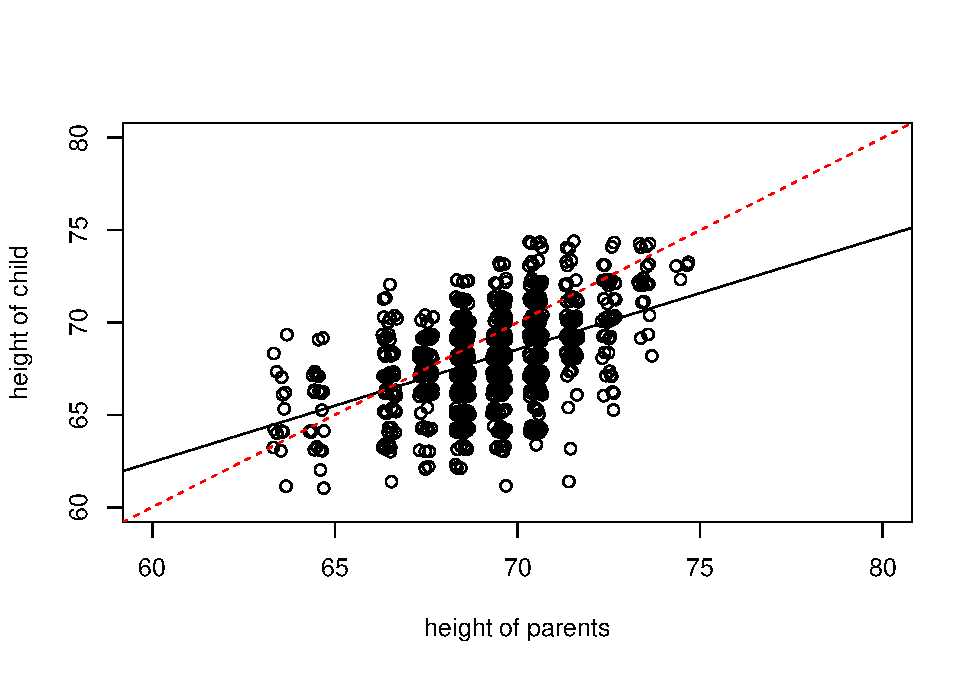
\includegraphics{RegressModelDataCamp_files/figure-latex/unnamed-chunk-3-1.pdf}

\begin{Shaded}
\begin{Highlighting}[]
\KeywordTok{summary}\NormalTok{(}\KeywordTok{lm}\NormalTok{(heights}\OperatorTok{$}\NormalTok{child_ht}\OperatorTok{~}\NormalTok{heights}\OperatorTok{$}\NormalTok{parent_ht))}
\end{Highlighting}
\end{Shaded}

\begin{verbatim}

Call:
lm(formula = heights$child_ht ~ heights$parent_ht)

Residuals:
    Min      1Q  Median      3Q     Max 
-8.2577 -1.4280  0.1323  1.5720  5.7918 

Coefficients:
                  Estimate Std. Error t value Pr(>|t|)    
(Intercept)       25.84856    2.69009   9.609   <2e-16 ***
heights$parent_ht  0.60992    0.03882  15.710   <2e-16 ***
---
Signif. codes:  0 '***' 0.001 '**' 0.01 '*' 0.05 '.' 0.1 ' ' 1

Residual standard error: 2.26 on 926 degrees of freedom
Multiple R-squared:  0.2104,    Adjusted R-squared:  0.2096 
F-statistic: 246.8 on 1 and 926 DF,  p-value: < 2.2e-16
\end{verbatim}

\chapter{Regression and the Normal
Distribution}\label{regression-and-the-normal-distribution}

\textbf{Chapter description}

Regression analysis is a statistical method that is widely used in many
fields of study, with actuarial science being no exception. This chapter
introduces the role of the normal distribution in regression and the use
of logarithmic transformations in specifying regression relationships.

\section{Fitting a normal
distribution}\label{fitting-a-normal-distribution}

\begin{center}\rule{0.5\linewidth}{\linethickness}\end{center}

In this section, you learn how to:

\begin{itemize}
\tightlist
\item
  Calculate and interpret two basic summary statistics
\item
  Fit a data set to a normal curve
\item
  Calculate probabilities under a standard normal curve
\end{itemize}

\begin{center}\rule{0.5\linewidth}{\linethickness}\end{center}

\subsection{Video}\label{video}

\subsubsection*{Video Overhead Details}\label{video-overhead-details}
\addcontentsline{toc}{subsubsection}{Video Overhead Details}

Show Overhead A Details. Description of the data

\hypertarget{toggleOver1.1A}{}
To illustrate a data set that can be analyzed using regression methods,
we consider some data included in Galton's 1885 paper. These data
include the heights of 928 adult children (child\_ht), together with an
index of their parents' height (parent\_ht). Here, all female heights
were multiplied by 1.08, and the index was created by taking the average
of the father's height and rescaled mother's height. Galton was aware
that the parents' and the adult child's height could each be adequately
approximated by a normal curve. In developing regression analysis, he
provided a single model for the joint distribution of heights.

\begin{Shaded}
\begin{Highlighting}[]
\NormalTok{heights <-}\StringTok{ }\KeywordTok{read.csv}\NormalTok{(}\StringTok{"CSVData}\CharTok{\textbackslash{}\textbackslash{}}\StringTok{galton_height.csv"}\NormalTok{, }\DataTypeTok{header =} \OtherTok{TRUE}\NormalTok{)}
\CommentTok{#heights <- read.csv("https://assets.datacamp.com/production/repositories/2610/datasets/c85ede6c205d22049e766bd08956b225c576255b/galton_height.csv", header = TRUE)}
\KeywordTok{plot}\NormalTok{(}\KeywordTok{jitter}\NormalTok{(heights}\OperatorTok{$}\NormalTok{parent_ht),}\KeywordTok{jitter}\NormalTok{(heights}\OperatorTok{$}\NormalTok{child_ht), }\DataTypeTok{ylim =} \KeywordTok{c}\NormalTok{(}\DecValTok{60}\NormalTok{,}\DecValTok{80}\NormalTok{), }\DataTypeTok{xlim =} \KeywordTok{c}\NormalTok{(}\DecValTok{60}\NormalTok{,}\DecValTok{80}\NormalTok{),}
     \DataTypeTok{ylab =} \StringTok{"height of child"}\NormalTok{, }\DataTypeTok{xlab =} \StringTok{"height of parents"}\NormalTok{)}
\KeywordTok{abline}\NormalTok{(}\KeywordTok{lm}\NormalTok{(heights}\OperatorTok{$}\NormalTok{child_ht}\OperatorTok{~}\NormalTok{heights}\OperatorTok{$}\NormalTok{parent_ht))}
\KeywordTok{abline}\NormalTok{(}\DecValTok{0}\NormalTok{,}\DecValTok{1}\NormalTok{,}\DataTypeTok{col =} \StringTok{"red"}\NormalTok{)}
\end{Highlighting}
\end{Shaded}

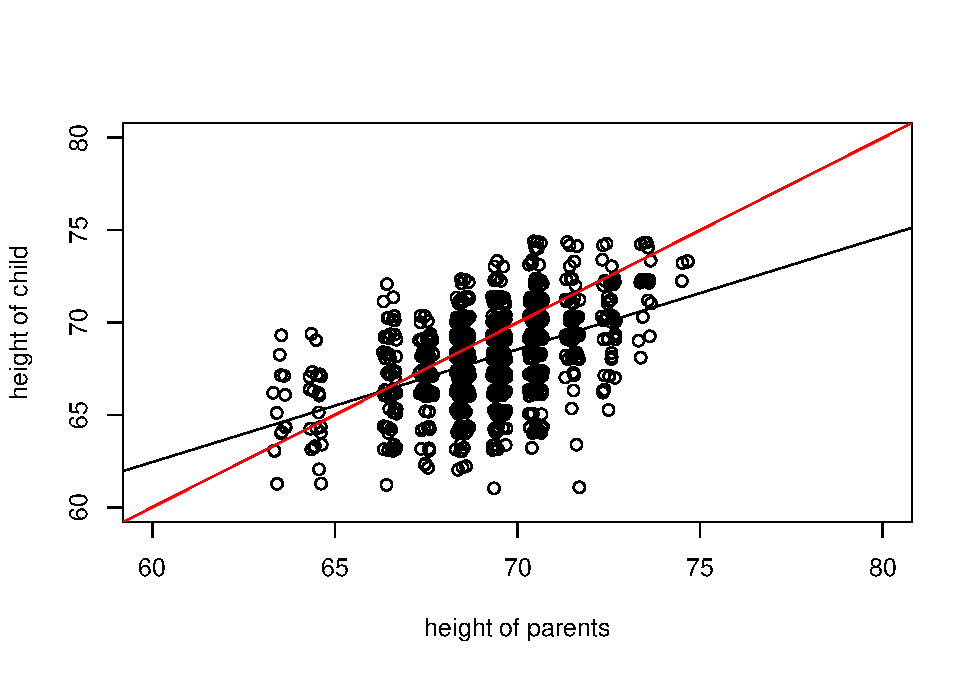
\includegraphics{RegressModelDataCamp_files/figure-latex/unnamed-chunk-4-1.pdf}

Show Overhead B Details. Read and examine data structure

\hypertarget{toggleOver1.1B}{}
The data has already been read into a dataset called \texttt{heights}.
Examine the \emph{structure} of the data with the function
\href{https://www.rdocumentation.org/packages/utils/versions/3.5.0/topics/str/}{str()}
and use the
\href{https://www.rdocumentation.org/packages/utils/versions/3.5.0/topics/head/}{head()}
command to looks at the first few records.

\begin{Shaded}
\begin{Highlighting}[]
\NormalTok{heights <-}\StringTok{ }\KeywordTok{read.csv}\NormalTok{(}\StringTok{"CSVData}\CharTok{\textbackslash{}\textbackslash{}}\StringTok{galton_height.csv"}\NormalTok{,}\DataTypeTok{header =} \OtherTok{TRUE}\NormalTok{)}
\CommentTok{#heights <- read.csv("https://assets.datacamp.com/production/repositories/2610/datasets/c85ede6c205d22049e766bd08956b225c576255b/galton_height.csv", header = TRUE)}
\KeywordTok{str}\NormalTok{(heights)}
\KeywordTok{head}\NormalTok{(heights)}
\end{Highlighting}
\end{Shaded}

\begin{verbatim}
'data.frame':   928 obs. of  2 variables:
 $ child_ht : num  72.2 73.2 73.2 73.2 68.2 ...
 $ parent_ht: num  74.5 74.5 74.5 74.5 73.5 73.5 73.5 73.5 73.5 73.5 ...
  child_ht parent_ht
1     72.2      74.5
2     73.2      74.5
3     73.2      74.5
4     73.2      74.5
5     68.2      73.5
6     69.2      73.5
\end{verbatim}

Show Overhead C Details. Summary stats for parents' height

\hypertarget{toggleOver1.1C}{}
Next, examine the distribution of the child's height and then examine
the distribution of the parents height.

\begin{Shaded}
\begin{Highlighting}[]
\NormalTok{ht_par <-}\StringTok{ }\NormalTok{heights}\OperatorTok{$}\NormalTok{parent_ht}
\KeywordTok{hist}\NormalTok{(ht_par)}
\end{Highlighting}
\end{Shaded}

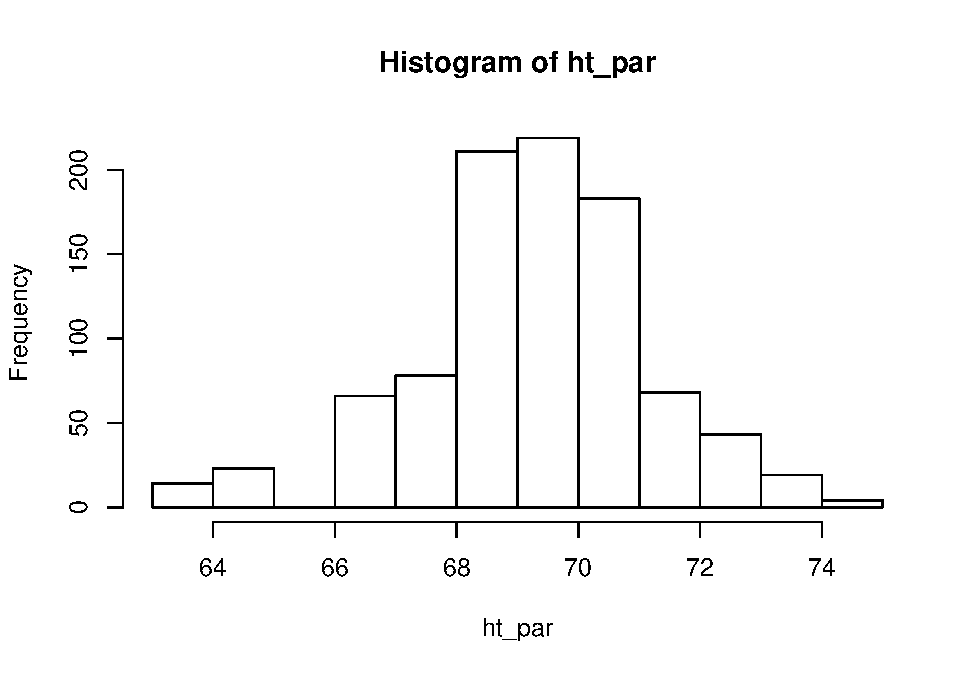
\includegraphics{RegressModelDataCamp_files/figure-latex/unnamed-chunk-6-1.pdf}

\begin{Shaded}
\begin{Highlighting}[]
\KeywordTok{mean}\NormalTok{(ht_par)}
\KeywordTok{sd}\NormalTok{(ht_par)}
\end{Highlighting}
\end{Shaded}

\begin{verbatim}
[1] 69.26293
[1] 1.912274
\end{verbatim}

Show Overhead D. Fit a normal curve to parents' height details

\hypertarget{toggleOver1.1D}{}
\begin{Shaded}
\begin{Highlighting}[]
\NormalTok{(mparent <-}\StringTok{ }\KeywordTok{mean}\NormalTok{(ht_par))}
\NormalTok{(sdparent <-}\StringTok{ }\KeywordTok{sd}\NormalTok{(ht_par))}
\NormalTok{x <-}\StringTok{ }\KeywordTok{seq}\NormalTok{(}\DecValTok{60}\NormalTok{, }\DecValTok{80}\NormalTok{,}\DataTypeTok{by =} \FloatTok{0.1}\NormalTok{)}
\KeywordTok{hist}\NormalTok{(ht_par, }\DataTypeTok{freq =} \OtherTok{FALSE}\NormalTok{)}
\KeywordTok{lines}\NormalTok{(x, }\KeywordTok{dnorm}\NormalTok{(x, }\DataTypeTok{mean =}\NormalTok{ mparent, }\DataTypeTok{sd =}\NormalTok{ sdparent), }\DataTypeTok{col =} \StringTok{"blue"}\NormalTok{)}
\end{Highlighting}
\end{Shaded}

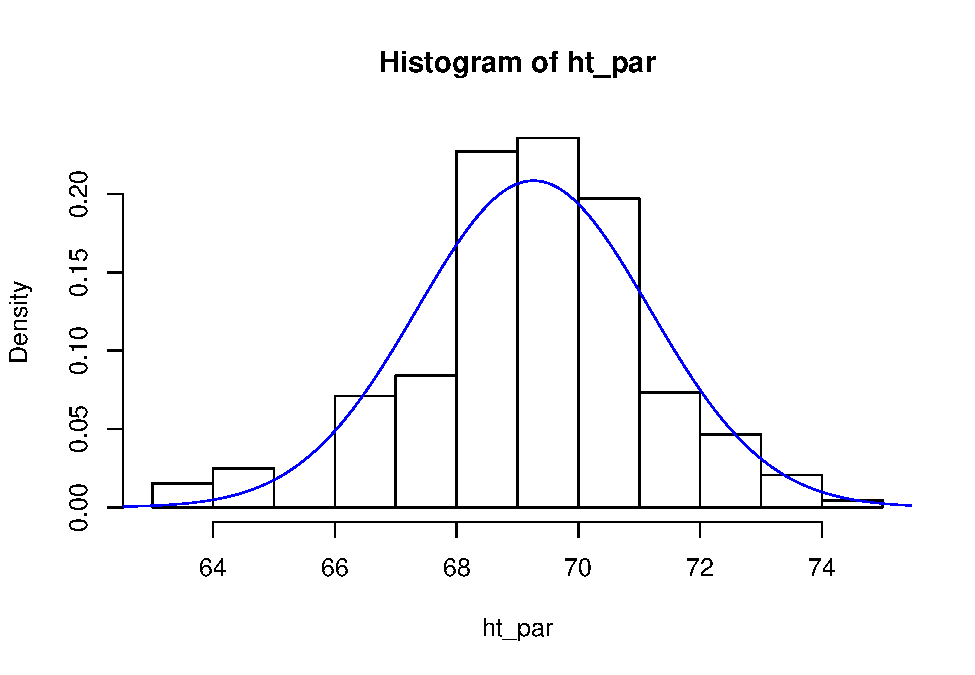
\includegraphics{RegressModelDataCamp_files/figure-latex/unnamed-chunk-7-1.pdf}

\begin{verbatim}
[1] 69.26293
[1] 1.912274
\end{verbatim}

Show Overhead E Details. Use the normal approximation to determine the
probability of the height of tall parents

\hypertarget{toggleOver1.1E}{}
\begin{Shaded}
\begin{Highlighting}[]
\NormalTok{TallHeight <-}\StringTok{ }\DecValTok{72}
\KeywordTok{pnorm}\NormalTok{(TallHeight, }\DataTypeTok{mean =}\NormalTok{ mparent, }\DataTypeTok{sd =}\NormalTok{ sdparent)}
\KeywordTok{pnorm}\NormalTok{(}\DecValTok{72}\NormalTok{, }\DataTypeTok{mean =} \KeywordTok{mean}\NormalTok{(ht_par), }\DataTypeTok{sd =} \KeywordTok{sd}\NormalTok{(ht_par))}
\NormalTok{(StdUnitsTallHeight <-}\StringTok{ }\NormalTok{(TallHeight }\OperatorTok{-}\StringTok{ }\NormalTok{mparent)}\OperatorTok{/}\NormalTok{sdparent)}
\KeywordTok{pnorm}\NormalTok{(StdUnitsTallHeight, }\DataTypeTok{mean =} \DecValTok{0}\NormalTok{, }\DataTypeTok{sd =} \DecValTok{1}\NormalTok{)}
\end{Highlighting}
\end{Shaded}

\begin{verbatim}
[1] 0.9238302
[1] 0.9238302
[1] 1.431317
[1] 0.9238302
\end{verbatim}

\subsection{Exercise. Fitting Galton's height
data}\label{exercise.-fitting-galtons-height-data}

\textbf{Assignment Text}

The Galton data has already been read into a dataframe called
\texttt{heights}. These data include the heights of 928 adult children
\texttt{child\_ht}, together with an index of their parents' height
\texttt{parent\_ht}. The video explored the distribution of the parents'
height; in this assignment, we investigate the distribution of the
heights of the adult children.

\textbf{Instructions}

\begin{itemize}
\tightlist
\item
  Define the height of an adult child as a global variable
\item
  Use the function
  \href{https://www.rdocumentation.org/packages/base/versions/3.5.0/topics/mean/}{mean()}
  to calculate the mean and the function
  \href{https://www.rdocumentation.org/packages/base/versions/3.5.0/topics/sd/}{sd()}
  to calculate the standard deviation
\item
  Use the normal approximation and the function
  \href{https://www.rdocumentation.org/packages/stats/versions/3.5.0/topics/Normal/}{pnorm()}
  determine the probability that an adult child's height is less than 72
  inches
\end{itemize}

\textbf{Hint.} Remember that we can reference a variable, say
\texttt{var}, from a data set such as \texttt{heights}, as
\texttt{heights\$var}.

eyJsYW5ndWFnZSI6InIiLCJwcmVfZXhlcmNpc2VfY29kZSI6IiNoZWlnaHRzIDwtIHJlYWQuY3N2KFwiQ1NWRGF0YVxcXFxnYWx0b25faGVpZ2h0LmNzdlwiLGhlYWRlciA9IFRSVUUpXG5oZWlnaHRzIDwtIHJlYWQuY3N2KFwiaHR0cHM6Ly9hc3NldHMuZGF0YWNhbXAuY29tL3Byb2R1Y3Rpb24vcmVwb3NpdG9yaWVzLzI2MTAvZGF0YXNldHMvYzg1ZWRlNmMyMDVkMjIwNDllNzY2YmQwODk1NmIyMjVjNTc2MjU1Yi9nYWx0b25faGVpZ2h0LmNzdlwiLCBoZWFkZXIgPSBUUlVFKSIsInNhbXBsZSI6IiNEZWZpbmUgdGhlIGdsb2JhbCB2YXJpYWJsZVxuaHRfY2hpbGQgPC0gX19fXG5cbiNDYWxjdWxhdGUgdGhlIG1lYW4gaGVpZ2h0XG5tY2hpbGQgPC0gX19fXG5tY2hpbGRcblxuI0NhbGN1bGF0ZSB0aGUgc3RhbmRhcmQgZGV2aWF0aW9uIG9mIGhlaWdodHNcbnNkY2hpbGQgPC0gX19fXG5zZGNoaWxkXG5cbiNEZXRlcm1pbmUgdGhlIHByb2JhYmlsaXR5IHRoYXQgdGhlIGhlaWdodCBpcyBsZXNzIHRoYW4gNzJcbl9fXyg3MiwgbWVhbj1tY2hpbGQsIHNkPXNkY2hpbGQpIiwic29sdXRpb24iOiIjIFNvbHV0aW9uXG5odF9jaGlsZCA8LSBoZWlnaHRzJGNoaWxkX2h0XG5tY2hpbGQgPC0gbWVhbihodF9jaGlsZClcbnNkY2hpbGQgPC0gc2QoaHRfY2hpbGQpXG5tY2hpbGRcbnNkY2hpbGRcbnBub3JtKDcyLCBtZWFuID0gbWNoaWxkLCBzZCA9IHNkY2hpbGQpIiwic2N0IjoiZXgoKSAlPiUgY2hlY2tfb2JqZWN0KFwiaHRfY2hpbGRcIix1bmRlZmluZWRfbXNnPVwiTWFrZSBzdXJlIHlvdSBhc3NpZ24gdGhlIGNoaWxkcmVuJ3MgaGlnaHQgdG8gaHRfY2hpbGRcIikgJT4lIGNoZWNrX2VxdWFsKGluY29ycmVjdF9tc2c9XCJSZW1lbWJlciB0aGF0IGluIG9yZGVyIHRvIGNhbGwgYSBzcGVjaWZpYyBjb2x1bW4gZnJvbSBhIGRhdGFmcmFtZSwgdXNlIHRoZSAkIG9wZXJhdG9yXCIpXG5leCgpICU+JSBjaGVja19vYmplY3QoXCJtY2hpbGRcIikgICU+JSBjaGVja19lcXVhbCgpXG5leCgpICU+JSBjaGVja19vYmplY3QoXCJzZGNoaWxkXCIpICU+JSBjaGVja19lcXVhbCgpXG5leCgpICU+JSBjaGVja19vYmplY3QoXCJwclwiKSAlPiUgY2hlY2tfZXF1YWwoKVxuc3VjY2Vzc19tc2coXCJFeGNlbGxlbnQhIFdpdGggdGhpcyBwcm9jZWR1cmUsIHlvdSBjYW4gbm93IGNhbGN1bGF0ZSBwcm9iYWJpbGl0aWVzIGZvciBhbnkgZGlzdHJpYnV0aW9uIHVzaW5nIGEgbm9ybWFsIGN1cnZlIGFwcHJveGltYXRpb24uXCIpIn0=

\subsection{Exercise. Visualizing child's height
distribution}\label{exercise.-visualizing-childs-height-distribution}

\textbf{Assignment Text}

As in the prior exercise, from the Galton dataset \texttt{heights}, the
heights of 928 adult children have been used to create a global variable
called \texttt{ht\_child}. We also have basic summary statistics, the
mean height \texttt{mchild} and the standard deviation of heights in
\texttt{sdchild}. In this exercise, we explore the fit of the normal
curve to this distribution.

\textbf{Instructions}

\begin{itemize}
\tightlist
\item
  To visualize the distribution, use the function
  \href{https://www.rdocumentation.org/packages/graphics/versions/3.5.0/topics/hist/}{hist()}
  to calculate the histogram. Use the \texttt{freq\ =\ FALSE} option to
  give a histogram with proportions instead of counts.
\item
  Use the function
  \href{https://www.rdocumentation.org/packages/base/versions/3.5.0/topics/seq}{seq()}
  to determine a sequence that can be used for plotting. Then, with the
  function
  \href{https://www.rdocumentation.org/packages/graphics/versions/3.5.0/topics/lines/}{lines()},
  superimpose a normal curve on the histogram
\item
  Determine the probability that a child's height is greater than 72
  inches
\end{itemize}

\textbf{Hint 1.} Use the function
\href{https://www.rdocumentation.org/packages/stats/versions/3.5.0/topics/Normal/}{dnorm()}
to calculate the normal density, similar to the cumulative probabilites
that you calculated using
\href{https://www.rdocumentation.org/packages/stats/versions/3.5.0/topics/Normal/}{pnorm()}

\textbf{Hint 2.} To calculate probabilities greater that an amount,
simply use 1 minus the cumulative probability

\textbf{Pre-exercise code}

eyJsYW5ndWFnZSI6InIiLCJwcmVfZXhlcmNpc2VfY29kZSI6IiNoZWlnaHRzIDwtIHJlYWQuY3N2KFwiQ1NWRGF0YVxcXFxnYWx0b25faGVpZ2h0LmNzdlwiLGhlYWRlciA9IFRSVUUpXG5oZWlnaHRzIDwtIHJlYWQuY3N2KFwiaHR0cHM6Ly9hc3NldHMuZGF0YWNhbXAuY29tL3Byb2R1Y3Rpb24vcmVwb3NpdG9yaWVzLzI2MTAvZGF0YXNldHMvYzg1ZWRlNmMyMDVkMjIwNDllNzY2YmQwODk1NmIyMjVjNTc2MjU1Yi9nYWx0b25faGVpZ2h0LmNzdlwiLCBoZWFkZXIgPSBUUlVFKVxuaHRfY2hpbGQgPC0gaGVpZ2h0cyRjaGlsZF9odFxubWNoaWxkIDwtIG1lYW4oaHRfY2hpbGQpXG5zZGNoaWxkIDwtIHNkKGh0X2NoaWxkKSIsInNhbXBsZSI6IiNWaXN1YWxpemUgdGhlIERpc3RyaWJ1dGlvblxuX19fKF9fXywgZnJlcSA9IEZBTFNFKVxuXG4jRGV0ZXJtaW5lIGEgc2VxdWVuY2UuIFRoZW4sIGdyYXBoIGEgaGlzdG9ncmFtIHdpdGggYSBub3JtYWwgY3VydmUgc3VwZXJpbXBvc2VkXG54IDwtIHNlcSg2MCwgODAsYnkgPSAwLjEpXG5fX18oeCwgZG5vcm0oeCxtZWFuID0gbWNoaWxkLCBzZCA9IHNkY2hpbGQpLCBjb2wgPSBcImJsdWVcIilcblxuIyBEZXRlcm1pbmUgdGhlIHByb2JhYmlsaXR5IHRoYXQgYSBjaGlsZCdzIGhlaWdodCBpcyBncmVhdGVyIHRoYW4gNzJcbnByb2IgPC0gMSAtIFxucHJvYiIsInNvbHV0aW9uIjoiaGlzdChodF9jaGlsZCwgZnJlcSA9IEZBTFNFKVxueCA8LSBzZXEoNjAsIDgwLGJ5ID0gMC4xKVxubGluZXMoeCwgZG5vcm0oeCwgbWVhbiA9IG1jaGlsZCwgc2QgPSBzZGNoaWxkKSwgY29sID0gXCJibHVlXCIpXG5wcm9iIDwtIDEgLSBwbm9ybSg3MiwgbWVhbiA9IG1jaGlsZCAsIHNkID0gc2RjaGlsZClcbnByb2IiLCJzY3QiOiJzdWNjZXNzX21zZyhcIkV4Y2VsbGVudCEgVmlzdWFsaXppbmcgYSBkaXN0cmlidXRpb24sIGVzcGVjaWFsbHkgd2l0aCByZWZlcmVuY2UgdG8gYSBub3JtYWwsIGlzIGltcG9ydGFudCBmb3IgY29tbXVuaWNhdGluZyByZXN1bHRzIG9mIHlvdXIgYW5hbHlzaXMuXCIpIn0=

\section{Visualizing distributions}\label{visualizing-distributions}

\begin{center}\rule{0.5\linewidth}{\linethickness}\end{center}

In this section, you learn how to:

\begin{itemize}
\tightlist
\item
  Calculate and interpret distributions using histograms
\item
  Calculate and interpret distributions using density plots
\end{itemize}

\begin{center}\rule{0.5\linewidth}{\linethickness}\end{center}

\subsection{Video}\label{video-1}

\subsubsection*{Video Overhead Details}\label{video-overhead-details-1}
\addcontentsline{toc}{subsubsection}{Video Overhead Details}

Show Overhead Details. Data description

\hypertarget{toggleOver1.2}{}
\begin{center}\rule{0.5\linewidth}{\linethickness}\end{center}

For our first look at an insurance data set, we consider data from
Rempala and Derrig (2005). They considered claims arising from
automobile bodily injury insurance coverages. These are amounts incurred
for outpatient medical treatments that arise from automobile accidents,
typically sprains, broken collarbones and the like. The data consists of
a sample of 272 claims from Massachusetts that were closed in 2001 (by
``closed,'' we mean that the claim is settled and no additional
liabilities can arise from the same accident). Rempala and Derrig were
interested in developing procedures for handling mixtures of ``typical''
claims and others from providers who reported claims fraudulently. For
this sample, we consider only those typical claims, ignoring the
potentially fraudulent ones.

\begin{Shaded}
\begin{Highlighting}[]
\CommentTok{# Reformat Data Set}
\NormalTok{injury <-}\StringTok{ }\KeywordTok{read.csv}\NormalTok{(}\StringTok{"CSVData}\CharTok{\textbackslash{}\textbackslash{}}\StringTok{MassBodilyInjury.csv"}\NormalTok{,}\DataTypeTok{header =} \OtherTok{TRUE}\NormalTok{)}
\KeywordTok{str}\NormalTok{(injury)}
\KeywordTok{head}\NormalTok{(injury)}
\CommentTok{#  PICK THE SUBSET OF THE DATA CORRESPONDING TO PROVIDER A}
\NormalTok{injury2 <-}\StringTok{ }\KeywordTok{subset}\NormalTok{(injury, providerA }\OperatorTok{!}\StringTok{ }\ErrorTok{=}\StringTok{ }\DecValTok{0}\NormalTok{ )}
\NormalTok{injury2}\OperatorTok{$}\NormalTok{claims <-}\StringTok{ }\DecValTok{1000}\OperatorTok{*}\NormalTok{injury2}\OperatorTok{$}\NormalTok{claims}
\NormalTok{injury2}\OperatorTok{$}\NormalTok{logclaims <-}\StringTok{ }\KeywordTok{log}\NormalTok{(injury2}\OperatorTok{$}\NormalTok{claims)}
\NormalTok{injury3 <-}\StringTok{ }\NormalTok{injury2[}\KeywordTok{c}\NormalTok{(}\StringTok{"claims"}\NormalTok{,}\StringTok{"logclaims"}\NormalTok{)]}
\CommentTok{#write.csv(injury3,"CSVData\textbackslash{}\textbackslash{}MassBI.csv",row.names = FALSE)}
\end{Highlighting}
\end{Shaded}

Show Overhead A Details. Bring in Data, Introduce Logarithmic Claims

\hypertarget{toggleOver1.2A}{}
\begin{Shaded}
\begin{Highlighting}[]
\NormalTok{injury <-}\StringTok{ }\KeywordTok{read.csv}\NormalTok{(}\StringTok{"CSVData}\CharTok{\textbackslash{}\textbackslash{}}\StringTok{MassBI.csv"}\NormalTok{,}\DataTypeTok{header =} \OtherTok{TRUE}\NormalTok{)}
\CommentTok{#  CHECK THE NAMES, DIMENSION IN THE FILE AND LIST THE FIRST 8 OBSERVATIONS  ;}
\KeywordTok{str}\NormalTok{(injury)}
\KeywordTok{head}\NormalTok{(injury)}
\KeywordTok{attach}\NormalTok{(injury)}
\NormalTok{claims <-}\StringTok{ }\NormalTok{injury}\OperatorTok{$}\NormalTok{claims}
\KeywordTok{par}\NormalTok{(}\DataTypeTok{mfrow =} \KeywordTok{c}\NormalTok{(}\DecValTok{1}\NormalTok{, }\DecValTok{2}\NormalTok{))}
\KeywordTok{hist}\NormalTok{(claims)}
\KeywordTok{hist}\NormalTok{(logclaims)}
\end{Highlighting}
\end{Shaded}

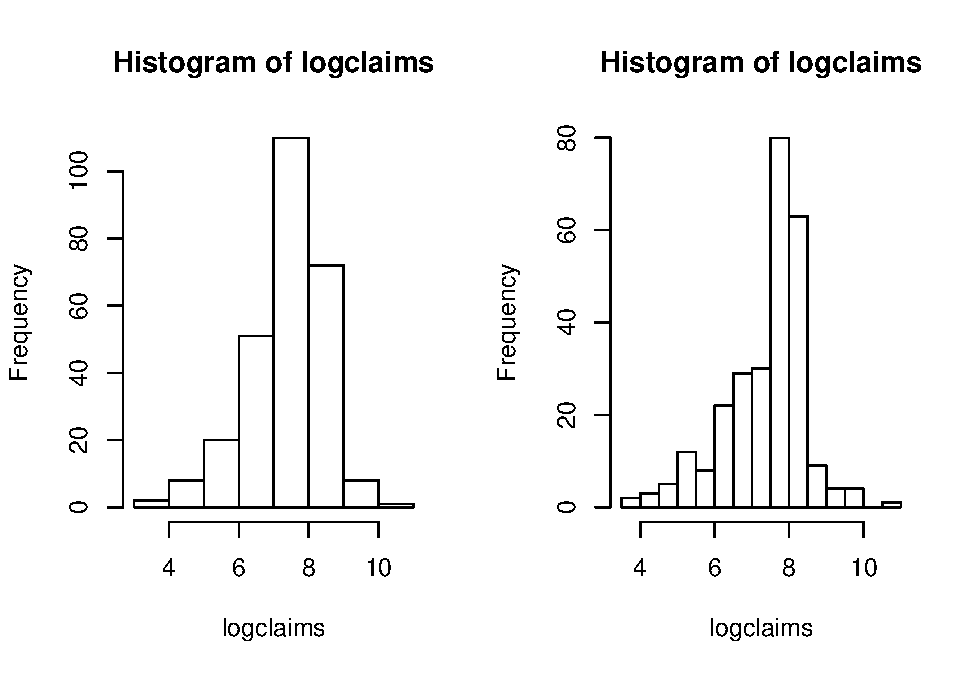
\includegraphics{RegressModelDataCamp_files/figure-latex/unnamed-chunk-19-1.pdf}

\begin{verbatim}
'data.frame':   272 obs. of  2 variables:
 $ claims   : int  45 47 70 75 77 92 117 117 140 145 ...
 $ logclaims: num  3.81 3.85 4.25 4.32 4.34 ...
  claims logclaims
1     45  3.806662
2     47  3.850148
3     70  4.248495
4     75  4.317488
5     77  4.343805
6     92  4.521789
\end{verbatim}

Show Overhead B Details. Show how to get a finer grid for histograms

\hypertarget{toggleOver1.2B}{}
\begin{Shaded}
\begin{Highlighting}[]
\KeywordTok{par}\NormalTok{(}\DataTypeTok{mfrow =} \KeywordTok{c}\NormalTok{(}\DecValTok{1}\NormalTok{, }\DecValTok{2}\NormalTok{))}
\KeywordTok{hist}\NormalTok{(logclaims)}
\KeywordTok{hist}\NormalTok{(logclaims,}\DataTypeTok{breaks =} \DecValTok{15}\NormalTok{)}
\end{Highlighting}
\end{Shaded}

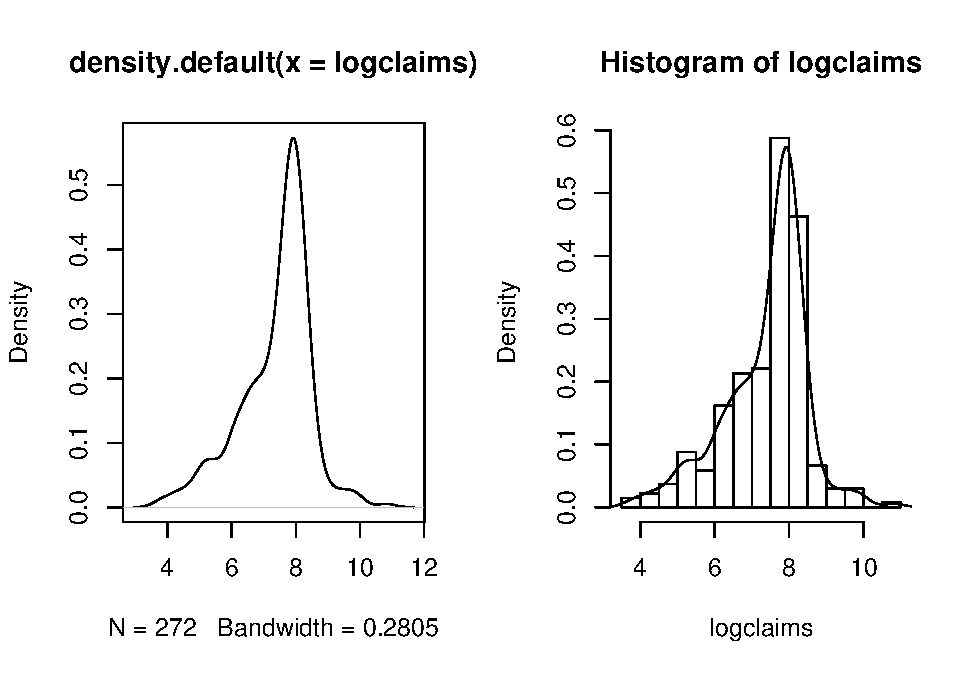
\includegraphics{RegressModelDataCamp_files/figure-latex/unnamed-chunk-20-1.pdf}

Show Overhead C Details. Introduce the density plot

\hypertarget{toggleOver1.2C}{}
\begin{Shaded}
\begin{Highlighting}[]
\KeywordTok{par}\NormalTok{(}\DataTypeTok{mfrow =} \KeywordTok{c}\NormalTok{(}\DecValTok{1}\NormalTok{, }\DecValTok{2}\NormalTok{))}
\KeywordTok{plot}\NormalTok{(}\KeywordTok{density}\NormalTok{(logclaims))}
\KeywordTok{hist}\NormalTok{(logclaims, }\DataTypeTok{breaks =} \DecValTok{15}\NormalTok{,}\DataTypeTok{freq =} \OtherTok{FALSE}\NormalTok{)}
\KeywordTok{lines}\NormalTok{(}\KeywordTok{density}\NormalTok{(logclaims))}
\end{Highlighting}
\end{Shaded}

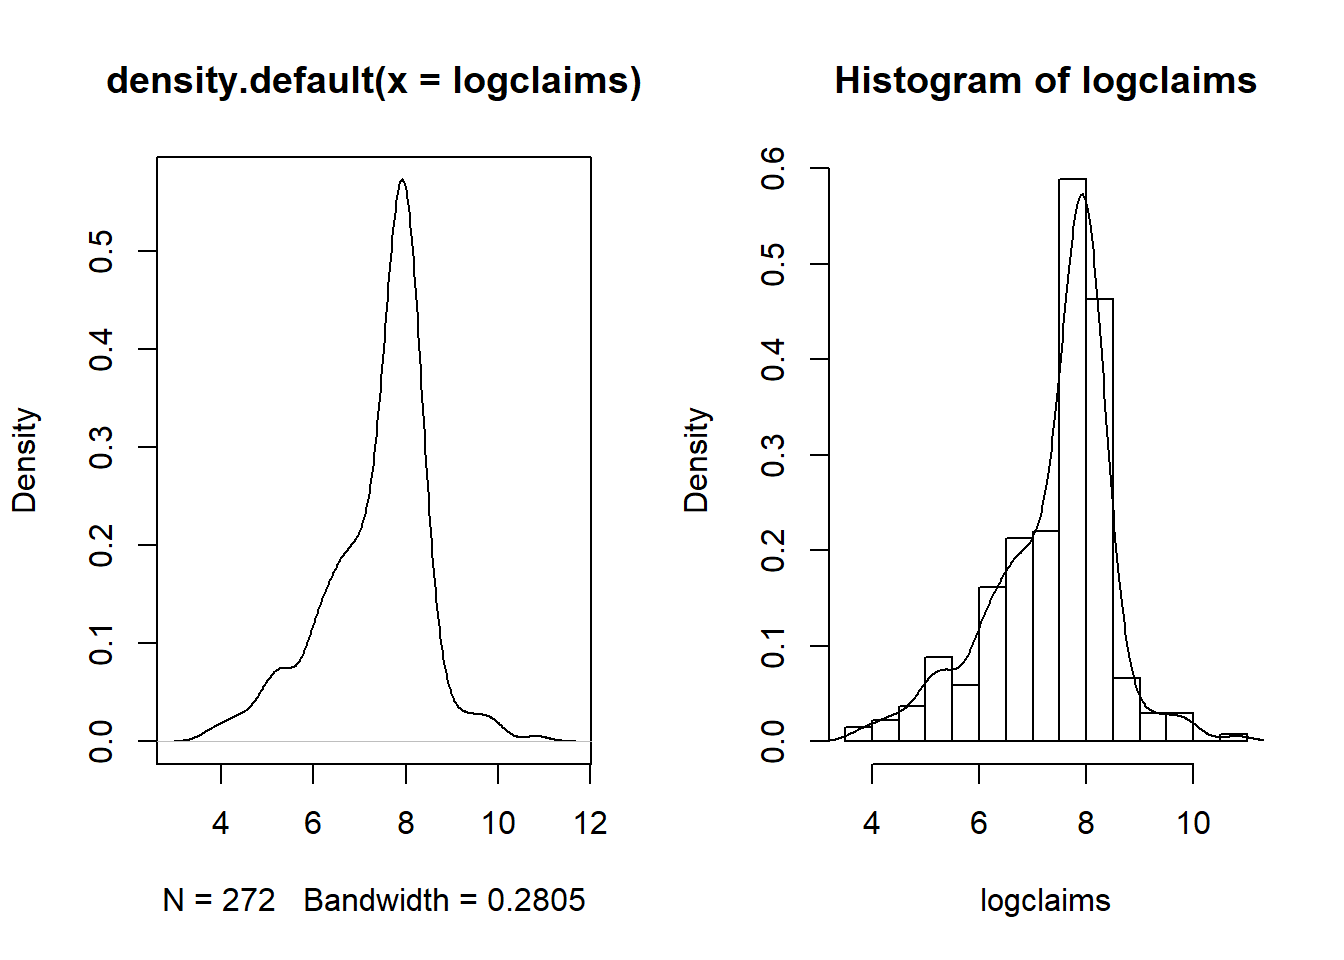
\includegraphics{RegressModelDataCamp_files/figure-latex/unnamed-chunk-21-1.pdf}

\subsection{Exercise. Visualizing bodily injury claims with density
plots}\label{exercise.-visualizing-bodily-injury-claims-with-density-plots}

\textbf{Assignment Text}

In the prior video, you learned about the Massachusetts bodily injury
dataset. This dataframe, \texttt{injury}, has been read in and the
global variable \texttt{claims} has been created. This assignment
reviews the
\href{https://www.rdocumentation.org/packages/graphics/versions/3.5.0/topics/hist/}{hist()}
function for visualizing distributions and allows you to explore density
plotting, a smoothed version of the histogram.

\textbf{Instructions}

\begin{itemize}
\tightlist
\item
  Use the function
  \href{https://www.rdocumentation.org/packages/base/versions/3.5.0/topics/log/}{log()}
  to create the logarithmic version of the claims variable
\item
  Calculate a histogram of logarithmic with 40 bins using an option in
  the
  \href{https://www.rdocumentation.org/packages/graphics/versions/3.5.0/topics/hist/}{hist()}
  function, \texttt{breaks\ =}.
\item
  Create a density plot of logarithmic claims using the functions
  \href{https://www.rdocumentation.org/packages/graphics/versions/3.5.0/topics/plot/}{plot()}
  and
  \href{https://www.rdocumentation.org/packages/stats/versions/3.5.0/topics/density/}{density()}.
\item
  Repeat the density plot, this time using a more refined bandwidth
  equal to 0.03. Use an option in the
  \href{https://www.rdocumentation.org/packages/stats/versions/3.5.0/topics/density/}{density()}
  function, \texttt{bw\ =}.
\end{itemize}

eyJsYW5ndWFnZSI6InIiLCJwcmVfZXhlcmNpc2VfY29kZSI6IiNpbmp1cnkgPC0gcmVhZC5jc3YoXCJDU1ZEYXRhXFxcXE1hc3NCSS5jc3ZcIixoZWFkZXIgPSBUUlVFKVxuaW5qdXJ5IDwtIHJlYWQuY3N2KFwiaHR0cHM6Ly9hc3NldHMuZGF0YWNhbXAuY29tL3Byb2R1Y3Rpb24vcmVwb3NpdG9yaWVzLzI2MTAvZGF0YXNldHMvOGNjYTE5ZDA1MDNmY2Y2ZTlkMzBkOWNiOTEyZGU1YmE5NWVjYjljMS9NYXNzQkkuY3N2XCIsIGhlYWRlciA9IFRSVUUpXG5jbGFpbXMgPC0gaW5qdXJ5JGNsYWltcyIsInNhbXBsZSI6IiNDcmVhdGUgdGhlIGxvZ2FyaXRobWljIGNsYWltcyB2YXJpYWJsZVxubG9nY2xhaW1zIDwtIF9fX1xuXG4jQ3JlYXRlIGEgaGlzdG9ncmFtIHVzaW5zIDQwIGJpbnNcbl9fXyhsb2djbGFpbXMsIGJyZWFrcyA9IDQwLGZyZXEgPSBGQUxTRSlcbmJveCgpXG5cbiMgQ3JlYXRlIGEgZGVuc2l0eSBwbG90IG9mIGxvZ2FyaXRobWljIGNsYWltc1xucGxvdChfX18obG9nY2xhaW1zKSlcblxuIyBDcmVhdGUgYSBkZW5zaXR5IHBsb3Qgb2YgbG9nYXJpdGhtaWMgY2xhaW1zIHdpdGggYSBzbWFsbGVyIGJhbmR3aWR0aFxuX19fIiwic29sdXRpb24iOiJsb2djbGFpbXMgPC0gbG9nKGNsYWltcylcbmhpc3QobG9nY2xhaW1zICwgYnJlYWtzID0gNDAsZnJlcSA9IEZBTFNFKVxuYm94KClcbnBsb3QoZGVuc2l0eShsb2djbGFpbXMpKVxucGxvdChkZW5zaXR5KGxvZ2NsYWltcywgYncgPSAwLjAzKSkiLCJzY3QiOiJzdWNjZXNzX21zZyhcIkV4Y2VsbGVudCEgVmlzdWFsaXppbmcgdGhlIGRpc3RyaWJ1dGlvbiBpcyBpbXBvcnRhbnQgYW5kIHNtb290aGluZyB0ZWNobmlxdWVzIGFsbG93IHZpZXdlcnMgdG8gc2VlIGltcG9ydGFudCBwYXR0ZXJucyB3aXRob3V0IGJlaW5nIGRpc3RyYWN0ZWQgYnkgcmFuZG9tIGZsdWN0YXRpb25zLlwiKSJ9

\section{Summarizing distributions}\label{summarizing-distributions}

\begin{center}\rule{0.5\linewidth}{\linethickness}\end{center}

In this section, you learn how to:

\begin{itemize}
\tightlist
\item
  Calculate and interpret basic summary statistics
\item
  Calculate and interpret distributions using boxplots
\item
  Calculate and interpret distributions using qq plots
\end{itemize}

\begin{center}\rule{0.5\linewidth}{\linethickness}\end{center}

\subsection{Video}\label{video-2}

\subsubsection*{Video Overhead Details}\label{video-overhead-details-2}
\addcontentsline{toc}{subsubsection}{Video Overhead Details}

Show Overhead A Details. Summary statistics

\hypertarget{toggleOver1.3A}{}
\begin{Shaded}
\begin{Highlighting}[]
\NormalTok{injury <-}\StringTok{ }\KeywordTok{read.csv}\NormalTok{(}\StringTok{"CSVData}\CharTok{\textbackslash{}\textbackslash{}}\StringTok{MassBI.csv"}\NormalTok{,}\DataTypeTok{header =} \OtherTok{TRUE}\NormalTok{)}
\CommentTok{#injury <- read.csv("https://assets.datacamp.com/production/repositories/2610/datasets/8cca19d0503fcf6e9d30d9cb912de5ba95ecb9c1/MassBI.csv", header = TRUE)}
\KeywordTok{attach}\NormalTok{(injury)}

\CommentTok{# SUMMARY STATISTICS}
\KeywordTok{summary}\NormalTok{(injury)}
\KeywordTok{sd}\NormalTok{(claims);}\KeywordTok{sd}\NormalTok{(logclaims)}
\KeywordTok{length}\NormalTok{(claims)}
\end{Highlighting}
\end{Shaded}

\begin{verbatim}
     claims          logclaims     
 Min.   :   45.0   Min.   : 3.807  
 1st Qu.:  892.5   1st Qu.: 6.794  
 Median : 2210.0   Median : 7.701  
 Mean   : 2697.7   Mean   : 7.388  
 3rd Qu.: 3215.0   3rd Qu.: 8.076  
 Max.   :50000.0   Max.   :10.820  
[1] 3944.445
[1] 1.10093
[1] 272
\end{verbatim}

Show Overhead B Details. Boxplot

\hypertarget{toggleOver1.3B}{}
\begin{Shaded}
\begin{Highlighting}[]
\CommentTok{# BASIC BOXPLOT}
\KeywordTok{boxplot}\NormalTok{(logclaims)}
\end{Highlighting}
\end{Shaded}

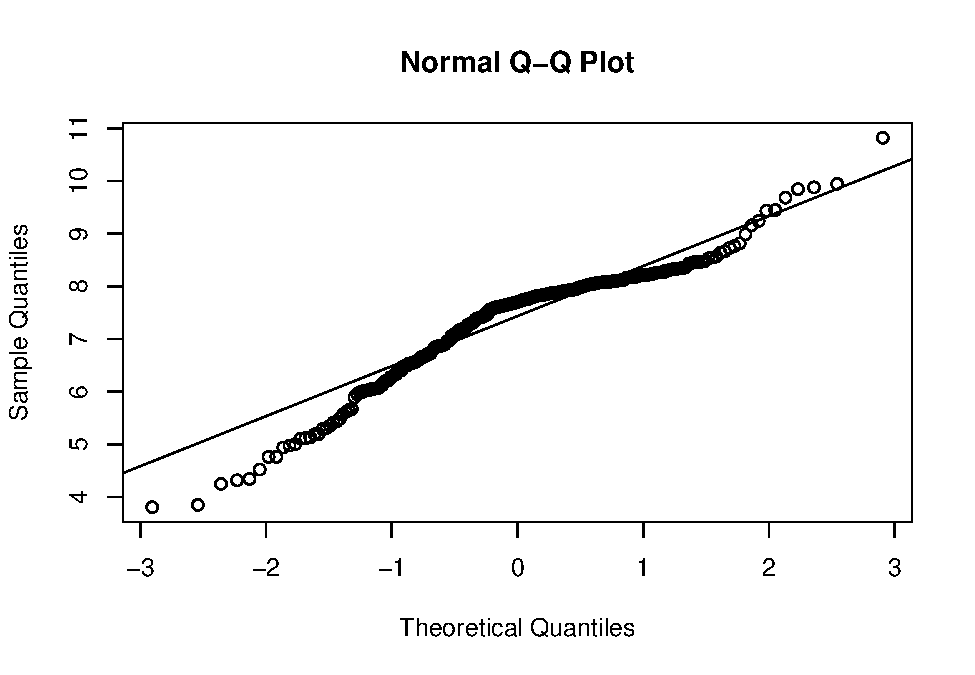
\includegraphics{RegressModelDataCamp_files/figure-latex/unnamed-chunk-27-1.pdf}

\begin{Shaded}
\begin{Highlighting}[]
\KeywordTok{quantile}\NormalTok{(logclaims, }\DataTypeTok{probs =} \FloatTok{0.75}\NormalTok{)}

\CommentTok{# BOXPLOT WITH ANNOTATION}
\KeywordTok{boxplot}\NormalTok{(logclaims, }\DataTypeTok{main =} \StringTok{"Boxplot of logclaims"}\NormalTok{)}
\KeywordTok{text}\NormalTok{(}\DecValTok{1}\NormalTok{,  }\FloatTok{7.6}\NormalTok{,  }\StringTok{"median"}\NormalTok{, }\DataTypeTok{cex =} \FloatTok{0.7}\NormalTok{)}
\KeywordTok{text}\NormalTok{(}\DecValTok{1}\NormalTok{,  }\FloatTok{6.55}\NormalTok{, }\StringTok{"25th percentile"}\NormalTok{, }\DataTypeTok{cex =} \FloatTok{0.7}\NormalTok{)}
\KeywordTok{text}\NormalTok{(}\DecValTok{1}\NormalTok{,  }\FloatTok{7.95}\NormalTok{, }\StringTok{"75th percentile"}\NormalTok{, }\DataTypeTok{cex =} \FloatTok{0.7}\NormalTok{)}
\KeywordTok{arrows}\NormalTok{(}\FloatTok{1.05}\NormalTok{, }\FloatTok{4.9}\NormalTok{, }\FloatTok{1.05}\NormalTok{, }\FloatTok{3.6}\NormalTok{, }\DataTypeTok{col =} \StringTok{"blue"}\NormalTok{, }\DataTypeTok{code =} \DecValTok{3}\NormalTok{, }\DataTypeTok{angle =} \DecValTok{20}\NormalTok{, }\DataTypeTok{length =} \FloatTok{0.1}\NormalTok{)}
\KeywordTok{text}\NormalTok{(}\FloatTok{1.1}\NormalTok{,  }\FloatTok{4.4}\NormalTok{, }\StringTok{"outliers"}\NormalTok{, }\DataTypeTok{cex =} \FloatTok{0.7}\NormalTok{)}
\KeywordTok{text}\NormalTok{(}\FloatTok{1.1}\NormalTok{, }\FloatTok{10.9}\NormalTok{, }\StringTok{"outlier"}\NormalTok{,  }\DataTypeTok{cex =} \FloatTok{0.7}\NormalTok{)}
\end{Highlighting}
\end{Shaded}

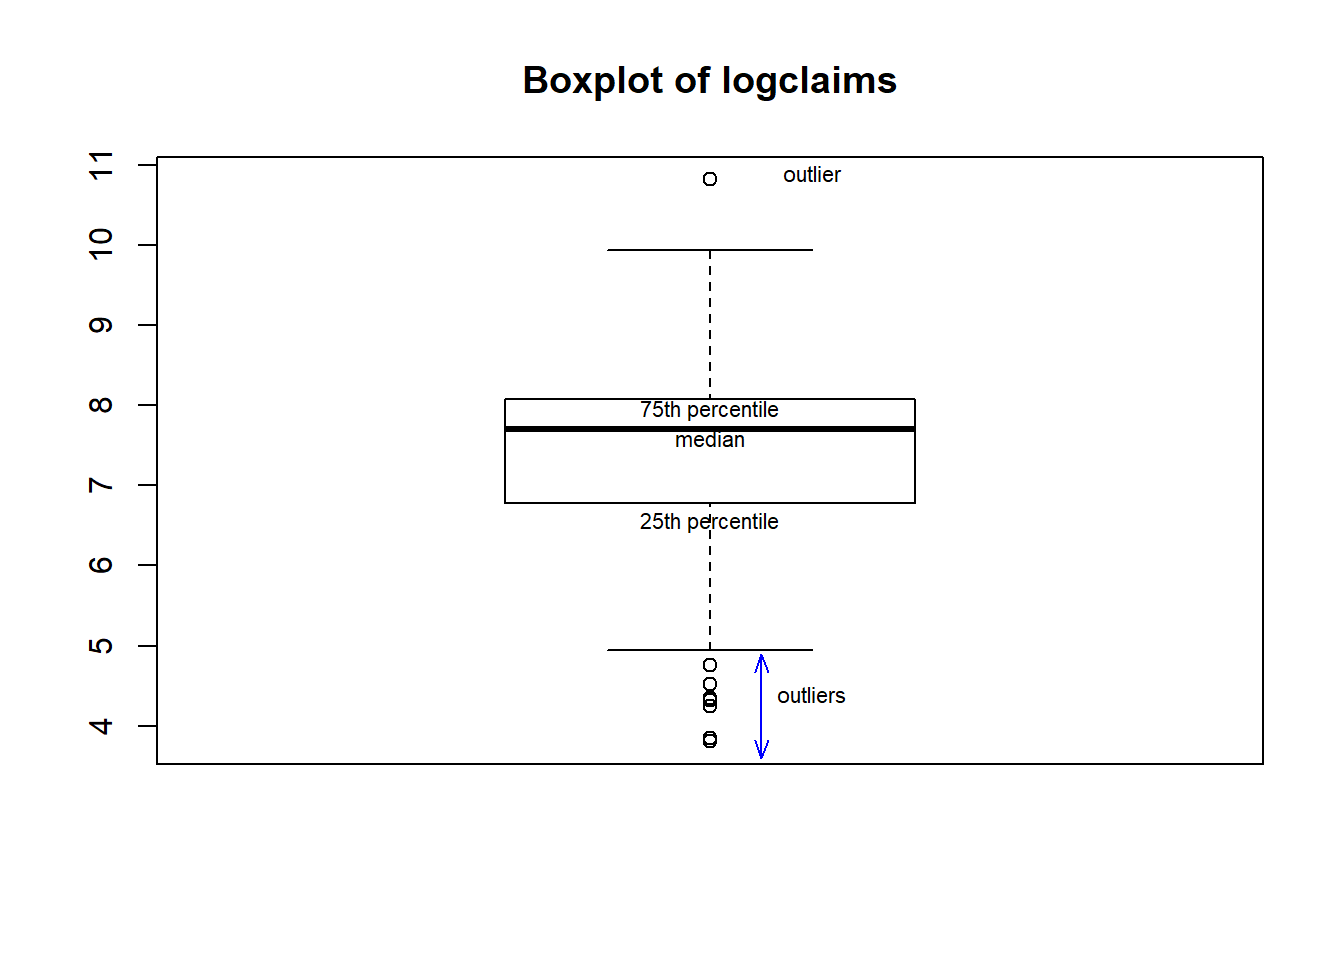
\includegraphics{RegressModelDataCamp_files/figure-latex/unnamed-chunk-27-2.pdf}

\begin{verbatim}
     75% 
8.075579 
\end{verbatim}

Show Overhead C Details. QQ Plot

\hypertarget{toggleOver1.3C}{}
\begin{Shaded}
\begin{Highlighting}[]
\KeywordTok{summary}\NormalTok{(injury)}
\KeywordTok{quantile}\NormalTok{(claims, }\DataTypeTok{probs =} \FloatTok{0.75}\NormalTok{)}
\KeywordTok{quantile}\NormalTok{(logclaims, }\DataTypeTok{probs =} \FloatTok{0.75}\NormalTok{)}
\KeywordTok{log}\NormalTok{(}\KeywordTok{quantile}\NormalTok{(claims, }\DataTypeTok{probs =} \FloatTok{0.75}\NormalTok{))}
\KeywordTok{qnorm}\NormalTok{(}\DataTypeTok{p =} \FloatTok{0.75}\NormalTok{, }\DataTypeTok{mean =} \KeywordTok{mean}\NormalTok{(logclaims), }\DataTypeTok{sd =} \KeywordTok{sd}\NormalTok{(logclaims))}
\NormalTok{(}\KeywordTok{qnorm}\NormalTok{(}\DataTypeTok{p =} \FloatTok{0.75}\NormalTok{, }\DataTypeTok{mean =} \KeywordTok{mean}\NormalTok{(logclaims), }\DataTypeTok{sd =} \KeywordTok{sd}\NormalTok{(logclaims)) }\OperatorTok{-}\KeywordTok{mean}\NormalTok{(logclaims)) }\OperatorTok{/}
\StringTok{       }\KeywordTok{sd}\NormalTok{(logclaims)}
\KeywordTok{qnorm}\NormalTok{(}\DataTypeTok{p =} \FloatTok{0.75}\NormalTok{, }\DataTypeTok{mean =} \DecValTok{0}\NormalTok{, }\DataTypeTok{sd =} \DecValTok{1}\NormalTok{)}

\CommentTok{#  QUANTILE - QUANTILE PLOT}
\KeywordTok{qqnorm}\NormalTok{(logclaims)}
\KeywordTok{qqline}\NormalTok{(logclaims)   }
\end{Highlighting}
\end{Shaded}

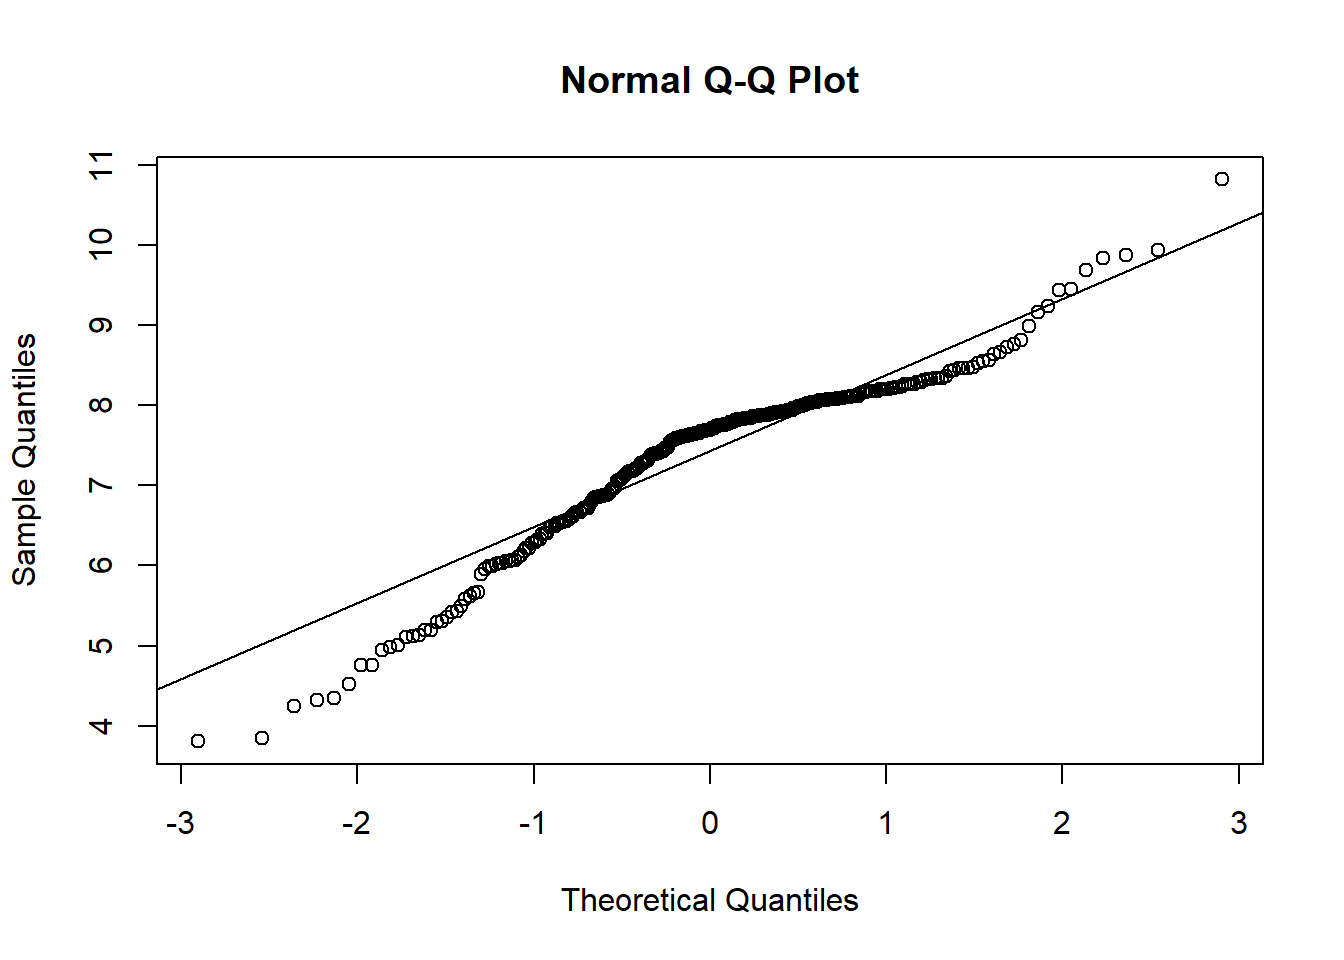
\includegraphics{RegressModelDataCamp_files/figure-latex/unnamed-chunk-28-1.pdf}

\begin{verbatim}
     claims          logclaims     
 Min.   :   45.0   Min.   : 3.807  
 1st Qu.:  892.5   1st Qu.: 6.794  
 Median : 2210.0   Median : 7.701  
 Mean   : 2697.7   Mean   : 7.388  
 3rd Qu.: 3215.0   3rd Qu.: 8.076  
 Max.   :50000.0   Max.   :10.820  
 75% 
3215 
     75% 
8.075579 
     75% 
8.075583 
[1] 8.131056
[1] 0.6744898
[1] 0.6744898
\end{verbatim}

\subsection{Exercise. Summarizing bodily injury claims with box and qq
plots}\label{exercise.-summarizing-bodily-injury-claims-with-box-and-qq-plots}

\textbf{Assignment Text}

The Massachusetts bodily injury data has already been read and used to
create the global variable \texttt{claims} representing bodily injury
claims. The previous video showed how to present the distribution of
logarithmic claims which appeared to be approximately normally
distributed. However, users are not really interested in log dollars but
want to know about a unit of measurement that is more intuitive, such as
dollars.

So this assignment is based on claims, not the logarithmic version. You
will use the functions
\href{https://www.rdocumentation.org/packages/graphics/versions/3.5.0/topics/boxplot/}{boxplot()}
and
\href{https://www.rdocumentation.org/packages/stats/versions/3.5.0/topics/qqnorm/}{qqnorm()}
to visualize the distribution through boxplots and quantile-quantile, or
qq-, plots. But, because we are working with such a skewed distribution,
do not be surprised that it is difficult to interpret these results
readily.

\textbf{Instructions}

\begin{itemize}
\tightlist
\item
  Produce a box plot for claims
\item
  Determine the 25th empirical percentile for claims using the
  \href{https://www.rdocumentation.org/packages/stats/versions/3.5.0/topics/quantile/}{quantile()}
  function.
\item
  Determine the 25th percentile for claims based on a normal
  distribution using the
  \href{https://www.rdocumentation.org/packages/stats/versions/3.5.0/topics/Normal/}{qnorm()}
  function.
\item
  Produce a normal qq plot for claims using the function
  \href{https://www.rdocumentation.org/packages/stats/versions/3.5.0/topics/qqnorm/}{qqnorm()}.
  The
  \href{https://www.rdocumentation.org/packages/stats/versions/3.5.0/topics/qqnorm/}{qqline()}
  function is handy for producing a reference line.
\end{itemize}

\textbf{Hint.} Note that
\href{https://www.rdocumentation.org/packages/stats/versions/3.5.0/topics/Normal/}{qnorm()}
(one \texttt{q}) is for a normal quantile and
\href{https://www.rdocumentation.org/packages/stats/versions/3.5.0/topics/qqnorm/}{qqnorm()}.
(two \texttt{q}'s!) is for the normal qq plot

eyJsYW5ndWFnZSI6InIiLCJwcmVfZXhlcmNpc2VfY29kZSI6IiNpbmp1cnkgPC0gcmVhZC5jc3YoXCJDU1ZEYXRhXFxcXE1hc3NCSS5jc3ZcIiwgaGVhZGVyID0gVFJVRSlcbmluanVyeSA8LSByZWFkLmNzdihcImh0dHBzOi8vYXNzZXRzLmRhdGFjYW1wLmNvbS9wcm9kdWN0aW9uL3JlcG9zaXRvcmllcy8yNjEwL2RhdGFzZXRzLzhjY2ExOWQwNTAzZmNmNmU5ZDMwZDljYjkxMmRlNWJhOTVlY2I5YzEvTWFzc0JJLmNzdlwiLCBoZWFkZXIgPSBUUlVFKVxuY2xhaW1zIDwtIGluanVyeSRjbGFpbXMiLCJzYW1wbGUiOiIjUHJvZHVjZSBhIGJveCBwbG90IGZvciBjbGFpbXNcbl9fXyhjbGFpbXMpXG5cbiNEZXRlcm1pbmUgdGhlIDI1dGggZW1waXJpY2FsIHBlcmNlbnRpbGUgZm9yIGNsYWltc1xucTI1IDwtIF9fXyhjbGFpbXMsIHByb2JzID0gX19fKVxucTI1XG5cbiNEZXRlcm1pbmUgdGhlIDI1dGggcGVyY2VudGlsZSBmb3IgY2xhaW1zIGJhc2VkIG9uIGEgbm9ybWFsIGRpc3RyaWJ1dGlvblxucW4yNSA8LSBfX18ocCA9IF9fXywgbWVhbiA9IG1lYW4oY2xhaW1zKSwgc2QgPSBzZChjbGFpbXMpKVxucW4yNVxuXG4jUHJvZHVjZSBhIG5vcm1hbCBxcSBwbG90IGZvciBjbGFpbXNcbl9fXyhjbGFpbXMpXG5fX18oY2xhaW1zKSIsInNvbHV0aW9uIjoiIyBTb2x1dGlvblxuYm94cGxvdChjbGFpbXMpXG5xMjUgPC0gcXVhbnRpbGUoY2xhaW1zLCBwcm9icyA9IDAuMjUpXG5xMjVcbnFuMjUgPC0gcW5vcm0ocCA9IDAuMjUsIG1lYW4gPSBtZWFuKGNsYWltcyksIHNkID0gc2QoY2xhaW1zKSlcbnFuMjVcbnFxbm9ybShjbGFpbXMpXG5xcWxpbmUoY2xhaW1zKSAgICIsInNjdCI6InN1Y2Nlc3NfbXNnKFwiQ29uZ3JhdHVsYXRpb25zIG9uIGxlYXJuaW5nIGFib3V0IGJveCBhbmQgcXEgcGxvdHMuIEFsdGhvdWdoIHlvdSBhcmUgdW5saWtlbHkgdG8gc2hvdyB0aGVzZSBwbG90cyB0byBjb25zdW1lcnMgb2YgeW91ciBhbmFseXNpcywgeW91IHdpbGwgZmluZCB0aGVtIHVzZWZ1bCB0b29scyBmb3IgZXhwbG9yaW5nIG11bHRpdmFyaWF0ZSBhc3BlY3RzIG9mIGRhdGEuXCIpIn0=

\subsection{Exercise. Effects on distributions of removing the largest
claim}\label{exercise.-effects-on-distributions-of-removing-the-largest-claim}

\textbf{Assignment Text}

The Massachusetts bodily injury dataframe \texttt{injury} has been read
in; our focus is on the \texttt{claims} variable in that dataset.

In the previous exercise, we learned that the Massachusetts bodily
injury \texttt{claims} distribution was not even close to approximately
normal (as evidenced by the box and qq- plots). Non-normality may be
induced by skewness (that we will handle via transformations in the next
section). But, seeming non-normality can also be induced by one or two
very large observations (called an \emph{outlier} later in the course).
So, this exercise examines the effects on the distribution of removing
the largest claims.

\textbf{Instructions}

\begin{itemize}
\tightlist
\item
  Use the function
  \href{https://www.rdocumentation.org/packages/utils/versions/3.5.0/topics/head}{tail()}
  to examine the \texttt{injury} dataset and identify the largest claim
\item
  Use the function
  \href{https://www.rdocumentation.org/packages/base/versions/3.5.0/topics/subset}{subset()}
  to create a subset omitting the largest claim
\item
  Compare the summary statistics of the omitted claim distribution to
  the full distribution
\item
  Compare the two distributions visually via histograms plotted next to
  another. \texttt{par(mfrow\ =\ c(1,\ 2))} is used to organize the
  plots you create. Do not alter this code.
\end{itemize}

\textbf{Hint.} For this data set, the {[}subset(){]} argument
\texttt{claims\ \textless{}\ 25000} will keep all but the largest claim

eyJsYW5ndWFnZSI6InIiLCJwcmVfZXhlcmNpc2VfY29kZSI6IiNpbmp1cnkgPC0gcmVhZC5jc3YoXCJDU1ZEYXRhXFxcXE1hc3NCSS5jc3ZcIiwgaGVhZGVyID0gVFJVRSlcbmluanVyeSA8LSByZWFkLmNzdihcImh0dHBzOi8vYXNzZXRzLmRhdGFjYW1wLmNvbS9wcm9kdWN0aW9uL3JlcG9zaXRvcmllcy8yNjEwL2RhdGFzZXRzLzhjY2ExOWQwNTAzZmNmNmU5ZDMwZDljYjkxMmRlNWJhOTVlY2I5YzEvTWFzc0JJLmNzdlwiLCBoZWFkZXIgPSBUUlVFKVxuY2xhaW1zIDwtIGluanVyeSRjbGFpbXMiLCJzYW1wbGUiOiIjIEV4YW1pbmUgdGhlIHRhaWwgb2YgdGhlIGBpbmp1cnlgIGRhdGFzZXRcbnRhaWwoX19fKVxuXG4jIENyZWF0ZSBhIHN1YnNldCBvbWl0dGluZyB0aGUgbGFyZ2VzdCBjbGFpbVxuaW5qdXJ5MiA8LSBzdWJzZXQoaW5qdXJ5LCBfX18pXG5cbiMgQ29tcGFyZSB0aGUgc3VtbWFyeSBzdGF0aXN0aWNzIG9mIHRoZSBvbWl0dGVkIGNsYWltIGRpc3RyaWJ1dGlvbiB0byB0aGUgZnVsbCBkaXN0cmlidXRpb25cbnN1bW1hcnkoX19fKVxuc3VtbWFyeShpbmp1cnkyKVxuXG4jIENvbXBhcmUgdGhlIHR3byBkaXN0cmlidXRpb25zIHZpc3VhbGx5IHZpYSBoaXN0b2dyYW1zIHBsb3R0ZWQgbmV4dCB0byBhbm90aGVyXG5wYXIobWZyb3cgPSBjKDEsIDIpKVxuaGlzdChfX18sIGZyZXEgPSBGQUxTRSwgIG1haW4gPSBcIkZ1bGwgRGF0YVwiKVxuaGlzdChfX18sIGZyZXEgPSBGQUxTRSwgIG1haW4gPSBcIkxhcmdlc3QgQ2xhaW0gT21pdHRlZFwiKSIsInNvbHV0aW9uIjoidGFpbChpbmp1cnkpXG5pbmp1cnkyIDwtIHN1YnNldChpbmp1cnksIGNsYWltcyA8IDI1MDAwIClcbnN1bW1hcnkoaW5qdXJ5KVxuc3VtbWFyeShpbmp1cnkyKVxuXG5wYXIobWZyb3cgPSBjKDEsIDIpKVxuaGlzdChjbGFpbXMsIGZyZXEgPSBGQUxTRSwgIG1haW4gPSBcIkZ1bGwgRGF0YVwiKVxuaGlzdChpbmp1cnkyJGNsYWltcywgZnJlcSA9IEZBTFNFLCAgbWFpbiA9IFwiTGFyZ2VzdCBDbGFpbSBPbWl0dGVkXCIpIiwic2N0Ijoic3VjY2Vzc19tc2coXCJDb25ncmF0dWxhdGlvbnMhIFRoZSBnb2FsIG9mIHByZWRpY3RpdmUgbW9kZWxpbmcgaXMgdG8gZGlzY292ZXIgcGF0dGVybnMgaW4gdGhlIGRhdGEuIEhvd2V2ZXIsIHNvbWV0aW1lcyBzZWVtaW5nICdwYXR0ZXJucycgYXJlIHRoZSByZXN1bHQgb2Ygb25lIG9yIHR3byB1bnVzdWFsIG9ic2VydmF0aW9ucy4gVW51c3VhbCBvYnNlcnZhdGlvbnMgbWF5IGJlIGR1ZSB0byBpbmNvcnJlY3QgZGF0YSBnYXRoZXJpbmcgcHJvY2VkdXJlcyBvciBqdXN0IGR1ZSB0byB3aWxkIGZsdWN0dWF0aW9ucyBpbiBhIHByb2Nlc3Mgb2YgaW50ZXJlc3QgYnV0IGFyZSBjb21tb24gaW4gcHJlZGljdGl2ZSBtb2RlbGluZy5cIikifQ==

\section{Transformations}\label{transformations}

\begin{center}\rule{0.5\linewidth}{\linethickness}\end{center}

In this exercise, you learn how to:

\begin{itemize}
\tightlist
\item
  Symmetrize a skewed distribution using a logarithmic transformation
\end{itemize}

\begin{center}\rule{0.5\linewidth}{\linethickness}\end{center}

\subsection{Video}\label{video-3}

\subsubsection*{Video Overhead Details}\label{video-overhead-details-3}
\addcontentsline{toc}{subsubsection}{Video Overhead Details}

Show Overhead A Details. Simulate a moderately skewed distribution, with
transforms

\hypertarget{toggleOver1.4A}{}
\begin{Shaded}
\begin{Highlighting}[]
\CommentTok{#  FIGURE 1.7 - SIMULATE CHI-SQUARE, CREATE 3 TRANSFORMATIONS}
\KeywordTok{set.seed}\NormalTok{(}\DecValTok{1237}\NormalTok{)                  }\CommentTok{# set the seed of the random number generator}
                                \CommentTok{# allows us to replicate results}
\NormalTok{X1 <-}\StringTok{ }\DecValTok{10000}\OperatorTok{*}\KeywordTok{rchisq}\NormalTok{(}\DecValTok{500}\NormalTok{, }\DataTypeTok{df =} \DecValTok{2}\NormalTok{) }\CommentTok{# generate variables randomly from a skewed distribution}
\NormalTok{X2 <-}\StringTok{ }\NormalTok{X1}\OperatorTok{^}\NormalTok{(}\FloatTok{0.5}\NormalTok{)                  }\CommentTok{# square root transform, could also use sqrt(X1)}
\NormalTok{X3 <-}\StringTok{ }\KeywordTok{log}\NormalTok{(X1)                   }\CommentTok{# logarithmic transform}
\NormalTok{X4 <-}\StringTok{ }\OperatorTok{-}\DecValTok{1}\OperatorTok{/}\NormalTok{X1                     }\CommentTok{# negative reciprocal transform}
\end{Highlighting}
\end{Shaded}

Show Overhead B Details. Visualize the distributions

\hypertarget{toggleOver1.4B}{}
\begin{Shaded}
\begin{Highlighting}[]
\KeywordTok{par}\NormalTok{(}\DataTypeTok{mfrow =} \KeywordTok{c}\NormalTok{(}\DecValTok{2}\NormalTok{, }\DecValTok{2}\NormalTok{), }\DataTypeTok{cex =}\NormalTok{ .}\DecValTok{75}\NormalTok{, }\DataTypeTok{mar =} \KeywordTok{c}\NormalTok{(}\DecValTok{3}\NormalTok{,}\DecValTok{5}\NormalTok{,}\FloatTok{1.5}\NormalTok{,}\DecValTok{0}\NormalTok{))}
\KeywordTok{hist}\NormalTok{(X1, }\DataTypeTok{freq =} \OtherTok{FALSE}\NormalTok{,  }\DataTypeTok{nclass =} \DecValTok{16}\NormalTok{, }\DataTypeTok{main =} \StringTok{""}\NormalTok{, }\DataTypeTok{xlab =} \StringTok{""}\NormalTok{, }\DataTypeTok{ylab =} \StringTok{""}\NormalTok{, }
      \DataTypeTok{las =} \DecValTok{1}\NormalTok{, }\DataTypeTok{yaxt =} \StringTok{"n"}\NormalTok{,}\DataTypeTok{xlim =} \KeywordTok{c}\NormalTok{(}\DecValTok{0}\NormalTok{,}\DecValTok{200000}\NormalTok{),}\DataTypeTok{ylim =} \KeywordTok{c}\NormalTok{(}\DecValTok{0}\NormalTok{,.}\DecValTok{00005}\NormalTok{))}
\KeywordTok{axis}\NormalTok{(}\DecValTok{2}\NormalTok{, }\DataTypeTok{at =} \KeywordTok{seq}\NormalTok{(}\DecValTok{0}\NormalTok{,.}\DecValTok{00005}\NormalTok{,.}\DecValTok{00001}\NormalTok{),}\DataTypeTok{las =} \DecValTok{1}\NormalTok{, }\DataTypeTok{cex =}\NormalTok{ .}\DecValTok{3}\NormalTok{, }
  \DataTypeTok{labels =} \KeywordTok{c}\NormalTok{(}\StringTok{"0"}\NormalTok{, }\StringTok{"0.00001"}\NormalTok{, }\StringTok{"0.00002"}\NormalTok{,}\StringTok{"0.00003"}\NormalTok{, }\StringTok{"0.00004"}\NormalTok{, }\StringTok{"0.00005"}\NormalTok{))}
\KeywordTok{mtext}\NormalTok{(}\StringTok{"Density"}\NormalTok{, }\DataTypeTok{side =} \DecValTok{2}\NormalTok{, }\DataTypeTok{at =}\NormalTok{ .}\DecValTok{000055}\NormalTok{, }\DataTypeTok{las =} \DecValTok{1}\NormalTok{, }\DataTypeTok{cex =}\NormalTok{ .}\DecValTok{75}\NormalTok{)}
\KeywordTok{mtext}\NormalTok{(}\StringTok{"y"}\NormalTok{, }\DataTypeTok{side =} \DecValTok{1}\NormalTok{, }\DataTypeTok{cex =}\NormalTok{ .}\DecValTok{75}\NormalTok{, }\DataTypeTok{line =} \DecValTok{2}\NormalTok{)}

\KeywordTok{par}\NormalTok{(}\DataTypeTok{mar =} \KeywordTok{c}\NormalTok{(}\DecValTok{3}\NormalTok{,}\DecValTok{4}\NormalTok{,}\FloatTok{1.5}\NormalTok{,}\FloatTok{0.2}\NormalTok{))}
\KeywordTok{hist}\NormalTok{(X2, }\DataTypeTok{freq =} \OtherTok{FALSE}\NormalTok{,  }\DataTypeTok{nclass =} \DecValTok{16}\NormalTok{, }\DataTypeTok{main =} \StringTok{""}\NormalTok{, }\DataTypeTok{xlab =} \StringTok{""}\NormalTok{, }\DataTypeTok{ylab =} \StringTok{""}\NormalTok{, }
      \DataTypeTok{las =} \DecValTok{1}\NormalTok{,}\DataTypeTok{xlim =} \KeywordTok{c}\NormalTok{(}\DecValTok{0}\NormalTok{,}\DecValTok{400}\NormalTok{), }\DataTypeTok{ylim =} \KeywordTok{c}\NormalTok{(}\DecValTok{0}\NormalTok{,.}\DecValTok{008}\NormalTok{))}
\KeywordTok{mtext}\NormalTok{(}\StringTok{"Density"}\NormalTok{, }\DataTypeTok{side =} \DecValTok{2}\NormalTok{, }\DataTypeTok{at =}\NormalTok{ .}\DecValTok{0088}\NormalTok{, }\DataTypeTok{las =} \DecValTok{1}\NormalTok{, }\DataTypeTok{cex =}\NormalTok{ .}\DecValTok{75}\NormalTok{)}
\KeywordTok{mtext}\NormalTok{(}\StringTok{"Square root of y"}\NormalTok{, }\DataTypeTok{side =} \DecValTok{1}\NormalTok{, }\DataTypeTok{cex =}\NormalTok{ .}\DecValTok{75}\NormalTok{, }\DataTypeTok{line =} \DecValTok{2}\NormalTok{)}

\KeywordTok{par}\NormalTok{(}\DataTypeTok{mar =} \KeywordTok{c}\NormalTok{(}\FloatTok{3.2}\NormalTok{,}\DecValTok{5}\NormalTok{,}\DecValTok{1}\NormalTok{,}\DecValTok{0}\NormalTok{))}
\KeywordTok{hist}\NormalTok{(X3,  }\DataTypeTok{freq =} \OtherTok{FALSE}\NormalTok{,  }\DataTypeTok{nclass =} \DecValTok{16}\NormalTok{, }\DataTypeTok{main =} \StringTok{""}\NormalTok{, }\DataTypeTok{xlab =} \StringTok{""}\NormalTok{, }\DataTypeTok{ylab =} \StringTok{""}\NormalTok{, }\DataTypeTok{las =} \DecValTok{1}\NormalTok{, }\DataTypeTok{ylim =} \KeywordTok{c}\NormalTok{(}\DecValTok{0}\NormalTok{,.}\DecValTok{4}\NormalTok{))}
\KeywordTok{mtext}\NormalTok{(}\StringTok{"Density"}\NormalTok{, }\DataTypeTok{side =} \DecValTok{2}\NormalTok{, }\DataTypeTok{at =}\NormalTok{ .}\DecValTok{44}\NormalTok{, }\DataTypeTok{las =} \DecValTok{1}\NormalTok{, }\DataTypeTok{cex =}\NormalTok{ .}\DecValTok{75}\NormalTok{)}
\KeywordTok{mtext}\NormalTok{(}\StringTok{"Logarithmic y"}\NormalTok{, }\DataTypeTok{side =} \DecValTok{1}\NormalTok{, }\DataTypeTok{cex =}\NormalTok{ .}\DecValTok{75}\NormalTok{, }\DataTypeTok{line =} \DecValTok{2}\NormalTok{)}

\KeywordTok{par}\NormalTok{(}\DataTypeTok{mar =} \KeywordTok{c}\NormalTok{(}\FloatTok{3.2}\NormalTok{,}\DecValTok{4}\NormalTok{,}\DecValTok{1}\NormalTok{,}\FloatTok{0.2}\NormalTok{))}
\KeywordTok{hist}\NormalTok{(X4, }\DataTypeTok{freq =} \OtherTok{FALSE}\NormalTok{,  }\DataTypeTok{nclass =} \DecValTok{16}\NormalTok{, }\DataTypeTok{main =} \StringTok{""}\NormalTok{,}\DataTypeTok{xlab =} \StringTok{""}\NormalTok{, }\DataTypeTok{ylab =} \StringTok{""}\NormalTok{, }\DataTypeTok{las =} \DecValTok{1}\NormalTok{, }\DataTypeTok{ylim =} \KeywordTok{c}\NormalTok{(}\DecValTok{0}\NormalTok{,}\DecValTok{100}\NormalTok{))}
\KeywordTok{mtext}\NormalTok{(}\StringTok{"Density"}\NormalTok{, }\DataTypeTok{side =} \DecValTok{2}\NormalTok{, }\DataTypeTok{at =} \DecValTok{110}\NormalTok{, }\DataTypeTok{las =} \DecValTok{1}\NormalTok{, }\DataTypeTok{cex =}\NormalTok{ .}\DecValTok{75}\NormalTok{)}
\KeywordTok{mtext}\NormalTok{(}\StringTok{"Negative reciprocal of y"}\NormalTok{, }\DataTypeTok{side =} \DecValTok{1}\NormalTok{, }\DataTypeTok{cex =}\NormalTok{ .}\DecValTok{75}\NormalTok{, }\DataTypeTok{line =} \DecValTok{2}\NormalTok{)}
\end{Highlighting}
\end{Shaded}

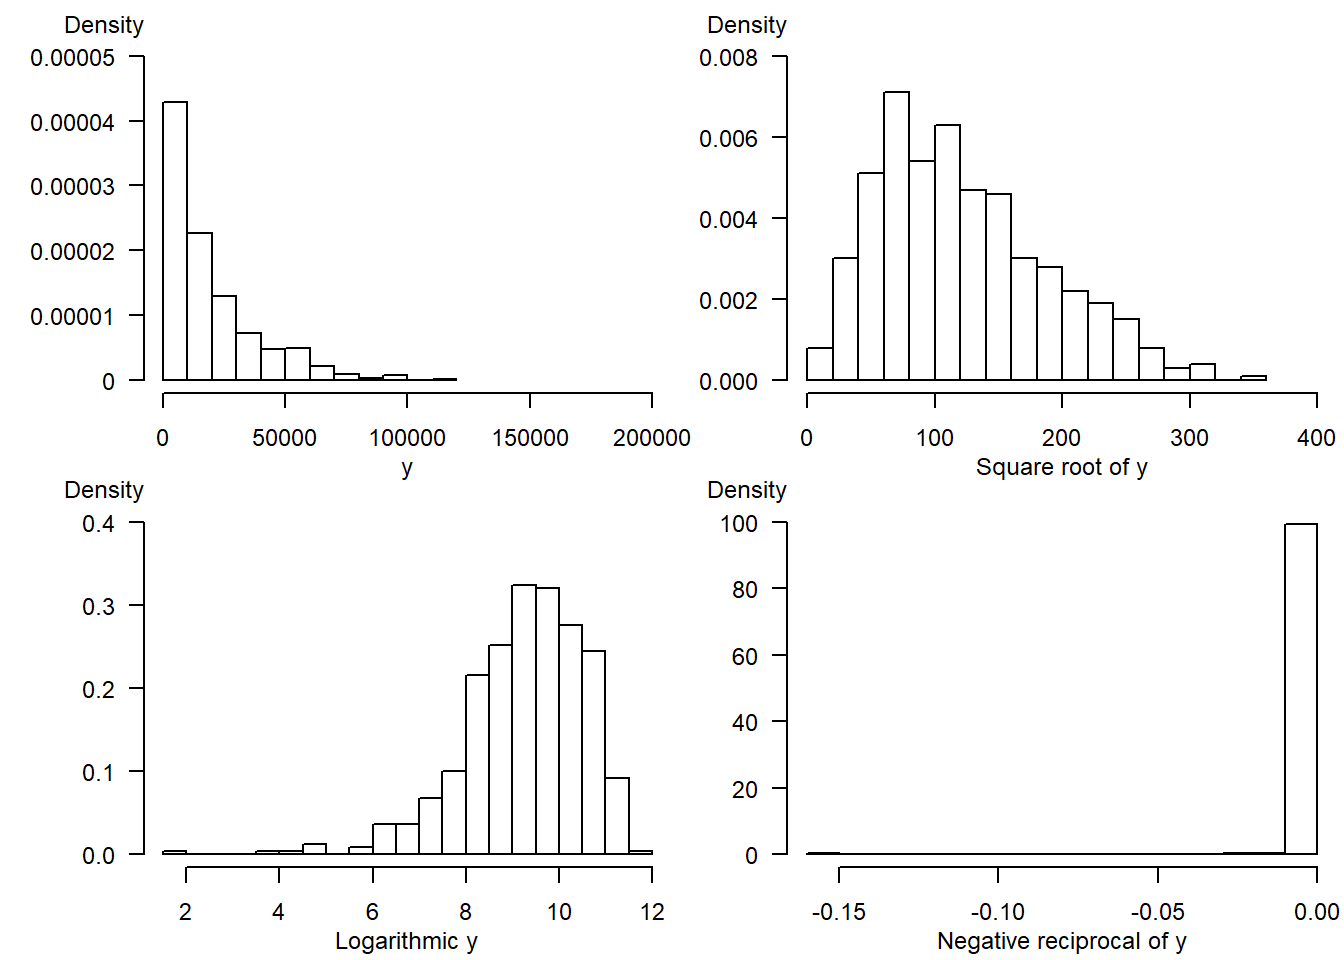
\includegraphics{RegressModelDataCamp_files/figure-latex/unnamed-chunk-38-1.pdf}

\subsection{Exercise. Distribution of transformed bodily injury
claims}\label{exercise.-distribution-of-transformed-bodily-injury-claims}

\textbf{Assignment Text}

We have now examined the distributions of bodily injury claims and its
logarithmic version. Grudgingly, we have concluded that to fit a normal
curve the logarithmic version of claims is a better choice (again, we
really do not like log dollars but you'll get used to it in this
course). But, why logarithmic and not some other transformations?

A partial response to this question will appear in later chapters when
we describe interpretation of regression coefficients. Another partial
response is that the log transform seems to work well with skewed
insurance data sets, as we demonstrate visually in this exercise.

\textbf{Instructions}

Use the code \texttt{par(mfrow\ =\ c(2,\ 2))} so that four graphs appear
in a 2 by 2 matrix format for easy comparisons. Plot the
\href{https://www.rdocumentation.org/packages/stats/versions/3.5.1/topics/density}{density()}
of

\begin{itemize}
\tightlist
\item
  claims
\item
  square root of claims
\item
  logarithmic claims
\item
  negative reciprocal of claims
\end{itemize}

\textbf{Hint.} For negative reciprocal claims, use
\texttt{plot(density(-claims\^{}(-1)))}

eyJsYW5ndWFnZSI6InIiLCJwcmVfZXhlcmNpc2VfY29kZSI6IiNpbmp1cnkgPC0gcmVhZC5jc3YoXCJDU1ZEYXRhXFxcXE1hc3NCSS5jc3ZcIiwgaGVhZGVyID0gVFJVRSlcbmluanVyeSA8LSByZWFkLmNzdihcImh0dHBzOi8vYXNzZXRzLmRhdGFjYW1wLmNvbS9wcm9kdWN0aW9uL3JlcG9zaXRvcmllcy8yNjEwL2RhdGFzZXRzLzhjY2ExOWQwNTAzZmNmNmU5ZDMwZDljYjkxMmRlNWJhOTVlY2I5YzEvTWFzc0JJLmNzdlwiLCBoZWFkZXIgPSBUUlVFKVxuY2xhaW1zIDwtIGluanVyeSRjbGFpbXMiLCJzYW1wbGUiOiIjVGhpcyBjb2RlIGhlbHBzIHRvIG9yZ2FuaXplIHRoZSBmb3VyIGdyYXBocyBpbnRvIGEgMiBieSAyIGZvcm1hdFxucGFyKG1mcm93ID0gYygyLCAyKSlcbiNQbG90IHRoZSBkZW5zaXR5IG9mIGNsYWltc1xucGxvdChkZW5zaXR5KF9fXykpXG5cbiNQbG90IHRoZSBkZW5zaXR5IG9mIHNxdWFyZSByb290IG9mIGNsYWltc1xucGxvdChkZW5zaXR5KF9fXykpIFxuXG4jUGxvdCB0aGUgZGVuc2l0eSBvZiBsb2dhcml0aG1pYyBjbGFpbXNcbnBsb3QoZGVuc2l0eShfX18pKVxuXG4jUGxvdCB0aGUgZGVuc2l0eSBvZiB0aGUgbmVnYXRpdmUgcmVjaXByb2NhbCBvZiBjbGFpbXNcbnBsb3QoZGVuc2l0eShfX18pKSIsInNvbHV0aW9uIjoicGFyKG1mcm93ID0gYygyLCAyKSlcbnBsb3QoZGVuc2l0eShjbGFpbXMpKSAgICBcbnBsb3QoZGVuc2l0eShjbGFpbXNeKDAuNSkpKSAgXG5wbG90KGRlbnNpdHkobG9nKGNsYWltcykpKSAgXG5wbG90KGRlbnNpdHkoLWNsYWltc14oLTEpKSkgICIsInNjdCI6InN1Y2Nlc3NfbXNnKFwiRXhjZWxsZW50ISBUcmFuc2Zvcm1hdGlvbnMgb2YgZGF0YSBpcyBhIHRvb2wgdGhhdCBpbmNyZWRpYmx5IGV4cGFuZHMgcG90ZW50aWFsIGFwcGxpY2FiaWxpdHkgb2YgKGxpbmVhcikgcmVncmVzc2lvbiB0ZWNobmlxdWVzLlwiKSJ9

\chapter{Basic Linear Regression}\label{basic-linear-regression}

\textbf{Chapter description}

This chapter considers regression in the case of only one explanatory
variable. Despite this seeming simplicity, many deep ideas of regression
can be developed in this framework. By limiting ourselves to the one
variable case, we can illustrate the relationships between two variables
graphically. Graphical tools prove to be important for developing a link
between the data and a predictive model.

\begin{Shaded}
\begin{Highlighting}[]
\CommentTok{# Reformat Data}
\NormalTok{Lot <-}\StringTok{ }\KeywordTok{read.table}\NormalTok{(}\StringTok{"CSVData}\CharTok{\textbackslash{}\textbackslash{}}\StringTok{WiscLottery.csv"}\NormalTok{,}\DataTypeTok{header =} \OtherTok{TRUE}\NormalTok{, }\DataTypeTok{sep =} \StringTok{","}\NormalTok{)}
\KeywordTok{str}\NormalTok{(Lot)}
\KeywordTok{cor}\NormalTok{(Lot)}
\NormalTok{Lot}\OperatorTok{$}\NormalTok{pop <-}\StringTok{ }\NormalTok{Lot}\OperatorTok{$}\NormalTok{POP}
\NormalTok{Lot}\OperatorTok{$}\NormalTok{sales <-}\StringTok{ }\NormalTok{Lot}\OperatorTok{$}\NormalTok{SALES}
\NormalTok{Lot}\OperatorTok{$}\NormalTok{medhome <-}\StringTok{ }\NormalTok{Lot}\OperatorTok{$}\NormalTok{MEDHVL}
\NormalTok{Lot2 <-}\StringTok{ }\NormalTok{Lot[}\KeywordTok{c}\NormalTok{(}\StringTok{"pop"}\NormalTok{,}\StringTok{"sales"}\NormalTok{,}\StringTok{"medhome"}\NormalTok{)]}
\CommentTok{#write.csv(Lot2,"CSVData\textbackslash{}\textbackslash{}Wisc_lottery.csv",row.names = FALSE)}


\NormalTok{outlr <-}\StringTok{ }\KeywordTok{read.csv}\NormalTok{(}\StringTok{"CSVData}\CharTok{\textbackslash{}\textbackslash{}}\StringTok{OutlierExample.csv"}\NormalTok{, }\DataTypeTok{header =} \OtherTok{TRUE}\NormalTok{)}
\KeywordTok{str}\NormalTok{(outlr)}
\NormalTok{outlr}\OperatorTok{$}\NormalTok{y <-}\StringTok{ }\NormalTok{outlr}\OperatorTok{$}\NormalTok{Y }
\NormalTok{outlr}\OperatorTok{$}\NormalTok{x <-}\StringTok{ }\NormalTok{outlr}\OperatorTok{$}\NormalTok{X}
\NormalTok{outlr}\OperatorTok{$}\NormalTok{codes <-}\StringTok{ }\NormalTok{outlr}\OperatorTok{$}\NormalTok{CODES}
\NormalTok{outlr2 <-}\StringTok{ }\NormalTok{outlr[}\KeywordTok{c}\NormalTok{(}\StringTok{"x"}\NormalTok{,}\StringTok{"y"}\NormalTok{,}\StringTok{"codes"}\NormalTok{)]}
\CommentTok{#write.csv(outlr2,"CSVData\textbackslash{}\textbackslash{}Outlier.csv",row.names = FALSE)}
\end{Highlighting}
\end{Shaded}

\section{Correlation}\label{correlation}

\subsection{Video (Exercise).
Correlation}\label{video-exercise.-correlation}

\subsubsection{Learning Objectives}\label{learning-objectives}

In this module, you learn how to:

\begin{itemize}
\tightlist
\item
  Calculate and interpret a correlation coefficient
\item
  Interpret correlation coefficients by visualizing scatter plots
\end{itemize}

\subsubsection{Video Overheads}\label{video-overheads}

\textbf{Overhead A. Wisconsin lottery data description}

\begin{Shaded}
\begin{Highlighting}[]
\NormalTok{Lot <-}\StringTok{ }\KeywordTok{read.csv}\NormalTok{(}\StringTok{"CSVData}\CharTok{\textbackslash{}\textbackslash{}}\StringTok{Wisc_lottery.csv"}\NormalTok{)}
\CommentTok{#Lot <- read.csv("https://assets.datacamp.com/production/repositories/2610/datasets/a792b30fb32b0896dd6894501cbab32b5d48df51/Wisc_lottery.csv", header = TRUE)}
\KeywordTok{str}\NormalTok{(Lot)}
\end{Highlighting}
\end{Shaded}

\textbf{Overhead B. Summary statistics}

\begin{Shaded}
\begin{Highlighting}[]
\CommentTok{#options(scipen = 100, digits = 4)}
\CommentTok{#numSummary(Lot[,c("pop", "sales")], statistics = c("mean", "sd", "quantiles"), quantiles = c(0,.5,1))}
\NormalTok{(}\KeywordTok{as.data.frame}\NormalTok{(psych}\OperatorTok{::}\KeywordTok{describe}\NormalTok{(Lot)))[,}\KeywordTok{c}\NormalTok{(}\DecValTok{2}\NormalTok{,}\DecValTok{3}\NormalTok{,}\DecValTok{4}\NormalTok{,}\DecValTok{5}\NormalTok{,}\DecValTok{8}\NormalTok{,}\DecValTok{9}\NormalTok{)]}
\CommentTok{#Rcmdr::numSummary(Lot[,c("pop", "sales")], statistics = c("mean", "sd", "quantiles"), quantiles = c(0,.5,1))}
\end{Highlighting}
\end{Shaded}

\textbf{Overhead C. Visualizing skewed distributions}

\begin{Shaded}
\begin{Highlighting}[]
\KeywordTok{par}\NormalTok{(}\DataTypeTok{mfrow =} \KeywordTok{c}\NormalTok{(}\DecValTok{1}\NormalTok{, }\DecValTok{2}\NormalTok{))}
\KeywordTok{hist}\NormalTok{(Lot}\OperatorTok{$}\NormalTok{pop, }\DataTypeTok{main =} \StringTok{""}\NormalTok{, }\DataTypeTok{xlab =} \StringTok{"population"}\NormalTok{)}
\KeywordTok{hist}\NormalTok{(Lot}\OperatorTok{$}\NormalTok{sales, }\DataTypeTok{main =} \StringTok{""}\NormalTok{, }\DataTypeTok{xlab =} \StringTok{"sales"}\NormalTok{)}
\end{Highlighting}
\end{Shaded}

\textbf{Overhead D. Visualizing relationships with a scatter plot}

\begin{Shaded}
\begin{Highlighting}[]
\KeywordTok{plot}\NormalTok{(Lot}\OperatorTok{$}\NormalTok{pop, Lot}\OperatorTok{$}\NormalTok{sales, }\DataTypeTok{xlab =} \StringTok{"population"}\NormalTok{, }\DataTypeTok{ylab =} \StringTok{"sales"}\NormalTok{)}
\end{Highlighting}
\end{Shaded}

\textbf{Overhead E. Correlation coefficient}

\begin{Shaded}
\begin{Highlighting}[]
\KeywordTok{cor}\NormalTok{(Lot}\OperatorTok{$}\NormalTok{pop, Lot}\OperatorTok{$}\NormalTok{sales)}
\end{Highlighting}
\end{Shaded}

\subsection{Exercise. Correlations and the Wisconsin
lottery}\label{exercise.-correlations-and-the-wisconsin-lottery}

\textbf{Assignment Text}

The Wisconsin lottery dataset, \texttt{Wisc\_lottery},has already been
read into a dataframe \texttt{Lot}.

Like insurance, lotteries are uncertain events and so the skills to work
with and interpret lottery data are readily applicable to insurance. It
is common to report sales and population in thousands of units, so this
exercise gives you practice in rescaling data via linear
transformations.

\textbf{Instructions}

\begin{itemize}
\tightlist
\item
  From the available population and sales variables, create new
  variables in the dataframe \texttt{Lot}, \texttt{pop\_1000} and
  \texttt{sales\_1000} that are in thousands (of people and of dollars,
  respectively).
\item
  Create summary statistics for the dataframe that includes these new
  variables.
\item
  Plot \texttt{pop\_1000} versus \texttt{sales\_1000}.
\item
  Calculate the correlation between \texttt{pop\_1000} versus
  \texttt{sales\_1000} using the function
  \href{https://www.rdocumentation.org/packages/stats/versions/3.5.0/topics/cor}{cor()}.
  How does this differ between the correlation between population and
  sales in the original units?
\end{itemize}

\textbf{Hint}

Use the dataframe to refer to pop and sales as \texttt{Lot\$pop} and
\texttt{Lot\$sales}, respectively

\textbf{Pre-exercise code}

\begin{Shaded}
\begin{Highlighting}[]
\CommentTok{# Pre-exercise code}
\CommentTok{#library(Rcmdr)}
\CommentTok{#library(psych)}
\NormalTok{Lot <-}\StringTok{ }\KeywordTok{read.csv}\NormalTok{(}\StringTok{"CSVData}\CharTok{\textbackslash{}\textbackslash{}}\StringTok{Wisc_lottery.csv"}\NormalTok{, }\DataTypeTok{header =} \OtherTok{TRUE}\NormalTok{)}
\CommentTok{#Lot <- read.csv("https://assets.datacamp.com/production/repositories/2610/datasets/a792b30fb32b0896dd6894501cbab32b5d48df51/Wisc_lottery.csv", header = TRUE)}
\end{Highlighting}
\end{Shaded}

\textbf{Sample\_code}

\begin{Shaded}
\begin{Highlighting}[]
\StringTok{`}\DataTypeTok{@Sample_code}\StringTok{`}
\CommentTok{# Create new variables, say, `pop_1000` and `sales_1000`}
\NormalTok{Lot}\OperatorTok{$}\NormalTok{pop_}\DecValTok{1000}\NormalTok{ <-}\StringTok{ }\NormalTok{___}
\NormalTok{___ <-}\StringTok{ }\NormalTok{Lot}\OperatorTok{$}\NormalTok{sales}\OperatorTok{/}\DecValTok{1000}

\CommentTok{# Create summary statistics for the dataframe}
\KeywordTok{summary}\NormalTok{(___)}

\CommentTok{# Plot `pop_1000` versus `sales_1000`.}
\KeywordTok{plot}\NormalTok{(___, ___)}

\CommentTok{# Calculate the correlation between `pop_1000` versus `sales_1000` }
\KeywordTok{cor}\NormalTok{(___, ___)}
\end{Highlighting}
\end{Shaded}

\textbf{Solution}

\begin{Shaded}
\begin{Highlighting}[]
\CommentTok{# Solution}
\NormalTok{Lot}\OperatorTok{$}\NormalTok{pop_}\DecValTok{1000}\NormalTok{ <-}\StringTok{ }\NormalTok{Lot}\OperatorTok{$}\NormalTok{pop}\OperatorTok{/}\DecValTok{1000}
\NormalTok{Lot}\OperatorTok{$}\NormalTok{sales_}\DecValTok{1000}\NormalTok{ <-}\StringTok{ }\NormalTok{Lot}\OperatorTok{$}\NormalTok{sales}\OperatorTok{/}\DecValTok{1000}
\KeywordTok{summary}\NormalTok{(Lot)}
\CommentTok{#(as.data.frame(psych::describe(Lot)))[,c(2,3,4,5,8,9)]}
\CommentTok{#(as.data.frame(psych::describe(Lot[,c("pop_1000", "sales_1000")])))[,c(2,3,4,5,8,9)]}
\CommentTok{#Rcmdr::numSummary(Lot[,c("pop_1000", "sales_1000")], statistics = c("mean", "sd", "quantiles"), quantiles = c(0,.5,1))}
\KeywordTok{plot}\NormalTok{(Lot}\OperatorTok{$}\NormalTok{pop_}\DecValTok{1000}\NormalTok{, Lot}\OperatorTok{$}\NormalTok{sales_}\DecValTok{1000}\NormalTok{)}
\KeywordTok{cor}\NormalTok{(Lot}\OperatorTok{$}\NormalTok{pop_}\DecValTok{1000}\NormalTok{, Lot}\OperatorTok{$}\NormalTok{sales_}\DecValTok{1000}\NormalTok{)}
\end{Highlighting}
\end{Shaded}

\textbf{Submission Correctness Tests (SCT)}

test\_error() test\_object(``Lot'', incorrect\_msg = ``Looks like a
variable is defined incorrectly. The hint may help.'')
success\_msg(``Congratulations! We will rescale data using `linear'
transformations regularly. In part we do this for communicating our
analysis to others. Also in part, this is for our own convenience as it
can allow us to see patterns more readily.'')

\section{Method of least squares}\label{method-of-least-squares}

\subsection{Video (Exercise). Method of least
squares}\label{video-exercise.-method-of-least-squares}

\subsubsection{Learning Objectives}\label{learning-objectives-1}

In this module, you learn how to:

\begin{itemize}
\tightlist
\item
  Fit a line to data using the method of least squares
\item
  Predict an observation using a least squares fitted line
\end{itemize}

\subsubsection{Video Overheads}\label{video-overheads-1}

\textbf{Overhead A. Where to fit the line?}

\begin{Shaded}
\begin{Highlighting}[]
\NormalTok{model_blr <-}\StringTok{ }\KeywordTok{lm}\NormalTok{(sales }\OperatorTok{~}\StringTok{ }\NormalTok{pop, }\DataTypeTok{data =}\NormalTok{ Lot)}
\KeywordTok{plot}\NormalTok{(Lot}\OperatorTok{$}\NormalTok{pop, Lot}\OperatorTok{$}\NormalTok{sales,}\DataTypeTok{xlab =} \StringTok{"population"}\NormalTok{, }\DataTypeTok{ylab =} \StringTok{"sales"}\NormalTok{)}
\KeywordTok{abline}\NormalTok{(model_blr, }\DataTypeTok{col=}\StringTok{"blue"}\NormalTok{)}
\KeywordTok{abline}\NormalTok{(}\DecValTok{0}\NormalTok{,}\DecValTok{1}\NormalTok{, }\DataTypeTok{col=}\StringTok{"red"}\NormalTok{)}
\end{Highlighting}
\end{Shaded}

\textbf{Overhead B. Method of least squares}

\begin{itemize}
\tightlist
\item
  For observation \(\{(y, x)\}\), the height of the regression line is
  \[b_0 + b_1 x.\]
\item
  Thus, \(y - (b_0 + b_1 x)\) represents the deviation.
\item
  The sum of squared deviations is
  \[SS(b_0, b_1) = \sum (y - (b_0 + b_1 x))^2 .\]
\item
  The \emph{method of least squares} -- determine values of \(b_0, b_1\)
  that minimize \(SS\).
\end{itemize}

\textbf{Overhead C. Regression coefficients}

\begin{Shaded}
\begin{Highlighting}[]
\NormalTok{model_blr <-}\StringTok{ }\KeywordTok{lm}\NormalTok{(sales }\OperatorTok{~}\StringTok{ }\NormalTok{pop, }\DataTypeTok{data =}\NormalTok{ Lot)}
\KeywordTok{round}\NormalTok{(}\KeywordTok{coefficients}\NormalTok{(model_blr), }\DataTypeTok{digits=}\DecValTok{4}\NormalTok{)}
\KeywordTok{plot}\NormalTok{(Lot}\OperatorTok{$}\NormalTok{pop, Lot}\OperatorTok{$}\NormalTok{sales,}\DataTypeTok{xlab =} \StringTok{"population"}\NormalTok{, }\DataTypeTok{ylab =} \StringTok{"sales"}\NormalTok{)}
\KeywordTok{abline}\NormalTok{(model_blr, }\DataTypeTok{col=}\StringTok{"blue"}\NormalTok{)}
\end{Highlighting}
\end{Shaded}

\textbf{Overhead D. Prediction}

\begin{Shaded}
\begin{Highlighting}[]
\KeywordTok{round}\NormalTok{(}\KeywordTok{coefficients}\NormalTok{(model_blr), }\DataTypeTok{digits=}\DecValTok{6}\NormalTok{)}
\KeywordTok{coefficients}\NormalTok{(model_blr)[}\DecValTok{1}\NormalTok{] }\OperatorTok{+}\StringTok{ }\KeywordTok{coefficients}\NormalTok{(model_blr)[}\DecValTok{2}\NormalTok{]}\OperatorTok{*}\DecValTok{30000}

\NormalTok{newdata <-}\StringTok{ }\KeywordTok{data.frame}\NormalTok{(}\DataTypeTok{pop =} \DecValTok{30000}\NormalTok{)}
\KeywordTok{predict}\NormalTok{(model_blr, newdata)}
\end{Highlighting}
\end{Shaded}

\subsection{Exercise. Least squares fit using housing
prices}\label{exercise.-least-squares-fit-using-housing-prices}

\textbf{Assignment Text}

The prior video analyzed the effect that a zip code's population has on
lottery sales. Instead of population, suppose that you wish to
understand the effect that housing prices have on the sale of lottery
tickets. The dataframe \texttt{Lot}, read in from the Wisconsin lottery
dataset \texttt{Wisc\_lottery}, contains the variable \texttt{medhome}
which is the median house price for each zip code, in thousands of
dollars. In this exercise, you will get a feel for the distribution of
this variable by examining summary statistics, examine its relationship
with sales graphically and via correlations, fit a basic linear
regression model and use this model to predict sales.

\textbf{Instructions}

\begin{itemize}
\tightlist
\item
  Summarize the dataframe \texttt{Lot} that contains \texttt{medhome}
  and \texttt{sales}.
\item
  Plot \texttt{medhome} versus \texttt{sales}. Summarize this
  relationship by calculating the corresponding correlation coefficient
  using the function
  \href{https://www.rdocumentation.org/packages/stats/versions/3.5.0/topics/cor}{cor()}.
\item
  Using the function
  \href{https://www.rdocumentation.org/packages/stats/versions/3.5.0/topics/lm}{lm()},
  regress \texttt{medhome}, the explanatory variable, on \texttt{sales},
  the outcome variable. Display the regression coefficients to four
  significant digits.
\item
  Use the function
  \href{https://www.rdocumentation.org/packages/stats/versions/3.5.0/topics/predict}{predict()}
  and the fitted regression model to predict sales assuming that the
  median house price for a zip code is 50 (in thousands of dollars).
\end{itemize}

\textbf{Hint}

\textbf{Pre-exercise code}

\begin{Shaded}
\begin{Highlighting}[]
\CommentTok{# Pre-exercise code}
\CommentTok{#library(Rcmdr)}
\NormalTok{Lot <-}\StringTok{ }\KeywordTok{read.csv}\NormalTok{(}\StringTok{"CSVData}\CharTok{\textbackslash{}\textbackslash{}}\StringTok{Wisc_lottery.csv"}\NormalTok{, }\DataTypeTok{header =} \OtherTok{TRUE}\NormalTok{)}
\CommentTok{#Lot <- read.csv("https://assets.datacamp.com/production/repositories/2610/datasets/a792b30fb32b0896dd6894501cbab32b5d48df51/Wisc_lottery.csv", header = TRUE)}
\end{Highlighting}
\end{Shaded}

\textbf{Sample\_code}

\begin{Shaded}
\begin{Highlighting}[]
\StringTok{`}\DataTypeTok{@Sample_code}\StringTok{`}
\CommentTok{# Summarize the dataframe `Lot` that contains `medhome` and `sales`}
\KeywordTok{summary}\NormalTok{(Lot)}
\CommentTok{# Plot and calculate the correlation of `medhome` versus `sales`. }
\KeywordTok{cor}\NormalTok{(___, ___)}
\KeywordTok{plot}\NormalTok{(___, ___)}

\CommentTok{# Regress `medhome`  on `sales`. Display the regression coefficients to four significant digits.}
\NormalTok{model_blr1 <-}\StringTok{ }\KeywordTok{lm}\NormalTok{(___ }\OperatorTok{~}\StringTok{ }\NormalTok{___, }\DataTypeTok{data =}\NormalTok{ Lot)}
\KeywordTok{round}\NormalTok{(}\KeywordTok{coefficients}\NormalTok{(model_blr1), }\DataTypeTok{digits=} \OperatorTok{---}\NormalTok{)}

\CommentTok{# Predict sales assuming that the median house price is 50 }
\NormalTok{newdata <-}\StringTok{ }\KeywordTok{data.frame}\NormalTok{(}\DataTypeTok{medhome =}\NormalTok{ ___)}
\KeywordTok{predict}\NormalTok{(model_blr1, newdata)}
\end{Highlighting}
\end{Shaded}

\textbf{Solution}

\begin{Shaded}
\begin{Highlighting}[]
\CommentTok{# Solution}
\CommentTok{#numSummary(Lot[,c("medhome", "sales")], statistics = c("mean", "sd", "quantiles"), quantiles = c(0,.5,1))}
\CommentTok{#(as.data.frame(psych::describe(Lot[,c("medhome", "sales")])))[,c(2,3,4,5,8,9)]}
\KeywordTok{summary}\NormalTok{(Lot)}
\KeywordTok{cor}\NormalTok{(Lot}\OperatorTok{$}\NormalTok{medhome,Lot}\OperatorTok{$}\NormalTok{sales)}
\KeywordTok{plot}\NormalTok{(Lot}\OperatorTok{$}\NormalTok{medhome,Lot}\OperatorTok{$}\NormalTok{sales)}
\NormalTok{model_blr1 <-}\StringTok{ }\KeywordTok{lm}\NormalTok{(sales }\OperatorTok{~}\StringTok{ }\NormalTok{medhome, }\DataTypeTok{data =}\NormalTok{ Lot)}
\KeywordTok{round}\NormalTok{(}\KeywordTok{coefficients}\NormalTok{(model_blr1), }\DataTypeTok{digits=}\DecValTok{4}\NormalTok{)}
\NormalTok{newdata <-}\StringTok{ }\KeywordTok{data.frame}\NormalTok{(}\DataTypeTok{medhome =} \DecValTok{50}\NormalTok{)}
\KeywordTok{predict}\NormalTok{(model_blr1, newdata)}
\end{Highlighting}
\end{Shaded}

\textbf{Submission Correctness Tests (SCT)}

test\_error() test\_object(``model\_blr1'', incorrect\_msg = ``The basic
linear regression model is incorrectly specified.'')
test\_object(``newdata'', incorrect\_msg = ``The new data is incorrectly
specified.'') success\_msg(``Congratulations! You now have experience
fitting a regression line and using this line for predictions, just as
Galton did when he used parents' heights to predict the height of an
adult child. Well done!'')

\section{Understanding variability}\label{understanding-variability}

\subsection{Video (Exercise). Understanding
variability}\label{video-exercise.-understanding-variability}

\subsubsection{Learning Objectives}\label{learning-objectives-2}

In this module, you learn how to:

\begin{itemize}
\tightlist
\item
  Visualize the ANOVA decomposition of variability
\item
  Calculate and interpret \(R^2\), the coefficient of determination
\item
  Calculate and interpret \(s^2\) the mean square error
\item
  Explain the components of the ANOVA table
\end{itemize}

\subsubsection{Video Overheads}\label{video-overheads-2}

\textbf{Overhead A. Visualizing the uncertainty about a line}

\textbf{Overhead B. R script for visualizing the uncertainty about a
line}

\begin{Shaded}
\begin{Highlighting}[]
\KeywordTok{par}\NormalTok{(}\DataTypeTok{mar=}\KeywordTok{c}\NormalTok{(}\FloatTok{2.2}\NormalTok{,}\FloatTok{2.1}\NormalTok{,.}\DecValTok{2}\NormalTok{,.}\DecValTok{2}\NormalTok{),}\DataTypeTok{cex=}\FloatTok{1.2}\NormalTok{)}
\NormalTok{x <-}\StringTok{ }\KeywordTok{seq}\NormalTok{(}\OperatorTok{-}\DecValTok{4}\NormalTok{, }\DecValTok{4}\NormalTok{, }\DataTypeTok{len=}\DecValTok{101}\NormalTok{)}
\NormalTok{y <-}\StringTok{ }\NormalTok{x}
\KeywordTok{plot}\NormalTok{(x, y, }\DataTypeTok{type =} \StringTok{"l"}\NormalTok{, }\DataTypeTok{xlim=}\KeywordTok{c}\NormalTok{(}\OperatorTok{-}\DecValTok{3}\NormalTok{, }\DecValTok{4}\NormalTok{), }\DataTypeTok{xaxt=}\StringTok{"n"}\NormalTok{, }\DataTypeTok{yaxt=}\StringTok{"n"}\NormalTok{, }\DataTypeTok{xlab=}\StringTok{""}\NormalTok{, }\DataTypeTok{ylab=}\StringTok{""}\NormalTok{)}
\KeywordTok{axis}\NormalTok{(}\DecValTok{1}\NormalTok{, }\DataTypeTok{at =} \KeywordTok{c}\NormalTok{(}\OperatorTok{-}\DecValTok{1}\NormalTok{, }\DecValTok{1}\NormalTok{),}\DataTypeTok{lab =} \KeywordTok{expression}\NormalTok{(}\KeywordTok{bar}\NormalTok{(x), x))}
\KeywordTok{axis}\NormalTok{(}\DecValTok{2}\NormalTok{, }\DataTypeTok{at =} \KeywordTok{c}\NormalTok{(}\OperatorTok{-}\DecValTok{1}\NormalTok{, }\DecValTok{1}\NormalTok{, }\DecValTok{3}\NormalTok{),}\DataTypeTok{lab =} \KeywordTok{expression}\NormalTok{(}\KeywordTok{bar}\NormalTok{(y), }\KeywordTok{hat}\NormalTok{(y), y), }\DataTypeTok{las=}\DecValTok{1}\NormalTok{)}
\KeywordTok{abline}\NormalTok{(}\OperatorTok{-}\DecValTok{1}\NormalTok{, }\DecValTok{0}\NormalTok{, }\DataTypeTok{lty =} \DecValTok{2}\NormalTok{)}
\KeywordTok{segments}\NormalTok{(}\OperatorTok{-}\DecValTok{4}\NormalTok{, }\DecValTok{1}\NormalTok{, }\DecValTok{1}\NormalTok{, }\DecValTok{1}\NormalTok{, }\DataTypeTok{lty=}\DecValTok{2}\NormalTok{)}
\KeywordTok{segments}\NormalTok{(}\OperatorTok{-}\DecValTok{4}\NormalTok{, }\DecValTok{3}\NormalTok{, }\DecValTok{1}\NormalTok{, }\DecValTok{3}\NormalTok{, }\DataTypeTok{lty =} \DecValTok{2}\NormalTok{)}
\KeywordTok{segments}\NormalTok{(}\DecValTok{1}\NormalTok{, }\OperatorTok{-}\DecValTok{4}\NormalTok{, }\DecValTok{1}\NormalTok{, }\DecValTok{3}\NormalTok{, }\DataTypeTok{lty =} \DecValTok{2}\NormalTok{)}
\KeywordTok{segments}\NormalTok{(}\OperatorTok{-}\DecValTok{1}\NormalTok{, }\OperatorTok{-}\DecValTok{4}\NormalTok{, }\OperatorTok{-}\DecValTok{1}\NormalTok{, }\OperatorTok{-}\DecValTok{1}\NormalTok{, }\DataTypeTok{lty =} \DecValTok{2}\NormalTok{)}

\KeywordTok{points}\NormalTok{(}\DecValTok{1}\NormalTok{, }\DecValTok{3}\NormalTok{, }\DataTypeTok{cex=}\FloatTok{1.5}\NormalTok{, }\DataTypeTok{pch=}\DecValTok{19}\NormalTok{)}

\KeywordTok{arrows}\NormalTok{(}\FloatTok{1.0}\NormalTok{, }\DecValTok{1}\NormalTok{, }\FloatTok{1.0}\NormalTok{, }\DecValTok{3}\NormalTok{, }\DataTypeTok{code =} \DecValTok{3}\NormalTok{, }\DataTypeTok{lty =} \DecValTok{1}\NormalTok{, }\DataTypeTok{angle=}\DecValTok{15}\NormalTok{, }\DataTypeTok{length=}\FloatTok{0.12}\NormalTok{, }\DataTypeTok{lwd=}\DecValTok{2}\NormalTok{)}
\KeywordTok{text}\NormalTok{(}\FloatTok{1.3}\NormalTok{, }\FloatTok{2.2}\NormalTok{,   }\KeywordTok{expression}\NormalTok{( y}\OperatorTok{-}\KeywordTok{hat}\NormalTok{(y)),}\DataTypeTok{cex=}\FloatTok{0.8}\NormalTok{) }
\KeywordTok{text}\NormalTok{(}\OperatorTok{-}\NormalTok{.}\DecValTok{3}\NormalTok{,}\FloatTok{2.2}\NormalTok{,}\StringTok{"'unexplained' deviation"}\NormalTok{, }\DataTypeTok{cex=}\NormalTok{.}\DecValTok{8}\NormalTok{) }
\KeywordTok{arrows}\NormalTok{(}\FloatTok{1.0}\NormalTok{, }\OperatorTok{-}\DecValTok{1}\NormalTok{, }\FloatTok{1.0}\NormalTok{, }\DecValTok{1}\NormalTok{, }\DataTypeTok{code =} \DecValTok{3}\NormalTok{, }\DataTypeTok{lty =} \DecValTok{1}\NormalTok{, }\DataTypeTok{angle=}\DecValTok{15}\NormalTok{, }\DataTypeTok{length=}\FloatTok{0.12}\NormalTok{, }\DataTypeTok{lwd=}\DecValTok{2}\NormalTok{)}
\KeywordTok{text}\NormalTok{(}\FloatTok{1.85}\NormalTok{, }\DecValTok{0}\NormalTok{, }\KeywordTok{expression}\NormalTok{(}\KeywordTok{hat}\NormalTok{(y)}\OperatorTok{-}\KeywordTok{bar}\NormalTok{(y) }\OperatorTok{==}\StringTok{ }\NormalTok{b[}\DecValTok{1}\NormalTok{](x}\OperatorTok{-}\KeywordTok{bar}\NormalTok{(x)) ), }\DataTypeTok{cex=}\FloatTok{0.8}\NormalTok{ )}
\KeywordTok{text}\NormalTok{(}\FloatTok{2.1}\NormalTok{, }\OperatorTok{-}\FloatTok{0.5}\NormalTok{, }\StringTok{" 'explained' deviation"}\NormalTok{, }\DataTypeTok{cex=}\FloatTok{0.8}\NormalTok{)}
\KeywordTok{arrows}\NormalTok{(}\OperatorTok{-}\DecValTok{1}\NormalTok{, }\OperatorTok{-}\FloatTok{1.0}\NormalTok{, }\DecValTok{1}\NormalTok{, }\OperatorTok{-}\FloatTok{1.0}\NormalTok{, }\DataTypeTok{code =} \DecValTok{3}\NormalTok{, }\DataTypeTok{lty =} \DecValTok{1}\NormalTok{, }\DataTypeTok{angle=}\DecValTok{15}\NormalTok{, }\DataTypeTok{length=}\FloatTok{0.12}\NormalTok{, }\DataTypeTok{lwd =} \DecValTok{2}\NormalTok{)}
\KeywordTok{text}\NormalTok{(}\DecValTok{0}\NormalTok{, }\OperatorTok{-}\FloatTok{1.3}\NormalTok{, }\KeywordTok{expression}\NormalTok{( x}\OperatorTok{-}\KeywordTok{bar}\NormalTok{(x)), }\DataTypeTok{cex=}\FloatTok{0.8}\NormalTok{  )}
\KeywordTok{text}\NormalTok{(}\FloatTok{3.5}\NormalTok{, }\FloatTok{2.7}\NormalTok{, }\KeywordTok{expression}\NormalTok{( }\KeywordTok{hat}\NormalTok{(y)}\OperatorTok{==}\StringTok{ }\NormalTok{b[}\DecValTok{0}\NormalTok{]}\OperatorTok{+}\StringTok{ }\NormalTok{b[}\DecValTok{1}\NormalTok{]}\OperatorTok{*}\NormalTok{x), }\DataTypeTok{cex=}\FloatTok{0.8}\NormalTok{  )}
\end{Highlighting}
\end{Shaded}

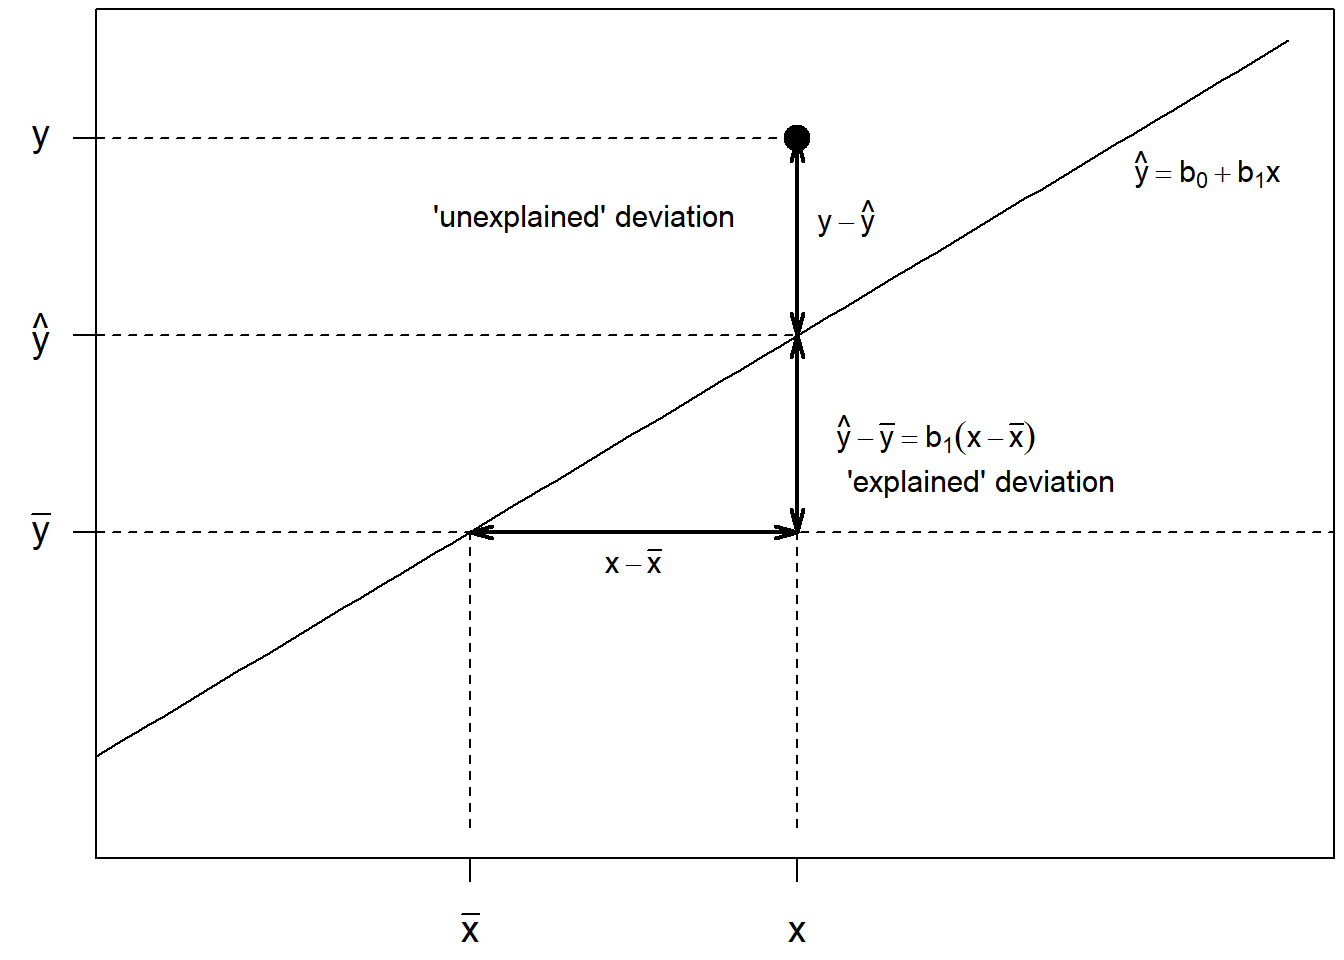
\includegraphics{RegressModelDataCamp_files/figure-latex/unnamed-chunk-58-1.pdf}

\textbf{Overhead C. The coefficient of determination, \(R^2\) }

\textbf{Overhead D. The mean square error, \(s^2\) }

\textbf{Overhead E. ANOVA Table}

\begin{Shaded}
\begin{Highlighting}[]
\NormalTok{model_blr <-}\StringTok{ }\KeywordTok{lm}\NormalTok{(sales }\OperatorTok{~}\StringTok{ }\NormalTok{pop, }\DataTypeTok{data =}\NormalTok{ Lot)}
\KeywordTok{anova}\NormalTok{(model_blr)}
\KeywordTok{sqrt}\NormalTok{(}\KeywordTok{anova}\NormalTok{(model_blr)}\OperatorTok{$}\NormalTok{Mean[}\DecValTok{2}\NormalTok{])}
\KeywordTok{summary}\NormalTok{(model_blr)}\OperatorTok{$}\NormalTok{r.squared}
\end{Highlighting}
\end{Shaded}

\subsection{Exercise. Summarizing measures of
uncertainty}\label{exercise.-summarizing-measures-of-uncertainty}

\textbf{Assignment Text}

In a previous exercise, you developed a regression line to fit the
variable \texttt{medhome}, the median house price for each zip code, as
a predictor of lottery sales. The regression of \texttt{medhome} on
\texttt{sales} has been summarized in the \texttt{R} object
\texttt{model\_blr}.

How reliable is the regression line? In this excercise, you will compute
some of the standard measures that are used to summarize the goodness of
this fit.

\textbf{Instructions}

\begin{itemize}
\tightlist
\item
  Summarize the fitted regression model in an ANOVA table.
\item
  Determine the size of the typical residual, \(s\).
\item
  Determine the coefficient of determination, \(R^2\).
\end{itemize}

\textbf{Hint}

Learn more about possibilities through the \texttt{Rdocumentation} site.
If you have not done so already, check out the function
\href{https://www.rdocumentation.org/packages/stats/versions/3.5.1/topics/anova}{anova()}

\textbf{Pre-exercise code}

\begin{Shaded}
\begin{Highlighting}[]
\CommentTok{# Pre-exercise code}
\NormalTok{Lot <-}\StringTok{ }\KeywordTok{read.csv}\NormalTok{(}\StringTok{"CSVData}\CharTok{\textbackslash{}\textbackslash{}}\StringTok{Wisc_lottery.csv"}\NormalTok{, }\DataTypeTok{header =} \OtherTok{TRUE}\NormalTok{)}
\CommentTok{#Lot <- read.csv("https://assets.datacamp.com/production/repositories/2610/datasets/a792b30fb32b0896dd6894501cbab32b5d48df51/Wisc_lottery.csv", header = TRUE)}
\end{Highlighting}
\end{Shaded}

\textbf{Sample\_code}

\begin{Shaded}
\begin{Highlighting}[]
\StringTok{`}\DataTypeTok{@Sample_code}\StringTok{`}
\NormalTok{model_blr <-}\StringTok{ }\KeywordTok{lm}\NormalTok{(sales  }\OperatorTok{~}\StringTok{ }\NormalTok{medhome, }\DataTypeTok{data =}\NormalTok{ Lot)}

\CommentTok{# Summarize the fitted regression model in an ANOVA table.}
\KeywordTok{anova}\NormalTok{(___)}

\CommentTok{# Determine the size of the typical residual, $s$.}
\KeywordTok{sqrt}\NormalTok{(}\KeywordTok{anova}\NormalTok{(___)}\OperatorTok{$}\NormalTok{Mean[}\DecValTok{2}\NormalTok{])}

\CommentTok{# Determine the coefficient of determination, $R^2$. }
\KeywordTok{summary}\NormalTok{(___)}\OperatorTok{$}\NormalTok{r.squared}
\end{Highlighting}
\end{Shaded}

\textbf{Solution}

\begin{Shaded}
\begin{Highlighting}[]
\CommentTok{# Solution}
\NormalTok{model_blr <-}\StringTok{ }\KeywordTok{lm}\NormalTok{(sales  }\OperatorTok{~}\StringTok{ }\NormalTok{medhome, }\DataTypeTok{data =}\NormalTok{ Lot)}
\KeywordTok{anova}\NormalTok{(model_blr)}
\KeywordTok{sqrt}\NormalTok{(}\KeywordTok{anova}\NormalTok{(model_blr)}\OperatorTok{$}\NormalTok{Mean[}\DecValTok{2}\NormalTok{])}
\KeywordTok{summary}\NormalTok{(model_blr)}\OperatorTok{$}\NormalTok{r.squared}
\end{Highlighting}
\end{Shaded}

\textbf{Submission Correctness Tests (SCT)}

test\_error() test\_object(``model\_blr'', incorrect\_msg = ``The basic
linear regression model is incorrectly specified.'')
success\_msg(``Congratulations! It will be helpful if you compare the
results of this exercise to the regression of \texttt{pop} on
\texttt{sales} from the prior video. We have seen that \texttt{pop} is
more highly correlated with \texttt{sales} than \texttt{medhome}, so we
are expecting greater uncertainty in this regression fit.'')

\subsection{Exercise. Effects of linear transforms on measures of
uncertainty}\label{exercise.-effects-of-linear-transforms-on-measures-of-uncertainty}

\textbf{Assignment Text}

Let us see how rescaling, a linear transformation, affects our measures
of uncertainty. As before, the Wisconsin lottery dataset
\texttt{Wisc\_lottery} has been read into a dataframe \texttt{Lot} that
also contains \texttt{sales\_1000}, sales in thousands of dollars, and
\texttt{pop\_1000}, zip code population in thousands. How do measures of
uncertainty change when going from the original units to thousands of
those units?

\textbf{Instructions}

\begin{itemize}
\tightlist
\item
  Run a regression of \texttt{pop} on \texttt{sales\_1000} and summarize
  this in an ANOVA table.
\item
  For this regression, determine the \(s\) and the coefficient of
  determination, \(R^2\).\\
\item
  Run a regression of \texttt{pop\_1000} on \texttt{sales\_1000} and
  summarize this in an ANOVA table.
\item
  For this regression, determine the \(s\) and the coefficient of
  determination, \(R^2\).
\end{itemize}

\textbf{Hint}

The residual standard error is also available as
\texttt{summary(model\_blr1)\$sigma}. The coefficient of determination
is also available as \texttt{summary(model\_blr1)\$r.squared}.

\textbf{Pre-exercise code}

\begin{Shaded}
\begin{Highlighting}[]
\CommentTok{# Pre-exercise code}
\CommentTok{#library(Rcmdr)}
\NormalTok{Lot <-}\StringTok{ }\KeywordTok{read.csv}\NormalTok{(}\StringTok{"CSVData}\CharTok{\textbackslash{}\textbackslash{}}\StringTok{Wisc_lottery.csv"}\NormalTok{, }\DataTypeTok{header =} \OtherTok{TRUE}\NormalTok{)}
\CommentTok{#Lot <- read.csv("https://assets.datacamp.com/production/repositories/2610/datasets/a792b30fb32b0896dd6894501cbab32b5d48df51/Wisc_lottery.csv", header = TRUE)}
\NormalTok{Lot}\OperatorTok{$}\NormalTok{pop_}\DecValTok{1000}\NormalTok{ <-}\StringTok{ }\NormalTok{Lot}\OperatorTok{$}\NormalTok{pop}\OperatorTok{/}\DecValTok{1000}
\NormalTok{Lot}\OperatorTok{$}\NormalTok{sales_}\DecValTok{1000}\NormalTok{ <-}\StringTok{ }\NormalTok{Lot}\OperatorTok{$}\NormalTok{sales}\OperatorTok{/}\DecValTok{1000}
\end{Highlighting}
\end{Shaded}

\textbf{Sample\_code}

\begin{Shaded}
\begin{Highlighting}[]
\StringTok{`}\DataTypeTok{@Sample_code}\StringTok{`}
\CommentTok{# Run a regression of `pop` on `sales_1000` and summarize this in an ANOVA table.}
\NormalTok{model_blr1 <-}\StringTok{ }\KeywordTok{lm}\NormalTok{(sales_}\DecValTok{1000}  \OperatorTok{~}\StringTok{ }\NormalTok{pop, }\DataTypeTok{data =}\NormalTok{ Lot)}
\KeywordTok{anova}\NormalTok{(___)}

\CommentTok{# Determine the $s$ and the coefficient of determination, $R^2$.  }
\KeywordTok{sqrt}\NormalTok{(}\KeywordTok{anova}\NormalTok{(___)}\OperatorTok{$}\NormalTok{Mean[}\DecValTok{2}\NormalTok{])}
\KeywordTok{summary}\NormalTok{(___)}\OperatorTok{$}\NormalTok{r.squared}

\CommentTok{# Run a regression of `pop_1000` on `sales_1000` and summarize this in an ANOVA table.}
\NormalTok{model_blr2 <-}\StringTok{ }\KeywordTok{lm}\NormalTok{(___  }\OperatorTok{~}\StringTok{ }\NormalTok{___, }\DataTypeTok{data =}\NormalTok{ Lot)}
\KeywordTok{anova}\NormalTok{(model_blr2)}

\CommentTok{# Determine the $s$ and the coefficient of determination, $R^2$. }
\NormalTok{___}
\NormalTok{___}
\end{Highlighting}
\end{Shaded}

\textbf{Solution}

\begin{Shaded}
\begin{Highlighting}[]
\CommentTok{# Solution}
\NormalTok{model_blr1 <-}\StringTok{ }\KeywordTok{lm}\NormalTok{(sales_}\DecValTok{1000}  \OperatorTok{~}\StringTok{ }\NormalTok{pop, }\DataTypeTok{data =}\NormalTok{ Lot)}
\KeywordTok{anova}\NormalTok{(model_blr1)}
\KeywordTok{sqrt}\NormalTok{(}\KeywordTok{anova}\NormalTok{(model_blr1)}\OperatorTok{$}\NormalTok{Mean[}\DecValTok{2}\NormalTok{])}
\KeywordTok{summary}\NormalTok{(model_blr1)}\OperatorTok{$}\NormalTok{r.squared}
\NormalTok{model_blr2 <-}\StringTok{ }\KeywordTok{lm}\NormalTok{(sales_}\DecValTok{1000}  \OperatorTok{~}\StringTok{ }\NormalTok{pop_}\DecValTok{1000}\NormalTok{ , }\DataTypeTok{data =}\NormalTok{ Lot)}
\KeywordTok{anova}\NormalTok{(model_blr2)}
\KeywordTok{sqrt}\NormalTok{(}\KeywordTok{anova}\NormalTok{(model_blr2)}\OperatorTok{$}\NormalTok{Mean[}\DecValTok{2}\NormalTok{])}
\KeywordTok{summary}\NormalTok{(model_blr2)}\OperatorTok{$}\NormalTok{r.squared}
\end{Highlighting}
\end{Shaded}

\textbf{Submission Correctness Tests (SCT)}

test\_error() test\_object(``model\_blr1'', incorrect\_msg = ``The basic
linear regression model is incorrectly specified.'')
success\_msg(``Congratulations! In this exercise, you have seen that
rescaling does not affect our measures of goodness of fit in any
meaningful way. For example, the coefficient of determinations are
completely unaffected. This is helpful because we will rescale variables
extensively in our search for patterns in the data.'')

\section{Statistical inference}\label{statistical-inference}

\subsection{Video (Exercise). Statistical
inference}\label{video-exercise.-statistical-inference}

\subsubsection{Learning Objectives}\label{learning-objectives-3}

In this module, you learn how to:

\begin{itemize}
\tightlist
\item
  Conduct a hypothesis test for a regression coefficient using either a
  rejection/acceptance procedure or a p-value
\item
  Calculate and interpret a confidence interval for a regression
  coefficient
\item
  Calculate and interpret a prediction interval at a specific value of a
  predictor variable
\end{itemize}

\textbf{Overhead A. Summary of basic linear regression model}

Introduce the output in the \emph{summary} of the basic linear
regression model.

\begin{Shaded}
\begin{Highlighting}[]
\NormalTok{Lot <-}\StringTok{ }\KeywordTok{read.csv}\NormalTok{(}\StringTok{"CSVData}\CharTok{\textbackslash{}\textbackslash{}}\StringTok{Wisc_lottery.csv"}\NormalTok{, }\DataTypeTok{header =} \OtherTok{TRUE}\NormalTok{)}
\CommentTok{#Lot <- read.csv("https://assets.datacamp.com/production/repositories/2610/datasets/a792b30fb32b0896dd6894501cbab32b5d48df51/Wisc_lottery.csv", header = TRUE)}
\CommentTok{#options(scipen = 8, digits = 4)}
\NormalTok{model_blr <-}\StringTok{ }\KeywordTok{lm}\NormalTok{(sales }\OperatorTok{~}\StringTok{ }\NormalTok{pop, }\DataTypeTok{data =}\NormalTok{ Lot)}
\KeywordTok{summary}\NormalTok{(model_blr)}
\end{Highlighting}
\end{Shaded}

\textbf{Overhead B. Hypothesis testing}

\begin{verbatim}
> summary(model_blr)$coefficients
            Estimate Std. Error t value  Pr(>|t|)
(Intercept) 469.7036  702.90619  0.6682 5.072e-01
pop           0.6471    0.04881 13.2579 1.158e-17
\end{verbatim}

\textbf{Overhead C. Confidence intervals}

\begin{Shaded}
\begin{Highlighting}[]
\NormalTok{Rcmdr}\OperatorTok{::}\KeywordTok{Confint}\NormalTok{(model_blr, }\DataTypeTok{level =}\NormalTok{ .}\DecValTok{90}\NormalTok{)}
\NormalTok{Rcmdr}\OperatorTok{::}\KeywordTok{Confint}\NormalTok{(model_blr, }\DataTypeTok{level =}\NormalTok{ .}\DecValTok{95}\NormalTok{)}
\end{Highlighting}
\end{Shaded}

\textbf{Overhead D. Confidence intervals check}

\begin{Shaded}
\begin{Highlighting}[]
\CommentTok{# Just for checking}
\KeywordTok{summary}\NormalTok{(model_blr)}\OperatorTok{$}\NormalTok{coefficients[}\DecValTok{2}\NormalTok{,}\DecValTok{1}\NormalTok{]}
\KeywordTok{summary}\NormalTok{(model_blr)}\OperatorTok{$}\NormalTok{coefficients[}\DecValTok{2}\NormalTok{,}\DecValTok{2}\NormalTok{]}
\KeywordTok{qt}\NormalTok{(.}\DecValTok{975}\NormalTok{, }\DecValTok{48}\NormalTok{)}

\KeywordTok{summary}\NormalTok{(model_blr)}\OperatorTok{$}\NormalTok{coefficients[}\DecValTok{2}\NormalTok{,}\DecValTok{1}\NormalTok{] }\OperatorTok{-}\StringTok{ }
\StringTok{  }\KeywordTok{summary}\NormalTok{(model_blr)}\OperatorTok{$}\NormalTok{coefficients[}\DecValTok{2}\NormalTok{,}\DecValTok{2}\NormalTok{]}\OperatorTok{*}\KeywordTok{qt}\NormalTok{(.}\DecValTok{975}\NormalTok{, }\DecValTok{48}\NormalTok{)}

\NormalTok{Rcmdr}\OperatorTok{::}\KeywordTok{Confint}\NormalTok{(model_blr, }\DataTypeTok{level =}\NormalTok{ .}\DecValTok{95}\NormalTok{)}
\KeywordTok{confint}\NormalTok{(model_blr, }\DataTypeTok{level =}\NormalTok{ .}\DecValTok{95}\NormalTok{)}
\end{Highlighting}
\end{Shaded}

\textbf{Overhead E. Prediction intervals}

\begin{Shaded}
\begin{Highlighting}[]
\NormalTok{NewData <-}\StringTok{ }\KeywordTok{data.frame}\NormalTok{(}\DataTypeTok{pop =} \DecValTok{10000}\NormalTok{)}
\KeywordTok{predict}\NormalTok{(model_blr, NewData, }\DataTypeTok{interval =} \StringTok{"prediction"}\NormalTok{, }\DataTypeTok{level =}\NormalTok{ .}\DecValTok{90}\NormalTok{)}
\KeywordTok{predict}\NormalTok{(model_blr, NewData, }\DataTypeTok{interval =} \StringTok{"prediction"}\NormalTok{, }\DataTypeTok{level =}\NormalTok{ .}\DecValTok{99}\NormalTok{)}
\end{Highlighting}
\end{Shaded}

\subsection{Exercise. Statistical inference and Wisconsin
lottery}\label{exercise.-statistical-inference-and-wisconsin-lottery}

\textbf{Assignment Text}

In a previous exercise, you developed a regression line with the
variable \texttt{medhome}, the median house price for each zip code, as
a predictor of lottery sales. The regression of \texttt{medhome} on
\texttt{sales} has been summarized in the \texttt{R} object
\texttt{model\_blr}.

This exercise allows you to practice the standard inferential tasks:
hypothesis testing, confidence intervals, and prediction.

\textbf{Instructions}

\begin{itemize}
\tightlist
\item
  Summarize the regression model and identify the \emph{t}-statistic for
  testing the importance of the regression coefficient associated with
  \texttt{medhome}.
\item
  Use the function
  \href{https://www.rdocumentation.org/packages/stats/versions/3.5.0/topics/confint}{confint()}
  to provide a 95\% confidence interval for the regression coefficient
  associated with \texttt{medhome}.
\item
  Consider a zip code with a median housing price equal to 50 (in
  thousands of dollars). Use the function
  \href{https://www.rdocumentation.org/packages/stats/versions/3.5.0/topics/predict}{predict()}
  to provide a point prediction and a 95\% prediction interval for
  sales.
\end{itemize}

\textbf{Hint}

Taking a {[}summary(){]} of a regression object produces a new objeect.
You can use the {[}str(){]} structure command to learn more about the
new object. Try out a command such as \texttt{str(summary(model\_blr))}

\textbf{Pre-exercise code}

\begin{Shaded}
\begin{Highlighting}[]
\CommentTok{# Pre-exercise code}
\NormalTok{Lot <-}\StringTok{ }\KeywordTok{read.csv}\NormalTok{(}\StringTok{"CSVData}\CharTok{\textbackslash{}\textbackslash{}}\StringTok{Wisc_lottery.csv"}\NormalTok{, }\DataTypeTok{header =} \OtherTok{TRUE}\NormalTok{)}
\CommentTok{#Lot <- read.csv("https://assets.datacamp.com/production/repositories/2610/datasets/a792b30fb32b0896dd6894501cbab32b5d48df51/Wisc_lottery.csv", header = TRUE)}
\end{Highlighting}
\end{Shaded}

\textbf{Sample\_code}

\begin{Shaded}
\begin{Highlighting}[]
\StringTok{`}\DataTypeTok{@sample_code}\StringTok{`}
\NormalTok{model_blr1 <-}\StringTok{ }\KeywordTok{lm}\NormalTok{(sales }\OperatorTok{~}\StringTok{ }\NormalTok{medhome, }\DataTypeTok{data =}\NormalTok{ Lot)}
\CommentTok{# Summarize the regression model and identify the $t$-statistic for testing the importance of the regression coefficient associated with `medhome`.}
\KeywordTok{summary}\NormalTok{(___)}
\KeywordTok{summary}\NormalTok{(___)}\OperatorTok{$}\NormalTok{coefficients}
\KeywordTok{summary}\NormalTok{(___)}\OperatorTok{$}\NormalTok{coefficients[,}\DecValTok{3}\NormalTok{]}

\CommentTok{# Provide a 95\textbackslash{}% confidence interval for the regression coefficient associated with `medhome`.}
\KeywordTok{confint}\NormalTok{(___, }\DataTypeTok{level =}\NormalTok{ ___)}

\CommentTok{# Provide a point prediction and a 95\textbackslash{}% prediction interval for sales.}
\NormalTok{NewData1 <-}\StringTok{ }\KeywordTok{data.frame}\NormalTok{(}\DataTypeTok{medhome =} \DecValTok{50}\NormalTok{)}
\KeywordTok{predict}\NormalTok{(___, NewData1, }\DataTypeTok{interval =} \StringTok{"prediction"}\NormalTok{, }\DataTypeTok{level =}\NormalTok{ ___)}
\end{Highlighting}
\end{Shaded}

\textbf{Solution}

\begin{Shaded}
\begin{Highlighting}[]
\CommentTok{# Solution}
\NormalTok{model_blr1 <-}\StringTok{ }\KeywordTok{lm}\NormalTok{(sales }\OperatorTok{~}\StringTok{ }\NormalTok{medhome, }\DataTypeTok{data =}\NormalTok{ Lot)}
\KeywordTok{summary}\NormalTok{(model_blr1)}
\KeywordTok{summary}\NormalTok{(model_blr1)}\OperatorTok{$}\NormalTok{coefficients}
\KeywordTok{summary}\NormalTok{(model_blr1)}\OperatorTok{$}\NormalTok{coefficients[,}\DecValTok{3}\NormalTok{]}

\CommentTok{#Rcmdr::Confint(model_blr1, level = .95)}
\KeywordTok{confint}\NormalTok{(model_blr1, }\DataTypeTok{level =}\NormalTok{ .}\DecValTok{95}\NormalTok{)}

\NormalTok{NewData1 <-}\StringTok{ }\KeywordTok{data.frame}\NormalTok{(}\DataTypeTok{medhome =} \DecValTok{50}\NormalTok{)}
\KeywordTok{predict}\NormalTok{(model_blr1, NewData1, }\DataTypeTok{interval =} \StringTok{"prediction"}\NormalTok{, }\DataTypeTok{level =}\NormalTok{ .}\DecValTok{95}\NormalTok{)}
\end{Highlighting}
\end{Shaded}

\textbf{Submission Correctness Tests (SCT)}

test\_error() test\_object(``model\_blr1'', incorrect\_msg = ``The basic
linear regression model is incorrectly specified.'')
test\_object(``NewData1'', incorrect\_msg = ``The new data object is
incorrectly specified.'') success\_msg(``Congratulations! Much of what
we learn from a data modeling exercise can be summarized using standard
inferential tools: hypothesis testing, confidence intervals, and
prediction.'')

\section{Diagnostics}\label{diagnostics}

\subsection{Video (Exercise).
Diagnostics}\label{video-exercise.-diagnostics}

\subsubsection{Learning Objectives}\label{learning-objectives-4}

In this module, you learn how to:

\begin{itemize}
\tightlist
\item
  Describe how diagnostic checking and residual analysis are used in a
  statistical analysis
\item
  Describe several model misspecifications commonly encountered in a
  regression analysis
\end{itemize}

\textbf{Overhead A. Unusual observations in regression}

\begin{itemize}
\tightlist
\item
  We have defined regression estimates as minimizers of a least squares
  objective function.
\item
  An appealing intuitive feature of linear regressions is that
  regression estimates can be expressed as weighted averages of
  outcomes.
\item
  The weights vary by observation, some observations are more important
  than others.
\item
  ``Unusual'' observations are far from the majority of the data set:
\item
  Unusual in the vertical direction is called an \emph{outlier}.
\item
  Unusual in the horizontal directional is called a \emph{high leverage
  point}.
\end{itemize}

\textbf{Overhead B. Example. Outliers and High Leverage Points}

\begin{Shaded}
\begin{Highlighting}[]
\NormalTok{outlr <-}\StringTok{ }\KeywordTok{read.csv}\NormalTok{(}\StringTok{"CSVData}\CharTok{\textbackslash{}\textbackslash{}}\StringTok{Outlier.csv"}\NormalTok{, }\DataTypeTok{header =} \OtherTok{TRUE}\NormalTok{)}

\CommentTok{#  FIGURE 2.7}
\KeywordTok{plot}\NormalTok{(outlr}\OperatorTok{$}\NormalTok{x, outlr}\OperatorTok{$}\NormalTok{y, }\DataTypeTok{xlim =} \KeywordTok{c}\NormalTok{(}\DecValTok{0}\NormalTok{, }\DecValTok{10}\NormalTok{), }\DataTypeTok{ylim =} \KeywordTok{c}\NormalTok{(}\DecValTok{2}\NormalTok{, }\DecValTok{9}\NormalTok{), }\DataTypeTok{xlab =} \StringTok{"x"}\NormalTok{, }\DataTypeTok{ylab =} \StringTok{"y"}\NormalTok{)}
\KeywordTok{text}\NormalTok{(}\FloatTok{4.5}\NormalTok{, }\FloatTok{8.0}\NormalTok{, }\StringTok{"A"}\NormalTok{)}
\KeywordTok{text}\NormalTok{(}\FloatTok{9.8}\NormalTok{, }\FloatTok{8.0}\NormalTok{, }\StringTok{"B"}\NormalTok{)}
\KeywordTok{text}\NormalTok{(}\FloatTok{9.8}\NormalTok{, }\FloatTok{2.5}\NormalTok{, }\StringTok{"C"}\NormalTok{)}
\end{Highlighting}
\end{Shaded}

\textbf{Overhead C. Regression fit with 19 base observations}

\begin{Shaded}
\begin{Highlighting}[]
\NormalTok{model_outlr0 <-}\StringTok{ }\KeywordTok{lm}\NormalTok{(y }\OperatorTok{~}\StringTok{ }\NormalTok{x, }\DataTypeTok{data =}\NormalTok{ outlr, }\DataTypeTok{subset =} \OperatorTok{-}\KeywordTok{c}\NormalTok{(}\DecValTok{20}\NormalTok{,}\DecValTok{21}\NormalTok{,}\DecValTok{22}\NormalTok{))}
\KeywordTok{summary}\NormalTok{(model_outlr0)}
\KeywordTok{plot}\NormalTok{(outlr}\OperatorTok{$}\NormalTok{x[}\DecValTok{1}\OperatorTok{:}\DecValTok{19}\NormalTok{], outlr}\OperatorTok{$}\NormalTok{y[}\DecValTok{1}\OperatorTok{:}\DecValTok{19}\NormalTok{], }\DataTypeTok{xlab =} \StringTok{"x"}\NormalTok{, }\DataTypeTok{ylab =} \StringTok{"y"}\NormalTok{, }\DataTypeTok{xlim =} \KeywordTok{c}\NormalTok{(}\DecValTok{0}\NormalTok{, }\DecValTok{10}\NormalTok{), }\DataTypeTok{ylim =} \KeywordTok{c}\NormalTok{(}\DecValTok{2}\NormalTok{, }\DecValTok{9}\NormalTok{))}
\KeywordTok{abline}\NormalTok{(model_outlr0)}
\end{Highlighting}
\end{Shaded}

\textbf{Overhead D. Regression fit with 19 base observations plus C}

\begin{Shaded}
\begin{Highlighting}[]
\NormalTok{model_outlrC <-}\StringTok{ }\KeywordTok{lm}\NormalTok{(y }\OperatorTok{~}\StringTok{ }\NormalTok{x, }\DataTypeTok{data =}\NormalTok{ outlr, }\DataTypeTok{subset =} \OperatorTok{-}\KeywordTok{c}\NormalTok{(}\DecValTok{20}\NormalTok{,}\DecValTok{21}\NormalTok{))}
\KeywordTok{summary}\NormalTok{(model_outlrC)}
\KeywordTok{plot}\NormalTok{(outlr}\OperatorTok{$}\NormalTok{x[}\KeywordTok{c}\NormalTok{(}\DecValTok{1}\OperatorTok{:}\DecValTok{19}\NormalTok{,}\DecValTok{22}\NormalTok{)], outlr}\OperatorTok{$}\NormalTok{y[}\KeywordTok{c}\NormalTok{(}\DecValTok{1}\OperatorTok{:}\DecValTok{19}\NormalTok{,}\DecValTok{22}\NormalTok{)], }\DataTypeTok{xlab =} \StringTok{"x"}\NormalTok{, }\DataTypeTok{ylab =} \StringTok{"y"}\NormalTok{, }\DataTypeTok{xlim =} \KeywordTok{c}\NormalTok{(}\DecValTok{0}\NormalTok{, }\DecValTok{10}\NormalTok{), }\DataTypeTok{ylim =} \KeywordTok{c}\NormalTok{(}\DecValTok{2}\NormalTok{, }\DecValTok{9}\NormalTok{))}
\KeywordTok{text}\NormalTok{(}\FloatTok{9.8}\NormalTok{, }\FloatTok{2.5}\NormalTok{, }\StringTok{"C"}\NormalTok{, }\DataTypeTok{col =} \StringTok{"blue"}\NormalTok{)}
\KeywordTok{abline}\NormalTok{(model_outlrC)}
\end{Highlighting}
\end{Shaded}

\textbf{Overhead E. R code}

\begin{Shaded}
\begin{Highlighting}[]
\NormalTok{model_outlr0 <-}\StringTok{ }\KeywordTok{lm}\NormalTok{(y }\OperatorTok{~}\StringTok{ }\NormalTok{x, }\DataTypeTok{data =}\NormalTok{ outlr, }\DataTypeTok{subset =} \OperatorTok{-}\KeywordTok{c}\NormalTok{(}\DecValTok{20}\NormalTok{,}\DecValTok{21}\NormalTok{,}\DecValTok{22}\NormalTok{))}
\KeywordTok{summary}\NormalTok{(model_outlr0)}
\NormalTok{model_outlrA <-}\StringTok{ }\KeywordTok{lm}\NormalTok{(y }\OperatorTok{~}\StringTok{ }\NormalTok{x, }\DataTypeTok{data =}\NormalTok{ outlr, }\DataTypeTok{subset =} \OperatorTok{-}\KeywordTok{c}\NormalTok{(}\DecValTok{21}\NormalTok{,}\DecValTok{22}\NormalTok{))}
\KeywordTok{summary}\NormalTok{(model_outlrA)}
\NormalTok{model_outlrB <-}\StringTok{ }\KeywordTok{lm}\NormalTok{(y }\OperatorTok{~}\StringTok{ }\NormalTok{x, }\DataTypeTok{data =}\NormalTok{ outlr, }\DataTypeTok{subset =} \OperatorTok{-}\KeywordTok{c}\NormalTok{(}\DecValTok{20}\NormalTok{,}\DecValTok{22}\NormalTok{))}
\KeywordTok{summary}\NormalTok{(model_outlrB)}
\NormalTok{model_outlrC <-}\StringTok{ }\KeywordTok{lm}\NormalTok{(y }\OperatorTok{~}\StringTok{ }\NormalTok{x, }\DataTypeTok{data =}\NormalTok{ outlr, }\DataTypeTok{subset =} \OperatorTok{-}\KeywordTok{c}\NormalTok{(}\DecValTok{20}\NormalTok{,}\DecValTok{21}\NormalTok{))}
\KeywordTok{summary}\NormalTok{(model_outlrC)}
\end{Highlighting}
\end{Shaded}

\textbf{Overhead F. Visualizing four regression fits}

\begin{Shaded}
\begin{Highlighting}[]
\KeywordTok{plot}\NormalTok{(outlr}\OperatorTok{$}\NormalTok{x, outlr}\OperatorTok{$}\NormalTok{y, }\DataTypeTok{xlim =} \KeywordTok{c}\NormalTok{(}\DecValTok{0}\NormalTok{, }\DecValTok{10}\NormalTok{), }\DataTypeTok{ylim =} \KeywordTok{c}\NormalTok{(}\DecValTok{2}\NormalTok{, }\DecValTok{9}\NormalTok{), }\DataTypeTok{xlab =} \StringTok{"x"}\NormalTok{, }\DataTypeTok{ylab =} \StringTok{"y"}\NormalTok{)}
\KeywordTok{text}\NormalTok{(}\FloatTok{4.5}\NormalTok{, }\FloatTok{8.0}\NormalTok{, }\StringTok{"A"}\NormalTok{, }\DataTypeTok{col =} \StringTok{"red"}\NormalTok{)}
\KeywordTok{text}\NormalTok{(}\FloatTok{9.8}\NormalTok{, }\FloatTok{8.0}\NormalTok{, }\StringTok{"B"}\NormalTok{, }\DataTypeTok{col =} \StringTok{"green"}\NormalTok{)}
\KeywordTok{text}\NormalTok{(}\FloatTok{9.8}\NormalTok{, }\FloatTok{2.5}\NormalTok{, }\StringTok{"C"}\NormalTok{, }\DataTypeTok{col =} \StringTok{"blue"}\NormalTok{)}
\KeywordTok{abline}\NormalTok{(model_outlr0)}
\KeywordTok{abline}\NormalTok{(model_outlrA, }\DataTypeTok{col =} \StringTok{"red"}\NormalTok{)}
\KeywordTok{abline}\NormalTok{(model_outlrB, }\DataTypeTok{col =} \StringTok{"green"}\NormalTok{)}
\KeywordTok{abline}\NormalTok{(model_outlrC, }\DataTypeTok{col =} \StringTok{"blue"}\NormalTok{)}
\end{Highlighting}
\end{Shaded}

\textbf{Overhead G. Results from four regression models}

\[\begin{matrix}
\begin{array}{c}
\text{Results from Four Regressions}
\end{array}\\\scriptsize
\begin{array}{l|rrrrr} \hline \text{Data} & b_0 & b_1 & s & R^2(\%) & t(b_1) \\ \hline \text{19 Base Points} & 1.869 & 0.611 & 0.288 & 89.0 & 11.71 \\ \text{19 Base Points} ~+~ A & 1.750 & 0.693 & 0.846 & 53.7 & 4.57 \\ \text{19 Base Points} ~+~ B & 1.775 & 0.640 & 0.285 & 94.7 & 18.01 \\ \text{19 Base Points} ~+~ C & 3.356 & 0.155 & 0.865 & 10.3 & 1.44 \\ \hline \end{array} 
\end{matrix}\]

\subsection{Exercise. Assessing outliers in lottery
sales}\label{exercise.-assessing-outliers-in-lottery-sales}

\textbf{Assignment Text}

In an earlier video, we made a scatter plot of population versus sales.
This plot exhibits an outlier; the point in the upper left-hand side of
the plot represents a zip code that includes Kenosha, Wisconsin. Sales
for this zip code are unusually high given its population.

This exercise summarizes the regression fit both with and without this
zip code in order to see how robust our results are to the inclusion of
this unusual observation.

\textbf{Instructions}

\begin{itemize}
\tightlist
\item
  A basic linear regression fit of population on sales has already been
  fit in the object \texttt{model\_blr}. Re-fit this same model to the
  data, this time omitting Kenosha (observation number 9).
\item
  Plot these two least squares fitted lines superimposed on the full
  data set.
\item
  What is the effect on the distribution of residuals by removing this
  point? Calculate a normal qq plot with and without Kenosha.
\end{itemize}

\textbf{Hint}

You can extract the residuals from a regression object with the function
{[}residuals(){]}.

\textbf{Pre-exercise code}

\begin{Shaded}
\begin{Highlighting}[]
\CommentTok{# Pre-exercise code}
\NormalTok{Lot <-}\StringTok{ }\KeywordTok{read.csv}\NormalTok{(}\StringTok{"CSVData}\CharTok{\textbackslash{}\textbackslash{}}\StringTok{Wisc_lottery.csv"}\NormalTok{, }\DataTypeTok{header =} \OtherTok{TRUE}\NormalTok{)}
\CommentTok{#Lot <- read.csv("https://assets.datacamp.com/production/repositories/2610/datasets/a792b30fb32b0896dd6894501cbab32b5d48df51/Wisc_lottery.csv", header = TRUE)}
\end{Highlighting}
\end{Shaded}

\textbf{Sample\_code}

\begin{Shaded}
\begin{Highlighting}[]
\StringTok{`}\DataTypeTok{@sample_code}\StringTok{`}
\NormalTok{model_blr <-}\KeywordTok{lm}\NormalTok{(sales }\OperatorTok{~}\StringTok{ }\NormalTok{pop, }\DataTypeTok{data =}\NormalTok{ Lot)}
\KeywordTok{summary}\NormalTok{(model_blr)}
\CommentTok{# Re-fit this model to the data, this time omitting Kenosha (observation number 9).}
\NormalTok{model_Kenosha <-}\StringTok{ }\KeywordTok{lm}\NormalTok{(___ }\OperatorTok{~}\StringTok{ }\NormalTok{___, }\DataTypeTok{data =}\NormalTok{ Lot, }\DataTypeTok{subset =} \OperatorTok{-}\KeywordTok{c}\NormalTok{(}\DecValTok{9}\NormalTok{))}
\KeywordTok{summary}\NormalTok{(___)}

\CommentTok{# Plot these two least squares fitted lines superimposed on the full data set.}
\KeywordTok{plot}\NormalTok{(___, ___, }\DataTypeTok{xlab =} \StringTok{"population"}\NormalTok{, }\DataTypeTok{ylab =} \StringTok{"sales"}\NormalTok{)}
\KeywordTok{text}\NormalTok{(}\DecValTok{5000}\NormalTok{, }\DecValTok{24000}\NormalTok{, }\StringTok{"Kenosha"}\NormalTok{)}
\KeywordTok{abline}\NormalTok{(model_blr, }\DataTypeTok{col=}\StringTok{"blue"}\NormalTok{)}
\KeywordTok{abline}\NormalTok{(___, }\DataTypeTok{col=}\StringTok{"red"}\NormalTok{)}

\CommentTok{# Calculate a normal qq plot with and without Kenosha.}
\KeywordTok{par}\NormalTok{(}\DataTypeTok{mfrow =} \KeywordTok{c}\NormalTok{(}\DecValTok{1}\NormalTok{, }\DecValTok{2}\NormalTok{))}
\KeywordTok{qqnorm}\NormalTok{(}\KeywordTok{residuals}\NormalTok{(___), }\DataTypeTok{main =} \StringTok{""}\NormalTok{)}
\KeywordTok{qqline}\NormalTok{(}\KeywordTok{residuals}\NormalTok{(___))}\ErrorTok{)}
\KeywordTok{qqnorm}\NormalTok{(}\KeywordTok{residuals}\NormalTok{(___)), main =}\StringTok{ ""}\ErrorTok{)}
\KeywordTok{qqline}\NormalTok{(}\KeywordTok{residuals}\NormalTok{(___))}\ErrorTok{)}
\end{Highlighting}
\end{Shaded}

\textbf{Solution}

\begin{Shaded}
\begin{Highlighting}[]
\CommentTok{# Solution}
\NormalTok{model_blr <-}\KeywordTok{lm}\NormalTok{(sales }\OperatorTok{~}\StringTok{ }\NormalTok{pop, }\DataTypeTok{data =}\NormalTok{ Lot)}
\KeywordTok{summary}\NormalTok{(model_blr)}
\NormalTok{model_Kenosha <-}\StringTok{ }\KeywordTok{lm}\NormalTok{(sales }\OperatorTok{~}\StringTok{ }\NormalTok{pop, }\DataTypeTok{data =}\NormalTok{ Lot, }\DataTypeTok{subset =} \OperatorTok{-}\KeywordTok{c}\NormalTok{(}\DecValTok{9}\NormalTok{))}
\KeywordTok{summary}\NormalTok{(model_Kenosha)}

\KeywordTok{plot}\NormalTok{(Lot}\OperatorTok{$}\NormalTok{pop, Lot}\OperatorTok{$}\NormalTok{sales, }\DataTypeTok{xlab =} \StringTok{"population"}\NormalTok{, }\DataTypeTok{ylab =} \StringTok{"sales"}\NormalTok{)}
\KeywordTok{text}\NormalTok{(}\DecValTok{5000}\NormalTok{, }\DecValTok{24000}\NormalTok{, }\StringTok{"Kenosha"}\NormalTok{)}
\KeywordTok{abline}\NormalTok{(model_blr, }\DataTypeTok{col=}\StringTok{"blue"}\NormalTok{)}
\KeywordTok{abline}\NormalTok{(model_Kenosha, }\DataTypeTok{col=}\StringTok{"red"}\NormalTok{)}

\KeywordTok{par}\NormalTok{(}\DataTypeTok{mfrow =} \KeywordTok{c}\NormalTok{(}\DecValTok{1}\NormalTok{, }\DecValTok{2}\NormalTok{))}
\KeywordTok{qqnorm}\NormalTok{(}\KeywordTok{residuals}\NormalTok{(model_blr), }\DataTypeTok{main =} \StringTok{""}\NormalTok{)}
\KeywordTok{qqline}\NormalTok{(}\KeywordTok{residuals}\NormalTok{(model_blr))}
\KeywordTok{qqnorm}\NormalTok{(}\KeywordTok{residuals}\NormalTok{(model_Kenosha), }\DataTypeTok{main =} \StringTok{""}\NormalTok{)}
\KeywordTok{qqline}\NormalTok{(}\KeywordTok{residuals}\NormalTok{(model_Kenosha))}
\end{Highlighting}
\end{Shaded}

\textbf{Submission Correctness Tests (SCT)}

test\_error() test\_object(``model\_blr1'', incorrect\_msg = ``The basic
linear regression model is incorrectly specified.'')
test\_object(``model\_Kenosha'', incorrect\_msg = ``The linear
regression model without Kenosha is incorrectly specified.'')
success\_msg(``Congratulations! Just because an observation is unusual
does not make it bad or noninformative. Kenosha is close to the Illinois
border; residents from Illinois probably participate in the Wisconsin
lottery thus effectively increasing the potential pool of sales in
Kenosha. Although unusual, there is interesting information to be
learned from this observation.'')

\chapter{Multiple Linear Regression
(MLR)}\label{multiple-linear-regression-mlr}

\textbf{Chapter description}

This chapter introduces linear regression in the case of several
explanatory variables, known as multiple linear regression (MLR). Many
basic linear regression concepts extend directly, including goodness of
fit measures such as the coefficient of determination and inference
using t-statistics. Multiple linear regression models provide a
framework for summarizing highly complex, multivariate data. Because
this framework requires only linearity in the parameters, we are able to
fit models that are nonlinear functions of the explanatory variables,
thus providing a wide scope of potential applications.

\section{Method of least squares}\label{method-of-least-squares-1}

\subsection{Video (Exercise). Method of least
squares}\label{video-exercise.-method-of-least-squares-1}

\subsubsection{Learning Objectives}\label{learning-objectives-5}

In this module, you learn how to:

\begin{itemize}
\tightlist
\item
  Interpret correlation coefficients by visualizing a scatterplot matrix
\item
  Fit a plane to data using the method of least squares
\item
  Predict an observation using a least squares fitted plane
\end{itemize}

\subsubsection{Video Overheads}\label{video-overheads-3}

\textbf{Overhead A. Demand for term life insurance}

``Who buys insurance and how much do they buy?''

\begin{itemize}
\tightlist
\item
  Companies have data on current customers
\item
  How do get info on potential (new) customers?
\end{itemize}

To understand demand, consider the Survey of Consumer Finances
(\emph{SCF})

\begin{itemize}
\tightlist
\item
  This is a nationally representative sample that contains extensive
  information on potential U.S. customers.
\item
  We study a random sample of 500 of the 4,519 households with positive
  income that were interviewed in the 2004 survey.
\item
  We now focus on \emph{n} = 275 households that purchased term life
  insurance
\end{itemize}

\textbf{Overhead B. Term life insurance summary statistics}

We study \emph{y = face}, the amount that the company will pay in the
event of the death of the named insured.

We focus on \emph{k} = 3 explanatory variables - annual \emph{income}, -
the number of years of \emph{education} of the survey respondent and -
the number of household members, \emph{numhh}.

The data suggest that \emph{income} and \emph{face} are skewed so we
also introduce logarithmic versions.

\textbf{Overhead C. Summary statistics}

\begin{Shaded}
\begin{Highlighting}[]
\NormalTok{Term <-}\StringTok{ }\KeywordTok{read.csv}\NormalTok{(}\StringTok{"CSVData}\CharTok{\textbackslash{}\textbackslash{}}\StringTok{term_life.csv"}\NormalTok{, }\DataTypeTok{header =} \OtherTok{TRUE}\NormalTok{)}
\CommentTok{#  PICK THE SUBSET OF THE DATA CORRESPONDING TO TERM PURCHASE}
\NormalTok{Term1 <-}\StringTok{ }\KeywordTok{subset}\NormalTok{(Term, }\DataTypeTok{subset =}\NormalTok{ face }\OperatorTok{>}\StringTok{ }\DecValTok{0}\NormalTok{)}
\KeywordTok{str}\NormalTok{(Term1)}
\KeywordTok{head}\NormalTok{(Term1)}

\KeywordTok{library}\NormalTok{(Rcmdr)}
\NormalTok{Term2 <-}\StringTok{ }\NormalTok{Term1[, }\KeywordTok{c}\NormalTok{(}\StringTok{"education"}\NormalTok{, }\StringTok{"face"}\NormalTok{, }\StringTok{"income"}\NormalTok{, }\StringTok{"logface"}\NormalTok{, }\StringTok{"logincome"}\NormalTok{, }\StringTok{"numhh"}\NormalTok{)]}
\KeywordTok{options}\NormalTok{(}\DataTypeTok{scipen =} \DecValTok{100}\NormalTok{, }\DataTypeTok{digits =} \DecValTok{4}\NormalTok{)}
\NormalTok{summvar <-}\StringTok{ }\KeywordTok{numSummary}\NormalTok{(Term2, }\DataTypeTok{statistic =} \KeywordTok{c}\NormalTok{(}\StringTok{"mean"}\NormalTok{, }\StringTok{"sd"}\NormalTok{, }\StringTok{"quantiles"}\NormalTok{), }\DataTypeTok{quantiles =} \KeywordTok{c}\NormalTok{(}\DecValTok{0}\NormalTok{, .}\DecValTok{5}\NormalTok{, }\DecValTok{1}\NormalTok{))}
\NormalTok{summvar}
\end{Highlighting}
\end{Shaded}

\textbf{Overhead C. Scatter plots of income versus face in original and
logarithmic units}

\begin{Shaded}
\begin{Highlighting}[]
\KeywordTok{par}\NormalTok{(}\DataTypeTok{mfrow =} \KeywordTok{c}\NormalTok{(}\DecValTok{1}\NormalTok{, }\DecValTok{2}\NormalTok{))}
\KeywordTok{plot}\NormalTok{(Term2}\OperatorTok{$}\NormalTok{income, Term2}\OperatorTok{$}\NormalTok{face, }\DataTypeTok{xlab =} \StringTok{"income"}\NormalTok{, }\DataTypeTok{ylab =} \StringTok{"face"}\NormalTok{)}
\KeywordTok{plot}\NormalTok{(Term2}\OperatorTok{$}\NormalTok{logincome, Term2}\OperatorTok{$}\NormalTok{logface, }\DataTypeTok{xlab =} \StringTok{"log"}\NormalTok{, }\DataTypeTok{ylab =} \StringTok{"log face"}\NormalTok{)}
\end{Highlighting}
\end{Shaded}

\textbf{Overhead D. Correlation table}

\begin{Shaded}
\begin{Highlighting}[]
\KeywordTok{round}\NormalTok{(}\KeywordTok{cor}\NormalTok{(Term2), }\DataTypeTok{digits=}\DecValTok{3}\NormalTok{)}
\end{Highlighting}
\end{Shaded}

\textbf{Overhead E. Scatterplot matrix}

\begin{Shaded}
\begin{Highlighting}[]
\NormalTok{Term3 <-}\StringTok{ }\NormalTok{Term1[,}\KeywordTok{c}\NormalTok{(}\StringTok{"numhh"}\NormalTok{, }\StringTok{"education"}\NormalTok{, }\StringTok{"logincome"}\NormalTok{, }\StringTok{"logface"}\NormalTok{)]}
\KeywordTok{pairs}\NormalTok{(Term3, }\DataTypeTok{upper.panel =} \OtherTok{NULL}\NormalTok{, }\DataTypeTok{gap =} \DecValTok{0}\NormalTok{, }\DataTypeTok{cex.labels =} \FloatTok{1.25}\NormalTok{)}
\end{Highlighting}
\end{Shaded}

\textbf{Overhead F. Visualizing a regression plane}

\begin{Shaded}
\begin{Highlighting}[]
\NormalTok{education <-}\StringTok{ }\KeywordTok{seq}\NormalTok{(}\DecValTok{3}\NormalTok{, }\DecValTok{16}\NormalTok{, }\DataTypeTok{length =} \DecValTok{15}\NormalTok{)}
\NormalTok{logincome <-}\StringTok{ }\KeywordTok{seq}\NormalTok{(}\DecValTok{5}\NormalTok{, }\DecValTok{15}\NormalTok{, }\DataTypeTok{length =} \DecValTok{15}\NormalTok{)}
\NormalTok{f <-}\StringTok{ }\ControlFlowTok{function}\NormalTok{(education,logincome)\{ }
\NormalTok{  r <-}\StringTok{ }\DecValTok{5} \OperatorTok{+}\StringTok{ }\FloatTok{0.221}\OperatorTok{*}\NormalTok{education }\OperatorTok{+}\StringTok{ }\FloatTok{0.354}\OperatorTok{*}\NormalTok{logincome}
\NormalTok{\}}
\NormalTok{logface <-}\StringTok{ }\KeywordTok{outer}\NormalTok{(education, logincome, f)}
\KeywordTok{persp}\NormalTok{(education, logincome, logface, }\DataTypeTok{theta =} \DecValTok{30}\NormalTok{, }
      \DataTypeTok{phi =} \DecValTok{30}\NormalTok{, }\DataTypeTok{expand =} \FloatTok{0.5}\NormalTok{, }\DataTypeTok{ticktype =} \StringTok{"detailed"}\NormalTok{)}
\KeywordTok{rm}\NormalTok{(education,logincome,logface)}
\end{Highlighting}
\end{Shaded}

\begin{Shaded}
\begin{Highlighting}[]
\NormalTok{education <-}\StringTok{ }\KeywordTok{seq}\NormalTok{(}\DecValTok{3}\NormalTok{, }\DecValTok{16}\NormalTok{, }\DataTypeTok{length =} \DecValTok{15}\NormalTok{)}
\NormalTok{logincome <-}\StringTok{ }\KeywordTok{seq}\NormalTok{(}\DecValTok{5}\NormalTok{, }\DecValTok{15}\NormalTok{, }\DataTypeTok{length =} \DecValTok{15}\NormalTok{)}
\NormalTok{f <-}\StringTok{ }\ControlFlowTok{function}\NormalTok{(education,logincome)\{ }
\NormalTok{  r <-}\StringTok{ }\DecValTok{5} \OperatorTok{+}\StringTok{ }\FloatTok{0.221}\OperatorTok{*}\NormalTok{education }\OperatorTok{+}\StringTok{ }\FloatTok{0.354}\OperatorTok{*}\NormalTok{logincome}
\NormalTok{\}}
\NormalTok{logface <-}\StringTok{ }\KeywordTok{outer}\NormalTok{(education, logincome, f)}
\KeywordTok{persp}\NormalTok{(education, logincome, logface, }\DataTypeTok{theta =} \DecValTok{30}\NormalTok{, }
      \DataTypeTok{phi =} \DecValTok{30}\NormalTok{, }\DataTypeTok{expand =} \FloatTok{0.5}\NormalTok{, }\DataTypeTok{ticktype =} \StringTok{"simple"}\NormalTok{, }\CommentTok{#ticktype = "detailed", #}
      \DataTypeTok{xlab =} \StringTok{"x1"}\NormalTok{, }\DataTypeTok{ylab=}\StringTok{"x2"}\NormalTok{,}\DataTypeTok{zlab=}\StringTok{"y"}\NormalTok{, }\DataTypeTok{nticks =} \DecValTok{1}\NormalTok{)}
\KeywordTok{rm}\NormalTok{(education,logincome,logface)}
\end{Highlighting}
\end{Shaded}

\textbf{Overhead G. Method of least squares}

\begin{itemize}
\tightlist
\item
  For observation \(\{(y, x_1, \ldots, x_k)\}\), the height of the
  regression plane is \[b_0 + b_1 x_1 + \cdots + b_k x_k .\]
\item
  Thus, \(y - (b_0 + b_1 x_1 + \cdots + b_k x_k)\) represents the
  deviation.
\item
  The sum of squared deviations is
  \[SS(b_0, \ldots, b_k) = \sum (y - (b_0 + b_1 x_1 + \cdots + b_k x_k))^2 .\]
\item
  The \emph{method of least squares} -- determine values of
  \(b_0, \ldots, b_k\) that minimize \(SS\).
\end{itemize}

\textbf{Overhead H. Fit a multiple linear regression model}

\begin{Shaded}
\begin{Highlighting}[]
\NormalTok{Term_mlr <-}\StringTok{ }\KeywordTok{lm}\NormalTok{(logface }\OperatorTok{~}\StringTok{ }\NormalTok{education }\OperatorTok{+}\StringTok{ }\NormalTok{numhh }\OperatorTok{+}\StringTok{ }\NormalTok{logincome, }\DataTypeTok{data =}\NormalTok{ Term2)}
\KeywordTok{round}\NormalTok{(}\KeywordTok{coefficients}\NormalTok{(Term_mlr), }\DataTypeTok{digits=}\DecValTok{4}\NormalTok{)}
\NormalTok{newdata <-}\StringTok{ }\KeywordTok{data.frame}\NormalTok{(}\DataTypeTok{logincome =} \KeywordTok{log}\NormalTok{(}\DecValTok{60000}\NormalTok{), }\DataTypeTok{education =} \DecValTok{12}\NormalTok{, }\DataTypeTok{numhh =} \DecValTok{3}\NormalTok{)}
\KeywordTok{exp}\NormalTok{(}\KeywordTok{predict}\NormalTok{(Term_mlr, newdata))}
\end{Highlighting}
\end{Shaded}

\subsection{Exercise. Least squares and term life
data}\label{exercise.-least-squares-and-term-life-data}

\textbf{Assignment Text}

The prior video introduced the \emph{Survey of Consumer Finances} (SCF)
term life data. A subset consisting of only those who purchased term
life insurance, has already been read into a dataframe \texttt{Term2}.

Suppose that you wish to predict the amount of term life insurance that
someone will purchase but are uneasy about the \texttt{education}
variable. The SCF \texttt{education} variable is the number of completed
years of schooling and so 12 corresponds to completing high school in
the US. Your sense is that, for purposes of purchasing life insurance,
high school graduates and those that attend college should be treated
the same. So, in this exercise, your will create a new variable,
\texttt{education1}, that is equal to years of education for those with
education less than or equal to 12 and is equal to 12 otherwise.

\textbf{Instructions}

\begin{itemize}
\tightlist
\item
  Use the
  \href{https://www.rdocumentation.org/packages/mc2d/versions/0.1-17/topics/pmin}{pmin()}
  function to create the \texttt{education1} variable as part of the
  \texttt{Term2} dataframe.
\item
  Check your work by examining summary statistics for the revised
  \texttt{Term2} dataframe.
\item
  Examine correlations for the revised dataframe.
\item
  Using the method of least squares and the function
  \href{https://www.rdocumentation.org/packages/stats/versions/3.5.0/topics/lm}{lm()},
  fit a MLR model using \texttt{logface} as the dependent variables and
  using \texttt{education}, \texttt{numhh}, and \texttt{logincome} as
  explanatory variables.
\item
  With this fitted model and the function
  \href{https://www.rdocumentation.org/packages/stats/versions/3.5.0/topics/predict}{predict()},
  predict the face amount of insurance that someone with income of
  40,000, 11 years of education, and 4 people in the household would
  purchase.
\end{itemize}

\textbf{Hint}

Remember that your prediction is in log dollars so you need to
exponentiate it to get the results in the original dollar units

\textbf{Pre-exercise code}

\begin{Shaded}
\begin{Highlighting}[]
\CommentTok{# Pre-exercise code}
\CommentTok{#library(Rcmdr)}
\NormalTok{Term <-}\StringTok{ }\KeywordTok{read.csv}\NormalTok{(}\StringTok{"CSVData}\CharTok{\textbackslash{}\textbackslash{}}\StringTok{term_life.csv"}\NormalTok{, }\DataTypeTok{header =} \OtherTok{TRUE}\NormalTok{)}
\CommentTok{#Term <- read.csv("https://assets.datacamp.com/production/repositories/2610/datasets/efc64bc2d78cf6b48ad2c3f5e31800cb773de261/term_life.csv", header = TRUE)}
\NormalTok{Term1 <-}\StringTok{ }\KeywordTok{subset}\NormalTok{(Term, }\DataTypeTok{subset =}\NormalTok{ face }\OperatorTok{>}\StringTok{ }\DecValTok{0}\NormalTok{)}
\NormalTok{Term2 <-}\StringTok{ }\NormalTok{Term1[, }\KeywordTok{c}\NormalTok{(}\StringTok{"education"}\NormalTok{, }\StringTok{"face"}\NormalTok{, }\StringTok{"income"}\NormalTok{, }\StringTok{"logface"}\NormalTok{, }\StringTok{"logincome"}\NormalTok{, }\StringTok{"numhh"}\NormalTok{)]}
\end{Highlighting}
\end{Shaded}

\textbf{Sample\_code}

\begin{Shaded}
\begin{Highlighting}[]
\StringTok{`}\DataTypeTok{@sample_code}\StringTok{`}
\CommentTok{# Create the `education1` variable as part of the `Term2` dataframe.}
\NormalTok{Term2}\OperatorTok{$}\NormalTok{education1 <-}\StringTok{ }\KeywordTok{pmin}\NormalTok{(}\DecValTok{12}\NormalTok{, Term2}\OperatorTok{$}\NormalTok{education)}

\CommentTok{# Check your work by examining summary statistics for the revised `Term2` dataframe.}
\KeywordTok{summary}\NormalTok{(___)}

\CommentTok{# Examine correlations for the revised dataframe.}
\KeywordTok{round}\NormalTok{(}\KeywordTok{cor}\NormalTok{(___), }\DataTypeTok{digits=}\DecValTok{3}\NormalTok{)}

\CommentTok{# Fit a MLR model using `logface` as the dependent variables and using `education`, `numhh`, and `logincome` as explanatory variables.}
\NormalTok{Term_mlr2 <-}\StringTok{ }\KeywordTok{lm}\NormalTok{(logface }\OperatorTok{~}\StringTok{ }\NormalTok{___ }\OperatorTok{+}\StringTok{ }\NormalTok{numhh }\OperatorTok{+}\StringTok{ }\NormalTok{logincome, }\DataTypeTok{data =}\NormalTok{ Term2)}

\CommentTok{# Predict the face amount of insurance that someone with income of 40,000, 11 years of education, and 4 people in the household would purchase.}
\NormalTok{newdata <-}\StringTok{ }\KeywordTok{data.frame}\NormalTok{(}\DataTypeTok{logincome =} \KeywordTok{log}\NormalTok{(}\DecValTok{40000}\NormalTok{), }\DataTypeTok{education1 =} \DecValTok{11}\NormalTok{, }\DataTypeTok{numhh =} \DecValTok{4}\NormalTok{)}
\KeywordTok{exp}\NormalTok{(}\KeywordTok{predict}\NormalTok{(___, newdata))}
\end{Highlighting}
\end{Shaded}

\textbf{Solution}

\begin{Shaded}
\begin{Highlighting}[]
\CommentTok{# Solution}
\NormalTok{Term2}\OperatorTok{$}\NormalTok{education1 <-}\StringTok{ }\KeywordTok{pmin}\NormalTok{(}\DecValTok{12}\NormalTok{, Term2}\OperatorTok{$}\NormalTok{education)}
\CommentTok{#Rcmdr::numSummary(Term2, statistic = c("mean", "sd", "quantiles"), quantiles = c(0, .5, 1))}
\KeywordTok{summary}\NormalTok{(Term2)}
\KeywordTok{round}\NormalTok{(}\KeywordTok{cor}\NormalTok{(Term2), }\DataTypeTok{digits=}\DecValTok{3}\NormalTok{)}
\NormalTok{Term_mlr2 <-}\StringTok{ }\KeywordTok{lm}\NormalTok{(logface }\OperatorTok{~}\StringTok{ }\NormalTok{education1 }\OperatorTok{+}\StringTok{ }\NormalTok{numhh }\OperatorTok{+}\StringTok{ }\NormalTok{logincome, }\DataTypeTok{data =}\NormalTok{ Term2)}
\NormalTok{newdata <-}\StringTok{ }\KeywordTok{data.frame}\NormalTok{(}\DataTypeTok{logincome =} \KeywordTok{log}\NormalTok{(}\DecValTok{40000}\NormalTok{), }\DataTypeTok{education1 =} \DecValTok{11}\NormalTok{, }\DataTypeTok{numhh =} \DecValTok{4}\NormalTok{)}
\KeywordTok{exp}\NormalTok{(}\KeywordTok{predict}\NormalTok{(Term_mlr2, newdata))}
\end{Highlighting}
\end{Shaded}

\textbf{Submission Correctness Tests (SCT)}

test\_error() test\_object(``Term2'', incorrect\_msg = ``Is the new
education variable properly defined using the pmin() function?'')
test\_object(``Term\_mlr2'', incorrect\_msg = ``The MLR model is
incorrectly specified.'') test\_object(``newdata'', incorrect\_msg =
``The new data object is incorrectly specified.'')
success\_msg(``Congratulations! You now have experience fitting a
regression plane and using this plane for predictions. Prediction is one
of the key tasks of `predictive modeling.' Well done!'')

\subsection{Exercise. Interpreting coefficients as proportional
changes}\label{exercise.-interpreting-coefficients-as-proportional-changes}

\textbf{Assignment Text}

In a previous exercise, you fit a MLR model using \texttt{logface} as
the outcome variable and using \texttt{education}, \texttt{numhh}, and
\texttt{logincome} as explanatory variables; the resulting fit is in the
object \texttt{Term\_mlr}. For this fit, the coefficient associated with
\texttt{education} is 0.2064. We now wish to interpret this regression
coefficient.

The typical interpretation of coefficients in a regression model is as a
partial slope. That is, for the coefficient \(b_1\) associated with
\(x_1\), we interpret \(b_1\) to be amount that the expected outcome
changes per unit change in \(x_1\), holding the other explanatory
variables fixed.

For the term life example, the units of the outcome are in logarithmic
dollars. So, for small values of \(b_1\), we can interpret this to be a
\emph{proportional} change in dollars.

\textbf{Instructions}

\begin{itemize}
\tightlist
\item
  Determine least square fitted values for several selected values of
  \texttt{education}, holding other explantory variables fixed. For this
  part of the demonstration, we used their mean values.
\item
  Determine the proportional changes. Note the relation between these
  values from a discrete change approximation to the regression
  coefficient for \texttt{education} equal to 0.2064.
\end{itemize}

\textbf{Hint}

\textbf{Pre-exercise code}

\begin{Shaded}
\begin{Highlighting}[]
\CommentTok{# Pre-exercise code}
\NormalTok{Term <-}\StringTok{ }\KeywordTok{read.csv}\NormalTok{(}\StringTok{"CSVData}\CharTok{\textbackslash{}\textbackslash{}}\StringTok{term_life.csv"}\NormalTok{, }\DataTypeTok{header =} \OtherTok{TRUE}\NormalTok{)}
\CommentTok{#Term <- read.csv("https://assets.datacamp.com/production/repositories/2610/datasets/efc64bc2d78cf6b48ad2c3f5e31800cb773de261/term_life.csv", header = TRUE)}
\NormalTok{Term1 <-}\StringTok{ }\KeywordTok{subset}\NormalTok{(Term, }\DataTypeTok{subset =}\NormalTok{ face }\OperatorTok{>}\StringTok{ }\DecValTok{0}\NormalTok{)}
\NormalTok{Term2 <-}\StringTok{ }\NormalTok{Term1[, }\KeywordTok{c}\NormalTok{(}\StringTok{"education"}\NormalTok{, }\StringTok{"face"}\NormalTok{, }\StringTok{"income"}\NormalTok{, }\StringTok{"logface"}\NormalTok{, }\StringTok{"logincome"}\NormalTok{, }\StringTok{"numhh"}\NormalTok{)]}
\NormalTok{Term_mlr <-}\StringTok{ }\KeywordTok{lm}\NormalTok{(logface }\OperatorTok{~}\StringTok{ }\NormalTok{education }\OperatorTok{+}\StringTok{ }\NormalTok{numhh }\OperatorTok{+}\StringTok{ }\NormalTok{logincome, }\DataTypeTok{data =}\NormalTok{ Term2)}
\KeywordTok{summary}\NormalTok{(Term_mlr)}\OperatorTok{$}\NormalTok{coefficients[,}\DecValTok{1}\NormalTok{]}
\end{Highlighting}
\end{Shaded}

\textbf{Sample\_code}

\begin{Shaded}
\begin{Highlighting}[]
\StringTok{`}\DataTypeTok{@sample_code}\StringTok{`}
\NormalTok{Term_mlr <-}\StringTok{ }\KeywordTok{lm}\NormalTok{(logface }\OperatorTok{~}\StringTok{ }\NormalTok{education }\OperatorTok{+}\StringTok{ }\NormalTok{numhh }\OperatorTok{+}\StringTok{ }\NormalTok{logincome, }\DataTypeTok{data =}\NormalTok{ Term2)}
\KeywordTok{summary}\NormalTok{(Term_mlr)}\OperatorTok{$}\NormalTok{coefficients[,}\DecValTok{1}\NormalTok{]}

\CommentTok{# Determine least square fitted values for several selected values of `education`, holding other explantory variables fixed.}
\NormalTok{educ_predict <-}\StringTok{ }\KeywordTok{c}\NormalTok{(}\DecValTok{14}\NormalTok{,}\FloatTok{14.1}\NormalTok{,}\FloatTok{14.2}\NormalTok{,}\FloatTok{14.3}\NormalTok{)}
\NormalTok{newdata1 <-}\StringTok{ }\KeywordTok{data.frame}\NormalTok{(}\DataTypeTok{logincome =} \KeywordTok{mean}\NormalTok{(Term2}\OperatorTok{$}\NormalTok{logincome), }\DataTypeTok{education =}\NormalTok{ educ_predict, }\DataTypeTok{numhh =} \KeywordTok{mean}\NormalTok{(Term2}\OperatorTok{$}\NormalTok{numhh))}
\NormalTok{lsfits1 <-}\StringTok{ }\KeywordTok{predict}\NormalTok{(Term_mlr, newdata1)}
\NormalTok{lsfits1}

\CommentTok{# Determine the proportional changes. Note the relation between these values from a discrete change approximation to the regression coefficient for `education` equal to 0.2064.}
\NormalTok{lsfits1[}\DecValTok{2}\OperatorTok{:}\DecValTok{4}\NormalTok{] }\OperatorTok{-}\StringTok{ }\NormalTok{lsfits1[}\DecValTok{1}\OperatorTok{:}\DecValTok{3}\NormalTok{]}
\NormalTok{pchange_fits1 <-}\StringTok{ }\KeywordTok{exp}\NormalTok{(lsfits1[}\DecValTok{2}\OperatorTok{:}\DecValTok{4}\NormalTok{] }\OperatorTok{-}\StringTok{ }\NormalTok{lsfits1[}\DecValTok{1}\OperatorTok{:}\DecValTok{3}\NormalTok{])}
\NormalTok{pchange_fits1}
\end{Highlighting}
\end{Shaded}

\textbf{Solution}

\begin{Shaded}
\begin{Highlighting}[]
\CommentTok{# Solution}
\NormalTok{educ_predict <-}\StringTok{ }\KeywordTok{c}\NormalTok{(}\DecValTok{14}\NormalTok{,}\FloatTok{14.1}\NormalTok{,}\FloatTok{14.2}\NormalTok{,}\FloatTok{14.3}\NormalTok{)}
\NormalTok{newdata1 <-}\StringTok{ }\KeywordTok{data.frame}\NormalTok{(}\DataTypeTok{logincome =} \KeywordTok{mean}\NormalTok{(Term2}\OperatorTok{$}\NormalTok{logincome), }\DataTypeTok{education =}\NormalTok{ educ_predict, }\DataTypeTok{numhh =} \KeywordTok{mean}\NormalTok{(Term2}\OperatorTok{$}\NormalTok{numhh))}
\NormalTok{lsfits1 <-}\StringTok{ }\KeywordTok{predict}\NormalTok{(Term_mlr, newdata1)}
\NormalTok{lsfits1}
\NormalTok{lsfits1[}\DecValTok{2}\OperatorTok{:}\DecValTok{4}\NormalTok{] }\OperatorTok{-}\StringTok{ }\NormalTok{lsfits1[}\DecValTok{1}\OperatorTok{:}\DecValTok{3}\NormalTok{]}
\NormalTok{pchange_fits1 <-}\StringTok{ }\KeywordTok{exp}\NormalTok{(lsfits1[}\DecValTok{2}\OperatorTok{:}\DecValTok{4}\NormalTok{] }\OperatorTok{-}\StringTok{ }\NormalTok{lsfits1[}\DecValTok{1}\OperatorTok{:}\DecValTok{3}\NormalTok{])}
\NormalTok{pchange_fits1}
\end{Highlighting}
\end{Shaded}

\textbf{Submission Correctness Tests (SCT)}

test\_error() test\_object(``educ\_predict'', incorrect\_msg = ``Check
to see that values of the education predictor variable are properly
coded.'') test\_object(``newdata1'', incorrect\_msg = ``The new data
object is incorrectly specified.'') test\_object(``lsfits1'',
incorrect\_msg = ``The predicted fits at different values of education
are incorrectly specified.'') test\_object(``pchange\_fits1'',
incorrect\_msg = ``The proportional changes at different values of
education are incorrectly specified.'') success\_msg(``Congratulations!
From calculus, small changes in logarithmic values can be interpreted as
proportional changes. This is the reason for using natural
logarithms.'')

\subsection{Exercise. Interpreting coefficients as
elasticities}\label{exercise.-interpreting-coefficients-as-elasticities}

\textbf{Assignment Text}

In a previous exercise, you fit a MLR model using \texttt{logface} as
the outcome variable and using \texttt{education}, \texttt{numhh}, and
\texttt{logincome} as explanatory variables; the resulting fit is in the
object \texttt{Term\_mlr}. From this fit, the coefficient associated
with \texttt{logincome} is 0.4935. We now wish to interpret this
regression coefficient.

The typical interpretation of coefficients in a regression model is as a
partial slope. When both \(x_1\) and \(y\) are in logarithmic units,
then we can interpret \(b_1\) to be ratio of two percentage changes,
known as an \emph{elasticity} in economics. Mathematically, we summarize
this as \[
\frac{\partial \ln y}{\partial \ln x} = \left(\frac{\partial y}{y}\right) ~/ ~\left(\frac{\partial x}{x}\right) .
\]

\textbf{Instructions}

\begin{itemize}
\tightlist
\item
  For several selected values of \texttt{logincome}, determine the
  corresponding proportional changes.
\item
  Determine least square fitted values for several selected values of
  \texttt{logincome}, holding other explantory variables fixed.
\item
  Determine the corresponding proportional changes for the fitted
  values.
\item
  Calculate the ratio of proportional changes of fitted values to those
  for income. Note the relation between these values (from a discrete
  change approximation) to the regression coefficient for
  \texttt{logincome} equal to 0.4935.
\end{itemize}

\textbf{Hint}

When you calculate the ratio of proportional changes of fitted values to
those for income, note the relation between these values (from a
discrete change approximation) to the regression coefficient for
\texttt{logincome} equal to 0.4935.

\textbf{Sample\_code}

\begin{Shaded}
\begin{Highlighting}[]
\StringTok{`}\DataTypeTok{@sample_code}\StringTok{`}
\NormalTok{Term_mlr <-}\StringTok{ }\KeywordTok{lm}\NormalTok{(logface }\OperatorTok{~}\StringTok{ }\NormalTok{education }\OperatorTok{+}\StringTok{ }\NormalTok{numhh }\OperatorTok{+}\StringTok{ }\NormalTok{logincome, }\DataTypeTok{data =}\NormalTok{ Term2)}
\KeywordTok{summary}\NormalTok{(Term_mlr)}\OperatorTok{$}\NormalTok{coefficients[,}\DecValTok{1}\NormalTok{]}
\CommentTok{# For several selected values of `logincome`, determine the corresponding proportional changes.}
\NormalTok{logincome_pred <-}\StringTok{ }\KeywordTok{c}\NormalTok{(}\DecValTok{11}\NormalTok{,}\FloatTok{11.1}\NormalTok{,}\FloatTok{11.2}\NormalTok{,}\FloatTok{11.3}\NormalTok{)}
\NormalTok{pchange_income <-}\StringTok{ }\DecValTok{100}\OperatorTok{*}\NormalTok{(}\KeywordTok{exp}\NormalTok{(logincome_pred[}\DecValTok{2}\OperatorTok{:}\DecValTok{4}\NormalTok{])}\OperatorTok{/}\KeywordTok{exp}\NormalTok{(logincome_pred[}\DecValTok{1}\OperatorTok{:}\DecValTok{3}\NormalTok{])}\OperatorTok{-}\DecValTok{1}\NormalTok{)}
\NormalTok{pchange_income}

\CommentTok{# Determine least square fitted values for several selected values of `logincome`, holding other explantory variables fixed.}
\NormalTok{newdata2 <-}\StringTok{ }\KeywordTok{data.frame}\NormalTok{(}\DataTypeTok{logincome =}\NormalTok{ logincome_pred, }\DataTypeTok{education =} \KeywordTok{mean}\NormalTok{(Term2}\OperatorTok{$}\NormalTok{education), }\DataTypeTok{numhh =} \KeywordTok{mean}\NormalTok{(Term2}\OperatorTok{$}\NormalTok{numhh))}
\NormalTok{lsfits2 <-}\StringTok{ }\KeywordTok{predict}\NormalTok{(Term_mlr, newdata2)}

\CommentTok{# Determine the corresponding proportional changes for the fitted values. }
\NormalTok{pchange_fits2 <-}\StringTok{ }\DecValTok{100}\OperatorTok{*}\NormalTok{(}\KeywordTok{exp}\NormalTok{(lsfits2[}\DecValTok{2}\OperatorTok{:}\DecValTok{4}\NormalTok{])}\OperatorTok{/}\KeywordTok{exp}\NormalTok{(lsfits2[}\DecValTok{1}\OperatorTok{:}\DecValTok{3}\NormalTok{])}\OperatorTok{-}\DecValTok{1}\NormalTok{)}
\NormalTok{pchange_fits2}

\CommentTok{# Calculate the ratio of proportional changes of fitted values to those for income.}
\NormalTok{pchange_fits2}\OperatorTok{/}\NormalTok{pchange_income}
\end{Highlighting}
\end{Shaded}

\textbf{Pre-exercise code}

\begin{Shaded}
\begin{Highlighting}[]
\CommentTok{# Pre-exercise code}
\NormalTok{Term <-}\StringTok{ }\KeywordTok{read.csv}\NormalTok{(}\StringTok{"CSVData}\CharTok{\textbackslash{}\textbackslash{}}\StringTok{term_life.csv"}\NormalTok{, }\DataTypeTok{header =} \OtherTok{TRUE}\NormalTok{)}
\CommentTok{#Term <- read.csv("https://assets.datacamp.com/production/repositories/2610/datasets/efc64bc2d78cf6b48ad2c3f5e31800cb773de261/term_life.csv", header = TRUE)}
\NormalTok{Term1 <-}\StringTok{ }\KeywordTok{subset}\NormalTok{(Term, }\DataTypeTok{subset =}\NormalTok{ face }\OperatorTok{>}\StringTok{ }\DecValTok{0}\NormalTok{)}
\NormalTok{Term2 <-}\StringTok{ }\NormalTok{Term1[, }\KeywordTok{c}\NormalTok{(}\StringTok{"education"}\NormalTok{, }\StringTok{"face"}\NormalTok{, }\StringTok{"income"}\NormalTok{, }\StringTok{"logface"}\NormalTok{, }\StringTok{"logincome"}\NormalTok{, }\StringTok{"numhh"}\NormalTok{)]}
\NormalTok{Term_mlr <-}\StringTok{ }\KeywordTok{lm}\NormalTok{(logface }\OperatorTok{~}\StringTok{ }\NormalTok{education }\OperatorTok{+}\StringTok{ }\NormalTok{numhh }\OperatorTok{+}\StringTok{ }\NormalTok{logincome, }\DataTypeTok{data =}\NormalTok{ Term2)}
\KeywordTok{summary}\NormalTok{(Term_mlr)}\OperatorTok{$}\NormalTok{coefficients[,}\DecValTok{1}\NormalTok{]}
\end{Highlighting}
\end{Shaded}

\textbf{Solution}

\begin{Shaded}
\begin{Highlighting}[]
\CommentTok{# Solution}
\NormalTok{logincome_pred <-}\StringTok{ }\KeywordTok{c}\NormalTok{(}\DecValTok{11}\NormalTok{,}\FloatTok{11.1}\NormalTok{,}\FloatTok{11.2}\NormalTok{,}\FloatTok{11.3}\NormalTok{)}
\NormalTok{pchange_income <-}\StringTok{ }\DecValTok{100}\OperatorTok{*}\NormalTok{(}\KeywordTok{exp}\NormalTok{(logincome_pred[}\DecValTok{2}\OperatorTok{:}\DecValTok{4}\NormalTok{])}\OperatorTok{/}\KeywordTok{exp}\NormalTok{(logincome_pred[}\DecValTok{1}\OperatorTok{:}\DecValTok{3}\NormalTok{])}\OperatorTok{-}\DecValTok{1}\NormalTok{)}
\NormalTok{pchange_income}
\NormalTok{newdata2 <-}\StringTok{ }\KeywordTok{data.frame}\NormalTok{(}\DataTypeTok{logincome =}\NormalTok{ logincome_pred, }\DataTypeTok{education =} \KeywordTok{mean}\NormalTok{(Term2}\OperatorTok{$}\NormalTok{education), }\DataTypeTok{numhh =} \KeywordTok{mean}\NormalTok{(Term2}\OperatorTok{$}\NormalTok{numhh))}
\NormalTok{lsfits2 <-}\StringTok{ }\KeywordTok{predict}\NormalTok{(Term_mlr, newdata2)}
\NormalTok{pchange_fits2 <-}\StringTok{ }\DecValTok{100}\OperatorTok{*}\NormalTok{(}\KeywordTok{exp}\NormalTok{(lsfits2[}\DecValTok{2}\OperatorTok{:}\DecValTok{4}\NormalTok{])}\OperatorTok{/}\KeywordTok{exp}\NormalTok{(lsfits2[}\DecValTok{1}\OperatorTok{:}\DecValTok{3}\NormalTok{])}\OperatorTok{-}\DecValTok{1}\NormalTok{)}
\NormalTok{pchange_fits2}
\NormalTok{pchange_fits2}\OperatorTok{/}\NormalTok{pchange_income}
\end{Highlighting}
\end{Shaded}

\textbf{Submission Correctness Tests (SCT)}

test\_error() test\_object(``logincome\_pred'', incorrect\_msg = ``Check
to see that values of the logarithmic income predictor variable are
properly coded.'') test\_object(``pchange\_income'', incorrect\_msg =
``Check to see that the proportional changes of logarithmic income
predictor variable are properly coded.'') test\_object(``newdata2'',
incorrect\_msg = ``The new data object is incorrectly specified.'')
test\_object(``lsfits2'', incorrect\_msg = ``The predicted fits at
different values of logarithmic income are incorrectly specified.'')
test\_object(``pchange\_fits2'', incorrect\_msg = ``The proportional
changes at different values of logarithmic income are incorrectly
specified.'') success\_msg(``Congratulations! When both \(x_1\) and
\(y\) are in logarithmic units, then we can interpret \(b_1\) to be
ratio of two percentage changes, known as an \emph{elasticity} in
economics.'')

\section{Foundations of multiple linear
regresson}\label{foundations-of-multiple-linear-regresson}

\subsection{Video (Exercise). Foundations of multiple linear
regression}\label{video-exercise.-foundations-of-multiple-linear-regression}

\subsubsection{Learning Objectives}\label{learning-objectives-6}

In this module, you learn how to:

\begin{itemize}
\tightlist
\item
  Contrast the observable to the error representation of the model
\item
  Describe the unbiasedness and determine the variance of least squares
  regression coefficients
\item
  Motivate the least squares method using the Gauss-Markov and normality
  of estimators
\end{itemize}

\subsubsection{Video Overheads}\label{video-overheads-4}

\textbf{Overhead A. xxx}

\subsection{Exercise. Multiple choice exercise on the theory\ldots{}
Maybeee}\label{exercise.-multiple-choice-exercise-on-the-theory-maybeee}

\textbf{Assignment Text}

\textbf{Instructions}

\begin{Shaded}
\begin{Highlighting}[]
\CommentTok{# Pre-exercise code}

\CommentTok{# Solution}
\end{Highlighting}
\end{Shaded}

\section{Statistical inference and multiple linear
regresson}\label{statistical-inference-and-multiple-linear-regresson}

\subsection{Video (Exercise). Statistical inference and multiple linear
regression}\label{video-exercise.-statistical-inference-and-multiple-linear-regression}

\subsubsection{Learning Objectives}\label{learning-objectives-7}

In this module, you learn how to:

\begin{itemize}
\tightlist
\item
  Explain mean square error and residual standard error in terms of
  degrees of freedom
\item
  Develop an ANOVA table and use it to derive the coefficient of
  determination
\item
  Calculate and interpret the coefficient of determination adjusted for
  degrees of freedom
\item
  Conduct a test of a regression coefficient
\item
  Summarize regression coefficients using point and interval estimators
\end{itemize}

\subsubsection{Video Overheads}\label{video-overheads-5}

\textbf{Overhead A. Goodness of fit}

Summarize

\begin{itemize}
\tightlist
\item
  deviations
\item
  \(s^2\)
\item
  \(R^2\)
\item
  \(R_a^2\)
\item
  ANOVA table
\end{itemize}

\textbf{Overhead B. Goodness of fit and term life}

\begin{Shaded}
\begin{Highlighting}[]
\NormalTok{Term_mlr <-}\StringTok{ }\KeywordTok{lm}\NormalTok{(logface }\OperatorTok{~}\StringTok{ }\NormalTok{education }\OperatorTok{+}\StringTok{ }\NormalTok{numhh }\OperatorTok{+}\StringTok{ }\NormalTok{logincome, }\DataTypeTok{data =}\NormalTok{ Term2)}
\KeywordTok{summary}\NormalTok{(Term_mlr)}
\KeywordTok{anova}\NormalTok{(Term_mlr)}
\end{Highlighting}
\end{Shaded}

\textbf{Overhead C. Statistical inference}

\begin{itemize}
\tightlist
\item
  hypothesis testing of a regression coefficient
\item
  confidence intervals
\end{itemize}

\textbf{Overhead D. Statistical inference and term life}

\begin{Shaded}
\begin{Highlighting}[]
\NormalTok{Term_mlr <-}\StringTok{ }\KeywordTok{lm}\NormalTok{(logface }\OperatorTok{~}\StringTok{ }\NormalTok{education }\OperatorTok{+}\StringTok{ }\NormalTok{numhh }\OperatorTok{+}\StringTok{ }\NormalTok{logincome, }\DataTypeTok{data =}\NormalTok{ Term2)}
\NormalTok{model_sum <-}\StringTok{ }\KeywordTok{summary}\NormalTok{(Term_mlr)}
\NormalTok{model_sum}\OperatorTok{$}\NormalTok{coefficients}

\KeywordTok{round}\NormalTok{(Rcmdr}\OperatorTok{::}\KeywordTok{Confint}\NormalTok{(Term_mlr, }\DataTypeTok{level =}\NormalTok{ .}\DecValTok{95}\NormalTok{), }\DataTypeTok{digits =} \DecValTok{3}\NormalTok{)}

\KeywordTok{round}\NormalTok{(}\KeywordTok{confint}\NormalTok{(Term_mlr, }\DataTypeTok{level =}\NormalTok{ .}\DecValTok{95}\NormalTok{), }\DataTypeTok{digits =} \DecValTok{3}\NormalTok{)}
\end{Highlighting}
\end{Shaded}

\subsection{Exercise. Statistical inference and term
life}\label{exercise.-statistical-inference-and-term-life}

\textbf{Assignment Text}

In later chapters, we will learn how to specify a model using
diagnostics techniques; these techniques were used to specify face in
log dollars for the outcome and similarly income in log dollars as an
explanatory variable. Just to see how things work, in this exercise we
will create new variables \texttt{face} and \texttt{income} that are in
the original units and run a regression with these. We have already seen
that rescaling by constants do not affect relationships but can be
helpful with interpretations, so we define both \texttt{face} and
\texttt{income} to be in thousands of dollars. A prior video introduced
the term life dataframe \texttt{Term2}.

\textbf{Instructions}

\begin{itemize}
\tightlist
\item
  Create \texttt{Term2\$face} by exponentiating \texttt{logface} and
  dividing by 1000. For convenience, we are storing this variable in the
  data set \texttt{Term2}. Use the same process to create
  \texttt{Term2\$income}.
\item
  Run a regression using \texttt{face} as the outcome variable and
  \texttt{education}, \texttt{numhh}, and \texttt{income} as explanatory
  variables.
\item
  Summarize this model and identify the residual standard error (\(s\))
  as well as the coefficient of determination (\(R^2\)) and the version
  adjusted for degrees of freedom (\(R_a^2\)).
\end{itemize}

\textbf{Hint}

\textbf{Pre-exercise code}

\begin{Shaded}
\begin{Highlighting}[]
\CommentTok{# Pre-exercise code}
\NormalTok{Term <-}\StringTok{ }\KeywordTok{read.csv}\NormalTok{(}\StringTok{"CSVData}\CharTok{\textbackslash{}\textbackslash{}}\StringTok{term_life.csv"}\NormalTok{, }\DataTypeTok{header =} \OtherTok{TRUE}\NormalTok{)}
\CommentTok{#Term <- read.csv("https://assets.datacamp.com/production/repositories/2610/datasets/efc64bc2d78cf6b48ad2c3f5e31800cb773de261/term_life.csv", header = TRUE)}
\NormalTok{Term1 <-}\StringTok{ }\KeywordTok{subset}\NormalTok{(Term, }\DataTypeTok{subset =}\NormalTok{ face }\OperatorTok{>}\StringTok{ }\DecValTok{0}\NormalTok{)}
\NormalTok{Term2 <-}\StringTok{ }\NormalTok{Term1[, }\KeywordTok{c}\NormalTok{(}\StringTok{"education"}\NormalTok{, }\StringTok{"face"}\NormalTok{, }\StringTok{"income"}\NormalTok{, }\StringTok{"logface"}\NormalTok{, }\StringTok{"logincome"}\NormalTok{, }\StringTok{"numhh"}\NormalTok{)]}
\end{Highlighting}
\end{Shaded}

\textbf{Sample\_code}

\begin{Shaded}
\begin{Highlighting}[]
\StringTok{`}\DataTypeTok{@sample_code}\StringTok{`}
\CommentTok{# Create `Term2$face` and  `Term2$income`}
\NormalTok{Term2}\OperatorTok{$}\NormalTok{face <-}\StringTok{ }\KeywordTok{exp}\NormalTok{(___)}\OperatorTok{/}\NormalTok{___}
\NormalTok{Term2}\OperatorTok{$}\NormalTok{income <-}\StringTok{ }\KeywordTok{exp}\NormalTok{(___)}\OperatorTok{/}\NormalTok{___}

\CommentTok{# Run a regression using `face` as the outcome variable and `education`, `numhh`, and `income` as explanatory variables.}
\NormalTok{Term_mlr1 <-}\StringTok{ }\KeywordTok{lm}\NormalTok{(face }\OperatorTok{~}\StringTok{ }\NormalTok{___, }\DataTypeTok{data =}\NormalTok{ Term2)}

\CommentTok{# Summarize this model}
\KeywordTok{summary}\NormalTok{(Term_mlr1)}
\end{Highlighting}
\end{Shaded}

\textbf{Solution}

\begin{Shaded}
\begin{Highlighting}[]
\CommentTok{# Solution}
\NormalTok{Term2}\OperatorTok{$}\NormalTok{face <-}\StringTok{ }\KeywordTok{exp}\NormalTok{(Term2}\OperatorTok{$}\NormalTok{logface)}\OperatorTok{/}\DecValTok{1000}
\NormalTok{Term2}\OperatorTok{$}\NormalTok{income <-}\StringTok{ }\KeywordTok{exp}\NormalTok{(Term2}\OperatorTok{$}\NormalTok{logincome)}\OperatorTok{/}\DecValTok{1000}
\NormalTok{Term_mlr1 <-}\StringTok{ }\KeywordTok{lm}\NormalTok{(face }\OperatorTok{~}\StringTok{ }\NormalTok{education }\OperatorTok{+}\StringTok{ }\NormalTok{numhh }\OperatorTok{+}\StringTok{ }\NormalTok{income, }\DataTypeTok{data =}\NormalTok{ Term2)}
\KeywordTok{summary}\NormalTok{(Term_mlr1)}
\end{Highlighting}
\end{Shaded}

\textbf{Submission Correctness Tests (SCT)}

success\_msg(``Congratulations! Compare these goodness of fit measures
to those where income and face are in logarithmic units. Although not
the only indicators, you will see that the proportion of variability
explained (R square) and the statistical significance of coefficients
are strikingly higher in the model with variables in logged units.'')

\section{Binary variables}\label{binary-variables}

\subsection{Video (Exercise). Binary
variables}\label{video-exercise.-binary-variables}

\subsubsection{Learning Objectives}\label{learning-objectives-8}

In this module, you learn how to:

\begin{itemize}
\tightlist
\item
  Interpret regression coefficients associated with binary variables
\item
  Use binary variables and interaction terms to create regression models
  that are nonlinear in the covariates
\end{itemize}

\subsubsection{Video Overheads}\label{video-overheads-6}

\textbf{Overhead A. Binary variables}

\begin{itemize}
\item
  We can define a new variable \[
  single= \left\{ \begin{array}{ll}
      0 & \text{for other respondents} \\
      1 & \text{for single respondents}
  \end{array} \right.
  \]
\item
  The variable \emph{single} is said to be an \emph{indicator}, or
  \emph{dummy}, variable.
\item
  To interpret coefficients, we now consider the regression function
\end{itemize}

\[\text{E }logface = \beta_0 + \beta_1 logincome + \beta_2 single
\] - This can be expressed as two lines \[
\text{E }logface = \left\{ \begin{array}{ll}
        \beta_0 + \beta_1  logincome           & \textrm{for other respondents} \\
        \beta_0 + \beta_2 + \beta_1  logincome & \textrm{for single respondents}
\end{array} \right. .
\] - The least squares method of calculating the estimators, and the
resulting theoretical properties, are the still valid when using binary
variables.

\textbf{Overhead B. Visualize effect of binary variables}

\textbf{Overhead C. R script for visualization}

\begin{Shaded}
\begin{Highlighting}[]
\NormalTok{Term4 <-}\StringTok{ }\NormalTok{Term1[,}\KeywordTok{c}\NormalTok{(}\StringTok{"numhh"}\NormalTok{, }\StringTok{"education"}\NormalTok{, }\StringTok{"logincome"}\NormalTok{, }\StringTok{"logface"}\NormalTok{, }\StringTok{"marstat"}\NormalTok{)]}
\NormalTok{Term4}\OperatorTok{$}\NormalTok{marstat <-}\StringTok{ }\KeywordTok{as.factor}\NormalTok{(Term4}\OperatorTok{$}\NormalTok{marstat)}
\KeywordTok{table}\NormalTok{(Term4}\OperatorTok{$}\NormalTok{marstat)}
\NormalTok{Term4}\OperatorTok{$}\NormalTok{single <-}\StringTok{ }\DecValTok{1}\OperatorTok{*}\NormalTok{(Term4}\OperatorTok{$}\NormalTok{marstat }\OperatorTok{==}\StringTok{ }\DecValTok{0}\NormalTok{)}
\NormalTok{model_single <-}\StringTok{ }\KeywordTok{lm}\NormalTok{(logface }\OperatorTok{~}\StringTok{ }\NormalTok{logincome }\OperatorTok{+}\StringTok{ }\NormalTok{single, }\DataTypeTok{data =}\NormalTok{ Term4)}
\KeywordTok{summary}\NormalTok{(model_single)}

\KeywordTok{plot}\NormalTok{(Term4}\OperatorTok{$}\NormalTok{logincome,Term4}\OperatorTok{$}\NormalTok{logface,}\DataTypeTok{xlab=}\StringTok{"logarithmic income"}\NormalTok{, }\DataTypeTok{ylab=}\StringTok{"log face"}\NormalTok{,}
    \DataTypeTok{pch=} \DecValTok{1}\OperatorTok{+}\DecValTok{16}\OperatorTok{*}\NormalTok{Term4}\OperatorTok{$}\NormalTok{single, }\DataTypeTok{col =} \KeywordTok{c}\NormalTok{(}\StringTok{"red"}\NormalTok{, }\StringTok{"black"}\NormalTok{, }\StringTok{"black"}\NormalTok{)[Term4}\OperatorTok{$}\NormalTok{marstat])}
\NormalTok{Ey1 <-}\StringTok{ }\NormalTok{model_single}\OperatorTok{$}\NormalTok{coefficients[}\DecValTok{1}\NormalTok{]}\OperatorTok{+}\NormalTok{model_single}\OperatorTok{$}\NormalTok{coefficients[}\DecValTok{2}\NormalTok{]}\OperatorTok{*}\NormalTok{Term4}\OperatorTok{$}\NormalTok{logincome}
\NormalTok{Ey2 <-}\StringTok{ }\NormalTok{Ey1 }\OperatorTok{+}\StringTok{ }\NormalTok{model_single}\OperatorTok{$}\NormalTok{coefficients[}\DecValTok{3}\NormalTok{]}
\KeywordTok{lines}\NormalTok{(Term4}\OperatorTok{$}\NormalTok{logincome, Ey1)}
\KeywordTok{lines}\NormalTok{(Term4}\OperatorTok{$}\NormalTok{logincome, Ey2, }\DataTypeTok{col=}\StringTok{"red"}\NormalTok{)}
\end{Highlighting}
\end{Shaded}

\textbf{Overhead D. Interaction Terms}

\begin{itemize}
\tightlist
\item
  Linear regression models are defined in terms of linear combinations
  of explanatory varibles but we can expand their scope through
  nonlinear transformations
\item
  One type of nonlinear transform is the product of two varibles that is
  used to create what is known as an \emph{interaction} variable
\item
  To interpret coefficients, we now consider the regression function
\end{itemize}

\[\text{E }logface = \beta_0 + \beta_1 logincome + \beta_2 single + \beta_3 single*logincome
\] - This can be expressed as two lines with different slopes \[
\text{E }logface = \left\{ \begin{array}{ll}
        \beta_0 + \beta_1   logincome           & \textrm{for other respondents} \\
        \beta_0 + \beta_2 + (\beta_1  + \beta_3) logincome & \textrm{for single respondents}
\end{array} \right. .
\]

\textbf{Overhead E. Visualizing binary variables with interactions
terms}

\begin{Shaded}
\begin{Highlighting}[]
\NormalTok{Term4 <-}\StringTok{ }\NormalTok{Term1[,}\KeywordTok{c}\NormalTok{(}\StringTok{"numhh"}\NormalTok{, }\StringTok{"education"}\NormalTok{, }\StringTok{"logincome"}\NormalTok{, }\StringTok{"logface"}\NormalTok{, }\StringTok{"marstat"}\NormalTok{)]}
\NormalTok{Term4}\OperatorTok{$}\NormalTok{marstat <-}\StringTok{ }\KeywordTok{as.factor}\NormalTok{(Term4}\OperatorTok{$}\NormalTok{marstat)}
\KeywordTok{table}\NormalTok{(Term4}\OperatorTok{$}\NormalTok{marstat)}
\NormalTok{Term4}\OperatorTok{$}\NormalTok{single <-}\StringTok{ }\DecValTok{1}\OperatorTok{*}\NormalTok{(Term4}\OperatorTok{$}\NormalTok{marstat }\OperatorTok{==}\StringTok{ }\DecValTok{0}\NormalTok{)}
\NormalTok{model_single_inter <-}\StringTok{ }\KeywordTok{lm}\NormalTok{(logface }\OperatorTok{~}\StringTok{ }\NormalTok{logincome }\OperatorTok{+}\StringTok{ }\NormalTok{single }\OperatorTok{+}\StringTok{ }\NormalTok{single}\OperatorTok{*}\NormalTok{logincome, }\DataTypeTok{data =}\NormalTok{ Term4)}
\KeywordTok{summary}\NormalTok{(model_single_inter)}

\KeywordTok{plot}\NormalTok{(Term4}\OperatorTok{$}\NormalTok{logincome,Term4}\OperatorTok{$}\NormalTok{logface,}\DataTypeTok{xlab=}\StringTok{"logarithmic income"}\NormalTok{, }\DataTypeTok{ylab=}\StringTok{"log face"}\NormalTok{,}
    \DataTypeTok{pch=} \DecValTok{1}\OperatorTok{+}\DecValTok{16}\OperatorTok{*}\NormalTok{Term4}\OperatorTok{$}\NormalTok{single, }\DataTypeTok{col =} \KeywordTok{c}\NormalTok{(}\StringTok{"red"}\NormalTok{, }\StringTok{"black"}\NormalTok{, }\StringTok{"black"}\NormalTok{)[Term4}\OperatorTok{$}\NormalTok{marstat])}
\NormalTok{Ey1 <-}\StringTok{ }\NormalTok{model_single_inter}\OperatorTok{$}\NormalTok{coefficients[}\DecValTok{1}\NormalTok{]}\OperatorTok{+}\NormalTok{model_single_inter}\OperatorTok{$}\NormalTok{coefficients[}\DecValTok{2}\NormalTok{]}\OperatorTok{*}\NormalTok{Term4}\OperatorTok{$}\NormalTok{logincome}
\NormalTok{Ey2 <-}\StringTok{ }\NormalTok{Ey1 }\OperatorTok{+}\StringTok{ }\NormalTok{model_single_inter}\OperatorTok{$}\NormalTok{coefficients[}\DecValTok{3}\NormalTok{]}\OperatorTok{+}\NormalTok{model_single_inter}\OperatorTok{$}\NormalTok{coefficients[}\DecValTok{4}\NormalTok{]}\OperatorTok{*}\NormalTok{Term4}\OperatorTok{$}\NormalTok{logincome}
\KeywordTok{lines}\NormalTok{(Term4}\OperatorTok{$}\NormalTok{logincome, Ey1)}
\KeywordTok{lines}\NormalTok{(Term4}\OperatorTok{$}\NormalTok{logincome, Ey2, }\DataTypeTok{col=}\StringTok{"red"}\NormalTok{)}
\end{Highlighting}
\end{Shaded}

\subsection{Exercise. Binary variables and term
life}\label{exercise.-binary-variables-and-term-life}

\textbf{Assignment Text}

In the prior video, we saw how the variable \texttt{single} can be used
with logarithmic income to explain logarithmic face amounts of term life
insurance that people purchase. The coefficient associated with this
variable turns out to be negative which is intuitively appealing; if an
individual is single, then that person may not have the strong need to
purchase financial security for others in the event of unexpected death.

In this exercise, we will extend this by incorporating \texttt{single}
into our larger regression model that contains other explanatory
varibles, \texttt{logincome}, \texttt{education} and \texttt{numhh}. The
data have been pre-loaded into the dataframe \texttt{Term4}.

\textbf{Instructions}

\begin{itemize}
\tightlist
\item
  Calculate a table of correlation coefficients to examine pairwise
  linear relationships among the variables \texttt{numhh},
  \texttt{education}, \texttt{logincome}, \texttt{single}, and
  \texttt{logface}.
\item
  Fit a MLR model of \texttt{logface} using explanatory variables
  \texttt{numhh}, \texttt{education}, \texttt{logincome}, and
  \texttt{single}. Examine the residual standard deviation \(s\), the
  coefficient of determination \(R^2\), and the adjusted version
  \(R_a^2\). Also note the statistical significance of the coefficient
  associated with \texttt{single}.
\item
  Repeat the MLR model fit while adding the interaction term
  \texttt{single*logincome}.
\end{itemize}

\textbf{Hint}

\textbf{Pre-exercise code}

\begin{Shaded}
\begin{Highlighting}[]
\CommentTok{# Pre-exercise code}
\NormalTok{Term <-}\StringTok{ }\KeywordTok{read.csv}\NormalTok{(}\StringTok{"CSVData}\CharTok{\textbackslash{}\textbackslash{}}\StringTok{term_life.csv"}\NormalTok{, }\DataTypeTok{header =} \OtherTok{TRUE}\NormalTok{)}
\CommentTok{#Term <- read.csv("https://assets.datacamp.com/production/repositories/2610/datasets/efc64bc2d78cf6b48ad2c3f5e31800cb773de261/term_life.csv", header = TRUE)}
\NormalTok{Term1 <-}\StringTok{ }\KeywordTok{subset}\NormalTok{(Term, }\DataTypeTok{subset =}\NormalTok{ face }\OperatorTok{>}\StringTok{ }\DecValTok{0}\NormalTok{)}
\NormalTok{Term4 <-}\StringTok{ }\NormalTok{Term1[,}\KeywordTok{c}\NormalTok{(}\StringTok{"numhh"}\NormalTok{, }\StringTok{"education"}\NormalTok{, }\StringTok{"logincome"}\NormalTok{, }\StringTok{"marstat"}\NormalTok{, }\StringTok{"logface"}\NormalTok{)]}
\NormalTok{Term4}\OperatorTok{$}\NormalTok{single <-}\StringTok{ }\DecValTok{1}\OperatorTok{*}\NormalTok{(Term4}\OperatorTok{$}\NormalTok{marstat }\OperatorTok{==}\StringTok{ }\DecValTok{0}\NormalTok{)}
\end{Highlighting}
\end{Shaded}

\textbf{Sample\_code}

\begin{Shaded}
\begin{Highlighting}[]
\StringTok{`}\DataTypeTok{@sample_code}\StringTok{`}
\CommentTok{# Calculate a table of correlation coefficients}
\KeywordTok{round}\NormalTok{(}\KeywordTok{___}\NormalTok{(Term4[,}\KeywordTok{c}\NormalTok{(}\StringTok{"numhh"}\NormalTok{, }\StringTok{"education"}\NormalTok{, }\StringTok{"logincome"}\NormalTok{, }\StringTok{"single"}\NormalTok{, }\StringTok{"logface"}\NormalTok{)]), }\DataTypeTok{digits =} \DecValTok{3}\NormalTok{)}

\CommentTok{# Fit a MLR model of `logface` using explanatory variables `numhh`, `education`, `logincome`, and `single`.}
\NormalTok{Term_mlr3 <-}\StringTok{ }\KeywordTok{lm}\NormalTok{(logface }\OperatorTok{~}\StringTok{ }\NormalTok{education }\OperatorTok{+}\StringTok{ }\NormalTok{numhh }\OperatorTok{+}\StringTok{ }\NormalTok{logincome }\OperatorTok{+}\StringTok{ }\NormalTok{single, }\DataTypeTok{data =}\NormalTok{ Term4)}
\KeywordTok{summary}\NormalTok{(Term_mlr3)}

\CommentTok{# Repeat the MLR model fit while adding the interaction term  `single*logincome`.}
\NormalTok{Term_mlr4 <-}\StringTok{ }\KeywordTok{lm}\NormalTok{(logface }\OperatorTok{~}\StringTok{ }\NormalTok{education }\OperatorTok{+}\StringTok{ }\NormalTok{numhh }\OperatorTok{+}\StringTok{ }\NormalTok{logincome }\OperatorTok{+}\StringTok{ }\NormalTok{single }\OperatorTok{+}\StringTok{ }\NormalTok{single}\OperatorTok{*}\NormalTok{logincome, }\DataTypeTok{data =}\NormalTok{ Term4)}
\KeywordTok{summary}\NormalTok{(Term_mlr4)}
\end{Highlighting}
\end{Shaded}

\textbf{Solution}

\begin{Shaded}
\begin{Highlighting}[]
\CommentTok{# Solution}
\KeywordTok{round}\NormalTok{(}\KeywordTok{cor}\NormalTok{(Term4[,}\KeywordTok{c}\NormalTok{(}\StringTok{"numhh"}\NormalTok{, }\StringTok{"education"}\NormalTok{, }\StringTok{"logincome"}\NormalTok{, }\StringTok{"single"}\NormalTok{, }\StringTok{"logface"}\NormalTok{)]), }\DataTypeTok{digits =} \DecValTok{3}\NormalTok{)}
\NormalTok{Term_mlr3 <-}\StringTok{ }\KeywordTok{lm}\NormalTok{(logface }\OperatorTok{~}\StringTok{ }\NormalTok{education }\OperatorTok{+}\StringTok{ }\NormalTok{numhh }\OperatorTok{+}\StringTok{ }\NormalTok{logincome }\OperatorTok{+}\StringTok{ }\NormalTok{single, }\DataTypeTok{data =}\NormalTok{ Term4)}
\KeywordTok{summary}\NormalTok{(Term_mlr3)}
\NormalTok{Term_mlr4 <-}\StringTok{ }\KeywordTok{lm}\NormalTok{(logface }\OperatorTok{~}\StringTok{ }\NormalTok{education }\OperatorTok{+}\StringTok{ }\NormalTok{numhh }\OperatorTok{+}\StringTok{ }\NormalTok{logincome }\OperatorTok{+}\StringTok{ }\NormalTok{single }\OperatorTok{+}\StringTok{ }\NormalTok{single}\OperatorTok{*}\NormalTok{logincome, }\DataTypeTok{data =}\NormalTok{ Term4)}
\KeywordTok{summary}\NormalTok{(Term_mlr4)}
\end{Highlighting}
\end{Shaded}

\textbf{Submission Correctness Tests (SCT)}

success\_msg(``Congratulations! From a correlation table, you saw that
there are relationships with among explanatory variables and so it is
not clear whether adding \texttt{single} to the model would be helpful.
You explored this by first fitting a model by just adding the binary
variable single, examined summary statistics, and checked the
significance of the variable. Then, you explored the utility of the
interaction of \texttt{single} with logarithmic income. Well done!'')

\section{Categorical variables}\label{categorical-variables}

\subsection{Video (Exercise). Categorical
variables}\label{video-exercise.-categorical-variables}

\subsubsection{Learning Objectives}\label{learning-objectives-9}

In this module, you learn how to:

\begin{itemize}
\tightlist
\item
  Represent categorical variables using a set of binary variables
\item
  Interpret the regression coefficients associated with categorical
  variables
\item
  Describe the effect of the reference level choice on the model fit
\end{itemize}

\subsubsection{Video Overheads}\label{video-overheads-7}

\textbf{Overhead A. Categorical variables}

\begin{itemize}
\tightlist
\item
  \emph{Categorical variables} provide labels for observations to denote
  membership in distinct groups, or categories.
\item
  A \emph{binary variable} is a special case of a categorical variable.

  \begin{itemize}
  \tightlist
  \item
    To illustrate, a binary variable may tell us whether or not someone
    has health insurance.
  \item
    A categorical variable could tell us whether someone has (i) private
    individual health insurance, (ii) private group insurance, (iii)
    public insurance or (iv) no health insurance.
  \end{itemize}
\item
  For categorical variables, there may or may not be an ordering of the
  groups.

  \begin{itemize}
  \tightlist
  \item
    For health insurance, it is difficult to say which is `larger',
    private individual versus public health insurance (such as
    Medicare).
  \item
    However, for education, we may group individuals from a dataset into
    `low', `intermediate' and `high' years of education.
  \end{itemize}
\item
  \emph{Factor} is another term used for a (unordered) categorical
  explanatory variable.
\end{itemize}

\textbf{Overhead B. Term life example}

\begin{itemize}
\tightlist
\item
  We studied \emph{y = logface}, the amount that the company will pay in
  the event of the death of the named insured (in logarithmic dollars),
  focusing on the explanatory variables \emph{logincome},
  \emph{education}, and \emph{numhh}.
\item
  We now supplement this by including the categorical variable,
  \emph{marstat}, that is the marital status of the survey respondent.
  This may be:

  \begin{itemize}
  \tightlist
  \item
    1, for married
  \item
    2, for living with partner
  \item
    0, for other (SCF actually breaks this category into separated,
    divorced, widowed, never married and inapplicable, for persons age
    17 or less or no further persons)
  \end{itemize}
\end{itemize}

\textbf{Overhead C. Term life boxplots}

\begin{Shaded}
\begin{Highlighting}[]
\CommentTok{# Pre-exercise code}
\NormalTok{Term <-}\StringTok{ }\KeywordTok{read.csv}\NormalTok{(}\StringTok{"CSVData}\CharTok{\textbackslash{}\textbackslash{}}\StringTok{term_life.csv"}\NormalTok{, }\DataTypeTok{header =} \OtherTok{TRUE}\NormalTok{)}
\CommentTok{#Term <- read.csv("https://assets.datacamp.com/production/repositories/2610/datasets/efc64bc2d78cf6b48ad2c3f5e31800cb773de261/term_life.csv", header = TRUE)}
\NormalTok{Term1 <-}\StringTok{ }\KeywordTok{subset}\NormalTok{(Term, }\DataTypeTok{subset =}\NormalTok{ face }\OperatorTok{>}\StringTok{ }\DecValTok{0}\NormalTok{)}
\NormalTok{Term4 <-}\StringTok{ }\NormalTok{Term1[,}\KeywordTok{c}\NormalTok{(}\StringTok{"numhh"}\NormalTok{, }\StringTok{"education"}\NormalTok{, }\StringTok{"logincome"}\NormalTok{, }\StringTok{"marstat"}\NormalTok{, }\StringTok{"logface"}\NormalTok{)]}
\NormalTok{Term4}\OperatorTok{$}\NormalTok{single <-}\StringTok{ }\DecValTok{1}\OperatorTok{*}\NormalTok{(Term4}\OperatorTok{$}\NormalTok{marstat }\OperatorTok{==}\StringTok{ }\DecValTok{0}\NormalTok{)}
\NormalTok{Term4}\OperatorTok{$}\NormalTok{marstat<-}\StringTok{ }\KeywordTok{as.factor}\NormalTok{(Term4}\OperatorTok{$}\NormalTok{marstat)}
\KeywordTok{boxplot}\NormalTok{(logface }\OperatorTok{~}\StringTok{ }\NormalTok{marstat, }\DataTypeTok{ylab =} \StringTok{"log face"}\NormalTok{, }\DataTypeTok{xlab =} \StringTok{"Marital Status"}\NormalTok{, }\DataTypeTok{data =}\NormalTok{ Term4)}
\KeywordTok{table}\NormalTok{(Term4}\OperatorTok{$}\NormalTok{marstat)}
\CommentTok{#  SUMMARY BY LEVEL OF MARSTAT}
\KeywordTok{library}\NormalTok{(Rcmdr)}
\KeywordTok{numSummary}\NormalTok{(Term4[, }\StringTok{"logface"}\NormalTok{], }\DataTypeTok{groups =}\NormalTok{ Term4}\OperatorTok{$}\NormalTok{marstat, }\DataTypeTok{statistics =} \KeywordTok{c}\NormalTok{(}\StringTok{"mean"}\NormalTok{, }\StringTok{"sd"}\NormalTok{))}
\KeywordTok{numSummary}\NormalTok{(Term4[, }\StringTok{"logface"}\NormalTok{], }\DataTypeTok{statistics =} \KeywordTok{c}\NormalTok{(}\StringTok{"mean"}\NormalTok{, }\StringTok{"sd"}\NormalTok{))}
\end{Highlighting}
\end{Shaded}

\textbf{Overhead D. Regression with a categorical variable}

\begin{Shaded}
\begin{Highlighting}[]
\NormalTok{Term4}\OperatorTok{$}\NormalTok{marstat <-}\StringTok{ }\KeywordTok{as.factor}\NormalTok{(Term4}\OperatorTok{$}\NormalTok{marstat)}
\NormalTok{Term4}\OperatorTok{$}\NormalTok{marstat <-}\StringTok{ }\KeywordTok{relevel}\NormalTok{(Term4}\OperatorTok{$}\NormalTok{marstat, }\DataTypeTok{ref =} \StringTok{"2"}\NormalTok{)}
\KeywordTok{summary}\NormalTok{(}\KeywordTok{lm}\NormalTok{(logface }\OperatorTok{~}\StringTok{ }\NormalTok{logincome}\OperatorTok{+}\NormalTok{education}\OperatorTok{+}\NormalTok{numhh}\OperatorTok{+}\NormalTok{marstat, }\DataTypeTok{data =}\NormalTok{ Term4))}
\end{Highlighting}
\end{Shaded}

\textbf{Overhead E. t-ratios depend on the reference level}

\[\begin{array}{l|rr|rr|rr}
 \hline
 & \text{Model 1}&& \text{Model 2}&& \text{Model 3}&\\
 \hline
 \text{Var}& \text{Coef} & \text{t-stat} & \text{Coef} & \text{t-stat} &\text{Coef} & \text{t-stat} \\\hline
logincome & 0.452 & 5.74 & 0.452 & 5.74 & 0.452 & 5.74 \\
education &0.205 & 5.30 &0.205 & 5.30&0.205 & 5.30 \\
numhh     & 0.248 & 3.57 & 0.248 & 3.57 & 0.248 & 3.57 \\\hline
\text{Intercept} & 3.395 & 3.77  & 2.605&  2.74 & 2.838 & 3.34\\
\text{mar=0}    & -0.557 & -2.15&  0.232 &  0.44\\
\text{mar=1} & & & 0.789 & 1.59 & 0.557 & 2.15\\
\text{mar=2}& -0.789 & -1.59 & & & -0.232 & -0.44\\
\hline
\end{array}\]

\subsection{Exercise. Categorical variables and Wisconsin hospital
costs}\label{exercise.-categorical-variables-and-wisconsin-hospital-costs}

\textbf{Assignment Text}

This exercise examines the impact of various predictors on hospital
charges. Identifying predictors of hospital charges can provide
direction for hospitals, government, insurers and consumers in
controlling these variables that in turn leads to better control of
hospital costs. The data, from 1989, are aggregated by:

\begin{itemize}
\tightlist
\item
  \texttt{drg}, diagnostic related groups of costs,
\item
  \texttt{payer}, type of health care provider (Fee for service, HMO,
  and other), and
\item
  \texttt{hsa}, nine major geographic areas in Wisconsin.
\end{itemize}

Some preliminary analysis of the data has already been done. In this
exercise, we will analyze \texttt{logcharge}, the logarithm of total
hospital charges per number of discharges, in terms of
\texttt{log\_numdschg}, the logarithm of the number of discharges. In
the dataframe \texttt{Hcost} which has been loaded in advance, we
restrict consideration to three types of drgs, numbers 209, 391, and
431.

\textbf{Instructions}

\begin{itemize}
\tightlist
\item
  Fit a basic linear regression model using logarithmic number of
  discharges to predict logarithmic hospital costs and superimposed the
  fitted regression line on the scatter plot.
\item
  Produce a scatter plot of logarithmic number of discharges to predict
  logarithmic hospital costs. Allow plotting symbols and colors to vary
  by diagnostic related group.
\item
  Fit a MLR model using logarithmic number of discharges to predict
  logarithmic hospital costs, allowing intercepts and slopes to vary by
  diagnostic related groups.
\item
  Superimpose the fits from the MLR model on the scatter plot of
  logarithmic number of discharges to predict logarithmic hospital
  costs.
\end{itemize}

\textbf{Hint}

\textbf{Pre-exercise code}

\begin{Shaded}
\begin{Highlighting}[]
\CommentTok{# Pre-exercise code}
\NormalTok{Hcost <-}\StringTok{ }\KeywordTok{read.csv}\NormalTok{(}\StringTok{"CSVData}\CharTok{\textbackslash{}\textbackslash{}}\StringTok{WiscHcosts.csv"}\NormalTok{, }\DataTypeTok{header =} \OtherTok{TRUE}\NormalTok{)}
\CommentTok{#Hcost <- read.csv("https://assets.datacamp.com/production/repositories/2610/datasets/2cc1e2739bf827093db31d7c4e6dcdc348ac984e/WiscHcosts.csv", header = TRUE)}
\NormalTok{Hcost1 <-}\StringTok{ }\KeywordTok{subset}\NormalTok{(Hcost, drg }\OperatorTok{==}\StringTok{ }\DecValTok{209}\OperatorTok{|}\NormalTok{drg }\OperatorTok{==}\StringTok{ }\DecValTok{391}\OperatorTok{|}\NormalTok{drg }\OperatorTok{==}\StringTok{ }\DecValTok{430}\NormalTok{)}
\end{Highlighting}
\end{Shaded}

\textbf{Sample\_code}

\begin{Shaded}
\begin{Highlighting}[]
\StringTok{`}\DataTypeTok{@sample_code}\StringTok{`}
\CommentTok{# Fit a basic linear regression model using logarithmic number of discharges to predict logarithmic hospital costs and superimposed the fitted regression line on the scatter plot.}
\NormalTok{hosp_blr <-}\StringTok{ }\KeywordTok{lm}\NormalTok{(logcharge}\OperatorTok{~}\NormalTok{log_numdschg, }\DataTypeTok{data=}\NormalTok{Hcost1)}
\KeywordTok{plot}\NormalTok{(logcharge}\OperatorTok{~}\NormalTok{log_numdschg, }\DataTypeTok{data=}\NormalTok{Hcost1, }\DataTypeTok{xlab =} \StringTok{"log number discharges"}\NormalTok{, }\DataTypeTok{ylab =} \StringTok{"log charge"}\NormalTok{)}
\KeywordTok{abline}\NormalTok{(hosp_blr, }\DataTypeTok{col=}\StringTok{"red"}\NormalTok{)}

\CommentTok{# Produce a scatter plot of logarithmic number of discharges to predict logarithmic hospital costs. Allow plotting symbols and colors to vary by diagnostic related group.}
\KeywordTok{plot}\NormalTok{(logcharge}\OperatorTok{~}\NormalTok{log_numdschg, }\DataTypeTok{data=}\NormalTok{Hcost1, }\DataTypeTok{xlab =} \StringTok{"log number discharges"}\NormalTok{, }\DataTypeTok{ylab =} \StringTok{"log charge"}\NormalTok{,}
    \DataTypeTok{pch=} \KeywordTok{as.numeric}\NormalTok{(}\KeywordTok{as.factor}\NormalTok{(Hcost1}\OperatorTok{$}\NormalTok{drg)), }
    \DataTypeTok{col =} \KeywordTok{c}\NormalTok{(}\StringTok{"red"}\NormalTok{, }\StringTok{"black"}\NormalTok{, }\StringTok{"blue"}\NormalTok{)[}\KeywordTok{as.factor}\NormalTok{(Hcost1}\OperatorTok{$}\NormalTok{drg)])}
\KeywordTok{legend}\NormalTok{(}\StringTok{"left"}\NormalTok{, }\DataTypeTok{legend=}\KeywordTok{c}\NormalTok{(}\StringTok{"drg 209"}\NormalTok{,}\StringTok{"drg 391"}\NormalTok{, }\StringTok{"drg 430"}\NormalTok{), }\DataTypeTok{col=}\KeywordTok{c}\NormalTok{(}\StringTok{"red"}\NormalTok{, }\StringTok{"black"}\NormalTok{, }\StringTok{"blue"}\NormalTok{), }\DataTypeTok{pch =} \KeywordTok{c}\NormalTok{(}\DecValTok{1}\NormalTok{,}\DecValTok{2}\NormalTok{,}\DecValTok{3}\NormalTok{))}

\CommentTok{# Fit a MLR model allowing intercepts and slopes to vary by drg.}
\NormalTok{hosp_mlr <-}\StringTok{ }\KeywordTok{lm}\NormalTok{(logcharge}\OperatorTok{~}\NormalTok{log_numdschg }\OperatorTok{+}\StringTok{ }\KeywordTok{as.factor}\NormalTok{(drg)}\OperatorTok{*}\NormalTok{log_numdschg, }\DataTypeTok{data=}\NormalTok{Hcost1)}

\CommentTok{# Superimpose the fits from the MLR model on the scatter plot of logarithmic number of discharges to predict logarithmic hospital costs.}
\KeywordTok{plot}\NormalTok{(logcharge}\OperatorTok{~}\NormalTok{log_numdschg, }\DataTypeTok{data=}\NormalTok{Hcost1, }\DataTypeTok{xlab =} \StringTok{"log number discharges"}\NormalTok{, }\DataTypeTok{ylab =} \StringTok{"log charge"}\NormalTok{,}
         \DataTypeTok{pch=} \KeywordTok{as.numeric}\NormalTok{(}\KeywordTok{as.factor}\NormalTok{(Hcost1}\OperatorTok{$}\NormalTok{drg)), }
    \DataTypeTok{col =} \KeywordTok{c}\NormalTok{(}\StringTok{"red"}\NormalTok{, }\StringTok{"black"}\NormalTok{, }\StringTok{"blue"}\NormalTok{)[}\KeywordTok{as.factor}\NormalTok{(Hcost1}\OperatorTok{$}\NormalTok{drg)])}
\NormalTok{xseq <-}\StringTok{ }\KeywordTok{seq}\NormalTok{(}\DecValTok{0}\NormalTok{,}\DecValTok{10}\NormalTok{,}\DataTypeTok{length.out=}\DecValTok{100}\NormalTok{)}
\NormalTok{coef <-}\StringTok{ }\KeywordTok{summary}\NormalTok{(hosp_mlr)}\OperatorTok{$}\NormalTok{coefficients[,}\DecValTok{1}\NormalTok{]}
\NormalTok{fit209 <-}\StringTok{ }\NormalTok{coef[}\DecValTok{1}\NormalTok{] }\OperatorTok{+}\StringTok{ }\NormalTok{coef[}\DecValTok{2}\NormalTok{]}\OperatorTok{*}\NormalTok{xseq}
\KeywordTok{lines}\NormalTok{(xseq,fit209, }\DataTypeTok{col=}\StringTok{"red"}\NormalTok{)}
\NormalTok{fit391 <-}\StringTok{ }\NormalTok{coef[}\DecValTok{1}\NormalTok{] }\OperatorTok{+}\StringTok{ }\NormalTok{coef[}\DecValTok{3}\NormalTok{] }\OperatorTok{+}\StringTok{ }\NormalTok{(coef[}\DecValTok{2}\NormalTok{] }\OperatorTok{+}\StringTok{ }\NormalTok{coef[}\DecValTok{5}\NormalTok{])}\OperatorTok{*}\NormalTok{xseq}
\KeywordTok{lines}\NormalTok{(xseq,fit391, }\DataTypeTok{col=}\StringTok{"black"}\NormalTok{)}
\NormalTok{fit430 <-}\StringTok{ }\NormalTok{coef[}\DecValTok{1}\NormalTok{] }\OperatorTok{+}\StringTok{ }\NormalTok{coef[}\DecValTok{4}\NormalTok{] }\OperatorTok{+}\StringTok{ }\NormalTok{(coef[}\DecValTok{2}\NormalTok{] }\OperatorTok{+}\StringTok{ }\NormalTok{coef[}\DecValTok{6}\NormalTok{])}\OperatorTok{*}\NormalTok{xseq}
\KeywordTok{lines}\NormalTok{(xseq,fit430, }\DataTypeTok{col=}\StringTok{"blue"}\NormalTok{)}
\end{Highlighting}
\end{Shaded}

\textbf{Solution}

\begin{Shaded}
\begin{Highlighting}[]
\CommentTok{# Solution}
\CommentTok{#par(mfrow = c(2, 1))}
\NormalTok{hosp_blr <-}\StringTok{ }\KeywordTok{lm}\NormalTok{(logcharge}\OperatorTok{~}\NormalTok{log_numdschg, }\DataTypeTok{data=}\NormalTok{Hcost1)}
\KeywordTok{plot}\NormalTok{(logcharge}\OperatorTok{~}\NormalTok{log_numdschg, }\DataTypeTok{data=}\NormalTok{Hcost1, }\DataTypeTok{xlab =} \StringTok{"log number discharges"}\NormalTok{, }\DataTypeTok{ylab =} \StringTok{"log charge"}\NormalTok{)}
\KeywordTok{abline}\NormalTok{(hosp_blr, }\DataTypeTok{col=}\StringTok{"red"}\NormalTok{)}

\KeywordTok{plot}\NormalTok{(logcharge}\OperatorTok{~}\NormalTok{log_numdschg, }\DataTypeTok{data=}\NormalTok{Hcost1, }\DataTypeTok{xlab =} \StringTok{"log number discharges"}\NormalTok{, }\DataTypeTok{ylab =} \StringTok{"log charge"}\NormalTok{,}
    \DataTypeTok{pch=} \KeywordTok{as.numeric}\NormalTok{(}\KeywordTok{as.factor}\NormalTok{(Hcost1}\OperatorTok{$}\NormalTok{drg)), }
    \DataTypeTok{col =} \KeywordTok{c}\NormalTok{(}\StringTok{"red"}\NormalTok{, }\StringTok{"black"}\NormalTok{, }\StringTok{"blue"}\NormalTok{)[}\KeywordTok{as.factor}\NormalTok{(Hcost1}\OperatorTok{$}\NormalTok{drg)])}
\KeywordTok{legend}\NormalTok{(}\StringTok{"left"}\NormalTok{, }\DataTypeTok{legend=}\KeywordTok{c}\NormalTok{(}\StringTok{"drg 209"}\NormalTok{,}\StringTok{"drg 391"}\NormalTok{, }\StringTok{"drg 430"}\NormalTok{), }\DataTypeTok{col=}\KeywordTok{c}\NormalTok{(}\StringTok{"red"}\NormalTok{, }\StringTok{"black"}\NormalTok{, }\StringTok{"blue"}\NormalTok{), }\DataTypeTok{pch =} \KeywordTok{c}\NormalTok{(}\DecValTok{1}\NormalTok{,}\DecValTok{2}\NormalTok{,}\DecValTok{3}\NormalTok{))}

\NormalTok{hosp_mlr <-}\StringTok{ }\KeywordTok{lm}\NormalTok{(logcharge}\OperatorTok{~}\NormalTok{log_numdschg }\OperatorTok{+}\StringTok{ }\KeywordTok{as.factor}\NormalTok{(drg)}\OperatorTok{*}\NormalTok{log_numdschg, }\DataTypeTok{data=}\NormalTok{Hcost1)}
\CommentTok{#summary(hosp_mlr)$coefficients[,1]}
\KeywordTok{plot}\NormalTok{(logcharge}\OperatorTok{~}\NormalTok{log_numdschg, }\DataTypeTok{data=}\NormalTok{Hcost1, }\DataTypeTok{xlab =} \StringTok{"log number discharges"}\NormalTok{, }\DataTypeTok{ylab =} \StringTok{"log charge"}\NormalTok{,}
         \DataTypeTok{pch=} \KeywordTok{as.numeric}\NormalTok{(}\KeywordTok{as.factor}\NormalTok{(Hcost1}\OperatorTok{$}\NormalTok{drg)), }
    \DataTypeTok{col =} \KeywordTok{c}\NormalTok{(}\StringTok{"red"}\NormalTok{, }\StringTok{"black"}\NormalTok{, }\StringTok{"blue"}\NormalTok{)[}\KeywordTok{as.factor}\NormalTok{(Hcost1}\OperatorTok{$}\NormalTok{drg)])}
\NormalTok{xseq <-}\StringTok{ }\KeywordTok{seq}\NormalTok{(}\DecValTok{0}\NormalTok{,}\DecValTok{10}\NormalTok{,}\DataTypeTok{length.out=}\DecValTok{100}\NormalTok{)}
\NormalTok{coef <-}\StringTok{ }\KeywordTok{summary}\NormalTok{(hosp_mlr)}\OperatorTok{$}\NormalTok{coefficients[,}\DecValTok{1}\NormalTok{]}
\NormalTok{fit209 <-}\StringTok{ }\NormalTok{coef[}\DecValTok{1}\NormalTok{] }\OperatorTok{+}\StringTok{ }\NormalTok{coef[}\DecValTok{2}\NormalTok{]}\OperatorTok{*}\NormalTok{xseq}
\KeywordTok{lines}\NormalTok{(xseq,fit209, }\DataTypeTok{col=}\StringTok{"red"}\NormalTok{)}
\NormalTok{fit391 <-}\StringTok{ }\NormalTok{coef[}\DecValTok{1}\NormalTok{] }\OperatorTok{+}\StringTok{ }\NormalTok{coef[}\DecValTok{3}\NormalTok{] }\OperatorTok{+}\StringTok{ }\NormalTok{(coef[}\DecValTok{2}\NormalTok{] }\OperatorTok{+}\StringTok{ }\NormalTok{coef[}\DecValTok{5}\NormalTok{])}\OperatorTok{*}\NormalTok{xseq}
\KeywordTok{lines}\NormalTok{(xseq,fit391, }\DataTypeTok{col=}\StringTok{"black"}\NormalTok{)}
\NormalTok{fit430 <-}\StringTok{ }\NormalTok{coef[}\DecValTok{1}\NormalTok{] }\OperatorTok{+}\StringTok{ }\NormalTok{coef[}\DecValTok{4}\NormalTok{] }\OperatorTok{+}\StringTok{ }\NormalTok{(coef[}\DecValTok{2}\NormalTok{] }\OperatorTok{+}\StringTok{ }\NormalTok{coef[}\DecValTok{6}\NormalTok{])}\OperatorTok{*}\NormalTok{xseq}
\KeywordTok{lines}\NormalTok{(xseq,fit430, }\DataTypeTok{col=}\StringTok{"blue"}\NormalTok{)}
\end{Highlighting}
\end{Shaded}

\textbf{Submission Correctness Tests (SCT)}

success\_msg(``Congratulations! When you superimposed the fits from the
MLR model on the scatter plot of logarithmic number of discharges to
predict logarithmic hospital costs, note how slopes differ dramatically
from the slope from the basic linear regression model.'')

\section{General linear hypothesis}\label{general-linear-hypothesis}

\subsection{Video (Exercise). Hypothesis
testing}\label{video-exercise.-hypothesis-testing}

\subsubsection{Learning Objectives}\label{learning-objectives-10}

In this module, you learn how to:

\begin{itemize}
\tightlist
\item
  Jointly test the significance of a set of regression coefficients
  using the general linear hypothesis
\item
  Conduct a test of a regression coefficient versus one- or two-side
  alternatives
\end{itemize}

\subsubsection{Video Overheads}\label{video-overheads-8}

\textbf{Overhead A. Testing the significance of a categorical variable}

\begin{Shaded}
\begin{Highlighting}[]
\NormalTok{Term <-}\StringTok{ }\KeywordTok{read.csv}\NormalTok{(}\StringTok{"CSVData}\CharTok{\textbackslash{}\textbackslash{}}\StringTok{term_life.csv"}\NormalTok{, }\DataTypeTok{header =} \OtherTok{TRUE}\NormalTok{)}
\CommentTok{#Term <- read.csv("https://assets.datacamp.com/production/repositories/2610/datasets/efc64bc2d78cf6b48ad2c3f5e31800cb773de261/term_life.csv", header = TRUE)}
\NormalTok{Term1 <-}\StringTok{ }\KeywordTok{subset}\NormalTok{(Term, }\DataTypeTok{subset =}\NormalTok{ face }\OperatorTok{>}\StringTok{ }\DecValTok{0}\NormalTok{)}
\NormalTok{Term4 <-}\StringTok{ }\NormalTok{Term1[,}\KeywordTok{c}\NormalTok{(}\StringTok{"numhh"}\NormalTok{, }\StringTok{"education"}\NormalTok{, }\StringTok{"logincome"}\NormalTok{, }\StringTok{"marstat"}\NormalTok{, }\StringTok{"logface"}\NormalTok{)]}
\NormalTok{Term_mlr1 <-}\StringTok{ }\KeywordTok{lm}\NormalTok{(logface }\OperatorTok{~}\StringTok{ }\NormalTok{logincome }\OperatorTok{+}\StringTok{ }\NormalTok{education }\OperatorTok{+}\StringTok{ }\NormalTok{numhh }\OperatorTok{+}\StringTok{ }\KeywordTok{as.factor}\NormalTok{(Term4}\OperatorTok{$}\NormalTok{marstat), }\DataTypeTok{data =}\NormalTok{ Term4)}
\KeywordTok{anova}\NormalTok{(Term_mlr1)}
\NormalTok{Term_mlr2 <-}\StringTok{ }\KeywordTok{lm}\NormalTok{(logface }\OperatorTok{~}\StringTok{ }\NormalTok{logincome }\OperatorTok{+}\StringTok{ }\NormalTok{education }\OperatorTok{+}\StringTok{ }\NormalTok{numhh, }\DataTypeTok{data =}\NormalTok{ Term4)}

\NormalTok{Fstat <-}\StringTok{ }\NormalTok{(}\KeywordTok{anova}\NormalTok{(Term_mlr2)}\OperatorTok{$}\StringTok{`}\DataTypeTok{Sum Sq}\StringTok{`}\NormalTok{[}\DecValTok{4}\NormalTok{] }\OperatorTok{-}\StringTok{ }\KeywordTok{anova}\NormalTok{(Term_mlr1)}\OperatorTok{$}\StringTok{`}\DataTypeTok{Sum Sq}\StringTok{`}\NormalTok{[}\DecValTok{5}\NormalTok{])}\OperatorTok{/}\NormalTok{(}\DecValTok{2}\OperatorTok{*}\KeywordTok{anova}\NormalTok{(Term_mlr1)}\OperatorTok{$}\StringTok{`}\DataTypeTok{Mean Sq}\StringTok{`}\NormalTok{[}\DecValTok{5}\NormalTok{])}
\NormalTok{Fstat}
\KeywordTok{cat}\NormalTok{(}\StringTok{"p-value is"}\NormalTok{, }\DecValTok{1} \OperatorTok{-}\StringTok{ }\KeywordTok{pf}\NormalTok{(Fstat, }\DataTypeTok{df1 =} \DecValTok{2}\NormalTok{ , }\DataTypeTok{df2 =} \KeywordTok{anova}\NormalTok{(Term_mlr1)}\OperatorTok{$}\NormalTok{Df[}\DecValTok{5}\NormalTok{]))}
\end{Highlighting}
\end{Shaded}

\textbf{Overhead B. Overview of the general linear hypothesis}

\begin{itemize}
\tightlist
\item
  The likelihood ratio is a general statistical test procedure that
  compares a model to a subset
\item
  The general linear hypothesis test procedure is similar.

  \begin{itemize}
  \tightlist
  \item
    Start with a (large) linear regression model, examine the fit to a
    set of data
  \item
    Compare this to smaller model that is a subset of the large model.
  \item
    ``Subset'' is the sense that regression coefficients from the small
    model are linear combinations of regression coefficients of the
    large model (e.g., set them to zero)
  \end{itemize}
\item
  Although the likelihood ratio test is more generally available, the
  general linear hypothesis test is more accurate for smaller data sets
  (for normally distributed data)
\end{itemize}

\textbf{Overhead C. Procedure for conducting the general linear
hypothesis}

\begin{itemize}
\tightlist
\item
  Run the full regression and get the error sum of squares and mean
  square error, which we label as \((Error SS)_{full}\) and
  \(s^2_{full}\), respectively.
\item
  Run a reduced regression and get the error sum of squares, labelled
  \((Error SS)_{reduced}\).
\item
  Using \(p\) for the number of linear restrictions, calculate \[
  F-ratio = \frac{(Error SS)_{reduced}-(Error SS)_{full}}{p s^2_{full}} .
  \]
\item
  The probability value is \(p-value = \Pr(F_{p,df} > F-ratio)\) where
  \(F_{p,df}\) has an \emph{F} distribution with degrees of freedom
  \emph{p} and \emph{df}, respectively. (Here, \emph{df} is the degrees
  of freedom for the full model.)
\end{itemize}

\textbf{Overhead D. The general linear hypothesis for a single variable}

\begin{itemize}
\tightlist
\item
  Suppose that you wish to test the hypothesisthat a regression
  coefficient equals 0.

  \begin{itemize}
  \tightlist
  \item
    One could use the general linear hypothsis procedure with \(p=1\).
  \item
    One could also examine the corresponding \(t-ratio\).
  \item
    Which is correct?
  \end{itemize}
\item
  Both. One can show that \((t-ratio)^2 = F-ratio\), so they are
  equivalent statistics.

  \begin{itemize}
  \tightlist
  \item
    The general linear hypothesis is useful because it can be extended
    to multiple coefficients.
  \item
    The \emph{t-ratio} is useful because it can be used to examine
    one-sided alternative hypotheses.
  \end{itemize}
\end{itemize}

\subsection{Exercise. Hypothesis testing and term
life}\label{exercise.-hypothesis-testing-and-term-life}

\textbf{Assignment Text}

With our \texttt{Term\ life} data, let us compare a model based on the
binary variable that indicates whether a survey respondent is single
versus the more complex marital status, \texttt{marstat}. In principle,
more detailed information is better. But, it may be that the additional
information in \texttt{marstat}, compared to \texttt{single}, does not
help fit the data in a significantly better way.

As part of the preparatory work, the dataframe \texttt{Term4} is
available that includes the binary variable \texttt{single} and the
factor \texttt{marstat}. Moreover, the regression object
\texttt{Term\_mlr} contains information in a multiple linear regression
fit of \texttt{logface} on the base explanatory variables
'logincome\texttt{,}education\texttt{,\ and}numhh`.

\textbf{Instructions}

\begin{itemize}
\tightlist
\item
  Fit a MLR model using the base explanatory variables plus
  \texttt{single} and another model using the base variables plus
  \texttt{marstat}.
\item
  Use the F test to decide whether the additional complexity
  \texttt{marstat} is warranted by calculating the p-value associated
  with this test.
\item
  Fit a MLR model using the base explanatory variables plus
  \texttt{single} interacted with \texttt{logincome} and another model
  using the base variables plus \texttt{marstat} interacted with
  \texttt{logincome}.
\item
  Use the F test to decide whether the additional complexity
  \texttt{marstat} is warranted by calculating the p-value associated
  with this test.
\end{itemize}

\textbf{Hint}

\begin{verbatim}
Here is the code to calculate it by hand
Fstat12 <- (anova(Term_mlr1)$`Sum Sq`[5] - 
              anova(Term_mlr2)$`Sum Sq`[5])/(1*anova(Term_mlr2)$`Mean Sq`[5])
Fstat12
cat("p-value is", 1 - pf(Fstat12, df1 = 1 , df2 = anova(Term_mlr2)$Df[5]))
\end{verbatim}

\textbf{Pre-exercise code}

\begin{Shaded}
\begin{Highlighting}[]
\CommentTok{# Pre-exercise code}
\NormalTok{Term <-}\StringTok{ }\KeywordTok{read.csv}\NormalTok{(}\StringTok{"CSVData}\CharTok{\textbackslash{}\textbackslash{}}\StringTok{term_life.csv"}\NormalTok{, }\DataTypeTok{header =} \OtherTok{TRUE}\NormalTok{)}
\CommentTok{#Term <- read.csv("https://assets.datacamp.com/production/repositories/2610/datasets/efc64bc2d78cf6b48ad2c3f5e31800cb773de261/term_life.csv", header = TRUE)}
\NormalTok{Term1 <-}\StringTok{ }\KeywordTok{subset}\NormalTok{(Term, }\DataTypeTok{subset =}\NormalTok{ face }\OperatorTok{>}\StringTok{ }\DecValTok{0}\NormalTok{)}
\NormalTok{Term4 <-}\StringTok{ }\NormalTok{Term1[,}\KeywordTok{c}\NormalTok{(}\StringTok{"numhh"}\NormalTok{, }\StringTok{"education"}\NormalTok{, }\StringTok{"logincome"}\NormalTok{, }\StringTok{"marstat"}\NormalTok{, }\StringTok{"logface"}\NormalTok{)]}
\NormalTok{Term4}\OperatorTok{$}\NormalTok{single <-}\StringTok{ }\DecValTok{1}\OperatorTok{*}\NormalTok{(Term4}\OperatorTok{$}\NormalTok{marstat }\OperatorTok{==}\StringTok{ }\DecValTok{0}\NormalTok{)}
\NormalTok{Term4}\OperatorTok{$}\NormalTok{marstat <-}\StringTok{ }\KeywordTok{as.factor}\NormalTok{(Term4}\OperatorTok{$}\NormalTok{marstat)}
\NormalTok{Term_mlr <-}\StringTok{ }\KeywordTok{lm}\NormalTok{(logface }\OperatorTok{~}\StringTok{ }\NormalTok{logincome }\OperatorTok{+}\StringTok{ }\NormalTok{education }\OperatorTok{+}\StringTok{ }\NormalTok{numhh , }\DataTypeTok{data =}\NormalTok{ Term4)}
\KeywordTok{anova}\NormalTok{(Term_mlr)}
\end{Highlighting}
\end{Shaded}

\textbf{Sample\_code}

\begin{Shaded}
\begin{Highlighting}[]
\StringTok{`}\DataTypeTok{@sample_code}\StringTok{`}
\CommentTok{# Fit a MLR model using the base explanatory variables plus `single` and another model using the base variables plus `marstat`.}
\NormalTok{Term_mlr1 <-}\StringTok{ }\KeywordTok{lm}\NormalTok{(logface }\OperatorTok{~}\StringTok{ }\NormalTok{logincome }\OperatorTok{+}\StringTok{ }\NormalTok{education }\OperatorTok{+}\StringTok{ }\NormalTok{numhh }\OperatorTok{+}\NormalTok{single, }\DataTypeTok{data =}\NormalTok{ Term4)}
\NormalTok{Term_mlr2 <-}\StringTok{ }\KeywordTok{lm}\NormalTok{(logface }\OperatorTok{~}\StringTok{ }\NormalTok{logincome }\OperatorTok{+}\StringTok{ }\NormalTok{education }\OperatorTok{+}\StringTok{ }\NormalTok{numhh }\OperatorTok{+}\NormalTok{marstat, }\DataTypeTok{data =}\NormalTok{ Term4)}

\CommentTok{# Use the F test to decide whether the additional complexity `marstat` is warranted by calculating the p-value associated with this test.}
\KeywordTok{anova}\NormalTok{(Term_mlr1,Term_mlr2)}

\CommentTok{# Fit a MLR model using the base explanatory variables plus `single` interacted with `logincome` and another model using the base variables plus `marstat` interacted with `logincome`.}
\NormalTok{Term_mlr3 <-}\StringTok{ }\KeywordTok{lm}\NormalTok{(logface }\OperatorTok{~}\StringTok{ }\NormalTok{logincome }\OperatorTok{+}\StringTok{ }\NormalTok{education }\OperatorTok{+}\StringTok{ }\NormalTok{numhh }\OperatorTok{+}\StringTok{ }\NormalTok{single}\OperatorTok{*}\NormalTok{logincome, }\DataTypeTok{data =}\NormalTok{ Term4)}
\NormalTok{Term_mlr4 <-}\StringTok{ }\KeywordTok{lm}\NormalTok{(logface }\OperatorTok{~}\StringTok{ }\NormalTok{logincome }\OperatorTok{+}\StringTok{ }\NormalTok{education }\OperatorTok{+}\StringTok{ }\NormalTok{numhh }\OperatorTok{+}\NormalTok{marstat}\OperatorTok{*}\NormalTok{logincome, }\DataTypeTok{data =}\NormalTok{ Term4)}

\CommentTok{# Use the F test to decide whether the additional complexity `marstat` is warranted by calculating the p-value associated with this test.}
\KeywordTok{anova}\NormalTok{(Term_mlr3,Term_mlr4)}
\end{Highlighting}
\end{Shaded}

\textbf{Solution}

\begin{Shaded}
\begin{Highlighting}[]
\CommentTok{# Solution}
\NormalTok{Term_mlr1 <-}\StringTok{ }\KeywordTok{lm}\NormalTok{(logface }\OperatorTok{~}\StringTok{ }\NormalTok{logincome }\OperatorTok{+}\StringTok{ }\NormalTok{education }\OperatorTok{+}\StringTok{ }\NormalTok{numhh }\OperatorTok{+}\NormalTok{single, }\DataTypeTok{data =}\NormalTok{ Term4)}
\NormalTok{Term_mlr2 <-}\StringTok{ }\KeywordTok{lm}\NormalTok{(logface }\OperatorTok{~}\StringTok{ }\NormalTok{logincome }\OperatorTok{+}\StringTok{ }\NormalTok{education }\OperatorTok{+}\StringTok{ }\NormalTok{numhh }\OperatorTok{+}\NormalTok{marstat, }\DataTypeTok{data =}\NormalTok{ Term4)}
\KeywordTok{anova}\NormalTok{(Term_mlr1,Term_mlr2)}
\CommentTok{#Fstat12 <- (anova(Term_mlr1)$`Sum Sq`[5] - }
\CommentTok{#              anova(Term_mlr2)$`Sum Sq`[5])/(1*anova(Term_mlr2)$`Mean Sq`[5])}
\CommentTok{#Fstat12}
\CommentTok{#cat("p-value is", 1 - pf(Fstat12, df1 = 1 , df2 = anova(Term_mlr2)$Df[5]))}
\NormalTok{Term_mlr3 <-}\StringTok{ }\KeywordTok{lm}\NormalTok{(logface }\OperatorTok{~}\StringTok{ }\NormalTok{logincome }\OperatorTok{+}\StringTok{ }\NormalTok{education }\OperatorTok{+}\StringTok{ }\NormalTok{numhh }\OperatorTok{+}\StringTok{ }\NormalTok{single}\OperatorTok{*}\NormalTok{logincome, }\DataTypeTok{data =}\NormalTok{ Term4)}
\NormalTok{Term_mlr4 <-}\StringTok{ }\KeywordTok{lm}\NormalTok{(logface }\OperatorTok{~}\StringTok{ }\NormalTok{logincome }\OperatorTok{+}\StringTok{ }\NormalTok{education }\OperatorTok{+}\StringTok{ }\NormalTok{numhh }\OperatorTok{+}\NormalTok{marstat}\OperatorTok{*}\NormalTok{logincome, }\DataTypeTok{data =}\NormalTok{ Term4)}
\KeywordTok{anova}\NormalTok{(Term_mlr3,Term_mlr4)}
\end{Highlighting}
\end{Shaded}

\textbf{Submission Correctness Tests (SCT)}

success\_msg(``Congratulations! Hypothesis testing is a primary tool for
`inferring' about the real world \{in contrast to mathematical
`deduction'.\} Moreover, as we will see in the next chapter, it can also
be used to develop a model.'')

\subsection{Exercise. Hypothesis testing and Wisconsin hospital
costs}\label{exercise.-hypothesis-testing-and-wisconsin-hospital-costs}

\textbf{Assignment Text}

In a previous exercise, you were introduced to a dataset with hospital
charges aggregated by:

\begin{itemize}
\tightlist
\item
  \texttt{drg}, diagnostic related groups of costs,
\item
  \texttt{payer}, type of health care provider (Fee for service, HMO,
  and other), and
\item
  \texttt{hsa}, nine major geographic areas.
\end{itemize}

We continue our analysis of the outcome variable \texttt{logcharge}, the
logarithm of total hospital charges per number of discharges, in terms
of \texttt{log\_numdschg}, the logarithm of the number of discharges, as
well as the three categorical variables used in the aggregation. As
before, we restrict consideration to three types of drgs, numbers 209,
391, and 431 that has been preloaded in the dataframe \texttt{Hcost1}.

\textbf{Instructions}

\begin{itemize}
\tightlist
\item
  Fit a basic linear regression model using logarithmic hospital costs
  as the outcome variable and explanatory variable logarithmic number of
  discharges.
\item
  Fit a MLR model using logarithmic hospital costs as the outcome
  variable and explanatory variables logarithmic number of discharges
  and the categorical variable diagnostic related group. Identify the
  \emph{F} statistic and \emph{p} value that test the importance of
  diagnostic related group.
\item
  Fit a MLR model using logarithmic hospital costs as the outcome
  variable and explanatory variable logarithmic number of discharges
  interacted with diagnostic related group. Identify the \emph{F}
  statistic and \emph{p} value that test the importance of diagnostic
  related group interaction with logarithmic number of discharges.
\item
  Calculate a coefficient of determination, \(R^2\), for each of these
  models as well as for a model using logarithmic number of discharges
  and categorical variable \texttt{hsa} as predictors.
\end{itemize}

\textbf{Hint}

\textbf{Pre-exercise code}

\begin{Shaded}
\begin{Highlighting}[]
\CommentTok{# Pre-exercise code}
\NormalTok{Hcost <-}\StringTok{ }\KeywordTok{read.csv}\NormalTok{(}\StringTok{"CSVData}\CharTok{\textbackslash{}\textbackslash{}}\StringTok{WiscHcosts.csv"}\NormalTok{, }\DataTypeTok{header =} \OtherTok{TRUE}\NormalTok{)}
\CommentTok{#Hcost <- read.csv("https://assets.datacamp.com/production/repositories/2610/datasets/2cc1e2739bf827093db31d7c4e6dcdc348ac984e/WiscHcosts.csv", header = TRUE)}
\NormalTok{Hcost1 <-}\StringTok{ }\KeywordTok{subset}\NormalTok{(Hcost, drg }\OperatorTok{==}\StringTok{ }\DecValTok{209}\OperatorTok{|}\NormalTok{drg }\OperatorTok{==}\StringTok{ }\DecValTok{391}\OperatorTok{|}\NormalTok{drg }\OperatorTok{==}\StringTok{ }\DecValTok{430}\NormalTok{)}
\end{Highlighting}
\end{Shaded}

\textbf{Sample\_code}

\begin{Shaded}
\begin{Highlighting}[]
\StringTok{`}\DataTypeTok{@sample_code}\StringTok{`}
\CommentTok{# Regress log charges on log number of discharges}
\NormalTok{hosp_blr <-}\StringTok{ }\KeywordTok{lm}\NormalTok{(logcharge }\OperatorTok{~}\StringTok{ }\NormalTok{log_numdschg , }\DataTypeTok{data=}\NormalTok{Hcost1)}
\KeywordTok{anova}\NormalTok{(hosp_blr)}

\CommentTok{# Regress log charges on log number of discharges and drg. Identify the *F* statistic and *p* value that test the importance of diagnostic related group.}
\NormalTok{hosp_mlr1 <-}\StringTok{ }\KeywordTok{lm}\NormalTok{(logcharge }\OperatorTok{~}\StringTok{ }\NormalTok{log_numdschg }\OperatorTok{+}\StringTok{ }\KeywordTok{as.factor}\NormalTok{(drg), }\DataTypeTok{data=}\NormalTok{Hcost1)}
\KeywordTok{anova}\NormalTok{(hosp_mlr1)}

\CommentTok{# Regress log charges on the interaction of log number of discharges and drg. }
\NormalTok{hosp_mlr2 <-}\StringTok{ }\KeywordTok{lm}\NormalTok{(logcharge }\OperatorTok{~}\StringTok{ }\NormalTok{log_numdschg }\OperatorTok{+}\StringTok{ }\KeywordTok{as.factor}\NormalTok{(drg)}\OperatorTok{*}\NormalTok{log_numdschg, }\DataTypeTok{data=}\NormalTok{Hcost1)}
\KeywordTok{anova}\NormalTok{(hosp_mlr2)}

\CommentTok{# Calculate a coefficient of determination, $R^2$, for each of these models as well as for a model using logarithmic number of discharges and categorical variable `hsa` as predictors.}
\KeywordTok{summary}\NormalTok{(hosp_blr)}\OperatorTok{$}\NormalTok{r.squared}
\KeywordTok{summary}\NormalTok{(hosp_mlr1)}\OperatorTok{$}\NormalTok{r.squared}
\KeywordTok{summary}\NormalTok{(hosp_mlr2)}\OperatorTok{$}\NormalTok{r.squared}

\NormalTok{hosp_mlr3 <-}\StringTok{ }\KeywordTok{lm}\NormalTok{(logcharge }\OperatorTok{~}\StringTok{ }\NormalTok{log_numdschg }\OperatorTok{+}\StringTok{ }\KeywordTok{as.factor}\NormalTok{(hsa)}\OperatorTok{*}\NormalTok{log_numdschg, }\DataTypeTok{data=}\NormalTok{Hcost1)}
\KeywordTok{summary}\NormalTok{(hosp_mlr3)}\OperatorTok{$}\NormalTok{r.squared}
\end{Highlighting}
\end{Shaded}

\textbf{Solution}

\begin{Shaded}
\begin{Highlighting}[]
\CommentTok{# Solution}

\NormalTok{hosp_blr <-}\StringTok{ }\KeywordTok{lm}\NormalTok{(logcharge }\OperatorTok{~}\StringTok{ }\NormalTok{log_numdschg , }\DataTypeTok{data=}\NormalTok{Hcost1)}
\KeywordTok{anova}\NormalTok{(hosp_blr)}
\NormalTok{hosp_mlr1 <-}\StringTok{ }\KeywordTok{lm}\NormalTok{(logcharge }\OperatorTok{~}\StringTok{ }\NormalTok{log_numdschg }\OperatorTok{+}\StringTok{ }\KeywordTok{as.factor}\NormalTok{(drg), }\DataTypeTok{data=}\NormalTok{Hcost1)}
\KeywordTok{anova}\NormalTok{(hosp_mlr1)}
\NormalTok{hosp_mlr2 <-}\StringTok{ }\KeywordTok{lm}\NormalTok{(logcharge }\OperatorTok{~}\StringTok{ }\NormalTok{log_numdschg }\OperatorTok{+}\StringTok{ }\KeywordTok{as.factor}\NormalTok{(drg)}\OperatorTok{*}\NormalTok{log_numdschg, }\DataTypeTok{data=}\NormalTok{Hcost1)}
\KeywordTok{anova}\NormalTok{(hosp_mlr2)}
\KeywordTok{summary}\NormalTok{(hosp_blr)}\OperatorTok{$}\NormalTok{r.squared}
\KeywordTok{summary}\NormalTok{(hosp_mlr1)}\OperatorTok{$}\NormalTok{r.squared}
\KeywordTok{summary}\NormalTok{(hosp_mlr2)}\OperatorTok{$}\NormalTok{r.squared}

\NormalTok{hosp_mlr3 <-}\StringTok{ }\KeywordTok{lm}\NormalTok{(logcharge }\OperatorTok{~}\StringTok{ }\NormalTok{log_numdschg }\OperatorTok{+}\StringTok{ }\KeywordTok{as.factor}\NormalTok{(hsa)}\OperatorTok{*}\NormalTok{log_numdschg, }\DataTypeTok{data=}\NormalTok{Hcost1)}
\KeywordTok{summary}\NormalTok{(hosp_mlr3)}\OperatorTok{$}\NormalTok{r.squared}
\end{Highlighting}
\end{Shaded}

\textbf{Submission Correctness Tests (SCT)}

success\_msg(``Congratulations! By examining the coefficients of
determination, \(R^2\), for each of these models, you see that this
provides one piece of evidence that the \texttt{hsa} is a far poorer
predictor of costs than \texttt{drg}.'')

\subsection{Exercise. Hypothesis testing and auto
claims}\label{exercise.-hypothesis-testing-and-auto-claims}

\textbf{Assignment Text}

As an actuarial analyst, you are working with a large insurance company
to help them understand their claims distribution for their private
passenger automobile policies. You have available claims data for a
recent year, consisting of:

\begin{itemize}
\tightlist
\item
  \texttt{state}: codes 01 through 17 used, with each code randomly
  assigned to an actual individual state
\item
  \texttt{class}: rating class of operator, based on age, gender,
  marital status, and use of vehicle
\item
  \texttt{gender}: operator gender
\item
  \texttt{age}: operator age
\item
  \texttt{paid}: amount paid to settle and close a claim.
\end{itemize}

You are focusing on older drivers, 50 and higher, for which there are
\emph{n} = 6,773 claims available.

\textbf{Instructions}

\begin{enumerate}
\def\labelenumi{\alph{enumi}.}
\item
  Run a regression of \texttt{logpaid} on \texttt{age}. Is \texttt{age}
  a statistically significant variable? To respond to this question, use
  a formal test of hypothesis. State your null and alternative
  hypotheses, decision-making criterion, and your decision-making rule.
  Also comment on the goodness of fit of this variable.
\item
  Consider using class as a single explanatory variable. Use the one
  factor to estimate the model and respond to the following questions.

  b (i). What is the point estimate of claims in class C7, drivers
  50-69, driving to work or school, less than 30 miles per week with
  annual mileage under 7500, in natural logarithmic units?

  b (ii). Determine the corresponding 95\% confidence interval of
  expected claims, in natural logarithmic units.

  b (iii). Convert the 95\% confidence interval of expected claims that
  you determined in part b(ii) to dollars.
\item
  Run a regression of \texttt{logpaid} on \texttt{age}, \texttt{gender}
  and the categorical variables \texttt{state} and \texttt{class}.

  c (i). Is \texttt{gender} a statistically significant variable? To
  respond to this question, use a formal test of hypothesis. State your
  null and alternative hypotheses, decision-making criterion, and your
  decision-making rule.

  c (ii). Is \texttt{class} a statistically significant variable? To
  respond to this question, use a formal test of hypothesis. State your
  null and alternative hypotheses, decision-making criterion, and your
  decision-making rule.

  c (iii). Use the model to provide a point estimate of claims in
  dollars (not log dollars) for a male age 60 in STATE 2 in
  \texttt{class} C7.

  c (iv). Write down the coefficient associated with \texttt{class} C7
  and interpret this coefficient.
\end{enumerate}

\textbf{Submission Correctness Tests (SCT)}

success\_msg(``Congratulations!'')

\chapter{Variable Selection}\label{variable-selection}

\textbf{Chapter description}

This chapter describes tools and techniques to help you select variables
to enter into a linear regression model, beginning with an iterative
model selection process. In applications with many potential explanatory
variables, automatic variable selection procedures are available that
will help you quickly evaluate many models. Nonetheless, automatic
procedures have serious limitations including the inability to account
properly for nonlinearities such as the impact of unusual points; this
chapter expands upon the Chapter 2 discussion of unusual points. It also
describes collinearity, a common feature of regression data where
explanatory variables are linearly related to one another. Other topics
that impact variable selection, including out-of-sample validation, are
also introduced.

\begin{Shaded}
\begin{Highlighting}[]
\CommentTok{# Reformat Data}
\NormalTok{RSurvey <-}\StringTok{ }\KeywordTok{read.csv}\NormalTok{(}\StringTok{"CSVData}\CharTok{\textbackslash{}\textbackslash{}}\StringTok{RiskSurvey.csv"}\NormalTok{, }\DataTypeTok{header =} \OtherTok{TRUE}\NormalTok{)}
\KeywordTok{str}\NormalTok{(RSurvey)}
\NormalTok{RSurvey}\OperatorTok{$}\NormalTok{firmcost <-}\StringTok{ }\NormalTok{RSurvey}\OperatorTok{$}\NormalTok{FIRMCOST}
\NormalTok{RSurvey}\OperatorTok{$}\NormalTok{assume <-}\StringTok{ }\NormalTok{RSurvey}\OperatorTok{$}\NormalTok{ASSUME}
\NormalTok{RSurvey}\OperatorTok{$}\NormalTok{cap <-}\StringTok{ }\NormalTok{RSurvey}\OperatorTok{$}\NormalTok{CAP}
\NormalTok{RSurvey}\OperatorTok{$}\NormalTok{logsize <-}\StringTok{ }\NormalTok{RSurvey}\OperatorTok{$}\NormalTok{SIZELOG}
\NormalTok{RSurvey}\OperatorTok{$}\NormalTok{indcost <-}\StringTok{ }\NormalTok{RSurvey}\OperatorTok{$}\NormalTok{INDCOST}
\NormalTok{RSurvey}\OperatorTok{$}\NormalTok{central <-}\StringTok{ }\NormalTok{RSurvey}\OperatorTok{$}\NormalTok{CENTRAL}
\NormalTok{RSurvey}\OperatorTok{$}\NormalTok{soph <-}\StringTok{ }\NormalTok{RSurvey}\OperatorTok{$}\NormalTok{SOPH}
\NormalTok{RSurvey2 <-}\StringTok{ }\NormalTok{RSurvey[,}\KeywordTok{c}\NormalTok{(}\StringTok{"firmcost"}\NormalTok{, }\StringTok{"assume"}\NormalTok{, }\StringTok{"cap"}\NormalTok{, }\StringTok{"logsize"}\NormalTok{, }\StringTok{"indcost"}\NormalTok{, }\StringTok{"central"}\NormalTok{, }\StringTok{"soph"}\NormalTok{)]}
\KeywordTok{str}\NormalTok{(RSurvey2)}
\CommentTok{#write.csv(RSurvey2,"CSVData\textbackslash{}\textbackslash{}Risk_survey.csv",row.names = FALSE)}
\end{Highlighting}
\end{Shaded}

\section{An iterative approach to data analysis and
modeling}\label{an-iterative-approach-to-data-analysis-and-modeling}

\subsection{Video (Exercise). An iterative approach to data analysis and
modeling}\label{video-exercise.-an-iterative-approach-to-data-analysis-and-modeling}

\subsubsection{Learning Objectives}\label{learning-objectives-11}

In this module, you learn how to:

\begin{itemize}
\tightlist
\item
  Describe the iterative approach to data analysis and modeling.
\end{itemize}

\subsubsection{Video Overheads}\label{video-overheads-9}

\textbf{Overhead A. Iterative approach}

\begin{itemize}
\tightlist
\item
  Model formulation stage
\item
  Fitting
\item
  Diagnostic checking - the data and model must be consistent with one
  another before additional inferences can be made.
\end{itemize}

\begin{Shaded}
\begin{Highlighting}[]
\KeywordTok{plot.new}\NormalTok{()}
\KeywordTok{par}\NormalTok{(}\DataTypeTok{mar=}\KeywordTok{c}\NormalTok{(}\DecValTok{0}\NormalTok{,}\DecValTok{0}\NormalTok{,}\DecValTok{0}\NormalTok{,}\DecValTok{0}\NormalTok{), }\DataTypeTok{cex=}\FloatTok{0.9}\NormalTok{)}
\KeywordTok{plot.window}\NormalTok{(}\DataTypeTok{xlim=}\KeywordTok{c}\NormalTok{(}\DecValTok{0}\NormalTok{,}\DecValTok{18}\NormalTok{),}\DataTypeTok{ylim=}\KeywordTok{c}\NormalTok{(}\OperatorTok{-}\DecValTok{5}\NormalTok{,}\DecValTok{5}\NormalTok{))}

\KeywordTok{text}\NormalTok{(}\DecValTok{1}\NormalTok{,}\DecValTok{3}\NormalTok{,}\DataTypeTok{labels=}\StringTok{"DATA"}\NormalTok{,}\DataTypeTok{adj=}\DecValTok{0}\NormalTok{, }\DataTypeTok{cex=}\FloatTok{0.8}\NormalTok{)}
\KeywordTok{text}\NormalTok{(}\DecValTok{1}\NormalTok{,}\DecValTok{0}\NormalTok{,}\DataTypeTok{labels=}\StringTok{"PLOTS"}\NormalTok{,}\DataTypeTok{adj=}\DecValTok{0}\NormalTok{, }\DataTypeTok{cex=}\FloatTok{0.8}\NormalTok{)}
\KeywordTok{text}\NormalTok{(}\DecValTok{1}\NormalTok{,}\OperatorTok{-}\DecValTok{3}\NormalTok{,}\DataTypeTok{labels=}\StringTok{"THEORY"}\NormalTok{,}\DataTypeTok{adj=}\DecValTok{0}\NormalTok{, }\DataTypeTok{cex=}\FloatTok{0.8}\NormalTok{)}
\KeywordTok{text}\NormalTok{(}\FloatTok{3.9}\NormalTok{,}\DecValTok{0}\NormalTok{,}\DataTypeTok{labels=}\StringTok{"MODEL}\CharTok{\textbackslash{}n}\StringTok{FORMULATION"}\NormalTok{,}\DataTypeTok{adj=}\DecValTok{0}\NormalTok{, }\DataTypeTok{cex=}\FloatTok{0.8}\NormalTok{)}
\KeywordTok{text}\NormalTok{(}\FloatTok{8.1}\NormalTok{,}\DecValTok{0}\NormalTok{,}\DataTypeTok{labels=}\StringTok{"FITTING"}\NormalTok{,}\DataTypeTok{adj=}\DecValTok{0}\NormalTok{, }\DataTypeTok{cex=}\FloatTok{0.8}\NormalTok{)}
\KeywordTok{text}\NormalTok{(}\DecValTok{11}\NormalTok{,}\DecValTok{0}\NormalTok{,}\DataTypeTok{labels=}\StringTok{"DIAGNOSTIC}\CharTok{\textbackslash{}n}\StringTok{CHECKING"}\NormalTok{,}\DataTypeTok{adj=}\DecValTok{0}\NormalTok{, }\DataTypeTok{cex=}\FloatTok{0.8}\NormalTok{)}
\KeywordTok{text}\NormalTok{(}\DecValTok{15}\NormalTok{,}\DecValTok{0}\NormalTok{,}\DataTypeTok{labels=}\StringTok{"INFERENCE"}\NormalTok{,}\DataTypeTok{adj=}\DecValTok{0}\NormalTok{, }\DataTypeTok{cex=}\FloatTok{0.8}\NormalTok{)}
\KeywordTok{text}\NormalTok{(}\FloatTok{14.1}\NormalTok{,}\FloatTok{0.5}\NormalTok{,}\DataTypeTok{labels=}\StringTok{"OK"}\NormalTok{,}\DataTypeTok{adj=}\DecValTok{0}\NormalTok{, }\DataTypeTok{cex=}\FloatTok{0.6}\NormalTok{)}

\KeywordTok{rect}\NormalTok{(}\FloatTok{0.8}\NormalTok{,}\FloatTok{2.0}\NormalTok{,}\FloatTok{2.6}\NormalTok{,}\FloatTok{4.0}\NormalTok{)}
\KeywordTok{arrows}\NormalTok{(}\FloatTok{1.7}\NormalTok{,}\FloatTok{2.0}\NormalTok{,}\FloatTok{1.7}\NormalTok{,}\FloatTok{1.0}\NormalTok{,}\DataTypeTok{code=}\DecValTok{2}\NormalTok{,}\DataTypeTok{lwd=}\DecValTok{2}\NormalTok{,}\DataTypeTok{angle=}\DecValTok{25}\NormalTok{,}\DataTypeTok{length=}\FloatTok{0.10}\NormalTok{)}
\KeywordTok{rect}\NormalTok{(}\FloatTok{0.8}\NormalTok{,}\OperatorTok{-}\FloatTok{1.0}\NormalTok{,}\FloatTok{2.6}\NormalTok{,}\FloatTok{1.0}\NormalTok{)}
\KeywordTok{arrows}\NormalTok{(}\FloatTok{1.7}\NormalTok{,}\OperatorTok{-}\FloatTok{2.0}\NormalTok{,}\FloatTok{1.7}\NormalTok{,}\OperatorTok{-}\FloatTok{1.0}\NormalTok{,}\DataTypeTok{code=}\DecValTok{2}\NormalTok{,}\DataTypeTok{lwd=}\DecValTok{2}\NormalTok{,}\DataTypeTok{angle=}\DecValTok{25}\NormalTok{,}\DataTypeTok{length=}\FloatTok{0.10}\NormalTok{)}
\KeywordTok{rect}\NormalTok{(}\FloatTok{0.8}\NormalTok{,}\OperatorTok{-}\FloatTok{4.0}\NormalTok{,}\FloatTok{2.6}\NormalTok{,}\OperatorTok{-}\FloatTok{2.0}\NormalTok{)}

\KeywordTok{arrows}\NormalTok{(}\FloatTok{2.6}\NormalTok{,}\DecValTok{0}\NormalTok{,}\FloatTok{3.2}\NormalTok{,}\DecValTok{0}\NormalTok{,}\DataTypeTok{code=}\DecValTok{2}\NormalTok{,}\DataTypeTok{lwd=}\DecValTok{2}\NormalTok{,}\DataTypeTok{angle=}\DecValTok{25}\NormalTok{,}\DataTypeTok{length=}\FloatTok{0.10}\NormalTok{)}

\NormalTok{x<-}\KeywordTok{c}\NormalTok{(}\DecValTok{5}\NormalTok{,}\FloatTok{7.0}\NormalTok{,}\DecValTok{5}\NormalTok{,}\FloatTok{3.2}\NormalTok{)}
\NormalTok{y<-}\KeywordTok{c}\NormalTok{(}\DecValTok{2}\NormalTok{,}\DecValTok{0}\NormalTok{,}\OperatorTok{-}\DecValTok{2}\NormalTok{,}\DecValTok{0}\NormalTok{)}
\KeywordTok{polygon}\NormalTok{(x,y)}
\KeywordTok{arrows}\NormalTok{(}\FloatTok{7.0}\NormalTok{,}\DecValTok{0}\NormalTok{,}\FloatTok{8.0}\NormalTok{,}\DecValTok{0}\NormalTok{,}\DataTypeTok{code=}\DecValTok{2}\NormalTok{,}\DataTypeTok{lwd=}\DecValTok{2}\NormalTok{,}\DataTypeTok{angle=}\DecValTok{25}\NormalTok{,}\DataTypeTok{length=}\FloatTok{0.10}\NormalTok{)}

\KeywordTok{rect}\NormalTok{(}\FloatTok{8.0}\NormalTok{,}\OperatorTok{-}\FloatTok{1.0}\NormalTok{,}\FloatTok{9.7}\NormalTok{,}\FloatTok{1.0}\NormalTok{)}
\KeywordTok{arrows}\NormalTok{(}\FloatTok{9.7}\NormalTok{,}\DecValTok{0}\NormalTok{,}\FloatTok{10.2}\NormalTok{,}\DecValTok{0}\NormalTok{,}\DataTypeTok{code=}\DecValTok{2}\NormalTok{,}\DataTypeTok{lwd=}\DecValTok{2}\NormalTok{,}\DataTypeTok{angle=}\DecValTok{25}\NormalTok{,}\DataTypeTok{length=}\FloatTok{0.10}\NormalTok{)}

\NormalTok{x1<-}\KeywordTok{c}\NormalTok{(}\DecValTok{12}\NormalTok{,}\FloatTok{14.0}\NormalTok{,}\DecValTok{12}\NormalTok{,}\FloatTok{10.2}\NormalTok{)}
\NormalTok{y1<-}\KeywordTok{c}\NormalTok{(}\DecValTok{2}\NormalTok{,}\DecValTok{0}\NormalTok{,}\OperatorTok{-}\DecValTok{2}\NormalTok{,}\DecValTok{0}\NormalTok{)}
\KeywordTok{polygon}\NormalTok{(x1,y1)}
\KeywordTok{arrows}\NormalTok{(}\FloatTok{14.0}\NormalTok{,}\DecValTok{0}\NormalTok{,}\FloatTok{14.8}\NormalTok{,}\DecValTok{0}\NormalTok{,}\DataTypeTok{code=}\DecValTok{2}\NormalTok{,}\DataTypeTok{lwd=}\DecValTok{2}\NormalTok{,}\DataTypeTok{angle=}\DecValTok{25}\NormalTok{,}\DataTypeTok{length=}\FloatTok{0.10}\NormalTok{)}

\KeywordTok{rect}\NormalTok{(}\FloatTok{14.8}\NormalTok{,}\OperatorTok{-}\FloatTok{1.0}\NormalTok{,}\FloatTok{17.5}\NormalTok{,}\FloatTok{1.0}\NormalTok{)}
\KeywordTok{arrows}\NormalTok{(}\DecValTok{12}\NormalTok{,}\OperatorTok{-}\FloatTok{2.0}\NormalTok{,}\DecValTok{12}\NormalTok{,}\OperatorTok{-}\DecValTok{3}\NormalTok{,}\DataTypeTok{code=}\DecValTok{2}\NormalTok{,}\DataTypeTok{lwd=}\DecValTok{2}\NormalTok{,}\DataTypeTok{angle=}\DecValTok{25}\NormalTok{,}\DataTypeTok{length=}\FloatTok{0.10}\NormalTok{)}
\KeywordTok{arrows}\NormalTok{(}\DecValTok{12}\NormalTok{,}\OperatorTok{-}\FloatTok{3.0}\NormalTok{,}\DecValTok{5}\NormalTok{,}\OperatorTok{-}\DecValTok{3}\NormalTok{,}\DataTypeTok{code=}\DecValTok{2}\NormalTok{,}\DataTypeTok{lwd=}\DecValTok{2}\NormalTok{,}\DataTypeTok{angle=}\DecValTok{25}\NormalTok{,}\DataTypeTok{length=}\FloatTok{0.10}\NormalTok{)}
\KeywordTok{arrows}\NormalTok{(}\DecValTok{5}\NormalTok{,}\OperatorTok{-}\FloatTok{3.0}\NormalTok{,}\DecValTok{5}\NormalTok{,}\OperatorTok{-}\DecValTok{2}\NormalTok{,}\DataTypeTok{code=}\DecValTok{2}\NormalTok{,}\DataTypeTok{lwd=}\DecValTok{2}\NormalTok{,}\DataTypeTok{angle=}\DecValTok{25}\NormalTok{,}\DataTypeTok{length=}\FloatTok{0.10}\NormalTok{)}
\end{Highlighting}
\end{Shaded}

\textbf{Overhead B. Many possible models}

\[\begin{array}{l|r}
\hline
\text{E }y = \beta _{0} &     \text{1 model with no variables }  \\
\text{E }y = \beta _{0}+\beta_1 x_{i}, &  \text{4 models with one variable}  \\
\text{E }y = \beta _{0}+\beta_1 x_{i}+\beta_{2} x_{j}, &  \text{6 models with two variables}  \\
\text{E }y = \beta _{0}+\beta_{1} x_{1}+\beta_{2} x_{j} +\beta_{3} x_{k},&  \text{4 models with three variables} \\
\text{E }y = \beta_{0} + \beta_{1} x_{1} + \beta_{2} x_{2} +\beta_{3} x_{3}+\beta_{4} x_{4} &  \text{1 model with all variables}  \\ 
\hline
\end{array}\]

\begin{itemize}
\tightlist
\item
  With \emph{k} explanatory variables, there are \(2^k\) possible linear
  models
\item
  There are infinitely many nonlinear ones!!
\end{itemize}

\textbf{Overhead C. Model validation}

\begin{itemize}
\tightlist
\item
  Model validation is the process of confirming our proposed model.
\item
  Concern: \emph{data-snooping} - fitting many models to a single set of
  data.

  \begin{itemize}
  \tightlist
  \item
    Response to concern: \emph{out-of-sample validation}.
  \item
    Divide the data into \emph{model development}, or \emph{training}
    and \emph{validation}, or \emph{test}, subsamples.
  \end{itemize}
\end{itemize}

\begin{Shaded}
\begin{Highlighting}[]
\KeywordTok{par}\NormalTok{(}\DataTypeTok{mai=}\KeywordTok{c}\NormalTok{(}\DecValTok{0}\NormalTok{,}\FloatTok{0.1}\NormalTok{,}\DecValTok{0}\NormalTok{,}\DecValTok{0}\NormalTok{))}
\KeywordTok{plot.new}\NormalTok{()}
\KeywordTok{plot.window}\NormalTok{(}\DataTypeTok{xlim=}\KeywordTok{c}\NormalTok{(}\DecValTok{0}\NormalTok{,}\DecValTok{18}\NormalTok{),}\DataTypeTok{ylim=}\KeywordTok{c}\NormalTok{(}\OperatorTok{-}\DecValTok{10}\NormalTok{,}\DecValTok{10}\NormalTok{))}
\KeywordTok{rect}\NormalTok{(}\DecValTok{1}\NormalTok{,}\OperatorTok{-}\FloatTok{1.2}\NormalTok{,}\DecValTok{14}\NormalTok{,}\FloatTok{1.2}\NormalTok{)}
\KeywordTok{rect}\NormalTok{(}\DecValTok{7}\NormalTok{,}\DecValTok{4}\NormalTok{,}\DecValTok{15}\NormalTok{,}\DecValTok{8}\NormalTok{)}
\KeywordTok{rect}\NormalTok{(}\DecValTok{1}\NormalTok{,}\OperatorTok{-}\DecValTok{8}\NormalTok{,}\DecValTok{6}\NormalTok{,}\OperatorTok{-}\DecValTok{4}\NormalTok{)}
\NormalTok{x<-}\KeywordTok{seq}\NormalTok{(}\FloatTok{1.5}\NormalTok{,}\DecValTok{9}\NormalTok{,}\DataTypeTok{length=}\DecValTok{6}\NormalTok{)}
\NormalTok{y<-}\KeywordTok{rep}\NormalTok{(}\DecValTok{0}\NormalTok{,}\DecValTok{6}\NormalTok{)}
\KeywordTok{text}\NormalTok{(x,y,}\DataTypeTok{labels=}\KeywordTok{c}\NormalTok{(}\DecValTok{1}\OperatorTok{:}\DecValTok{6}\NormalTok{),}\DataTypeTok{cex=}\FloatTok{1.5}\NormalTok{)}
\NormalTok{x1<-}\KeywordTok{seq}\NormalTok{(}\FloatTok{10.5}\NormalTok{,}\FloatTok{11.5}\NormalTok{,}\DataTypeTok{length=}\DecValTok{3}\NormalTok{)}
\NormalTok{y1<-}\KeywordTok{rep}\NormalTok{(}\DecValTok{0}\NormalTok{,}\DecValTok{3}\NormalTok{)}
\KeywordTok{text}\NormalTok{(x1,y1,}\DataTypeTok{labels=}\KeywordTok{rep}\NormalTok{(}\StringTok{"."}\NormalTok{,}\DecValTok{3}\NormalTok{),}\DataTypeTok{cex=}\DecValTok{3}\NormalTok{)}
\KeywordTok{text}\NormalTok{(}\DecValTok{13}\NormalTok{,}\DecValTok{0}\NormalTok{,}\DataTypeTok{labels=}\StringTok{"n"}\NormalTok{,}\DataTypeTok{cex=}\FloatTok{1.5}\NormalTok{)}

\KeywordTok{text}\NormalTok{(}\DecValTok{15}\NormalTok{,}\DecValTok{0}\NormalTok{,}\DataTypeTok{labels=}\StringTok{"ORIGINAL}\CharTok{\textbackslash{}n}\StringTok{SAMPLE}\CharTok{\textbackslash{}n}\StringTok{SIZE n"}\NormalTok{,}\DataTypeTok{adj=}\DecValTok{0}\NormalTok{)}
\KeywordTok{text}\NormalTok{(}\FloatTok{7.5}\NormalTok{,}\DecValTok{6}\NormalTok{,}\DataTypeTok{labels=}\StringTok{"MODEL DEVELOPMENT}\CharTok{\textbackslash{}n}\StringTok{SUBSAMPLE SIZE"}\NormalTok{,}\DataTypeTok{adj=}\DecValTok{0}\NormalTok{)}
\KeywordTok{text}\NormalTok{(}\FloatTok{12.5}\NormalTok{,}\FloatTok{5.3}\NormalTok{, }\KeywordTok{expression}\NormalTok{(n[}\DecValTok{1}\NormalTok{]), }\DataTypeTok{adj=}\DecValTok{0}\NormalTok{, }\DataTypeTok{cex=}\FloatTok{1.1}\NormalTok{)}
\KeywordTok{text}\NormalTok{(}\FloatTok{1.4}\NormalTok{,}\OperatorTok{-}\DecValTok{6}\NormalTok{,}\DataTypeTok{labels=}\StringTok{"VALIDATION}\CharTok{\textbackslash{}n}\StringTok{SUBSAMPLE}\CharTok{\textbackslash{}n}\StringTok{SIZE"}\NormalTok{,}\DataTypeTok{adj=}\DecValTok{0}\NormalTok{)}
\KeywordTok{text}\NormalTok{(}\FloatTok{2.8}\NormalTok{,}\OperatorTok{-}\FloatTok{7.2}\NormalTok{,}\KeywordTok{expression}\NormalTok{(n[}\DecValTok{2}\NormalTok{]),}\DataTypeTok{adj=}\DecValTok{0}\NormalTok{, }\DataTypeTok{cex=}\FloatTok{1.1}\NormalTok{)}

\KeywordTok{arrows}\NormalTok{(}\FloatTok{1.8}\NormalTok{,}\FloatTok{0.8}\NormalTok{,}\FloatTok{8.3}\NormalTok{,}\FloatTok{3.9}\NormalTok{,}\DataTypeTok{code=}\DecValTok{2}\NormalTok{,}\DataTypeTok{lwd=}\DecValTok{2}\NormalTok{,}\DataTypeTok{angle=}\DecValTok{15}\NormalTok{,}\DataTypeTok{length=}\FloatTok{0.2}\NormalTok{)}
\KeywordTok{arrows}\NormalTok{(}\FloatTok{4.8}\NormalTok{,}\FloatTok{0.8}\NormalTok{,}\DecValTok{9}\NormalTok{,}\FloatTok{3.8}\NormalTok{,}\DataTypeTok{code=}\DecValTok{2}\NormalTok{,}\DataTypeTok{lwd=}\DecValTok{2}\NormalTok{,}\DataTypeTok{angle=}\DecValTok{15}\NormalTok{,}\DataTypeTok{length=}\FloatTok{0.2}\NormalTok{)}
\KeywordTok{arrows}\NormalTok{(}\FloatTok{9.1}\NormalTok{,}\FloatTok{0.9}\NormalTok{,}\FloatTok{9.5}\NormalTok{,}\FloatTok{3.8}\NormalTok{,}\DataTypeTok{code=}\DecValTok{2}\NormalTok{,}\DataTypeTok{lwd=}\DecValTok{2}\NormalTok{,}\DataTypeTok{angle=}\DecValTok{15}\NormalTok{,}\DataTypeTok{length=}\FloatTok{0.2}\NormalTok{)}
\KeywordTok{arrows}\NormalTok{(}\FloatTok{12.8}\NormalTok{,}\FloatTok{0.8}\NormalTok{,}\DecValTok{10}\NormalTok{,}\FloatTok{3.8}\NormalTok{,}\DataTypeTok{code=}\DecValTok{2}\NormalTok{,}\DataTypeTok{lwd=}\DecValTok{2}\NormalTok{,}\DataTypeTok{angle=}\DecValTok{15}\NormalTok{,}\DataTypeTok{length=}\FloatTok{0.2}\NormalTok{)}
\KeywordTok{arrows}\NormalTok{(}\FloatTok{2.9}\NormalTok{,}\OperatorTok{-}\FloatTok{0.9}\NormalTok{,}\FloatTok{2.5}\NormalTok{,}\OperatorTok{-}\FloatTok{3.8}\NormalTok{,}\DataTypeTok{code=}\DecValTok{2}\NormalTok{,}\DataTypeTok{lwd=}\DecValTok{2}\NormalTok{,}\DataTypeTok{angle=}\DecValTok{15}\NormalTok{,}\DataTypeTok{length=}\FloatTok{0.2}\NormalTok{)}
\KeywordTok{arrows}\NormalTok{(}\FloatTok{5.9}\NormalTok{,}\OperatorTok{-}\FloatTok{0.9}\NormalTok{,}\FloatTok{3.1}\NormalTok{,}\OperatorTok{-}\FloatTok{3.8}\NormalTok{,}\DataTypeTok{code=}\DecValTok{2}\NormalTok{,}\DataTypeTok{lwd=}\DecValTok{2}\NormalTok{,}\DataTypeTok{angle=}\DecValTok{15}\NormalTok{,}\DataTypeTok{length=}\FloatTok{0.2}\NormalTok{)}
\KeywordTok{arrows}\NormalTok{(}\FloatTok{7.4}\NormalTok{,}\OperatorTok{-}\FloatTok{0.9}\NormalTok{,}\FloatTok{3.5}\NormalTok{,}\OperatorTok{-}\FloatTok{3.8}\NormalTok{,}\DataTypeTok{code=}\DecValTok{2}\NormalTok{,}\DataTypeTok{lwd=}\DecValTok{2}\NormalTok{,}\DataTypeTok{angle=}\DecValTok{15}\NormalTok{,}\DataTypeTok{length=}\FloatTok{0.2}\NormalTok{)}
\end{Highlighting}
\end{Shaded}

\subsection{MC Exercise. An iterative approach to data
modeling}\label{mc-exercise.-an-iterative-approach-to-data-modeling}

Which of the following is not true?

\begin{itemize}
\tightlist
\item
  A. Diagnostic checking reveals symptoms of mistakes made in previous
  specifications.
\item
  B. Diagnostic checking provides ways to correct mistakes made in
  previous specifications.
\item
  C. Model formulation is accomplished by using prior knowledge of
  relationships.
\item
  D. Understanding theoretical model properties is not really helpful
  when matching a model to data or inferring general relationships based
  on the data.
\end{itemize}

\section{Automatic variable selection
procedures}\label{automatic-variable-selection-procedures}

\subsection{Video (Exercise). Automatic variable selection
procedures}\label{video-exercise.-automatic-variable-selection-procedures}

\subsubsection{Learning Objectives}\label{learning-objectives-12}

In this module, you learn how to:

\begin{itemize}
\tightlist
\item
  Identify some examples of automatic variable selection procedures
\item
  Describe the purpose of automatic variable selection procedures and
  their limitations
\item
  Describe ``data-snooping''
\end{itemize}

\subsubsection{Video Overheads}\label{video-overheads-10}

\textbf{Overhead A. Classic stepwise regression algorithm}

Suppose that the analyst has identified one variable as the outcome,
\(y\), and \(k\) potential explanatory variables,
\(x_1, x_2, \ldots, x_k\).

\begin{itemize}
\tightlist
\item
  (i). Consider all possible regressions using one explanatory variable.
  Choose the one with the highest \emph{t}-statistic.
\item
  (ii). Add a variable to the model from the previous step. The variable
  to enter is with the highest \emph{t}-statistic.
\item
  (iii). Delete a variable to the model from the previous step. Delete
  the variable with the small \emph{t}-statistic if the statistic is
  less than, e.g., 2 in absolute value.
\item
  (iv). Repeat steps (ii) and (iii) until all possible additions and
  deletions are performed.
\end{itemize}

\textbf{Overhead B. Drawbacks of stepwise regression}

\begin{itemize}
\tightlist
\item
  The procedure ``snoops'' through a large number of models and may fit
  the data ``too well.''
\item
  There is no guarantee that the selected model is the best.

  \begin{itemize}
  \tightlist
  \item
    The algorithm does not consider models that are based on nonlinear
    combinations of explanatory variables.
  \item
    It ignores the presence of outliers and high leverage points.
  \end{itemize}
\end{itemize}

\textbf{Overhead C. Data-snooping in stepwise regression}

\begin{itemize}
\tightlist
\item
  Generate \(y\) and \(x_1 - x_{50}\) using a random number generator
\item
  By design, there is no relation between \(y\) and \(x_1 - x_{50}\).
\item
  \textbf{But}, through stepwise regression, we \textbf{``discover''} a
  relationship that explains 14\% of the variation!!!
\end{itemize}

\begin{verbatim}
Call: lm(formula = y ~ xvar27 + xvar29 + xvar32, data = X)

Coefficients:
            Estimate Std. Error t value Pr(>|t|)  
(Intercept) -0.04885    0.09531  -0.513   0.6094  
xvar27        0.21063    0.09724   2.166   0.0328 *
xvar29        0.24887    0.10185   2.443   0.0164 *
xvar32        0.25390    0.09823   2.585   0.0112 *

Signif. codes:  0 '***' 0.001 '**' 0.01 '*' 0.05 '.' 0.1 ' ' 1

Residual standard error: 0.9171 on 96 degrees of freedom
Multiple R-squared:  0.1401,    Adjusted R-squared:  0.1132 
F-statistic: 5.212 on 3 and 96 DF,  p-value: 0.002233
\end{verbatim}

\textbf{Overhead D. Variants of stepwise regression}

This uses the \texttt{R} function
\href{https://www.rdocumentation.org/packages/stats/versions/3.5.0/topics/step}{step()}

\begin{itemize}
\tightlist
\item
  The option \texttt{direction} can be used to change how variables
  enter

  \begin{itemize}
  \tightlist
  \item
    Forward selection. Add one variable at a time without trying to
    delete variables.
  \item
    Backwards selection. Start with the full model and delete one
    variable at a time without trying to add variables.
  \end{itemize}
\item
  The option \texttt{scope} can be used to specify which variables must
  be included
\end{itemize}

\textbf{Overhead E. Automatic variable selection procedures}

\begin{itemize}
\tightlist
\item
  Stepwise regression is a type of automatic variable selection
  procedure.
\item
  These procedures are useful because they can quickly search through
  several candidate models. They mechanize certain routine tasks and are
  excellent at discovering patterns in data.
\item
  They are so good at detecting patterns that they analyst must be wary
  of overfitting (data-snooping)\\
\item
  They can miss certain patterns (nonlinearities, unusual points)
\item
  A model suggested by automatic variable selection procedures should be
  subject to the same careful diagnostic checking procedures as a model
  arrived at by any other means
\end{itemize}

\subsection{Exercise. Data-snooping in stepwise
regression}\label{exercise.-data-snooping-in-stepwise-regression}

\textbf{Assignment Text}

Automatic variable selection procedures, such as the classic stepwise
regression algorithm, are very good at detecting patterns. Sometimes
they are too good in the sense that they detect patterns in the sample
that are not evident in the population from which the data are drawn.
The detect ``spurious'' patterns.

This exercise illustrates this phenomenom by using a simulation,
designed so that the outcome variable (\emph{y}) and the explanatory
variables are mutually independent. So, by design, there is no
relationship between the outcome and the explanatory variables.

As part of the code set-up, we have \emph{n} = 100 observations
generated of the outcome \emph{y} and 50 explanatory variables,
\texttt{xvar1} through \texttt{xvar50}. As anticipated, collections of
explanatory variables are not statistically significant. However, with
the
\href{https://www.rdocumentation.org/packages/stats/versions/3.5.0/topics/step}{step()}
function, you will find some statistically significant relationships!

\textbf{Instructions}

\begin{itemize}
\tightlist
\item
  Fit a basic linear regression model and MLR model with the first ten
  explanatory variables. Compare the models via an \emph{F} test.
\item
  Fit a multiple linear regression model with all fifty explanatory
  variables. Compare this model to the one with ten variables via an
  \emph{F} test.
\item
  Use the \texttt{step} function to find the best model starting with
  the fitted model containing all fifty explanatory variables and
  summarize the fit.
\end{itemize}

\textbf{Hint}

The code shows stepwise regression using BIC, a criterion that results
in simpler models than AIC. For AIC, use the option \texttt{k=2} in the
{[}step(){]} function (the default)

\textbf{Pre-exercise code}

\begin{Shaded}
\begin{Highlighting}[]
\CommentTok{# Pre-exercise code}
\KeywordTok{set.seed}\NormalTok{(}\DecValTok{1237}\NormalTok{)}
\NormalTok{X <-}\StringTok{ }\KeywordTok{as.data.frame}\NormalTok{(}\KeywordTok{matrix}\NormalTok{(}\KeywordTok{rnorm}\NormalTok{(}\DecValTok{100}\OperatorTok{*}\DecValTok{50}\NormalTok{, }\DataTypeTok{mean =} \DecValTok{0}\NormalTok{, }\DataTypeTok{sd =} \DecValTok{1}\NormalTok{), }\DataTypeTok{ncol =} \DecValTok{50}\NormalTok{))}
\KeywordTok{colnames}\NormalTok{(X) <-}\StringTok{ }\KeywordTok{paste}\NormalTok{(}\StringTok{"xvar"}\NormalTok{, }\DecValTok{1}\OperatorTok{:}\DecValTok{50}\NormalTok{, }\DataTypeTok{sep =} \StringTok{""}\NormalTok{)}
\NormalTok{X}\OperatorTok{$}\NormalTok{y <-}\StringTok{ }\KeywordTok{with}\NormalTok{(X, }\KeywordTok{matrix}\NormalTok{(}\KeywordTok{rnorm}\NormalTok{(}\DecValTok{100}\OperatorTok{*}\DecValTok{1}\NormalTok{, }\DataTypeTok{mean =} \DecValTok{0}\NormalTok{, }\DataTypeTok{sd =} \DecValTok{1}\NormalTok{), }\DataTypeTok{ncol =} \DecValTok{1}\NormalTok{))}
\CommentTok{#cor(X[,c("xvar1","xvar2","xvar3","xvar4","xvar5","xvar6","xvar7","xvar8","xvar9","xvar10","y")], use = "complete.obs")}
\end{Highlighting}
\end{Shaded}

\textbf{Sample\_code}

\begin{Shaded}
\begin{Highlighting}[]
\StringTok{`}\DataTypeTok{@sample_code}\StringTok{`}
\CommentTok{# Fit a basic linear regression model and MLR model with the first ten explanatory variables. Compare the models via an *F* test.}
\NormalTok{model_step1 <-}\StringTok{ }\KeywordTok{lm}\NormalTok{(y }\OperatorTok{~}\StringTok{ }\NormalTok{xvar1, }\DataTypeTok{data =}\NormalTok{ X)}
\NormalTok{model_step10 <-}\StringTok{ }\KeywordTok{lm}\NormalTok{(y }\OperatorTok{~}\StringTok{ }\NormalTok{xvar1 }\OperatorTok{+}\StringTok{ }\NormalTok{xvar2 }\OperatorTok{+}\StringTok{ }\NormalTok{xvar3 }\OperatorTok{+}\StringTok{ }\NormalTok{xvar4 }\OperatorTok{+}\StringTok{ }\NormalTok{xvar5 }\OperatorTok{+}\StringTok{ }\NormalTok{xvar6 }\OperatorTok{+}\StringTok{ }\NormalTok{xvar7 }\OperatorTok{+}\StringTok{ }\NormalTok{xvar8 }\OperatorTok{+}\StringTok{ }\NormalTok{xvar9 }\OperatorTok{+}\StringTok{ }\NormalTok{xvar10, }\DataTypeTok{data =}\NormalTok{ X)}
\KeywordTok{anova}\NormalTok{(___, ___)}

\CommentTok{# Fit a multiple linear regression model with all fifty explanatory variables. Compare this model to the one with ten variables via an *F* test.}
\NormalTok{model_step50 <-}\StringTok{ }\KeywordTok{lm}\NormalTok{(y }\OperatorTok{~}\StringTok{ }\NormalTok{xvar1 }\OperatorTok{+}\StringTok{ }\NormalTok{xvar2 }\OperatorTok{+}\StringTok{ }\NormalTok{xvar3 }\OperatorTok{+}\StringTok{ }\NormalTok{xvar4 }\OperatorTok{+}\StringTok{ }\NormalTok{xvar5 }\OperatorTok{+}\StringTok{ }\NormalTok{xvar6 }\OperatorTok{+}\StringTok{ }\NormalTok{xvar7 }\OperatorTok{+}\StringTok{ }\NormalTok{xvar8 }\OperatorTok{+}\StringTok{ }\NormalTok{xvar9 }\OperatorTok{+}\StringTok{ }\NormalTok{xvar10 }\OperatorTok{+}\StringTok{ }\NormalTok{xvar11 }\OperatorTok{+}\StringTok{ }\NormalTok{xvar12 }\OperatorTok{+}\StringTok{ }\NormalTok{xvar13 }\OperatorTok{+}\StringTok{ }\NormalTok{xvar14 }\OperatorTok{+}\StringTok{ }\NormalTok{xvar15 }\OperatorTok{+}\StringTok{ }\NormalTok{xvar16 }\OperatorTok{+}\StringTok{ }\NormalTok{xvar17 }\OperatorTok{+}\StringTok{ }\NormalTok{xvar18 }\OperatorTok{+}\StringTok{ }\NormalTok{xvar19 }\OperatorTok{+}\StringTok{ }\NormalTok{xvar20 }\OperatorTok{+}\StringTok{ }\NormalTok{xvar21 }\OperatorTok{+}\StringTok{ }\NormalTok{xvar22 }\OperatorTok{+}\StringTok{ }\NormalTok{xvar23 }\OperatorTok{+}\StringTok{ }\NormalTok{xvar24 }\OperatorTok{+}\StringTok{ }\NormalTok{xvar25 }\OperatorTok{+}\StringTok{ }\NormalTok{xvar26 }\OperatorTok{+}\StringTok{ }\NormalTok{xvar27 }\OperatorTok{+}\StringTok{ }\NormalTok{xvar28 }\OperatorTok{+}\StringTok{ }\NormalTok{xvar29 }\OperatorTok{+}\StringTok{ }\NormalTok{xvar30 }\OperatorTok{+}\StringTok{ }\NormalTok{xvar31 }\OperatorTok{+}\StringTok{ }\NormalTok{xvar32 }\OperatorTok{+}\StringTok{ }\NormalTok{xvar33 }\OperatorTok{+}\StringTok{ }\NormalTok{xvar34 }\OperatorTok{+}\StringTok{ }\NormalTok{xvar35 }\OperatorTok{+}\StringTok{ }\NormalTok{xvar36 }\OperatorTok{+}\StringTok{ }\NormalTok{xvar37 }\OperatorTok{+}\StringTok{ }\NormalTok{xvar38 }\OperatorTok{+}\StringTok{ }\NormalTok{xvar39 }\OperatorTok{+}\StringTok{ }\NormalTok{xvar40 }\OperatorTok{+}\StringTok{ }\NormalTok{xvar41 }\OperatorTok{+}\StringTok{ }\NormalTok{xvar42 }\OperatorTok{+}\StringTok{ }\NormalTok{xvar43 }\OperatorTok{+}\StringTok{ }\NormalTok{xvar44 }\OperatorTok{+}\StringTok{ }\NormalTok{xvar45 }\OperatorTok{+}\StringTok{ }\NormalTok{xvar46 }\OperatorTok{+}\StringTok{ }\NormalTok{xvar47 }\OperatorTok{+}\StringTok{ }\NormalTok{xvar48 }\OperatorTok{+}\StringTok{ }\NormalTok{xvar49 }\OperatorTok{+}\StringTok{ }\NormalTok{xvar50, }\DataTypeTok{data =}\NormalTok{ X)}
\KeywordTok{anova}\NormalTok{(___, ___)}

\CommentTok{# Use the `step` function, starting with the fitted model containing all fifty explanatory variables and summarize the fit.}
\CommentTok{#For BIC: }
\NormalTok{model_stepwise <-}\StringTok{ }\KeywordTok{step}\NormalTok{(___, }\DataTypeTok{data =}\NormalTok{ X, }\DataTypeTok{direction=} \StringTok{"both"}\NormalTok{, }\DataTypeTok{k =} \KeywordTok{log}\NormalTok{(}\KeywordTok{nrow}\NormalTok{(X)), }\DataTypeTok{trace =} \DecValTok{0}\NormalTok{) }
\KeywordTok{summary}\NormalTok{(model_stepwise)}
\end{Highlighting}
\end{Shaded}

\textbf{Solution}

\begin{Shaded}
\begin{Highlighting}[]
\CommentTok{# Solution}
\NormalTok{model_step1 <-}\StringTok{ }\KeywordTok{lm}\NormalTok{(y }\OperatorTok{~}\StringTok{ }\NormalTok{xvar1, }\DataTypeTok{data =}\NormalTok{ X)}
\NormalTok{model_step10 <-}\StringTok{ }\KeywordTok{lm}\NormalTok{(y }\OperatorTok{~}\StringTok{ }\NormalTok{xvar1 }\OperatorTok{+}\StringTok{ }\NormalTok{xvar2 }\OperatorTok{+}\StringTok{ }\NormalTok{xvar3 }\OperatorTok{+}\StringTok{ }\NormalTok{xvar4 }\OperatorTok{+}\StringTok{ }\NormalTok{xvar5 }\OperatorTok{+}\StringTok{ }\NormalTok{xvar6 }\OperatorTok{+}\StringTok{ }\NormalTok{xvar7 }\OperatorTok{+}\StringTok{ }\NormalTok{xvar8 }\OperatorTok{+}\StringTok{ }\NormalTok{xvar9 }\OperatorTok{+}\StringTok{ }\NormalTok{xvar10, }\DataTypeTok{data =}\NormalTok{ X)}
\KeywordTok{anova}\NormalTok{(model_step1,model_step10)}
\NormalTok{model_step50 <-}\StringTok{ }\KeywordTok{lm}\NormalTok{(y }\OperatorTok{~}\StringTok{ }\NormalTok{xvar1 }\OperatorTok{+}\StringTok{ }\NormalTok{xvar2 }\OperatorTok{+}\StringTok{ }\NormalTok{xvar3 }\OperatorTok{+}\StringTok{ }\NormalTok{xvar4 }\OperatorTok{+}\StringTok{ }\NormalTok{xvar5 }\OperatorTok{+}\StringTok{ }\NormalTok{xvar6 }\OperatorTok{+}\StringTok{ }\NormalTok{xvar7 }\OperatorTok{+}\StringTok{ }\NormalTok{xvar8 }\OperatorTok{+}\StringTok{ }\NormalTok{xvar9 }\OperatorTok{+}\StringTok{ }\NormalTok{xvar10 }\OperatorTok{+}\StringTok{ }\NormalTok{xvar11 }\OperatorTok{+}\StringTok{ }\NormalTok{xvar12 }\OperatorTok{+}\StringTok{ }\NormalTok{xvar13 }\OperatorTok{+}\StringTok{ }\NormalTok{xvar14 }\OperatorTok{+}\StringTok{ }\NormalTok{xvar15 }\OperatorTok{+}\StringTok{ }\NormalTok{xvar16 }\OperatorTok{+}\StringTok{ }\NormalTok{xvar17 }\OperatorTok{+}\StringTok{ }\NormalTok{xvar18 }\OperatorTok{+}\StringTok{ }\NormalTok{xvar19 }\OperatorTok{+}\StringTok{ }\NormalTok{xvar20 }\OperatorTok{+}\StringTok{ }\NormalTok{xvar21 }\OperatorTok{+}\StringTok{ }\NormalTok{xvar22 }\OperatorTok{+}\StringTok{ }\NormalTok{xvar23 }\OperatorTok{+}\StringTok{ }\NormalTok{xvar24 }\OperatorTok{+}\StringTok{ }\NormalTok{xvar25 }\OperatorTok{+}\StringTok{ }\NormalTok{xvar26 }\OperatorTok{+}\StringTok{ }\NormalTok{xvar27 }\OperatorTok{+}\StringTok{ }\NormalTok{xvar28 }\OperatorTok{+}\StringTok{ }\NormalTok{xvar29 }\OperatorTok{+}\StringTok{ }\NormalTok{xvar30 }\OperatorTok{+}\StringTok{ }\NormalTok{xvar31 }\OperatorTok{+}\StringTok{ }\NormalTok{xvar32 }\OperatorTok{+}\StringTok{ }\NormalTok{xvar33 }\OperatorTok{+}\StringTok{ }\NormalTok{xvar34 }\OperatorTok{+}\StringTok{ }\NormalTok{xvar35 }\OperatorTok{+}\StringTok{ }\NormalTok{xvar36 }\OperatorTok{+}\StringTok{ }\NormalTok{xvar37 }\OperatorTok{+}\StringTok{ }\NormalTok{xvar38 }\OperatorTok{+}\StringTok{ }\NormalTok{xvar39 }\OperatorTok{+}\StringTok{ }\NormalTok{xvar40 }\OperatorTok{+}\StringTok{ }\NormalTok{xvar41 }\OperatorTok{+}\StringTok{ }\NormalTok{xvar42 }\OperatorTok{+}\StringTok{ }\NormalTok{xvar43 }\OperatorTok{+}\StringTok{ }\NormalTok{xvar44 }\OperatorTok{+}\StringTok{ }\NormalTok{xvar45 }\OperatorTok{+}\StringTok{ }\NormalTok{xvar46 }\OperatorTok{+}\StringTok{ }\NormalTok{xvar47 }\OperatorTok{+}\StringTok{ }\NormalTok{xvar48 }\OperatorTok{+}\StringTok{ }\NormalTok{xvar49 }\OperatorTok{+}\StringTok{ }\NormalTok{xvar50, }\DataTypeTok{data =}\NormalTok{ X)}
\KeywordTok{anova}\NormalTok{(model_step10,model_step50)}

\CommentTok{#For BIC: }
\NormalTok{model_stepwise <-}\StringTok{ }\KeywordTok{step}\NormalTok{(model_step50, }\DataTypeTok{data =}\NormalTok{ X, }\DataTypeTok{direction=} \StringTok{"both"}\NormalTok{, }\DataTypeTok{k =} \KeywordTok{log}\NormalTok{(}\KeywordTok{nrow}\NormalTok{(X)), }\DataTypeTok{trace =} \DecValTok{0}\NormalTok{) }
\KeywordTok{summary}\NormalTok{(model_stepwise)}

\CommentTok{# An example with scope}
\CommentTok{#model_step5a <- step(model_step4, data = X, direction= "both", k=log(nrow(X)), trace = 0,}
    \CommentTok{#            scope = list(lower = ~xvar1+xvar2, upper = model_step4)) }
\CommentTok{#summary(model_step5a)}
\CommentTok{#For AIC: }
\CommentTok{#step(model_step4, data = X, direction= "both", k=2, trace = 0) # k=2 is by default }
\end{Highlighting}
\end{Shaded}

\textbf{Submission correctness test (SCT)}

success\_msg(``Excellent! The step procedure repeatedly fits many models
to a data set. We summarize each fit with hypothesis testing statistics
like t-statistics and p-values. But, remember that hypothesis tests are
designed to falsely detect a relationship a fraction of the time
(typically 5\%). For example, if you run a t-test 50 times (for each
explanatory variable), you can expect to get two or three statistically
significant explanatory variables even for unrelated variables (because
50 times 0.05 = 2.5).'')

\section{Residual analysis}\label{residual-analysis}

\subsection{Video (Exercise). Residual
analysis}\label{video-exercise.-residual-analysis}

\subsubsection{Learning Objectives}\label{learning-objectives-13}

In this module, you learn how to:

\begin{itemize}
\tightlist
\item
  Explain how residual analysis can be used to improve a model
  specification
\item
  Use relationships between residuals and potential explanatory
  variables to improve model specification
\end{itemize}

\subsubsection{Video Overheads}\label{video-overheads-11}

\textbf{Overhead A. Residual analysis}

\begin{itemize}
\tightlist
\item
  Use \(e_i = y_i - \hat{y}_i\) as the \emph{i}th residual.
\item
  Later, I will discuss rescaling by, for example, \(s\), to get a
  standardized residual.
\item
  \emph{Role of residuals}: If the model formulation is correct, then
  residuals should be approximately equal to random errors or ``white
  noise.''
\item
  \emph{Method of attack}: Look for patterns in the residuals. Use this
  information to improve the model specification.
\end{itemize}

\textbf{Overhead B. Using residuals to select explanatory variables}

\begin{itemize}
\tightlist
\item
  Residual analysis can help identify additional explanatory variables
  that may be used to improve the formulation of the model.
\item
  If the model is correct, then residuals should resemble random errors
  and contain no discernible patterns.
\item
  Thus, when comparing residuals to explanatory variables, we do not
  expect any relationships.
\item
  If we do detect a relationship, then this suggests the need to control
  for this additional variable.
\end{itemize}

\textbf{Overhead C. Detecting relationships between residuals and
explanatory variables}

\begin{itemize}
\tightlist
\item
  Calculate summary statistics and display the distribution of residuals
  to identify outliers.
\item
  Calculate the correlation between the residuals and additional
  explanatory variables to search for linear relationships.
\item
  Create scatter plots between the residuals and additional explanatory
  variables to search for nonlinear relationships.
\end{itemize}

\subsection{Exercise. Residual analysis and risk manager
survey}\label{exercise.-residual-analysis-and-risk-manager-survey}

\textbf{Assignment Text}

This exercise examines data, pre-loaded in the dataframe
\texttt{survey}, from a survey on the cost effectiveness of risk
management practices. Risk management practices are activities
undertaken by a firm to minimize the potential cost of future losses,
such as the event of a fire in a warehouse or an accident that injures
employees. This exercise develops a model that can be used to make
statements about cost of managing risks.

A measure of risk management cost effectiveness, \texttt{logcost}, is
the outcome variable. This variable is defined as total property and
casualty premiums and uninsured losses as a proportion of total assets,
in logarithmic units. It is a proxy for annual expenditures associated
with insurable events, standardized by company size. Explanatory
variables include \texttt{logsize}, the logarithm of total firm assets,
and \texttt{indcost}, a measure of the firm's industry risk.

\textbf{Instructions}

\begin{itemize}
\tightlist
\item
  Fit and summarize a MLR model using \texttt{logcost} as the outcome
  variable and \texttt{logsize} and \texttt{indcost} as explanatory
  variables.
\item
  Plot residuals of the fitted model versus \texttt{indcost} and
  superimpose a locally fitted line using the \texttt{R} function
  \href{https://www.rdocumentation.org/packages/stats/versions/3.5.0/topics/lowess}{lowess()}.
\item
  Fit and summarize a MLR model of \texttt{logcost} on \texttt{logsize},
  \texttt{indcost} and a squared version of \texttt{indcost}.
\item
  Plot residuals of the fitted model versus `indcost' and superimpose a
  locally fitted line using
  \href{https://www.rdocumentation.org/packages/stats/versions/3.5.0/topics/lowess}{lowess()}.
\end{itemize}

\textbf{Hint}

You can access model residuals using \texttt{mlr.survey1\$residuals} or
\texttt{mlr.survey1(\$residuals)}

\textbf{Pre-exercise code}

\begin{Shaded}
\begin{Highlighting}[]
\CommentTok{# Pre-exercise code}
\NormalTok{survey <-}\StringTok{ }\KeywordTok{read.csv}\NormalTok{(}\StringTok{"CSVData}\CharTok{\textbackslash{}\textbackslash{}}\StringTok{Risk_survey.csv"}\NormalTok{, }\DataTypeTok{header=}\OtherTok{TRUE}\NormalTok{)}
\CommentTok{#survey <- read.csv("https://assets.datacamp.com/production/repositories/2610/datasets/dc1c5bce43ef076aa77169a242118e2e58d01f82/Risk_survey.csv", header=TRUE)}
\NormalTok{survey}\OperatorTok{$}\NormalTok{logcost <-}\StringTok{ }\KeywordTok{log}\NormalTok{(survey}\OperatorTok{$}\NormalTok{firmcost)}
\CommentTok{#str(survey)}
\end{Highlighting}
\end{Shaded}

\textbf{Sample\_code}

\begin{Shaded}
\begin{Highlighting}[]
\StringTok{`}\DataTypeTok{@sample_code}\StringTok{`}
\CommentTok{# Regress `logcost` on `logsize` and `indcost` }
\NormalTok{mlr.survey1 <-}\StringTok{ }\KeywordTok{lm}\NormalTok{(logcost }\OperatorTok{~}\StringTok{ }\NormalTok{logsize }\OperatorTok{+}\StringTok{ }\NormalTok{indcost, }\DataTypeTok{data =}\NormalTok{ survey)}
\KeywordTok{summary}\NormalTok{(___)}

\CommentTok{# Plot residuals of the fitted model versus `indcost` and superimpose a locally fitted line using the  function [lowess()]}
\KeywordTok{plot}\NormalTok{(survey}\OperatorTok{$}\NormalTok{indcost,  ___)}
\KeywordTok{lines}\NormalTok{(}\KeywordTok{lowess}\NormalTok{(survey}\OperatorTok{$}\NormalTok{indcost, ___))}

\CommentTok{# Regress `logcost` on `logsize` and `indcost` and `indcost` squared}
\NormalTok{mlr.survey2 <-}\StringTok{ }\KeywordTok{lm}\NormalTok{(___ }\OperatorTok{~}\StringTok{ }\NormalTok{logsize }\OperatorTok{+}\StringTok{ }\KeywordTok{poly}\NormalTok{(indcost,}\DecValTok{2}\NormalTok{), }\DataTypeTok{data =}\NormalTok{ survey)}
\KeywordTok{summary}\NormalTok{(___)}

\CommentTok{# Plot residuals of this fitted model and superimpose a locally fitted line using the function [lowess()]}
\KeywordTok{plot}\NormalTok{(survey}\OperatorTok{$}\NormalTok{indcost, ___)}
\KeywordTok{lines}\NormalTok{(}\KeywordTok{lowess}\NormalTok{(survey}\OperatorTok{$}\NormalTok{indcost, ___))}
\end{Highlighting}
\end{Shaded}

\textbf{Solution}

\begin{Shaded}
\begin{Highlighting}[]
\CommentTok{# Solution}
\NormalTok{mlr.survey1 <-}\StringTok{ }\KeywordTok{lm}\NormalTok{(logcost }\OperatorTok{~}\StringTok{ }\NormalTok{logsize }\OperatorTok{+}\StringTok{ }\NormalTok{indcost, }\DataTypeTok{data =}\NormalTok{ survey)}
\KeywordTok{summary}\NormalTok{(mlr.survey1)}

\KeywordTok{plot}\NormalTok{(survey}\OperatorTok{$}\NormalTok{indcost, mlr.survey1}\OperatorTok{$}\NormalTok{residuals)}
\KeywordTok{lines}\NormalTok{(}\KeywordTok{lowess}\NormalTok{(survey}\OperatorTok{$}\NormalTok{indcost,mlr.survey1}\OperatorTok{$}\NormalTok{residuals))}

\NormalTok{mlr.survey2 <-}\StringTok{ }\KeywordTok{lm}\NormalTok{(logcost }\OperatorTok{~}\StringTok{ }\NormalTok{logsize }\OperatorTok{+}\StringTok{ }\KeywordTok{poly}\NormalTok{(indcost,}\DecValTok{2}\NormalTok{), }\DataTypeTok{data =}\NormalTok{ survey)}
\KeywordTok{summary}\NormalTok{(mlr.survey2)}

\KeywordTok{plot}\NormalTok{(survey}\OperatorTok{$}\NormalTok{indcost, mlr.survey2}\OperatorTok{$}\NormalTok{residuals)}
\KeywordTok{lines}\NormalTok{(}\KeywordTok{lowess}\NormalTok{(survey}\OperatorTok{$}\NormalTok{indcost,mlr.survey2}\OperatorTok{$}\NormalTok{residuals))}
\end{Highlighting}
\end{Shaded}

\textbf{Submission correctness test (SCT)}

success\_msg(``Excellent! In this exercise, you examined residuals from
a preliminary model fit and detected a mild quadratic pattern in a
variable. This suggested entering the squared term of that variable into
the model specification. The refit of this new model suggests that the
squared term has important explanatory information. The squared term is
a nonlinear alternative that is not available in many automatic variable
selection procedures.'')

\subsection{Exercise. Added variable plot and refrigerator
prices}\label{exercise.-added-variable-plot-and-refrigerator-prices}

\textbf{Assignment Text}

What characteristics of a refrigerator are important in determining its
price (\texttt{price})? We consider here several characteristics of a
refrigerator, including the size of the refrigerator in cubic feet
(\texttt{rsize}), the size of the freezer compartment in cubic feet
(\texttt{fsize}), the average amount of money spent per year to operate
the refrigerator (\texttt{ecost}, for energy cost), the number of
shelves in the refrigerator and freezer doors (\texttt{shelves}), and
the number of features (\texttt{features}). The features variable
includes shelves for cans, see-through crispers, ice makers, egg racks
and so on.

Both consumers and manufacturers are interested in models of
refrigerator prices. Other things equal, consumers generally prefer
larger refrigerators with lower energy costs that have more features.
Due to forces of supply and demand, we would expect consumers to pay
more for these refrigerators. A larger refrigerator with lower energy
costs that has more features at the similar price is considered a
bargain to the consumer. How much extra would the consumer be willing to
pay for this additional space? A model of prices for refrigerators on
the market provides some insight to this question.

To this end, we analyze data from \emph{n} = 37 refrigerators.

\textbf{Instructions}

\begin{Shaded}
\begin{Highlighting}[]
\CommentTok{# Pre-exercise code}
\NormalTok{Refrig <-}\StringTok{ }\KeywordTok{read.table}\NormalTok{(}\StringTok{"CSVData}\CharTok{\textbackslash{}\textbackslash{}}\StringTok{Refrig.csv"}\NormalTok{, }\DataTypeTok{header =} \OtherTok{TRUE}\NormalTok{, }\DataTypeTok{sep =} \StringTok{","}\NormalTok{)}
\KeywordTok{summary}\NormalTok{(Refrig)}
\NormalTok{Refrig1 <-}\StringTok{ }\NormalTok{Refrig[}\KeywordTok{c}\NormalTok{(}\StringTok{"price"}\NormalTok{, }\StringTok{"ecost"}\NormalTok{, }\StringTok{"rsize"}\NormalTok{, }\StringTok{"fsize"}\NormalTok{, }\StringTok{"shelves"}\NormalTok{, }\StringTok{"s_sq_ft"}\NormalTok{, }\StringTok{"features"}\NormalTok{)]}
\KeywordTok{round}\NormalTok{(}\KeywordTok{cor}\NormalTok{(Refrig1), }\DataTypeTok{digits =} \DecValTok{3}\NormalTok{)}
\NormalTok{refrig_mlr1 <-}\StringTok{ }\KeywordTok{lm}\NormalTok{(price }\OperatorTok{~}\StringTok{ }\NormalTok{rsize }\OperatorTok{+}\StringTok{ }\NormalTok{fsize }\OperatorTok{+}\StringTok{ }\NormalTok{shelves }\OperatorTok{+}\StringTok{ }\NormalTok{features, }\DataTypeTok{data =}\NormalTok{ Refrig)}
\KeywordTok{summary}\NormalTok{(refrig_mlr1)}
\NormalTok{Refrig}\OperatorTok{$}\NormalTok{residuals1 <-}\StringTok{ }\KeywordTok{residuals}\NormalTok{(refrig_mlr1)}
\NormalTok{refrig_mlr2 <-}\StringTok{ }\KeywordTok{lm}\NormalTok{(ecost }\OperatorTok{~}\StringTok{ }\NormalTok{rsize }\OperatorTok{+}\StringTok{ }\NormalTok{fsize }\OperatorTok{+}\StringTok{ }\NormalTok{shelves }\OperatorTok{+}\StringTok{ }\NormalTok{features, }\DataTypeTok{data =}\NormalTok{ Refrig)}
\KeywordTok{summary}\NormalTok{(refrig_mlr2)}
\NormalTok{Refrig}\OperatorTok{$}\NormalTok{residuals2 <-}\StringTok{ }\KeywordTok{residuals}\NormalTok{(refrig_mlr2)}
\KeywordTok{plot}\NormalTok{(Refrig}\OperatorTok{$}\NormalTok{residuals2, Refrig}\OperatorTok{$}\NormalTok{residuals1)}

\KeywordTok{library}\NormalTok{(Rcmdr)}
\NormalTok{refrig_mlr3 <-}\StringTok{ }\KeywordTok{lm}\NormalTok{(price }\OperatorTok{~}\StringTok{ }\NormalTok{rsize }\OperatorTok{+}\StringTok{ }\NormalTok{fsize }\OperatorTok{+}\StringTok{ }\NormalTok{shelves }\OperatorTok{+}\StringTok{ }\NormalTok{features }\OperatorTok{+}\StringTok{ }\NormalTok{ecost, }\DataTypeTok{data =}\NormalTok{ Refrig)}
\KeywordTok{avPlots}\NormalTok{(refrig_mlr3, }\DataTypeTok{terms =} \StringTok{"ecost"}\NormalTok{)}
\end{Highlighting}
\end{Shaded}

\section{Unusual observations}\label{unusual-observations}

\subsection{Video (Exercise). Unusual
observations}\label{video-exercise.-unusual-observations}

\subsubsection{Learning Objectives}\label{learning-objectives-14}

In this module, you learn how to:

\begin{itemize}
\tightlist
\item
  Compare and contrast three alternative definitions of a standardized
  residual
\item
  Evaluate three alternative options for dealing with outliers
\item
  Assess the impact of a high leverage observation
\item
  Evaluate options for dealing with high leverage observations
\item
  Describe the notion of influence and Cook's Distance for quantifying
  influence
\end{itemize}

\subsubsection{Video Overheads}\label{video-overheads-12}

\textbf{Overhead A. Unusual observations}

\begin{itemize}
\tightlist
\item
  Regression coefficients can be expressed as (matrix) weighted averages
  of outcomes

  \begin{itemize}
  \tightlist
  \item
    Averages, even weighted averages can be strongly influenced by
    unusual observations
  \end{itemize}
\item
  Observations may be unusual in the \emph{y} direction or in the
  \emph{X} space
\item
  For unusual in the \emph{y} direction, we use a residual
  \(e = y - \hat{y}\)

  \begin{itemize}
  \tightlist
  \item
    By subtracting the fitted value \(\hat{y}\), we look to the \emph{y}
    distance from the regression plane
  \item
    In this way, we ``control'' for values of explanatory variables
  \end{itemize}
\end{itemize}

\textbf{Overhead B. Standardized residuals}

We standardize residuals so that we can focus on relationships of
interest and achieve carry-over of experience from one data set to
another.

Three commonly used definitions of standardize residuals are:

\[
\text{(a) }\frac{e_i}{s}, \ \ \ \text{ (b) }\frac{e_i}{s\sqrt{1-h_{ii}}}, \  \   \    
\text{(c)}\frac{e_i}{s_{(i)}\sqrt{1-h_{ii}}}.
\]

\begin{itemize}
\tightlist
\item
  First choice is simple
\item
  Second choice, from theory,
  \(\mathrm{Var}(e_i)=\sigma ^{2}(1-h_{ii}).\) Here, \(h_{ii}\) is the
  \(i\)th \emph{leverage} (defined later).
\item
  Third choice is termed ``studentized residuals''. Idea: numerator is
  independent of the denominator.
\end{itemize}

\textbf{Overhead C. Outlier - an unusal standardized residual}

\begin{itemize}
\tightlist
\item
  An \emph{outlier} is an observation that is not well fit by the model;
  these are observations where the residual is unusually large.
\item
  Unusual means what? Many packages mark a point if the
  \textbar{}standardized residual\textbar{} \textgreater{} 2.
\item
  Options for handling outliers

  \begin{itemize}
  \tightlist
  \item
    Ignore them in the analysis but be sure to discuss their effects.
  \item
    Delete them from the data set (but be sure to discuss their
    effects).
  \item
    Create a binary variable to indicator their presence. (This will
    increase your \(R^2\)!)
  \end{itemize}
\end{itemize}

\textbf{Overhead D. High leverage points}

\begin{itemize}
\tightlist
\item
  A high leverage point is an observation that is ``far away'' in the
  \(x\)-space from others.
\item
  One can get a feel for high leverage observations by looking a summary
  statistics (mins, maxs) for each explanatory variable.
\item
  Options for dealing with high leverage points are comparable to
  outliers, we can ignore their effects, delete them, or mark them with
  a binary indicator variable.
\end{itemize}

\textbf{Overhead E. High leverage point graph}

\begin{Shaded}
\begin{Highlighting}[]
\KeywordTok{library}\NormalTok{(cluster)}
\CommentTok{#library(MASS)}
\KeywordTok{par}\NormalTok{(}\DataTypeTok{mar=}\KeywordTok{c}\NormalTok{(}\FloatTok{3.2}\NormalTok{,}\FloatTok{5.4}\NormalTok{,.}\DecValTok{2}\NormalTok{,.}\DecValTok{2}\NormalTok{))}
\KeywordTok{plot}\NormalTok{(}\DecValTok{1}\NormalTok{,}\DecValTok{5}\NormalTok{,}\DataTypeTok{type=}\StringTok{"p"}\NormalTok{,}\DataTypeTok{pch=}\DecValTok{19}\NormalTok{,}\DataTypeTok{cex=}\FloatTok{1.5}\NormalTok{,}\DataTypeTok{xlab=}\StringTok{""}\NormalTok{,}\DataTypeTok{ylab=}\StringTok{""}\NormalTok{,}\DataTypeTok{cex.lab=}\FloatTok{1.5}\NormalTok{,}\DataTypeTok{xaxt=}\StringTok{"n"}\NormalTok{,}\DataTypeTok{yaxt=}\StringTok{"n"}\NormalTok{,}\DataTypeTok{xlim=}\KeywordTok{c}\NormalTok{(}\OperatorTok{-}\DecValTok{3}\NormalTok{,}\DecValTok{5}\NormalTok{),}\DataTypeTok{ylim=}\KeywordTok{c}\NormalTok{(}\OperatorTok{-}\DecValTok{12}\NormalTok{,}\DecValTok{12}\NormalTok{))}
\KeywordTok{mtext}\NormalTok{(}\KeywordTok{expression}\NormalTok{(x[}\DecValTok{2}\NormalTok{]), }\DataTypeTok{side=}\DecValTok{1}\NormalTok{,}\DataTypeTok{line=}\DecValTok{2}\NormalTok{, }\DataTypeTok{cex=}\FloatTok{2.0}\NormalTok{)}
\KeywordTok{mtext}\NormalTok{(}\KeywordTok{expression}\NormalTok{(x[}\DecValTok{1}\NormalTok{]), }\DataTypeTok{side=}\DecValTok{2}\NormalTok{, }\DataTypeTok{line=}\DecValTok{2}\NormalTok{, }\DataTypeTok{las=}\DecValTok{2}\NormalTok{, }\DataTypeTok{cex=}\FloatTok{2.0}\NormalTok{)}
\KeywordTok{arrows}\NormalTok{(}\FloatTok{1.5}\NormalTok{,}\DecValTok{5}\NormalTok{,}\DecValTok{4}\NormalTok{,}\DecValTok{5}\NormalTok{,}\DataTypeTok{code=}\DecValTok{1}\NormalTok{,}\DataTypeTok{lwd=}\DecValTok{2}\NormalTok{,}\DataTypeTok{angle=}\DecValTok{15}\NormalTok{,}\DataTypeTok{length=}\FloatTok{0.25}\NormalTok{)}
\NormalTok{xycov<-}\KeywordTok{matrix}\NormalTok{(}\KeywordTok{c}\NormalTok{(}\DecValTok{2}\NormalTok{, }\OperatorTok{-}\DecValTok{5}\NormalTok{,}\OperatorTok{-}\DecValTok{5}\NormalTok{, }\DecValTok{20}\NormalTok{),}\DataTypeTok{nrow=}\DecValTok{2}\NormalTok{,}\DataTypeTok{ncol=}\DecValTok{2}\NormalTok{)}
\NormalTok{xyloc<-}\KeywordTok{matrix}\NormalTok{(}\KeywordTok{c}\NormalTok{(}\DecValTok{0}\NormalTok{, }\DecValTok{0}\NormalTok{),}\DataTypeTok{nrow=}\DecValTok{1}\NormalTok{,}\DataTypeTok{ncol=}\DecValTok{2}\NormalTok{)}
\KeywordTok{polygon}\NormalTok{(}\KeywordTok{ellipsoidPoints}\NormalTok{(xycov, }\DataTypeTok{d2 =} \DecValTok{2}\NormalTok{, }\DataTypeTok{loc=}\NormalTok{xyloc),}\DataTypeTok{col=}\StringTok{"black"}\NormalTok{)}
\end{Highlighting}
\end{Shaded}

\textbf{Overhead F. Leverage}

\begin{itemize}
\tightlist
\item
  Using matrix algebra, one can express the \emph{i}th fitted value as a
  linear combination of observations
\end{itemize}

\[
\hat{y}_{i} = h_{i1} y_{1} + \cdots +h_{ii}y_{i}+\cdots+h_{in}y_{n}.
\]

\begin{itemize}
\tightlist
\item
  The term \(h_{ii}\) is known as the \emph{i}th leverage

  \begin{itemize}
  \tightlist
  \item
    The larger the value of \(h_{ii}\), the greater the effect of the
    \emph{i}th observation \(y_i\) on the \emph{i}th fitted value
    \(\hat{y}_i\).
  \item
    Statistical routines have values of the leverage coded, so computing
    this quantity. The key thing to know is that \(h_{ii}\) is based
    solely on the explanatory variables. If you change the \(y\) values,
    the leverage does not change.
  \item
    As a commonly used rule of thumb, a leverage is deemed to be
    ``unusual'' if its value exceeds three times the average (= number
    of regression coefficients divided by the number of observations.)
  \end{itemize}
\end{itemize}

\subsection{Exercise. Outlier example}\label{exercise.-outlier-example}

In chapter 2, we consider a fictitious data set of 19 ``base'' points
plus three different types of unusual points. In this exercise, we
consider the effect of one unusal point, ``C'', this both an outlier
(unusual in the ``y'' direction) and a high leverage point (usual in the
x-space). The data have been pre-loaded in the dataframe
\texttt{outlrC}.

\textbf{Instructions}

\begin{itemize}
\tightlist
\item
  Fit a basic linear regression model of \texttt{y} on \texttt{x} and
  store the result in an object.
\item
  Use the function
  \href{https://www.rdocumentation.org/packages/stats/versions/3.5.0/topics/influence.measures}{rstandard()}
  to extract the standardized residuals from the fitted regression model
  object and summarize them.
\item
  Use the function
  \href{https://www.rdocumentation.org/packages/stats/versions/3.5.0/topics/influence.measures}{hatvalues()}
  to extract the leverages from the model fitted and summarize them.
\item
  Plot the standardized residuals versus the leverages to see the
  relationship between these two measures that calibrate how unusual an
  observation is.
\end{itemize}

\textbf{Hint}

\textbf{Pre-exercise code}

\begin{Shaded}
\begin{Highlighting}[]
\CommentTok{# Pre-exercise code}
\NormalTok{outlr <-}\StringTok{ }\KeywordTok{read.csv}\NormalTok{(}\StringTok{"CSVData}\CharTok{\textbackslash{}\textbackslash{}}\StringTok{Outlier.csv"}\NormalTok{, }\DataTypeTok{header =} \OtherTok{TRUE}\NormalTok{)}
\CommentTok{#outlr <- read.csv("https://assets.datacamp.com/production/repositories/2610/datasets/7a38912e544c31fc6f5fca12b9a2eb645f2bcd32/Outlier.csv", header = TRUE)}
\NormalTok{outlrC <-}\StringTok{ }\NormalTok{outlr[}\OperatorTok{-}\KeywordTok{c}\NormalTok{(}\DecValTok{20}\NormalTok{,}\DecValTok{21}\NormalTok{),}\KeywordTok{c}\NormalTok{(}\StringTok{"x"}\NormalTok{,}\StringTok{"y"}\NormalTok{)]}
\end{Highlighting}
\end{Shaded}

\textbf{Sample)code}

\begin{Shaded}
\begin{Highlighting}[]
\StringTok{`}\DataTypeTok{@sample_code}\StringTok{`}
\NormalTok{outlrC <-}\StringTok{ }\NormalTok{outlr[}\OperatorTok{-}\KeywordTok{c}\NormalTok{(}\DecValTok{20}\NormalTok{,}\DecValTok{21}\NormalTok{),}\KeywordTok{c}\NormalTok{(}\StringTok{"x"}\NormalTok{,}\StringTok{"y"}\NormalTok{)]}

\CommentTok{# Fit a basic linear regression model of `y` on `x` and store the result in an object.}
\NormalTok{model_outlrC <-}\StringTok{ }\KeywordTok{lm}\NormalTok{(y }\OperatorTok{~}\StringTok{ }\NormalTok{x, }\DataTypeTok{data =}\NormalTok{ outlrC)}

\CommentTok{# Extract the standardized residuals from the fitted regression model object and summarize them.}
\NormalTok{ri <-}\StringTok{ }\KeywordTok{rstandard}\NormalTok{(model_outlrC)}
\KeywordTok{summary}\NormalTok{(ri)}

\CommentTok{# Extract the leverages from the model fitted and summarize them. }
\NormalTok{hii <-}\StringTok{ }\KeywordTok{hatvalues}\NormalTok{(model_outlrC)}
\KeywordTok{summary}\NormalTok{(hii)}

\CommentTok{# Plot the standardized residuals versus the leverages}
\KeywordTok{plot}\NormalTok{(hii,ri)}
\end{Highlighting}
\end{Shaded}

\textbf{Solution}

\begin{Shaded}
\begin{Highlighting}[]
\CommentTok{# solution}
\KeywordTok{plot}\NormalTok{(outlrC)}
\NormalTok{model_outlrC <-}\StringTok{ }\KeywordTok{lm}\NormalTok{(y }\OperatorTok{~}\StringTok{ }\NormalTok{x, }\DataTypeTok{data =}\NormalTok{ outlrC)}
\NormalTok{ri <-}\StringTok{ }\KeywordTok{rstandard}\NormalTok{(model_outlrC)}
\KeywordTok{summary}\NormalTok{(ri)}
\NormalTok{hii <-}\StringTok{ }\KeywordTok{hatvalues}\NormalTok{(model_outlrC)}
\KeywordTok{summary}\NormalTok{(hii)}
\KeywordTok{plot}\NormalTok{(hii,ri)}
\end{Highlighting}
\end{Shaded}

\textbf{Submission correctness test (SCT)}

success\_msg(``Excellent! With only two variables, we could argue
graphically that observations were unusual. In this exercise, we showed
how statistics could also be used to identify usual observations.
Although not really necessary in basic linear regression, the main
advantage of the statistics is that they work readily in a multivariate
setting.'')

\subsection{Exercise. High leverage and risk manager
survey}\label{exercise.-high-leverage-and-risk-manager-survey}

\textbf{Assignment Text}

In a prior exercise, we fit a regression model of \texttt{logcost} on
\texttt{logsize}, \texttt{indcost} and a squared version of
\texttt{indcost}. This model is summarized in the object
\texttt{mlr\_survey2}. In this exercise, we examine the robustness of
the model to unusual observations.

\textbf{Instructions}

\begin{itemize}
\tightlist
\item
  Use the \texttt{R} functions
  \href{https://www.rdocumentation.org/packages/stats/versions/3.5.0/topics/influence.measures}{rstandard()}
  and
  \href{https://www.rdocumentation.org/packages/stats/versions/3.5.0/topics/influence.measures}{hatvalues()}
  to extract the standardized residuals and leverages from the model
  fitted. Summarize the distributions graphically.
\item
  You will see that there are two observations where the leverages are
  high, numbers 10 and 16. On looking at the dataset, these turn out to
  be observations in a high risk industry. Create a histogram of the
  variable \texttt{indcost} to corroborate this.
\item
  Re-run the regression omitting observations 10 and 16. Summarize this
  regression and the regression in the object \texttt{mlr\_survey2},
  noting differences in the coefficients.
\end{itemize}

\textbf{Hint}

\textbf{Pre-exercise code}

\begin{Shaded}
\begin{Highlighting}[]
\CommentTok{# Pre-exercise code}
\NormalTok{survey <-}\StringTok{ }\KeywordTok{read.csv}\NormalTok{(}\StringTok{"CSVData}\CharTok{\textbackslash{}\textbackslash{}}\StringTok{Risk_survey.csv"}\NormalTok{, }\DataTypeTok{header=}\OtherTok{TRUE}\NormalTok{)}
\CommentTok{#survey <- read.csv("https://assets.datacamp.com/production/repositories/2610/datasets/dc1c5bce43ef076aa77169a242118e2e58d01f82/Risk_survey.csv", header=TRUE)}
\NormalTok{survey}\OperatorTok{$}\NormalTok{logcost <-}\StringTok{ }\KeywordTok{log}\NormalTok{(survey}\OperatorTok{$}\NormalTok{firmcost)}
\NormalTok{mlr.survey2 <-}\StringTok{ }\KeywordTok{lm}\NormalTok{(logcost }\OperatorTok{~}\StringTok{ }\NormalTok{logsize }\OperatorTok{+}\StringTok{ }\KeywordTok{poly}\NormalTok{(indcost,}\DecValTok{2}\NormalTok{), }\DataTypeTok{data =}\NormalTok{ survey)}
\end{Highlighting}
\end{Shaded}

\textbf{Sample\_code}

\begin{Shaded}
\begin{Highlighting}[]
\StringTok{`}\DataTypeTok{@sample_code}\StringTok{`}
\NormalTok{mlr.survey2 <-}\StringTok{ }\KeywordTok{lm}\NormalTok{(logcost }\OperatorTok{~}\StringTok{ }\NormalTok{logsize }\OperatorTok{+}\StringTok{ }\KeywordTok{poly}\NormalTok{(indcost,}\DecValTok{2}\NormalTok{), }\DataTypeTok{data =}\NormalTok{ survey)}
\CommentTok{# Extract the standardized residuals and leverages from the model fitted. Summarize the distributions graphically.}
\NormalTok{ri <-}\StringTok{ }\KeywordTok{___}\NormalTok{(mlr.survey2)}
\NormalTok{hii <-}\StringTok{ }\KeywordTok{___}\NormalTok{(mlr.survey2)}
\KeywordTok{par}\NormalTok{(}\DataTypeTok{mfrow=}\KeywordTok{c}\NormalTok{(}\DecValTok{1}\NormalTok{, }\DecValTok{2}\NormalTok{))}
\KeywordTok{hist}\NormalTok{(ri, }\DataTypeTok{nclass=}\DecValTok{16}\NormalTok{, }\DataTypeTok{main=}\StringTok{""}\NormalTok{, }\DataTypeTok{xlab=}\StringTok{"Standardized Residuals"}\NormalTok{)}
\KeywordTok{hist}\NormalTok{(hii, }\DataTypeTok{nclass=}\DecValTok{16}\NormalTok{, }\DataTypeTok{main=}\StringTok{""}\NormalTok{, }\DataTypeTok{xlab=}\StringTok{"Leverages"}\NormalTok{)}

\CommentTok{# Create a histogram of the variable `indcost`}
\KeywordTok{par}\NormalTok{(}\DataTypeTok{mfrow=}\KeywordTok{c}\NormalTok{(}\DecValTok{1}\NormalTok{, }\DecValTok{1}\NormalTok{))}
\KeywordTok{hist}\NormalTok{(___, }\DataTypeTok{nclass=}\DecValTok{16}\NormalTok{)}

\CommentTok{# Re-run the regression omitting observations 10 and 16. Summarize this regression and the regression in the object  `mlr_survey2`, noting differences in the coefficients.}
\NormalTok{mlr.survey3 <-}\StringTok{ }\KeywordTok{lm}\NormalTok{(___ }\OperatorTok{~}\StringTok{ }\NormalTok{logsize }\OperatorTok{+}\StringTok{ }\KeywordTok{poly}\NormalTok{(indcost,}\DecValTok{2}\NormalTok{), }\DataTypeTok{data =}\NormalTok{ survey, }\DataTypeTok{subset =}\OperatorTok{-}\KeywordTok{c}\NormalTok{(}\DecValTok{10}\NormalTok{,}\DecValTok{16}\NormalTok{))}
\KeywordTok{summary}\NormalTok{(mlr.survey2)}
\KeywordTok{summary}\NormalTok{(mlr.survey3)}
\end{Highlighting}
\end{Shaded}

\textbf{Solution}

\begin{Shaded}
\begin{Highlighting}[]
\CommentTok{# Solution}
\CommentTok{#summary(mlr.survey2)}
\NormalTok{ri <-}\StringTok{ }\KeywordTok{rstandard}\NormalTok{(mlr.survey2)}
\NormalTok{hii <-}\StringTok{ }\KeywordTok{hatvalues}\NormalTok{(mlr.survey2)}

\KeywordTok{par}\NormalTok{(}\DataTypeTok{mfrow=}\KeywordTok{c}\NormalTok{(}\DecValTok{1}\NormalTok{, }\DecValTok{2}\NormalTok{))}
\KeywordTok{hist}\NormalTok{(ri, }\DataTypeTok{nclass=}\DecValTok{16}\NormalTok{, }\DataTypeTok{main=}\StringTok{""}\NormalTok{, }\DataTypeTok{xlab=}\StringTok{"Standardized Residuals"}\NormalTok{)}
\KeywordTok{hist}\NormalTok{(hii, }\DataTypeTok{nclass=}\DecValTok{16}\NormalTok{, }\DataTypeTok{main=}\StringTok{""}\NormalTok{, }\DataTypeTok{xlab=}\StringTok{"Leverages"}\NormalTok{)}
\KeywordTok{par}\NormalTok{(}\DataTypeTok{mfrow=}\KeywordTok{c}\NormalTok{(}\DecValTok{1}\NormalTok{, }\DecValTok{1}\NormalTok{))}
\KeywordTok{hist}\NormalTok{(survey}\OperatorTok{$}\NormalTok{indcost, }\DataTypeTok{nclass=}\DecValTok{16}\NormalTok{)}
\NormalTok{mlr.survey3 <-}\StringTok{ }\KeywordTok{lm}\NormalTok{(logcost }\OperatorTok{~}\StringTok{ }\NormalTok{logsize }\OperatorTok{+}\StringTok{ }\KeywordTok{poly}\NormalTok{(indcost,}\DecValTok{2}\NormalTok{), }\DataTypeTok{data =}\NormalTok{  survey, }\DataTypeTok{subset =}\OperatorTok{-}\KeywordTok{c}\NormalTok{(}\DecValTok{10}\NormalTok{,}\DecValTok{16}\NormalTok{))}
\KeywordTok{summary}\NormalTok{(mlr.survey2)}
\KeywordTok{summary}\NormalTok{(mlr.survey3)}
\end{Highlighting}
\end{Shaded}

\textbf{Submission correctness test (SCT)}

success\_msg(``Excellent! You will have noted that after removing these
two influential observations from a high risk industry, the variable
associated with the \texttt{indcost} squared became less statistically
significant. This illustrates a general phenomena; sometimes, the
`signicance' of a variable may actually due to a few unusual
observations, not the entire variable.'')

\section{Collinearity}\label{collinearity}

\subsection{Video (Exercise).
Collinearity}\label{video-exercise.-collinearity}

\subsubsection{Learning Objectives}\label{learning-objectives-15}

In this module, you learn how to:

\begin{itemize}
\tightlist
\item
  Define collinearity and describe its potential impact on regression
  inference
\item
  Define a variance inflation factor and describe its effect on a
  regression coefficients standard error
\item
  Describe rules of thumb for assessing collinearity and options for
  model reformulation in the presence of severe collinearity
\item
  Compare and contrast effects of leverage and collinearity
\end{itemize}

\subsubsection{Video Overheads}\label{video-overheads-13}

\textbf{Overhead A. Collinearity}

\begin{itemize}
\tightlist
\item
  \emph{Collinearity}, or \emph{multicollinearity}, occurs when one
  explanatory variable is, or nearly is, a linear combination of the
  other explanatory variables.

  \begin{itemize}
  \tightlist
  \item
    Useful to think of the explanatory variables as being highly
    correlated with one another.
  \end{itemize}
\item
  Collinearity neither precludes us from getting good fits nor from
  making predictions of new observations.

  \begin{itemize}
  \tightlist
  \item
    Estimates of error variances and, therefore, tests of model
    adequacy, are still reliable.
  \end{itemize}
\item
  In cases of serious collinearity, standard errors of individual
  regression coefficients can be large.

  \begin{itemize}
  \tightlist
  \item
    With large standard errors, individual regression coefficients may
    not be meaningful.
  \item
    Because a large standard error means that the corresponding
    \emph{t}-ratio is small, it is difficult to detect the importance of
    a variable.
  \end{itemize}
\end{itemize}

\textbf{Overhead B. Quantifying collinearity}

A common way to quantify collinearity is through the \emph{variance
inflation factor (VIF)}.

\begin{itemize}
\tightlist
\item
  Suppose that the set of explanatory variables is labeled
  \(x_{1},x_{2},\dots,x_{k}\).
\item
  Run the regression using \(x_{j}\) as the ``outcome'' and the other
  \(x\)'s as the explanatory variables.
\item
  Denote the coefficient of determination from this regression by
  \(R_j^2\).
\item
  Define the variance inflation factor
\end{itemize}

\[
VIF_{j}=\frac{1}{1-R_{j}^{2}},\ \ \ \text{ for } j = 1,2,\ldots, k.
\]

\textbf{Overhead C. Options for handling collinearity}

\begin{itemize}
\tightlist
\item
  Rule of thumb: When \(VIF_{j}\) exceeds 10 (which is equivalent to
  \(R_{j}^{2}>90\%\)), we say that severe collinearity exists. This may
  signal is a need for action.
\item
  Recode the variables by ``centering'' - that is, subtract the mean and
  divide by the standard deviation.
\item
  Ignore the collinearity in the analysis but comment on it in the
  interpretation. Probably the most common approach.
\item
  Replace one or more variables by auxiliary variables or transformed
  versions.
\item
  Remove one or more variables. Easy. Which One? is hard.

  \begin{itemize}
  \tightlist
  \item
    Use interpretation. Which variable(s) do you feel most comfortable
    with?
  \item
    Use automatic variable selection procedures to suggest a model.
  \end{itemize}
\end{itemize}

\subsection{Exercise. Collinearity and term
life}\label{exercise.-collinearity-and-term-life}

\textbf{Assignment Text} We have seen that adding an explanatory
variable \(x^2\) to a model is sometimes helpful even though it is
perfectly related to \(x\) (such as through the function \(f(x)=x^2\)).
But, for some data sets, higher order polynomials and interactions can
be approximately linearly related (depending on the range of the data).

This exercise returns to our term life data set \texttt{Term1}
(preloaded) and demonstrates that collinearity can be severe when
introducing interaction terms.

\textbf{Instructions}

\begin{itemize}
\tightlist
\item
  Fit a MLR model of \texttt{logface} on explantory variables
  \texttt{education}, \texttt{numhh} and \texttt{logincome}
\item
  Use the function
  \href{https://www.rdocumentation.org/packages/car/versions/3.0-0/topics/vif}{vif()}
  from the \texttt{car} package (preloaded) to calculate variance
  inflation factors.
\item
  Fit and summarize a MLR model of \texttt{logface} on explantory
  variables \texttt{education} , \texttt{numhh} and \texttt{logincome}
  with an interaction between \texttt{numhh} and \texttt{logincome},
  then extract variance inflation factors.
\end{itemize}

\textbf{Hint}

If the \texttt{car} package is not available to you, then you could
calculate vifs using the {[}lm(){]} function, treating each variable
separately. For example

\texttt{1/(1-summary(lm(education\ \textasciitilde{}\ numhh\ +\ logincome,\ data\ =\ Term1))\$r.squared)}

gives the \texttt{education} vif.

\textbf{Pre-exercise code}

\begin{Shaded}
\begin{Highlighting}[]
\CommentTok{# Pre-exercise code}
\NormalTok{Term <-}\StringTok{ }\KeywordTok{read.csv}\NormalTok{(}\StringTok{"CSVData}\CharTok{\textbackslash{}\textbackslash{}}\StringTok{term_life.csv"}\NormalTok{, }\DataTypeTok{header =} \OtherTok{TRUE}\NormalTok{)}
\CommentTok{#Term <- read.csv("https://assets.datacamp.com/production/repositories/2610/datasets/efc64bc2d78cf6b48ad2c3f5e31800cb773de261/term_life.csv", header = TRUE)}
\NormalTok{Term1 <-}\StringTok{ }\KeywordTok{subset}\NormalTok{(Term, }\DataTypeTok{subset =}\NormalTok{ face }\OperatorTok{>}\StringTok{ }\DecValTok{0}\NormalTok{)}
\CommentTok{#str(Term1)}
\end{Highlighting}
\end{Shaded}

*Sample\_code**

\begin{Shaded}
\begin{Highlighting}[]
\StringTok{`}\DataTypeTok{@sample_code}\StringTok{`}
\CommentTok{# Fit a MLR model of `logface` on explantory variables `education`, `numhh` and `logincome`}
\NormalTok{Term_mlr <-}\StringTok{ }\KeywordTok{lm}\NormalTok{(logface }\OperatorTok{~}\StringTok{ }\NormalTok{education }\OperatorTok{+}\StringTok{ }\NormalTok{numhh }\OperatorTok{+}\StringTok{ }\NormalTok{logincome, }\DataTypeTok{data =}\NormalTok{ Term1)}

\CommentTok{# Calculate the variance inflation factors.}
\NormalTok{car}\OperatorTok{::}\KeywordTok{vif}\NormalTok{(Term_mlr)}

\CommentTok{# Fit and summarize a MLR model of `logface` on explantory variables `education` , `numhh` and `logincome` with an interaction between `numhh` and `logincome`, then extract variance inflation  factors.}
\NormalTok{Term_mlr1 <-}\StringTok{ }\KeywordTok{lm}\NormalTok{(logface }\OperatorTok{~}\StringTok{ }\NormalTok{education }\OperatorTok{+}\StringTok{ }\NormalTok{numhh}\OperatorTok{*}\NormalTok{logincome , }\DataTypeTok{data =}\NormalTok{ Term1)}
\KeywordTok{summary}\NormalTok{(Term_mlr1)}
\NormalTok{car}\OperatorTok{::}\KeywordTok{vif}\NormalTok{(Term_mlr1)}
\end{Highlighting}
\end{Shaded}

\textbf{Solution}

\begin{Shaded}
\begin{Highlighting}[]
\CommentTok{# Solution}
\NormalTok{Term_mlr <-}\StringTok{ }\KeywordTok{lm}\NormalTok{(logface }\OperatorTok{~}\StringTok{ }\NormalTok{education }\OperatorTok{+}\StringTok{ }\NormalTok{numhh }\OperatorTok{+}\StringTok{ }\NormalTok{logincome, }\DataTypeTok{data =}\NormalTok{ Term1)}
\NormalTok{car}\OperatorTok{::}\KeywordTok{vif}\NormalTok{(Term_mlr)}
\NormalTok{Term_mlr1 <-}\StringTok{ }\KeywordTok{lm}\NormalTok{(logface }\OperatorTok{~}\StringTok{ }\NormalTok{education }\OperatorTok{+}\StringTok{ }\NormalTok{numhh}\OperatorTok{*}\NormalTok{logincome , }\DataTypeTok{data =}\NormalTok{ Term1)}
\KeywordTok{summary}\NormalTok{(Term_mlr1)}
\NormalTok{car}\OperatorTok{::}\KeywordTok{vif}\NormalTok{(Term_mlr1)}
\end{Highlighting}
\end{Shaded}

\textbf{Submission correctness test (SCT)}

success\_msg(``Excellent! This exercise underscores that colinearity
among explanatory variables can be induced when introducing higher order
terms such as interactions. Note that in the interaction model the
variable `numhh' does not appear to be statistically signficant effect.
This is one of the big dangers of collinearity - it can mask important
effects.'')

\section{Selection criteria}\label{selection-criteria}

\subsection{Video (Exercise). Selection
criteria}\label{video-exercise.-selection-criteria}

\subsubsection{Learning Objectives}\label{learning-objectives-16}

In this module, you learn how to:

\begin{itemize}
\tightlist
\item
  Summarize a regression fit using alternative goodness of fit measures
\item
  Validate a model using in-sample and out-of-sample data to mitigate
  issues of data-snooping
\item
  Compare and contrast \emph{SSPE} and \emph{PRESS} statistics for model
  validation
\end{itemize}

\subsubsection{Video Overheads}\label{video-overheads-14}

\textbf{Overhead A. Goodness of fit}

\begin{itemize}
\tightlist
\item
  Criteria that measure the proximity of the fitted model and realized
  data are known as \emph{goodness of fit} statistics.
\item
  Basic examples include:

  \begin{itemize}
  \tightlist
  \item
    the coefficient of determination \((R^{2})\),
  \item
    an adjusted version \((R_{a}^{2})\),
  \item
    the size of the typical error \((s)\), and
  \item
    \(t\)-ratios for each regression coefficient.
  \end{itemize}
\end{itemize}

\textbf{Overhead B. Goodness of fit and information criteria}

A general measure is \emph{Akaike's Information Criterion}, defined as

\[
AIC = -2 \times (fitted~log~likelihood) + 2 \times
(number~of~parameters)
\]

\begin{itemize}
\tightlist
\item
  For model comparison, the smaller the \(AIC,\) the better is the fit.
\item
  This measures balances the fit (in the first part) with a penalty for
  complexity (in the second part)
\item
  It is a general measure - for linear regression, it reduces to
\end{itemize}

\[
AIC = n \ln (s^2) + n \ln (2 \pi) +n +k + 3 .
\]

\begin{itemize}
\tightlist
\item
  So, selecting a model to minimize \(s\) or \(s^2\) is equivalent to
  model selection based on minimizing \(AIC\) (same \emph{k}).
\end{itemize}

\textbf{Overhead C. Out of sample validation}

\begin{itemize}
\tightlist
\item
  When you choose a model to minimize \(s\) or \(AIC\), it is based on
  how well the model fits the data at hand, or the \emph{model
  development}, or \emph{training}, data
\item
  As we have seen, this approach is susceptible to overfitting.
\item
  A better approach is to validate the model on a \emph{model
  validation}, or \emph{test} data set, held out for this purpose.
\end{itemize}

\textbf{Overhead D. Out of sample validation procedure}

\begin{itemize}
\item
  \begin{enumerate}
  \def\labelenumi{(\roman{enumi})}
  \tightlist
  \item
    Using the model development subsample, fit a candidate model.
  \end{enumerate}
\item
  \begin{enumerate}
  \def\labelenumi{(\roman{enumi})}
  \setcounter{enumi}{1}
  \tightlist
  \item
    Using the Step (ii) model and the explanatory variables from the
    validation subsample, ``predict'' the dependent variables in the
    validation subsample, \(\hat{y}_i\), where
    \(i=n_{1}+1,...,n_{1}+n_{2}\).
  \end{enumerate}
\item
  \begin{enumerate}
  \def\labelenumi{(\roman{enumi})}
  \setcounter{enumi}{2}
  \tightlist
  \item
    Calc the *sum of absolute prediction errors**
  \end{enumerate}
\end{itemize}

\[SAPE=\sum_{i=n_{1}+1}^{n_{1}+n_{2}} |y_{i}-\hat{y}_{i}| . \]

Repeat Steps (i) through (iii) for each candidate model. Choose the
model with the smallest \emph{SAPE}.

\textbf{Overhead E. Cross - validation}

\begin{itemize}
\tightlist
\item
  With out-of-sample validation, the statistic depends on a random split
  between in-sample and out-of-sample data (a problem for data sets that
  are not large)
\item
  Alternatively, one may use \emph{cross-validation}

  \begin{itemize}
  \tightlist
  \item
    Use a random mechanism to split the data into \emph{k} subsets,
    (e.g., 5-10)
  \item
    Use the first \emph{k-1} subsamples to estimate model parameters.
    Then, ``predict'' the outcomes for the \emph{k}th subsample and use
    \emph{SAE} to summarize the fit
  \item
    Repeat this by holding out each of the \emph{k} sub-samples,
    summarizing with a cumulative \emph{SAE}.
  \end{itemize}
\item
  Repeat these steps for several candidate models.

  \begin{itemize}
  \tightlist
  \item
    Choose the model with the lowest cumulative \emph{SAE} statistic.
  \end{itemize}
\end{itemize}

\subsection{Exercise. Cross-validation and term
life}\label{exercise.-cross-validation-and-term-life}

\textbf{Assignment Text}

Here is some sample code to give you a better feel for cross-validation.

The first part of the randomly re-orders (``shuffles'') the data. It
also identifies explanatory variables \texttt{explvars}.

The function starts by pulling out only the needed data into
\texttt{cvdata}. Then, for each subsample, a model is fit based on all
the data except for the subsample, in \texttt{train\_mlr} with the
subsample in \texttt{test}. This is repeated for each subsample, then
results are summarized.

\begin{verbatim}
# Randomly re-order data - "shuffle it"
n <- nrow(Term1)
set.seed(12347)
shuffled_Term1 <- Term1[sample(n), ]
explvars <- c("education", "numhh", "logincome")

## Cross - Validation
crossvalfct <- function(explvars){
  cvdata   <- shuffled_Term1[, c("logface", explvars)]
  crossval <- 0
  k <- 5
  for (i in 1:k) {
    indices <- (((i-1) * round((1/k)*nrow(cvdata))) + 1):((i*round((1/k) * nrow(cvdata))))
    # Exclude them from the train set
    train_mlr <- lm(logface ~ ., data = cvdata[-indices,])
    # Include them in the test set
    test  <- data.frame(cvdata[indices, explvars])
    names(test)  <- explvars
    predict_test <- exp(predict(train_mlr, test))
    # Compare predicted to held-out and summarize
    predict_err  <- exp(cvdata[indices, "logface"]) - predict_test
    crossval <- crossval + sum(abs(predict_err))
  }
  crossval/1000
}

crossvalfct(explvars)
\end{verbatim}

\textbf{Instructions}

\begin{itemize}
\tightlist
\item
  Calculate the cross-validation statistic using only logarithmic
  income, \texttt{logincome}.
\item
  Calculate the cross-validation statistic using \texttt{logincome},
  \texttt{education} and \texttt{numhh}.
\item
  Calculate the cross-validation statistic using \texttt{logincome},
  \texttt{education}, \texttt{numhh} and \texttt{marstat}.
\end{itemize}

The best model has the lowest cross-validation statistic.

\textbf{Hint}

The function {[}sample(){]} is for taking random samples. We use it
without replacement so it results in a re-ordering of data.

\textbf{Pre-exercise code}

\begin{Shaded}
\begin{Highlighting}[]
\CommentTok{# Pre-exercise code}
\NormalTok{Term <-}\StringTok{ }\KeywordTok{read.csv}\NormalTok{(}\StringTok{"CSVData}\CharTok{\textbackslash{}\textbackslash{}}\StringTok{term_life.csv"}\NormalTok{, }\DataTypeTok{header =} \OtherTok{TRUE}\NormalTok{)}
\CommentTok{#Term <- read.csv("https://assets.datacamp.com/production/repositories/2610/datasets/efc64bc2d78cf6b48ad2c3f5e31800cb773de261/term_life.csv", header = TRUE)}
\NormalTok{Term1 <-}\StringTok{ }\KeywordTok{subset}\NormalTok{(Term, }\DataTypeTok{subset =}\NormalTok{ face }\OperatorTok{>}\StringTok{ }\DecValTok{0}\NormalTok{)}
\NormalTok{Term1}\OperatorTok{$}\NormalTok{marstat <-}\StringTok{ }\KeywordTok{as.factor}\NormalTok{(Term1}\OperatorTok{$}\NormalTok{marstat)}

\NormalTok{crossvalfct <-}\StringTok{ }\ControlFlowTok{function}\NormalTok{(explvars)\{}
\NormalTok{  cvdata   <-}\StringTok{ }\NormalTok{shuffled_Term1[, }\KeywordTok{c}\NormalTok{(}\StringTok{"logface"}\NormalTok{, explvars)]}
\NormalTok{  crossval <-}\StringTok{ }\DecValTok{0}
\NormalTok{  k <-}\StringTok{ }\DecValTok{5}
  \ControlFlowTok{for}\NormalTok{ (i }\ControlFlowTok{in} \DecValTok{1}\OperatorTok{:}\NormalTok{k) \{}
\NormalTok{    indices <-}\StringTok{ }\NormalTok{(((i}\OperatorTok{-}\DecValTok{1}\NormalTok{) }\OperatorTok{*}\StringTok{ }\KeywordTok{round}\NormalTok{((}\DecValTok{1}\OperatorTok{/}\NormalTok{k)}\OperatorTok{*}\KeywordTok{nrow}\NormalTok{(cvdata))) }\OperatorTok{+}\StringTok{ }\DecValTok{1}\NormalTok{)}\OperatorTok{:}\NormalTok{((i}\OperatorTok{*}\KeywordTok{round}\NormalTok{((}\DecValTok{1}\OperatorTok{/}\NormalTok{k) }\OperatorTok{*}\StringTok{ }\KeywordTok{nrow}\NormalTok{(cvdata))))}
    \CommentTok{# Exclude them from the train set}
\NormalTok{    train_mlr <-}\StringTok{ }\KeywordTok{lm}\NormalTok{(logface }\OperatorTok{~}\StringTok{ }\NormalTok{., }\DataTypeTok{data =}\NormalTok{ cvdata[}\OperatorTok{-}\NormalTok{indices,])}
    \CommentTok{# Include them in the test set}
\NormalTok{    test  <-}\StringTok{ }\KeywordTok{data.frame}\NormalTok{(cvdata[indices, explvars])}
    \KeywordTok{names}\NormalTok{(test)  <-}\StringTok{ }\NormalTok{explvars}
\NormalTok{    predict_test <-}\StringTok{ }\KeywordTok{exp}\NormalTok{(}\KeywordTok{predict}\NormalTok{(train_mlr, test))}
    \CommentTok{# Compare predicted to held-out and summarize}
\NormalTok{    predict_err  <-}\StringTok{ }\KeywordTok{exp}\NormalTok{(cvdata[indices, }\StringTok{"logface"}\NormalTok{]) }\OperatorTok{-}\StringTok{ }\NormalTok{predict_test}
\NormalTok{    crossval <-}\StringTok{ }\NormalTok{crossval }\OperatorTok{+}\StringTok{ }\KeywordTok{sum}\NormalTok{(}\KeywordTok{abs}\NormalTok{(predict_err))}
\NormalTok{  \}}
\NormalTok{  crossval}\OperatorTok{/}\DecValTok{1000000}
\NormalTok{\}}
\end{Highlighting}
\end{Shaded}

\textbf{Sample\_code}

\begin{Shaded}
\begin{Highlighting}[]
\StringTok{`}\DataTypeTok{@sample_code}\StringTok{`}
\CommentTok{# Calculate the cross-validation statistic using only logarithmic income, `logincome`.}
\NormalTok{explvars <-}\StringTok{ }\KeywordTok{c}\NormalTok{(}\StringTok{"logincome"}\NormalTok{)}
\KeywordTok{crossvalfct}\NormalTok{(explvars)}

\CommentTok{# Calculate the cross-validation statistic using `logincome`, `education` and `numhh`.}
\NormalTok{explvars <-}\StringTok{ }\KeywordTok{c}\NormalTok{(}\StringTok{"education"}\NormalTok{, }\StringTok{"numhh"}\NormalTok{, }\StringTok{"logincome"}\NormalTok{)}
\KeywordTok{crossvalfct}\NormalTok{(___)}

\CommentTok{# Calculate the cross-validation statistic using `logincome`, `education`, `numhh` and `marstat`.}
\NormalTok{explvars <-}\StringTok{ }\KeywordTok{c}\NormalTok{(___)}
\KeywordTok{crossvalfct}\NormalTok{(explvars)}
\end{Highlighting}
\end{Shaded}

\textbf{Solution}

\begin{Shaded}
\begin{Highlighting}[]
\CommentTok{# Solution}
\CommentTok{# Randomly re-order data - "shuffle it"}
\NormalTok{n <-}\StringTok{ }\KeywordTok{nrow}\NormalTok{(Term1)}
\KeywordTok{set.seed}\NormalTok{(}\DecValTok{12347}\NormalTok{)}
\NormalTok{shuffled_Term1 <-}\StringTok{ }\NormalTok{Term1[}\KeywordTok{sample}\NormalTok{(n), ]}
\NormalTok{## Cross - Validation}
\NormalTok{explvars <-}\StringTok{ }\KeywordTok{c}\NormalTok{(}\StringTok{"logincome"}\NormalTok{)}
\KeywordTok{crossvalfct}\NormalTok{(explvars)}
\NormalTok{explvars <-}\StringTok{ }\KeywordTok{c}\NormalTok{(}\StringTok{"education"}\NormalTok{, }\StringTok{"numhh"}\NormalTok{, }\StringTok{"logincome"}\NormalTok{)}
\KeywordTok{crossvalfct}\NormalTok{(explvars)}
\NormalTok{explvars <-}\StringTok{ }\KeywordTok{c}\NormalTok{(}\StringTok{"education"}\NormalTok{, }\StringTok{"numhh"}\NormalTok{, }\StringTok{"logincome"}\NormalTok{, }\StringTok{"marstat"}\NormalTok{)}
\KeywordTok{crossvalfct}\NormalTok{(explvars)}
\end{Highlighting}
\end{Shaded}

\textbf{Submission correctness test (SCT)}

success\_msg(``Excellent! This exercises demonstrates the use of
cross-validation, a very important technique in model selection. The
exercise builds the procedure from the ground up so that you can see all
the steps involved. Further, it illustrates how you can develop your own
functions to automate procedures and save steps.'')

\chapter{Interpreting Regression
Results}\label{interpreting-regression-results}

\textbf{Chapter description}

A case study, on determining an individual's characteristics that
influence its health expenditures, illustrates the regression modeling
process from start to finish. Subsequently, the chapter summarizes what
we learn from the modeling process, underscoring the importance of
variable selection.

\section{Case study: MEPS health
expenditures}\label{case-study-meps-health-expenditures}

\subsection{Video (Exercise). Case study: MEPS health
expenditures}\label{video-exercise.-case-study-meps-health-expenditures}

\subsubsection{Learning Objectives}\label{learning-objectives-17}

In this module, you learn how to:

\begin{itemize}
\item
\end{itemize}

\subsubsection{Video Overheads}\label{video-overheads-15}

\textbf{Overhead A. MEPS health expenditures}

This exercise considers data from the \emph{Medical Expenditure Panel
Survey} (MEPS), conducted by the U.S. Agency of Health Research and
Quality. MEPS is a probability survey that provides nationally
representative estimates of health care use, expenditures, sources of
payment, and insurance coverage for the U.S. civilian population. This
survey collects detailed information on individuals of each medical care
episode by type of services including physician office visits, hospital
emergency room visits, hospital outpatient visits, hospital inpatient
stays, all other medical provider visits, and use of prescribed
medicines. This detailed information allows one to develop models of
health care utilization to predict future expenditures. You can learn
more about MEPS at \url{http://www.meps.ahrq.gov/mepsweb/}.

We consider MEPS data from the panels 7 and 8 of 2003 that consists of
18,735 individuals between ages 18 and 65. From this sample, we took a
random sample of 2,000 individuals that appear in the file
\texttt{HealthExpend}. From this sample, there are 1,352 that had
positive outpatient expenditures.

Our dependent variable is the amount of expenditures for outpatient
visits, \texttt{expendop}. For MEPS, outpatient events include hospital
outpatient department visits, office-based provider visits and emergency
room visits excluding dental services. (Dental services, compared to
other types of health care services, are more predictable and occur in a
more regular basis.) Hospital stays with the same date of admission and
discharge, known as ``zero-night stays,'' were included in outpatient
counts and expenditures. (Payments associated with emergency room visits
that immediately preceded an inpatient stay were included in the
inpatient expenditures. Prescribed medicines that can be linked to
hospital admissions were included in inpatient expenditures, not in
outpatient utilization.)

\textbf{Overhead B. Overhead MEPS health expenditures}

Data from the Medical Expenditure Panel Survey (MEPS), conducted by the
U.S. Agency of Health Research and Quality (AHRQ).

\begin{itemize}
\tightlist
\item
  A probability survey that provides nationally representative estimates
  of health care use, expenditures, sources of payment, and insurance
  coverage for the U.S. civilian population.
\item
  Collects detailed information on individuals of each medical care
  episode by type of services including

  \begin{itemize}
  \tightlist
  \item
    physician office visits,
  \item
    hospital emergency room visits,
  \item
    hospital outpatient visits,
  \item
    hospital inpatient stays,
  \item
    all other medical provider visits, and
  \item
    use of prescribed medicines.
  \end{itemize}
\item
  This detailed information allows one to develop models of health care
  utilization to predict future expenditures.
\item
  We consider MEPS data from the first panel of 2003 and take a random
  sample of \emph{n} = 2, 000 individuals between ages 18 and 65.
\end{itemize}

\textbf{Overhead C. Outcome variable}

Our dependent variable is expenditures for outpatient admissions.

\begin{itemize}
\tightlist
\item
  For MEPS, inpatient admissions include persons who were admitted to a
  hospital and stayed overnight.
\item
  In contrast, outpatient events include hospital outpatient department
  visits, office-based provider visits and emergency room visits
  excluding dental services.

  \begin{itemize}
  \tightlist
  \item
    Hospital stays with the same date of admission and discharge, known
    as ``zero-night stays,'' were included in outpatient counts and
    expenditures.
  \item
    Payments associated with emergency room visits that immediately
    preceded an inpatient stay were included in the inpatient
    expenditures.
  \item
    Prescribed medicines that can be linked to hospital admissions were
    included in inpatient expenditures, not in outpatient utilization.
  \end{itemize}
\end{itemize}

\textbf{Overhead D. Explanatory variables}

9 variables in the database. Here 13 most relevant.

\[
{\small \begin{array}{ll}
expendop    & \text{Amounts of expenditures for outpatient visits} \\
gender      & \text{Indicate gender of patient (=1 if female, =0 if male)} \\
age         & \text{Age in years between 18 and 65 }\\
race        & \text{Race of patient described as Asian, Black, Native, White and other} \\
region      & \text{Region of patient described as WEST, NORTHEAST, MIDWEST and SOUTH} \\
educ        & \text{Level of education received described by words (LHIGHSC, HIGHSCH and COLLEGE)} \\
phstat      & \text{Self-rated physical health status described as EXCE, VGOO, GOOD, FAIR and POOR} \\
mpoor       & \text{Self-rated mental health (=1 if poor or fair, =0 if good to excellent mental health)} \\
anylimit    & \text{Any activity limitation (=1 if any functional/activity limitation, =0 if otherwise)} \\
income      & \text{Income compared to poverty line described as POOR, NPOOR, LINCOME, MINCOME and HINCOME} \\
insure      & \text{Insurance coverage (=1 if covered by public/private health insurance in any month of 1996, =0 otherwise)} \\
usc         & \text{1 if dissatisfied with one's usual source of care} \\
unemploy    & \text{Employment status of patients} \\
managedcare & \text{1 if enrolled in an HMO or gatekeeper plan} \\
\end{array}}
\]

\textbf{Overhead E. Case study outline}

The next series of exercises leads you through an analysis of the steps
for understanding a complex data set. Because of the complexity of the
data, in each step only a sample of procedures will be executed.

The outline consists of:

\begin{itemize}
\tightlist
\item
  Summary statistics
\item
  Splitting the data into training and testing portions with initial
  model fits
\item
  Selecting variables to be included in the model
\end{itemize}

\subsection{Exercise. Summarizing
data}\label{exercise.-summarizing-data}

\textbf{Assignment Text}

With a complex dataset, you will probably want to take a look at the
structure of the data. You are already familiar with taking a
{[}summary(){]} of a dataframe which provides summary statistics for
many variables. You will see that several variables in this dataframe
are categorical, or factor, variables. We can use the
\href{https://www.rdocumentation.org/packages/base/versions/3.5.0/topics/table}{table()}
function to summarize them.

After getting a sense of the distributions of explanatory variables, we
want to take a deeper dive into the distribution of the outcome
variable, \texttt{expendop}. We will do this by comparing the histograms
of the variable to that of its logarithmic version.

To examine relationships of the outcome variable visually, we look to
scatterplots for continuous variables (such as \texttt{age}) and
boxplots for categorical variables (such as \texttt{phstat}).

\textbf{Instructions}

\begin{itemize}
\tightlist
\item
  Examine the structure of the \texttt{meps} dataframe using the
  \href{https://www.rdocumentation.org/packages/utils/versions/3.5.0/topics/str/}{str()}
  function. Also, get a {[}summary(){]} of the dataframe.
\item
  Examine the distribution of the \texttt{race} variable using the
  \href{https://www.rdocumentation.org/packages/base/versions/3.5.0/topics/table}{table()}
  function.
\item
  Compare the expenditures distribution to its logarithmic version
  visually via histograms plotted next to another.
  \texttt{par(mfrow\ =\ c(1,\ 2))} is used to organize the plots you
  create.
\item
  Examine the distribution of logarithmic expenditures in terms of
  levels of \texttt{phstat} visually using the
  \href{https://www.rdocumentation.org/packages/graphics/versions/3.5.0/topics/boxplot/}{boxplot()}
  function.
\item
  Examine the relationship of age versus logarithmic expenditures using
  a scatter plot. Superimpose a local fitting line using the
  \href{https://www.rdocumentation.org/packages/graphics/versions/3.5.0/topics/lines}{lines()}
  and
  \href{https://www.rdocumentation.org/packages/stats/versions/3.5.0/topics/lowess}{lowess()}
  functions.
\end{itemize}

\textbf{Hint}

\textbf{Pre-exercise code}

\begin{Shaded}
\begin{Highlighting}[]
\CommentTok{# Pre-exercise code}
\NormalTok{meps <-}\StringTok{ }\KeywordTok{read.csv}\NormalTok{(}\StringTok{"CSVData}\CharTok{\textbackslash{}\textbackslash{}}\StringTok{HealthMeps.csv"}\NormalTok{, }\DataTypeTok{header =} \OtherTok{TRUE}\NormalTok{)}
\CommentTok{#meps <- read.csv("https://assets.datacamp.com/production/repositories/2610/datasets/7b7dab6d0c528e4cd2f8d0e0fc7824a254429bf8/HealthMeps.csv", header = TRUE)}
\end{Highlighting}
\end{Shaded}

\textbf{Sample\_code}

\begin{Shaded}
\begin{Highlighting}[]
\StringTok{`}\DataTypeTok{@sample_code}\StringTok{`}
\CommentTok{# Examine the structure and get a summary of the `meps` dataframe }
\KeywordTok{str}\NormalTok{(___)}
\KeywordTok{summary}\NormalTok{(___)}

\CommentTok{# Examine the distribution of the `race` variable }
\KeywordTok{table}\NormalTok{(___)}

\CommentTok{# Compare the expenditures distribution to its logarithmic version visually}
\KeywordTok{par}\NormalTok{(}\DataTypeTok{mfrow =} \KeywordTok{c}\NormalTok{(}\DecValTok{1}\NormalTok{, }\DecValTok{2}\NormalTok{))}
\KeywordTok{hist}\NormalTok{(___, }\DataTypeTok{main =} \StringTok{""}\NormalTok{, }\DataTypeTok{xlab =} \StringTok{"outpatient expenditures"}\NormalTok{)}
\KeywordTok{hist}\NormalTok{(}\KeywordTok{log}\NormalTok{(___), }\DataTypeTok{main =} \StringTok{""}\NormalTok{, }\DataTypeTok{xlab =} \StringTok{"log expenditures"}\NormalTok{)}

\CommentTok{# Examine the distribution of logarithmic expenditures in terms of levels of `phstat` }
\KeywordTok{par}\NormalTok{(}\DataTypeTok{mfrow =} \KeywordTok{c}\NormalTok{(}\DecValTok{1}\NormalTok{, }\DecValTok{1}\NormalTok{))}
\NormalTok{meps}\OperatorTok{$}\NormalTok{logexpend <-}\StringTok{ }\KeywordTok{log}\NormalTok{(meps}\OperatorTok{$}\NormalTok{expendop)}
\KeywordTok{boxplot}\NormalTok{(logexpend }\OperatorTok{~}\StringTok{ }\NormalTok{___, }\DataTypeTok{data =}\NormalTok{ meps, }\DataTypeTok{main =} \StringTok{"boxplot of log expend"}\NormalTok{)}

\CommentTok{# Examine the relationship of age versus logarithmic expenditures. Superimpose a local fitting line.}
\KeywordTok{plot}\NormalTok{(___,___, }\DataTypeTok{xlab =} \StringTok{"age"}\NormalTok{, }\DataTypeTok{ylab =} \StringTok{"log expend"}\NormalTok{)}
\KeywordTok{lines}\NormalTok{(}\KeywordTok{lowess}\NormalTok{(___, ___), }\DataTypeTok{col=}\StringTok{"red"}\NormalTok{)}
\end{Highlighting}
\end{Shaded}

\textbf{Solution}

\begin{Shaded}
\begin{Highlighting}[]
\CommentTok{# Solution}
\KeywordTok{str}\NormalTok{(meps)}
\KeywordTok{summary}\NormalTok{(meps)}
\KeywordTok{table}\NormalTok{(meps}\OperatorTok{$}\NormalTok{race)}
\KeywordTok{par}\NormalTok{(}\DataTypeTok{mfrow =} \KeywordTok{c}\NormalTok{(}\DecValTok{1}\NormalTok{, }\DecValTok{2}\NormalTok{))}
\KeywordTok{hist}\NormalTok{(meps}\OperatorTok{$}\NormalTok{expendop, }\DataTypeTok{main =} \StringTok{""}\NormalTok{, }\DataTypeTok{xlab =} \StringTok{"outpatient expenditures"}\NormalTok{)}
\KeywordTok{hist}\NormalTok{(}\KeywordTok{log}\NormalTok{(meps}\OperatorTok{$}\NormalTok{expendop), }\DataTypeTok{main =} \StringTok{""}\NormalTok{, }\DataTypeTok{xlab =} \StringTok{"log expenditures"}\NormalTok{)}
\KeywordTok{par}\NormalTok{(}\DataTypeTok{mfrow =} \KeywordTok{c}\NormalTok{(}\DecValTok{1}\NormalTok{, }\DecValTok{1}\NormalTok{))}
\NormalTok{meps}\OperatorTok{$}\NormalTok{logexpend <-}\StringTok{ }\KeywordTok{log}\NormalTok{(meps}\OperatorTok{$}\NormalTok{expendop)}
\KeywordTok{boxplot}\NormalTok{(logexpend }\OperatorTok{~}\StringTok{ }\NormalTok{phstat, }\DataTypeTok{data =}\NormalTok{ meps, }\DataTypeTok{main =} \StringTok{"boxplot of log expend"}\NormalTok{)}
\KeywordTok{plot}\NormalTok{(meps}\OperatorTok{$}\NormalTok{age,meps}\OperatorTok{$}\NormalTok{logexpend, }\DataTypeTok{xlab =} \StringTok{"age"}\NormalTok{, }\DataTypeTok{ylab =} \StringTok{"log expend"}\NormalTok{)}
\KeywordTok{lines}\NormalTok{(}\KeywordTok{lowess}\NormalTok{(meps}\OperatorTok{$}\NormalTok{age, meps}\OperatorTok{$}\NormalTok{logexpend), }\DataTypeTok{col=}\StringTok{"red"}\NormalTok{)}
\end{Highlighting}
\end{Shaded}

\textbf{Submission correctness test (SCT)}

success\_msg(``Excellent! Summarizing data, without reference to a
model, is probably the most time-consuming part of any predictive
modeling exercise. Summary statistics are also a key part of any report
as they illustrate features of the data that are accessible to a broad
audience.'')

\subsection{Exercise. Fit a benchmark multiple linear regression
model}\label{exercise.-fit-a-benchmark-multiple-linear-regression-model}

\textbf{Assignment Text}

As part of the pre-processing for the model fitting, we will split the
data into training and test subsamples. For this exercise, we use a
75/25 split although other choices are certainly suitable. Some analysts
prefer to do this splitting before looking at the data. Another
approach, adopted here, is that the final report typically contains
summary statistcs of the entire data set and so it makes sense to do so
when examining summary statistics.

We start by fitting a benchmark model. It is common to use all available
explanatory variables with the outcome on the original scale and so we
use this as our benchmark model. This exercise shows that when you
\href{https://www.rdocumentation.org/packages/graphics/versions/3.5.0/topics/plot}{plot()}
a fitted linear regression model in \texttt{R}, the result provides four
graphs that you have seen before. These can be useful for identifying an
appropriate model.

\textbf{Instructions}

\begin{itemize}
\tightlist
\item
  Randomly split the data into a training and a testing data sets. Use
  75\% for the training, 25\% for the testing.
\item
  Fit a full model using \texttt{expendop} as the outcome and all
  explanatory variables. Summarize the results of this model fitting.
\item
  You can
  \href{https://www.rdocumentation.org/packages/graphics/versions/3.5.0/topics/plot}{plot()}
  the fitted model to view several diagnostic plots. These plots provide
  evidence that expenditures may not be the best scale for linear
  regression.
\item
  Fit a full model using \texttt{logexpend} as the outcome and all
  explanatory variables and summarize the fit. Use the \href{}{plot()}
  function for evidence that this variable is more suited for linear
  regression methods than expenditures on the original scale.
\end{itemize}

\textbf{Hint}

A \texttt{plot} of a regression object such as plot(mlr) provides four
diagnostic plots. These can be organized as a 2 by 2 array using
\texttt{par(mfrow\ =\ c(2,\ 2))}.

\textbf{Pre-exercise code}

\begin{Shaded}
\begin{Highlighting}[]
\CommentTok{# Pre-exercise code}
\NormalTok{meps <-}\StringTok{ }\KeywordTok{read.csv}\NormalTok{(}\StringTok{"CSVData}\CharTok{\textbackslash{}\textbackslash{}}\StringTok{HealthMeps.csv"}\NormalTok{, }\DataTypeTok{header =} \OtherTok{TRUE}\NormalTok{)}
\CommentTok{#meps <- read.csv("https://assets.datacamp.com/production/repositories/2610/datasets/7b7dab6d0c528e4cd2f8d0e0fc7824a254429bf8/HealthMeps.csv", header = TRUE)}
\NormalTok{meps}\OperatorTok{$}\NormalTok{logexpend <-}\StringTok{ }\KeywordTok{log}\NormalTok{(meps}\OperatorTok{$}\NormalTok{expendop)}
\end{Highlighting}
\end{Shaded}

\textbf{Sample\_code}

\begin{Shaded}
\begin{Highlighting}[]
\StringTok{`}\DataTypeTok{@sample_code}\StringTok{`}
\CommentTok{# Randomly split the data into a training and a testing data sets. Use 75\textbackslash{}% for the training, 25\textbackslash{}% for the testing.}
\NormalTok{n <-}\StringTok{ }\KeywordTok{nrow}\NormalTok{(meps)}
\KeywordTok{set.seed}\NormalTok{(}\DecValTok{12347}\NormalTok{)}
\NormalTok{shuffled_meps <-}\StringTok{ }\NormalTok{meps[}\KeywordTok{sample}\NormalTok{(n), ]}
\NormalTok{train_indices <-}\StringTok{ }\DecValTok{1}\OperatorTok{:}\KeywordTok{round}\NormalTok{(}\FloatTok{0.75} \OperatorTok{*}\StringTok{ }\NormalTok{n)}
\NormalTok{train_meps    <-}\StringTok{ }\NormalTok{shuffled_meps[train_indices, ]}
\NormalTok{test_indices  <-}\StringTok{ }\NormalTok{(}\KeywordTok{round}\NormalTok{(}\FloatTok{0.25} \OperatorTok{*}\StringTok{ }\NormalTok{n) }\OperatorTok{+}\StringTok{ }\DecValTok{1}\NormalTok{)}\OperatorTok{:}\NormalTok{n}
\NormalTok{test_meps     <-}\StringTok{ }\NormalTok{shuffled_meps[test_indices, ]}

\CommentTok{# Fit a full model using `expendop` as the outcome and all explanatory variables. Summarize the results of this model fitting.}
\NormalTok{meps_mlr1 <-}\StringTok{ }\KeywordTok{lm}\NormalTok{(___ }\OperatorTok{~}\StringTok{ }\NormalTok{gender }\OperatorTok{+}\StringTok{ }\NormalTok{age }\OperatorTok{+}\StringTok{ }\NormalTok{race }\OperatorTok{+}\StringTok{ }\NormalTok{region }\OperatorTok{+}\StringTok{ }\NormalTok{educ }\OperatorTok{+}\StringTok{ }\NormalTok{phstat }\OperatorTok{+}\StringTok{ }\NormalTok{mpoor }\OperatorTok{+}\StringTok{ }\NormalTok{anylimit }\OperatorTok{+}\StringTok{ }\NormalTok{income }\OperatorTok{+}\StringTok{ }\NormalTok{insure }\OperatorTok{+}\StringTok{ }\NormalTok{usc }\OperatorTok{+}\StringTok{ }\NormalTok{unemploy }\OperatorTok{+}\StringTok{ }\NormalTok{managedcare, }\DataTypeTok{data =}\NormalTok{ ___)}
\KeywordTok{summary}\NormalTok{(meps_mlr1)}

\CommentTok{# Provide diagnostic plots of the fitted model. }
\KeywordTok{par}\NormalTok{(}\DataTypeTok{mfrow =} \KeywordTok{c}\NormalTok{(}\DecValTok{2}\NormalTok{, }\DecValTok{2}\NormalTok{))}
\KeywordTok{plot}\NormalTok{(___)}

\CommentTok{# Fit a full model using `logexpend` as the outcome and all explanatory variables. Summarize the fit and examine diagnostic plots of the fitted model. }
\NormalTok{meps_mlr2 <-}\StringTok{ }\KeywordTok{lm}\NormalTok{(___ }\OperatorTok{~}\StringTok{ }\NormalTok{gender }\OperatorTok{+}\StringTok{ }\NormalTok{age }\OperatorTok{+}\StringTok{ }\NormalTok{race }\OperatorTok{+}\StringTok{ }\NormalTok{region }\OperatorTok{+}\StringTok{ }\NormalTok{educ }\OperatorTok{+}\StringTok{ }\NormalTok{phstat }\OperatorTok{+}\StringTok{ }\NormalTok{mpoor }\OperatorTok{+}\StringTok{ }\NormalTok{anylimit }\OperatorTok{+}\StringTok{ }\NormalTok{income }\OperatorTok{+}\StringTok{ }\NormalTok{insure }\OperatorTok{+}\StringTok{ }\NormalTok{usc }\OperatorTok{+}\StringTok{ }\NormalTok{unemploy }\OperatorTok{+}\StringTok{ }\NormalTok{managedcare, }\DataTypeTok{data =}\NormalTok{ ___)}
\KeywordTok{summary}\NormalTok{(meps_mlr2)}
\KeywordTok{plot}\NormalTok{(meps_mlr2)}
\end{Highlighting}
\end{Shaded}

\textbf{Solution}

\begin{Shaded}
\begin{Highlighting}[]
\CommentTok{# Solution}

\CommentTok{# Split the sample into a `training` and `test` data}
\NormalTok{n <-}\StringTok{ }\KeywordTok{nrow}\NormalTok{(meps)}
\KeywordTok{set.seed}\NormalTok{(}\DecValTok{12347}\NormalTok{)}
\NormalTok{shuffled_meps <-}\StringTok{ }\NormalTok{meps[}\KeywordTok{sample}\NormalTok{(n), ]}
\NormalTok{train_indices <-}\StringTok{ }\DecValTok{1}\OperatorTok{:}\KeywordTok{round}\NormalTok{(}\FloatTok{0.75} \OperatorTok{*}\StringTok{ }\NormalTok{n)}
\NormalTok{train_meps    <-}\StringTok{ }\NormalTok{shuffled_meps[train_indices, ]}
\NormalTok{test_indices  <-}\StringTok{ }\NormalTok{(}\KeywordTok{round}\NormalTok{(}\FloatTok{0.25} \OperatorTok{*}\StringTok{ }\NormalTok{n) }\OperatorTok{+}\StringTok{ }\DecValTok{1}\NormalTok{)}\OperatorTok{:}\NormalTok{n}
\NormalTok{test_meps     <-}\StringTok{ }\NormalTok{shuffled_meps[test_indices, ]}

\NormalTok{meps_mlr1 <-}\StringTok{ }\KeywordTok{lm}\NormalTok{(expendop }\OperatorTok{~}\StringTok{ }\NormalTok{gender }\OperatorTok{+}\StringTok{ }\NormalTok{age }\OperatorTok{+}\StringTok{ }\NormalTok{race }\OperatorTok{+}\StringTok{ }\NormalTok{region }\OperatorTok{+}\StringTok{ }\NormalTok{educ }\OperatorTok{+}\StringTok{ }\NormalTok{phstat }\OperatorTok{+}\StringTok{ }\NormalTok{mpoor }\OperatorTok{+}\StringTok{ }\NormalTok{anylimit }\OperatorTok{+}\StringTok{ }\NormalTok{income }\OperatorTok{+}\StringTok{ }\NormalTok{insure }\OperatorTok{+}\StringTok{ }\NormalTok{usc }\OperatorTok{+}\StringTok{ }\NormalTok{unemploy }\OperatorTok{+}\StringTok{ }\NormalTok{managedcare, }\DataTypeTok{data =}\NormalTok{ train_meps)}
\KeywordTok{summary}\NormalTok{(meps_mlr1)}
\KeywordTok{par}\NormalTok{(}\DataTypeTok{mfrow =} \KeywordTok{c}\NormalTok{(}\DecValTok{2}\NormalTok{, }\DecValTok{2}\NormalTok{))}
\KeywordTok{plot}\NormalTok{(meps_mlr1)}

\NormalTok{meps_mlr2 <-}\StringTok{ }\KeywordTok{lm}\NormalTok{(logexpend }\OperatorTok{~}\StringTok{ }\NormalTok{gender }\OperatorTok{+}\StringTok{ }\NormalTok{age }\OperatorTok{+}\StringTok{ }\NormalTok{race }\OperatorTok{+}\StringTok{ }\NormalTok{region }\OperatorTok{+}\StringTok{ }\NormalTok{educ }\OperatorTok{+}\StringTok{ }\NormalTok{phstat }\OperatorTok{+}\StringTok{ }\NormalTok{mpoor }\OperatorTok{+}\StringTok{ }\NormalTok{anylimit }\OperatorTok{+}\StringTok{ }\NormalTok{income }\OperatorTok{+}\StringTok{ }\NormalTok{insure }\OperatorTok{+}\StringTok{ }\NormalTok{usc }\OperatorTok{+}\StringTok{ }\NormalTok{unemploy }\OperatorTok{+}\StringTok{ }\NormalTok{managedcare, }\DataTypeTok{data =}\NormalTok{ train_meps)}
\KeywordTok{summary}\NormalTok{(meps_mlr2)}
\KeywordTok{plot}\NormalTok{(meps_mlr2)}
\end{Highlighting}
\end{Shaded}

\textbf{Submission correctness test (SCT)}

success\_msg(``Excellent! You may have compared the four diagnostic
graphs from the MLR model fit of `expend' to those created using the
same procedure but with logarithmic expenditures as the outcome. This
provides another piece of evidence that log expenditures are more
suitable for regression modeling. Using logarithmic outcomes is a common
feature of actuarial applications but can be difficult to diagnose and
interpret without practice.'')

\subsection{Exercise. Variable
selection}\label{exercise.-variable-selection}

\textbf{Assignment Text}

Modeling building can be approached using a ``ground-up'' strategy,
where the analyst introduces a variable, examines residuls from a
regression fit, and then seeks to understand the relationship between
these residuals and other available variables so that these variables
might be added to the model.

Another approach is a ``top-down'' strategy where all available
variables are entered into a model and unnecessary variables are pruned
from the model. Both approaches are helpful when using data to specify
models. This exercise illustrates the latter approach, using the
{[}step(){]} function to help narrow our search for the best fitting
model.

\textbf{Instructions}

From our prior work, the training dataframe \texttt{train\_meps} has
already been loaded in. A multiple linear regression model fit object
\texttt{meps\_mlr2} is available that summarizes a fit of
\texttt{logexpend} as the outcome variable using all 13 explanatory
variables.

\begin{itemize}
\tightlist
\item
  Use the
  \href{https://www.rdocumentation.org/packages/stats/versions/3.5.0/topics/step}{step()}
  function function to drop unnecessary variables from the full fitted
  model summarized in the object \texttt{meps\_mlr2} and summarize this
  recommended model.
\item
  As an alternative, use the explanatory variables in the recommended
  model and add the varibles \texttt{phstat}. Summarize the fit and note
  that statistical significance of the new variable.
\item
  You have been reminded by your boss that use of the variable
  \texttt{gender} is unsuitable for actuarial pricing purposes. As an
  another alternative, drop \texttt{gender} from the recommended model
  (still keeping \texttt{phstat}). Note the statistical significance of
  the variable \texttt{usc}with this fitted model.
\end{itemize}

\textbf{Hint}

\textbf{Pre-exercise code}

\begin{Shaded}
\begin{Highlighting}[]
\CommentTok{# Pre-exercise code}
\NormalTok{meps <-}\StringTok{ }\KeywordTok{read.csv}\NormalTok{(}\StringTok{"CSVData}\CharTok{\textbackslash{}\textbackslash{}}\StringTok{HealthMeps.csv"}\NormalTok{, }\DataTypeTok{header =} \OtherTok{TRUE}\NormalTok{)}
\CommentTok{#meps <- read.csv("https://assets.datacamp.com/production/repositories/2610/datasets/7b7dab6d0c528e4cd2f8d0e0fc7824a254429bf8/HealthMeps.csv", header = TRUE)}
\NormalTok{meps}\OperatorTok{$}\NormalTok{logexpend <-}\StringTok{ }\KeywordTok{log}\NormalTok{(meps}\OperatorTok{$}\NormalTok{expendop)}
\CommentTok{# Split the sample into a `training` and `test` data}
\NormalTok{n <-}\StringTok{ }\KeywordTok{nrow}\NormalTok{(meps)}
\KeywordTok{set.seed}\NormalTok{(}\DecValTok{12347}\NormalTok{)}
\NormalTok{shuffled_meps <-}\StringTok{ }\NormalTok{meps[}\KeywordTok{sample}\NormalTok{(n), ]}
\NormalTok{train_indices <-}\StringTok{ }\DecValTok{1}\OperatorTok{:}\KeywordTok{round}\NormalTok{(}\FloatTok{0.75} \OperatorTok{*}\StringTok{ }\NormalTok{n)}
\NormalTok{train_meps    <-}\StringTok{ }\NormalTok{shuffled_meps[train_indices, ]}
\NormalTok{test_indices  <-}\StringTok{ }\NormalTok{(}\KeywordTok{round}\NormalTok{(}\FloatTok{0.25} \OperatorTok{*}\StringTok{ }\NormalTok{n) }\OperatorTok{+}\StringTok{ }\DecValTok{1}\NormalTok{)}\OperatorTok{:}\NormalTok{n}
\NormalTok{test_meps     <-}\StringTok{ }\NormalTok{shuffled_meps[test_indices, ]}
\end{Highlighting}
\end{Shaded}

\textbf{Sample\_code}

\begin{Shaded}
\begin{Highlighting}[]
\StringTok{`}\DataTypeTok{@sample_code}\StringTok{`}
\NormalTok{meps_mlr2 <-}\StringTok{ }\KeywordTok{lm}\NormalTok{(logexpend }\OperatorTok{~}\StringTok{ }\NormalTok{gender }\OperatorTok{+}\StringTok{ }\NormalTok{age }\OperatorTok{+}\StringTok{ }\NormalTok{race }\OperatorTok{+}\StringTok{ }\NormalTok{region }\OperatorTok{+}\StringTok{ }\NormalTok{educ }\OperatorTok{+}\StringTok{ }\NormalTok{phstat }\OperatorTok{+}\StringTok{ }\NormalTok{mpoor }\OperatorTok{+}\StringTok{ }\NormalTok{anylimit }\OperatorTok{+}\StringTok{ }\NormalTok{income }\OperatorTok{+}\StringTok{ }\NormalTok{insure }\OperatorTok{+}\StringTok{ }\NormalTok{usc }\OperatorTok{+}\StringTok{ }\NormalTok{unemploy }\OperatorTok{+}\StringTok{ }\NormalTok{managedcare, }\DataTypeTok{data =}\NormalTok{ train_meps)}
\CommentTok{# Use the step() to drop unnecessary variables from the full fitted model summarized in the object `meps_mlr2` and summarize this recommended model.}
\NormalTok{model_stepwise <-}\StringTok{ }\KeywordTok{step}\NormalTok{(meps_mlr2, }\DataTypeTok{data =}\NormalTok{ ___, }\DataTypeTok{direction=} \StringTok{"both"}\NormalTok{, }\DataTypeTok{k =} \KeywordTok{log}\NormalTok{(}\KeywordTok{nrow}\NormalTok{(X)), }\DataTypeTok{trace =} \DecValTok{0}\NormalTok{) }
\KeywordTok{summary}\NormalTok{(model_stepwise)}

\CommentTok{# As an alternative, use the explanatory variables in the recommended model and add the varibles `mpoor`. Summarize the fit  and note that statistical significance of the new variable.}
\NormalTok{meps_mlr4 <-}\StringTok{ }\KeywordTok{lm}\NormalTok{(___ }\OperatorTok{~}\StringTok{ }\NormalTok{gender }\OperatorTok{+}\StringTok{ }\NormalTok{age }\OperatorTok{+}\StringTok{ }\NormalTok{phstat }\OperatorTok{+}\StringTok{ }\NormalTok{anylimit }\OperatorTok{+}\StringTok{ }\NormalTok{insure  }\OperatorTok{+}\StringTok{ }\NormalTok{___, }\DataTypeTok{data =}\NormalTok{ train_meps)}
\KeywordTok{summary}\NormalTok{(meps_mlr4)}

\CommentTok{# You have been reminded by your boss that use of the variable `gender` is unsuitable for actuarial pricing purposes. As an another alternative, drop `gender` from the recommended model (still keeping `mpoor`). Note the statistical significance of the variable `usc`with this fitted model.}
\NormalTok{meps_mlr5 <-}\StringTok{ }\KeywordTok{lm}\NormalTok{(logexpend }\OperatorTok{~}\StringTok{ }\NormalTok{age }\OperatorTok{+}\StringTok{ }\NormalTok{phstat }\OperatorTok{+}\StringTok{ }\NormalTok{anylimit }\OperatorTok{+}\StringTok{ }\NormalTok{insure  }\OperatorTok{+}\StringTok{ }\NormalTok{___, }\DataTypeTok{data =}\NormalTok{ train_meps)}
\KeywordTok{summary}\NormalTok{(___)}
\end{Highlighting}
\end{Shaded}

\textbf{Solution}

\begin{Shaded}
\begin{Highlighting}[]
\CommentTok{# Solution}
\NormalTok{meps_mlr2 <-}\StringTok{ }\KeywordTok{lm}\NormalTok{(logexpend }\OperatorTok{~}\StringTok{ }\NormalTok{gender }\OperatorTok{+}\StringTok{ }\NormalTok{age }\OperatorTok{+}\StringTok{ }\NormalTok{race }\OperatorTok{+}\StringTok{ }\NormalTok{region }\OperatorTok{+}\StringTok{ }\NormalTok{educ }\OperatorTok{+}\StringTok{ }\NormalTok{phstat }\OperatorTok{+}\StringTok{ }\NormalTok{mpoor }\OperatorTok{+}\StringTok{ }\NormalTok{anylimit }\OperatorTok{+}\StringTok{ }\NormalTok{income }\OperatorTok{+}\StringTok{ }\NormalTok{insure }\OperatorTok{+}\StringTok{ }\NormalTok{usc }\OperatorTok{+}\StringTok{ }\NormalTok{unemploy }\OperatorTok{+}\StringTok{ }\NormalTok{managedcare, }\DataTypeTok{data =}\NormalTok{ train_meps)}
\CommentTok{#library(Rcmdr)}
\CommentTok{#temp <- stepwise(meps_mlr2, direction = 'backward/forward')}
\NormalTok{model_stepwise <-}\StringTok{ }\KeywordTok{step}\NormalTok{(meps_mlr2, }\DataTypeTok{data =}\NormalTok{ X, }\DataTypeTok{direction=} \StringTok{"both"}\NormalTok{, }\DataTypeTok{k =} \KeywordTok{log}\NormalTok{(}\KeywordTok{nrow}\NormalTok{(X)), }\DataTypeTok{trace =} \DecValTok{0}\NormalTok{) }
\KeywordTok{summary}\NormalTok{(model_stepwise)}
\NormalTok{meps_mlr3 <-}\StringTok{ }\KeywordTok{lm}\NormalTok{(logexpend }\OperatorTok{~}\StringTok{ }\NormalTok{gender }\OperatorTok{+}\StringTok{ }\NormalTok{age }\OperatorTok{+}\StringTok{ }\NormalTok{phstat }\OperatorTok{+}\StringTok{ }\NormalTok{anylimit }\OperatorTok{+}\StringTok{ }\NormalTok{insure , }\DataTypeTok{data =}\NormalTok{ train_meps)}
\KeywordTok{summary}\NormalTok{(meps_mlr3)}
\NormalTok{meps_mlr4 <-}\StringTok{ }\KeywordTok{lm}\NormalTok{(logexpend }\OperatorTok{~}\StringTok{ }\NormalTok{gender }\OperatorTok{+}\StringTok{ }\NormalTok{age }\OperatorTok{+}\StringTok{ }\NormalTok{phstat }\OperatorTok{+}\StringTok{ }\NormalTok{anylimit }\OperatorTok{+}\StringTok{ }\NormalTok{insure  }\OperatorTok{+}\StringTok{ }\NormalTok{mpoor, }\DataTypeTok{data =}\NormalTok{ train_meps)}
\KeywordTok{summary}\NormalTok{(meps_mlr4)}
\NormalTok{meps_mlr5 <-}\StringTok{ }\KeywordTok{lm}\NormalTok{(logexpend }\OperatorTok{~}\StringTok{ }\NormalTok{age }\OperatorTok{+}\StringTok{ }\NormalTok{phstat }\OperatorTok{+}\StringTok{ }\NormalTok{anylimit }\OperatorTok{+}\StringTok{ }\NormalTok{insure  }\OperatorTok{+}\StringTok{ }\NormalTok{mpoor, }\DataTypeTok{data =}\NormalTok{ train_meps)}
\KeywordTok{summary}\NormalTok{(meps_mlr5)}

\CommentTok{# par(mfrow = c(2, 2))}
\CommentTok{# plot(meps_mlr3)}
\CommentTok{# }
\CommentTok{# meps_mlr4 <- lm(logexpend ~ gender + age + mpoor + anylimit + insure + usc  + phstat, data = train_meps)}
\CommentTok{# summary(meps_mlr4)}
\CommentTok{# }
\CommentTok{# }
\CommentTok{# meps_mlr5 <- lm(logexpend ~ age  + anylimit + mpoor + insure  + usc  + phstat, data = train_meps)}
\CommentTok{# summary(meps_mlr5)}
\CommentTok{# anova(meps_mlr4, meps_mlr5)}
\CommentTok{# }
\CommentTok{# #boxplot(train_meps$logexpend ~ train_meps$phstat*train_meps$usc)}
\end{Highlighting}
\end{Shaded}

\textbf{Submission correctness test (SCT)}

success\_msg(``Excellent! Sometimes variables may have good predictive
power but are unacceptable for policy purposes - in insurance, ethnicity
and sometimes sex are good examples. This implies that model
interpretation can be just as important as the ability to predict.'')

\subsection{Exercise. Model comparisons using
cross-validation}\label{exercise.-model-comparisons-using-cross-validation}

\textbf{Assignment Text}

To compare alternative models, you decide to utilize cross-validation.
For this exercise, you split the training sample into six subsamples of
approximately equal size.

In the sample code, the cross-validation procedure has been summarized
into a function that you can call. The input to the function is a list
of variables that you select as your model explanatory variables. With
this function, you can readily test several candidate models.

\textbf{Instructions}

\begin{itemize}
\tightlist
\item
  Run the cross validation (\texttt{crossvalfct}) function using the
  explanatory variables suggested by the stepwise function.
\item
  Run the function again but adding the \texttt{mpoor} variable
\item
  Run the function again but omitting the \texttt{gender} variable
\end{itemize}

Note which model is suggested by the cross validation function.

\textbf{Hint}

The cross validation function of this is very similar to the one we did
earlier. Different number of subsamples, different test/training data
and a different outcome variable. Except for these minor changes, it is
the same function that we worked with earlier.

\textbf{Pre-exercise code}

\begin{Shaded}
\begin{Highlighting}[]
\CommentTok{# Pre-exercise code}
\NormalTok{meps <-}\StringTok{ }\KeywordTok{read.csv}\NormalTok{(}\StringTok{"CSVData}\CharTok{\textbackslash{}\textbackslash{}}\StringTok{HealthMeps.csv"}\NormalTok{, }\DataTypeTok{header =} \OtherTok{TRUE}\NormalTok{)}
\CommentTok{#meps <- read.csv("https://assets.datacamp.com/production/repositories/2610/datasets/7b7dab6d0c528e4cd2f8d0e0fc7824a254429bf8/HealthMeps.csv", header = TRUE)}
\NormalTok{meps}\OperatorTok{$}\NormalTok{logexpend <-}\StringTok{ }\KeywordTok{log}\NormalTok{(meps}\OperatorTok{$}\NormalTok{expendop)}
\CommentTok{# Split the sample into a `training` and `test` data}
\NormalTok{n <-}\StringTok{ }\KeywordTok{nrow}\NormalTok{(meps)}
\KeywordTok{set.seed}\NormalTok{(}\DecValTok{12347}\NormalTok{)}
\NormalTok{shuffled_meps <-}\StringTok{ }\NormalTok{meps[}\KeywordTok{sample}\NormalTok{(n), ]}
\NormalTok{train_indices <-}\StringTok{ }\DecValTok{1}\OperatorTok{:}\KeywordTok{round}\NormalTok{(}\FloatTok{0.75} \OperatorTok{*}\StringTok{ }\NormalTok{n)}
\NormalTok{train_meps    <-}\StringTok{ }\NormalTok{shuffled_meps[train_indices, ]}
\NormalTok{test_indices  <-}\StringTok{ }\NormalTok{(}\KeywordTok{round}\NormalTok{(}\FloatTok{0.25} \OperatorTok{*}\StringTok{ }\NormalTok{n) }\OperatorTok{+}\StringTok{ }\DecValTok{1}\NormalTok{)}\OperatorTok{:}\NormalTok{n}
\NormalTok{test_meps     <-}\StringTok{ }\NormalTok{shuffled_meps[test_indices, ]}

\NormalTok{## Cross - Validation}

\NormalTok{crossvalfct <-}\StringTok{ }\ControlFlowTok{function}\NormalTok{(explvars)\{}
\NormalTok{  cvdata   <-}\StringTok{ }\NormalTok{train_meps[, }\KeywordTok{c}\NormalTok{(}\StringTok{"logexpend"}\NormalTok{, explvars)]}
\NormalTok{  crossval <-}\StringTok{ }\DecValTok{0}
  \ControlFlowTok{for}\NormalTok{ (i }\ControlFlowTok{in} \DecValTok{1}\OperatorTok{:}\DecValTok{6}\NormalTok{) \{}
\NormalTok{    indices <-}\StringTok{ }\NormalTok{(((i}\OperatorTok{-}\DecValTok{1}\NormalTok{) }\OperatorTok{*}\StringTok{ }\KeywordTok{round}\NormalTok{((}\DecValTok{1}\OperatorTok{/}\DecValTok{6}\NormalTok{)}\OperatorTok{*}\KeywordTok{nrow}\NormalTok{(cvdata))) }\OperatorTok{+}\StringTok{ }\DecValTok{1}\NormalTok{)}\OperatorTok{:}\NormalTok{((i}\OperatorTok{*}\KeywordTok{round}\NormalTok{((}\DecValTok{1}\OperatorTok{/}\DecValTok{6}\NormalTok{) }\OperatorTok{*}\StringTok{ }\KeywordTok{nrow}\NormalTok{(cvdata))))}
    \CommentTok{# Exclude them from the train set}
\NormalTok{    train_mlr <-}\StringTok{ }\KeywordTok{lm}\NormalTok{(logexpend }\OperatorTok{~}\StringTok{ }\NormalTok{., }\DataTypeTok{data =}\NormalTok{ cvdata[}\OperatorTok{-}\NormalTok{indices,])}
    \CommentTok{# Include them in the test set}
\NormalTok{    test  <-}\StringTok{ }\KeywordTok{data.frame}\NormalTok{(cvdata[indices, explvars])}
    \KeywordTok{names}\NormalTok{(test)  <-}\StringTok{ }\NormalTok{explvars}
\NormalTok{    predict_test <-}\StringTok{ }\KeywordTok{exp}\NormalTok{(}\KeywordTok{predict}\NormalTok{(train_mlr, test))}
    \CommentTok{# Compare predicted to held-out and summarize}
\NormalTok{    predict_err  <-}\StringTok{ }\KeywordTok{exp}\NormalTok{(cvdata[indices, }\StringTok{"logexpend"}\NormalTok{]) }\OperatorTok{-}\StringTok{ }\NormalTok{predict_test}
\NormalTok{    crossval <-}\StringTok{ }\NormalTok{crossval }\OperatorTok{+}\StringTok{ }\KeywordTok{sum}\NormalTok{(}\KeywordTok{abs}\NormalTok{(predict_err))}
\NormalTok{  \}}
\NormalTok{  crossval}\OperatorTok{/}\DecValTok{1000000}
\NormalTok{\}}
\end{Highlighting}
\end{Shaded}

\textbf{Sample\_code}

\begin{Shaded}
\begin{Highlighting}[]
\StringTok{`}\DataTypeTok{@sample_code}\StringTok{`}
\CommentTok{# Run the cross validation (`crossvalfct`) function using the explanatory variables suggested by the stepwise function.}
\NormalTok{explvars <-}\StringTok{ }\KeywordTok{c}\NormalTok{(}\StringTok{"gender"}\NormalTok{, }\StringTok{"age"}\NormalTok{, }\StringTok{"phstat"}\NormalTok{, }\StringTok{"anylimit"}\NormalTok{, }\StringTok{"insure"}\NormalTok{)}
\KeywordTok{crossvalfct}\NormalTok{(explvars)}

\CommentTok{# Run the function again but adding the `mpoor` variable}
\NormalTok{explvars <-}\StringTok{ }\KeywordTok{c}\NormalTok{(___)}
\KeywordTok{crossvalfct}\NormalTok{(explvars)}

\CommentTok{# Run the function again but omitting the `gender` variable}
\NormalTok{explvars <-}\StringTok{ }\KeywordTok{c}\NormalTok{( ___)}
\KeywordTok{crossvalfct}\NormalTok{(explvars)}
\end{Highlighting}
\end{Shaded}

\textbf{Solution}

\begin{Shaded}
\begin{Highlighting}[]
\CommentTok{#Solution}

\NormalTok{explvars <-}\StringTok{ }\KeywordTok{c}\NormalTok{(}\StringTok{"gender"}\NormalTok{, }\StringTok{"age"}\NormalTok{, }\StringTok{"phstat"}\NormalTok{, }\StringTok{"anylimit"}\NormalTok{, }\StringTok{"insure"}\NormalTok{)}
\KeywordTok{crossvalfct}\NormalTok{(explvars)}
\NormalTok{explvars <-}\StringTok{ }\KeywordTok{c}\NormalTok{(}\StringTok{"gender"}\NormalTok{, }\StringTok{"age"}\NormalTok{, }\StringTok{"phstat"}\NormalTok{, }\StringTok{"anylimit"}\NormalTok{, }\StringTok{"insure"}\NormalTok{, }\StringTok{"mpoor"}\NormalTok{)}
\KeywordTok{crossvalfct}\NormalTok{(explvars)}
\NormalTok{explvars <-}\StringTok{ }\KeywordTok{c}\NormalTok{( }\StringTok{"age"}\NormalTok{, }\StringTok{"phstat"}\NormalTok{, }\StringTok{"anylimit"}\NormalTok{, }\StringTok{"insure"}\NormalTok{, }\StringTok{"mpoor"}\NormalTok{)}
\KeywordTok{crossvalfct}\NormalTok{(explvars)}
\end{Highlighting}
\end{Shaded}

\textbf{Submission correctness test (SCT)}

success\_msg(``Excellent! Cross-validation has become an essential piece
of the data analysts toolkit. Good that you now have additional
experience with it.'')

\subsection{Exercise. Out of sample
validation}\label{exercise.-out-of-sample-validation}

\textbf{Assignment Text}

From our prior work, the training \texttt{train\_meps} and test
\texttt{test\_meps} dataframes have already been loaded in. We think our
best model is based on logarithmic expenditures as the outcome and the
following explanatory variables:

\begin{verbatim}
explvars3 <- c("gender", "age", "phstat", "anylimit", "insure", "mpoor")
\end{verbatim}

We will compare this to a benchmark model that is based on expenditures
as the outcome and all 13 explanatory variables

\begin{verbatim}
explvars4 <- c(explvars3, "race", "income", "region", "educ", "unemploy", "managedcare", "usc")
\end{verbatim}

The comparisons will be based on expenditures in dollars using the
held-out validation sample.

\textbf{Instructions}

\begin{itemize}
\tightlist
\item
  Use the training sample to fit a linear model with \texttt{logexpend}
  and explanatory variables listed in \texttt{explvars3}
\item
  Predict expenditures (not logged) for the test data and summarize the
  fit using the sum of absolute prediction errors.
\item
  Use the training sample to fit a benchmark linear model with
  \texttt{expendop} and explanatory variables listed in
  \texttt{explvars4}
\item
  Predict expenditures for the test data and summarize the fit for the
  benchmark model using the sum of absolute prediction errors.
\item
  Compare the predictions of the models graphically.
\end{itemize}

\textbf{Hint}

\textbf{Pre-exercise code}

\begin{Shaded}
\begin{Highlighting}[]
\CommentTok{# Pre-exercise code}
\NormalTok{meps <-}\StringTok{ }\KeywordTok{read.csv}\NormalTok{(}\StringTok{"CSVData}\CharTok{\textbackslash{}\textbackslash{}}\StringTok{HealthMeps.csv"}\NormalTok{, }\DataTypeTok{header =} \OtherTok{TRUE}\NormalTok{)}
\CommentTok{#meps <- read.csv("https://assets.datacamp.com/production/repositories/2610/datasets/7b7dab6d0c528e4cd2f8d0e0fc7824a254429bf8/HealthMeps.csv", header = TRUE)}
\NormalTok{meps}\OperatorTok{$}\NormalTok{logexpend <-}\StringTok{ }\KeywordTok{log}\NormalTok{(meps}\OperatorTok{$}\NormalTok{expendop)}
\CommentTok{# Split the sample into a `training` and `test` data}
\NormalTok{n <-}\StringTok{ }\KeywordTok{nrow}\NormalTok{(meps)}
\KeywordTok{set.seed}\NormalTok{(}\DecValTok{12347}\NormalTok{)}
\NormalTok{shuffled_meps <-}\StringTok{ }\NormalTok{meps[}\KeywordTok{sample}\NormalTok{(n), ]}
\NormalTok{train_indices <-}\StringTok{ }\DecValTok{1}\OperatorTok{:}\KeywordTok{round}\NormalTok{(}\FloatTok{0.75} \OperatorTok{*}\StringTok{ }\NormalTok{n)}
\NormalTok{train_meps    <-}\StringTok{ }\NormalTok{shuffled_meps[train_indices, ]}
\NormalTok{test_indices  <-}\StringTok{ }\NormalTok{(}\KeywordTok{round}\NormalTok{(}\FloatTok{0.25} \OperatorTok{*}\StringTok{ }\NormalTok{n) }\OperatorTok{+}\StringTok{ }\DecValTok{1}\NormalTok{)}\OperatorTok{:}\NormalTok{n}
\NormalTok{test_meps     <-}\StringTok{ }\NormalTok{shuffled_meps[test_indices, ]}
\NormalTok{explvars3 <-}\StringTok{ }\KeywordTok{c}\NormalTok{(}\StringTok{"gender"}\NormalTok{, }\StringTok{"age"}\NormalTok{, }\StringTok{"race"}\NormalTok{, }\StringTok{"mpoor"}\NormalTok{, }\StringTok{"anylimit"}\NormalTok{, }\StringTok{"income"}\NormalTok{, }\StringTok{"insure"}\NormalTok{, }\StringTok{"usc"}\NormalTok{)}
\NormalTok{explvars4 <-}\StringTok{ }\KeywordTok{c}\NormalTok{(explvars3, }\StringTok{"region"}\NormalTok{, }\StringTok{"educ"}\NormalTok{, }\StringTok{"phstat"}\NormalTok{, }\StringTok{"unemploy"}\NormalTok{, }\StringTok{"managedcare"}\NormalTok{)}
\end{Highlighting}
\end{Shaded}

\textbf{Sample\_code}

\begin{Shaded}
\begin{Highlighting}[]
\StringTok{`}\DataTypeTok{@sample_code}\StringTok{`}
\CommentTok{# Regress `logexpend` on the explanatory variables listed in `explvars3`}
\NormalTok{meps_mlr3 <-}\StringTok{ }\KeywordTok{lm}\NormalTok{(logexpend }\OperatorTok{~}\StringTok{ }\NormalTok{gender }\OperatorTok{+}\StringTok{ }\NormalTok{age }\OperatorTok{+}\StringTok{ }\NormalTok{phstat }\OperatorTok{+}\StringTok{ }\NormalTok{anylimit  }\OperatorTok{+}\StringTok{ }\NormalTok{insure }\OperatorTok{+}\StringTok{ }\NormalTok{mpoor, }\DataTypeTok{data =}\NormalTok{ train_meps)}

\CommentTok{# Predict expenditures (not logged) and summarize using the sum of absolute prediction errors.}
\NormalTok{explvars3 <-}\StringTok{ }\KeywordTok{c}\NormalTok{(}\StringTok{"gender"}\NormalTok{, }\StringTok{"age"}\NormalTok{, }\StringTok{"phstat"}\NormalTok{, }\StringTok{"anylimit"}\NormalTok{, }\StringTok{"insure"}\NormalTok{, }\StringTok{"mpoor"}\NormalTok{)}
\NormalTok{predict_meps3 <-}\StringTok{ }\NormalTok{test_meps[,explvars3]}
\NormalTok{predict_mlr3  <-}\StringTok{ }\KeywordTok{exp}\NormalTok{(}\KeywordTok{predict}\NormalTok{(meps_mlr3, predict_meps3))}
\NormalTok{predict_err_mlr3 <-}\StringTok{ }\NormalTok{test_meps}\OperatorTok{$}\NormalTok{expendop }\OperatorTok{-}\StringTok{ }\NormalTok{predict_mlr3}
\NormalTok{sape3     <-}\StringTok{ }\KeywordTok{sum}\NormalTok{(}\KeywordTok{abs}\NormalTok{(predict_err_mlr3))}\OperatorTok{/}\DecValTok{1000}

\CommentTok{# Regress `expendop` on all 13 explanatory variables}
\NormalTok{meps_mlr4 <-}\StringTok{ }\KeywordTok{lm}\NormalTok{(___}\OperatorTok{~}\StringTok{ }\NormalTok{gender }\OperatorTok{+}\StringTok{ }\NormalTok{age }\OperatorTok{+}\StringTok{ }\NormalTok{race }\OperatorTok{+}\StringTok{ }\NormalTok{region }\OperatorTok{+}\StringTok{ }\NormalTok{educ }\OperatorTok{+}\StringTok{ }\NormalTok{phstat }\OperatorTok{+}\StringTok{ }\NormalTok{mpoor }\OperatorTok{+}\StringTok{ }\NormalTok{anylimit }\OperatorTok{+}\StringTok{ }\NormalTok{income }\OperatorTok{+}\StringTok{ }\NormalTok{insure }\OperatorTok{+}\StringTok{ }\NormalTok{usc }\OperatorTok{+}\StringTok{ }\NormalTok{unemploy }\OperatorTok{+}\StringTok{ }\NormalTok{managedcare, }\DataTypeTok{data =}\NormalTok{ train_meps)}

\CommentTok{# Predict expenditures and summarize using the sum of absolute prediction errors.}
\NormalTok{predict_meps4 <-}\StringTok{ }\NormalTok{test_meps[,explvars4]}
\NormalTok{predict_mlr4  <-}\StringTok{ }\KeywordTok{predict}\NormalTok{(meps_mlr4, predict_meps4)}
\NormalTok{predict_err_mlr4 <-}\StringTok{ }\NormalTok{test_meps}\OperatorTok{$}\NormalTok{expendop }\OperatorTok{-}\StringTok{ }\NormalTok{predict_mlr4}
\NormalTok{sape4     <-}\StringTok{ }\KeywordTok{sum}\NormalTok{(}\KeywordTok{abs}\NormalTok{(predict_err_mlr4))}\OperatorTok{/}\DecValTok{1000}
\NormalTok{sape3;sape4}

\CommentTok{# Compare the predictions of the models graphically.}
\KeywordTok{par}\NormalTok{(}\DataTypeTok{mfrow =} \KeywordTok{c}\NormalTok{(}\DecValTok{1}\NormalTok{, }\DecValTok{2}\NormalTok{))}
\KeywordTok{plot}\NormalTok{(predict_err_mlr4, predict_err_mlr3, }\DataTypeTok{xlab =} \StringTok{"Benchmark Predict Error"}\NormalTok{, }\DataTypeTok{ylab =} \StringTok{"MLR Predict Error"}\NormalTok{)}
\KeywordTok{plot}\NormalTok{(predict_mlr3, test_meps}\OperatorTok{$}\NormalTok{expendop, }\DataTypeTok{xlab =} \StringTok{"MLR Predicts"}\NormalTok{, }\DataTypeTok{ylab =} \StringTok{"Held Out Expends"}\NormalTok{)}
\end{Highlighting}
\end{Shaded}

\textbf{Solution}

\begin{Shaded}
\begin{Highlighting}[]
\CommentTok{# Solution}
\NormalTok{meps_mlr3 <-}\StringTok{ }\KeywordTok{lm}\NormalTok{(logexpend }\OperatorTok{~}\StringTok{ }\NormalTok{gender }\OperatorTok{+}\StringTok{ }\NormalTok{age }\OperatorTok{+}\StringTok{ }\NormalTok{phstat }\OperatorTok{+}\StringTok{ }\NormalTok{anylimit  }\OperatorTok{+}\StringTok{ }\NormalTok{insure }\OperatorTok{+}\StringTok{ }\NormalTok{mpoor, }\DataTypeTok{data =}\NormalTok{ train_meps)}
\NormalTok{predict_meps3 <-}\StringTok{ }\NormalTok{test_meps[,explvars3]}
\NormalTok{explvars3 <-}\StringTok{ }\KeywordTok{c}\NormalTok{(}\StringTok{"gender"}\NormalTok{, }\StringTok{"age"}\NormalTok{, }\StringTok{"phstat"}\NormalTok{, }\StringTok{"anylimit"}\NormalTok{, }\StringTok{"insure"}\NormalTok{, }\StringTok{"mpoor"}\NormalTok{)}
\NormalTok{predict_meps3 <-}\StringTok{ }\NormalTok{test_meps[,explvars3]}
\NormalTok{predict_mlr3  <-}\StringTok{ }\KeywordTok{exp}\NormalTok{(}\KeywordTok{predict}\NormalTok{(meps_mlr3, predict_meps3))}
\NormalTok{predict_err_mlr3 <-}\StringTok{ }\NormalTok{test_meps}\OperatorTok{$}\NormalTok{expendop }\OperatorTok{-}\StringTok{ }\NormalTok{predict_mlr3}
\NormalTok{sape3     <-}\StringTok{ }\KeywordTok{sum}\NormalTok{(}\KeywordTok{abs}\NormalTok{(predict_err_mlr3))}\OperatorTok{/}\DecValTok{1000}

\NormalTok{meps_mlr4 <-}\StringTok{ }\KeywordTok{lm}\NormalTok{(expendop }\OperatorTok{~}\StringTok{ }\NormalTok{gender }\OperatorTok{+}\StringTok{ }\NormalTok{age }\OperatorTok{+}\StringTok{ }\NormalTok{race }\OperatorTok{+}\StringTok{ }\NormalTok{region }\OperatorTok{+}\StringTok{ }\NormalTok{educ }\OperatorTok{+}\StringTok{ }\NormalTok{phstat }\OperatorTok{+}\StringTok{ }\NormalTok{mpoor }\OperatorTok{+}\StringTok{ }\NormalTok{anylimit }\OperatorTok{+}\StringTok{ }\NormalTok{income }\OperatorTok{+}\StringTok{ }\NormalTok{insure }\OperatorTok{+}\StringTok{ }\NormalTok{usc }\OperatorTok{+}\StringTok{ }\NormalTok{unemploy }\OperatorTok{+}\StringTok{ }\NormalTok{managedcare, }\DataTypeTok{data =}\NormalTok{ train_meps)}
\NormalTok{predict_meps4 <-}\StringTok{ }\NormalTok{test_meps[,explvars4]}
\NormalTok{predict_mlr4  <-}\StringTok{ }\KeywordTok{predict}\NormalTok{(meps_mlr4, predict_meps4)}
\NormalTok{predict_err_mlr4 <-}\StringTok{ }\NormalTok{test_meps}\OperatorTok{$}\NormalTok{expendop }\OperatorTok{-}\StringTok{ }\NormalTok{predict_mlr4}
\NormalTok{sape4     <-}\StringTok{ }\KeywordTok{sum}\NormalTok{(}\KeywordTok{abs}\NormalTok{(predict_err_mlr4))}\OperatorTok{/}\DecValTok{1000}

\NormalTok{sape3;sape4}

\KeywordTok{par}\NormalTok{(}\DataTypeTok{mfrow =} \KeywordTok{c}\NormalTok{(}\DecValTok{1}\NormalTok{, }\DecValTok{2}\NormalTok{))}
\KeywordTok{plot}\NormalTok{(predict_err_mlr4, predict_err_mlr3, }\DataTypeTok{xlab =} \StringTok{"Benchmark Predict Error"}\NormalTok{, }\DataTypeTok{ylab =} \StringTok{"MLR Predict Error"}\NormalTok{)}
\KeywordTok{plot}\NormalTok{(predict_mlr3, test_meps}\OperatorTok{$}\NormalTok{expendop, }\DataTypeTok{xlab =} \StringTok{"MLR Predicts"}\NormalTok{, }\DataTypeTok{ylab =} \StringTok{"Held Out Expends"}\NormalTok{)}
\end{Highlighting}
\end{Shaded}

\textbf{Submission correctness test (SCT)}

success\_msg(``Excellent! We found that the model of log expenditures
outperforms the benchmark that models expenditures, even when the out of
sample criterion was in the original `dollar' units. It is comoforting
to know that a search for a good model does well when using different
out of sample criteria.'')

\section{What the modeling procedure tells
us}\label{what-the-modeling-procedure-tells-us}

\subsection{Video (Exercise). What the modeling procedure tells
us}\label{video-exercise.-what-the-modeling-procedure-tells-us}

\subsubsection{Learning Objectives}\label{learning-objectives-18}

In this module, you learn how to:

\begin{itemize}
\tightlist
\item
  Interpret individual effects, based on their substantive and
  statistical significance
\item
  Describe other purposes of regression modeling, including regression
  function for pricing, benchmarking studies, and predicting future
  observations.
\end{itemize}

\subsubsection{Video Overheads}\label{video-overheads-16}

\textbf{Overhead A. Interpreting individual effects}

\begin{itemize}
\tightlist
\item
  Substantive Effect

  \begin{itemize}
  \tightlist
  \item
    Does a 1 unit change in \(x\) imply an economically meaningful
    change in \(y\)?
  \item
    Example: Looking at urban and rural claims experience, is there a
    big enough difference to warrant differentiating prices by location?
  \end{itemize}
\item
  Statistical Significance

  \begin{itemize}
  \tightlist
  \item
    We have standards for deciding whether or not a variable is
    statistically significant.
  \item
    A ``statistically significant effect'' is the result of a regression
    coefficient that is large relative to its standard error.
  \end{itemize}
\item
  Statistical significance is driven by

  \begin{itemize}
  \tightlist
  \item
    precision of \(s\),
  \item
    collinearity (\(VIF\)) and
  \item
    sample size
  \end{itemize}
\item
  \textbf{Causal Effects}

  \begin{itemize}
  \tightlist
  \item
    If we change \(x\), would \(y\) change?
  \end{itemize}
\end{itemize}

\textbf{Overhead B. Other Interpretations}

\begin{itemize}
\tightlist
\item
  Regression function and pricing

  \begin{itemize}
  \tightlist
  \item
    The regression function is
    \(\mathrm{E~}y = \beta_0 + \beta_1 x_1 + \cdots +\beta _k x_k\).
  \item
    Think about expected claims as our baseline price for short-term
    insurance coverages.
  \end{itemize}
\item
  Benchmarking studies

  \begin{itemize}
  \tightlist
  \item
    In studies of CEO's salaries, who is making a lot (or a little),
    controlled for industry, years of experience and so forth?
  \item
    In studies of medical claims, who are the high-cost patients?
  \end{itemize}
\item
  Prediction

  \begin{itemize}
  \tightlist
  \item
    A new patient comes in with a given set of characteristics, what can
    I say about his or her future medical claims?
  \end{itemize}
\end{itemize}

\subsection{MC Exercise. What the modeling procedure tells
us}\label{mc-exercise.-what-the-modeling-procedure-tells-us}

Which of the following are not important when interpreting the effects
of individual variables?

\begin{itemize}
\tightlist
\item
  A. Substantive significance
\item
  B. Statistical significance
\item
  C. The amount of effort that it took to gather the data and do the
  analysis
\item
  D. Role of causality
\end{itemize}

Which of the following is not a potential explanation for the lack of
statistical significance of an explanatory variable?

\begin{itemize}
\tightlist
\item
  A. Large variation of the disturbance term
\item
  B. High collinearity, so that the variable may be confounded with
  other variables.
\item
  C. The coefficient of determination, \(R^2\), is not sufficiently
  large.
\end{itemize}

Which of the following is not an important purpose of regression
modeling?

\begin{itemize}
\tightlist
\item
  A. Pricing of risks such as insurance contracts
\item
  B. Benchmarking studies, to compare an observation to others
\item
  C. Prediction
\item
  D. Keeping a computer occupied with work
\end{itemize}

\section{The importance of variable
selection}\label{the-importance-of-variable-selection}

\subsection{Video (Exercise). The importance of variable
selection}\label{video-exercise.-the-importance-of-variable-selection}

\subsubsection{Learning Objectives}\label{learning-objectives-19}

In this module, you learn how to:

\begin{itemize}
\tightlist
\item
  Describe the bias that can occur when omitting important variables
\item
  Describe the principle of parsimony and reasons for adopting this
  approach
\end{itemize}

\subsubsection{Video Overheads}\label{video-overheads-17}

\textbf{Overhead A. The importance of variable selection}

\begin{itemize}
\tightlist
\item
  With too many or too few variables, \(s\) is too large an estimate of
  \(\sigma\).

  \begin{itemize}
  \tightlist
  \item
    Prediction intervals are too large
  \item
    Standard errors for the partial slopes are too large
  \end{itemize}
\item
  With too few or incorrect variables, we produce biased estimates of
  the slopes \(\beta\). Thus, our predictions are biased and hence
  inaccurate.
\end{itemize}

\textbf{Overhead B. Example. Regression using one explanatory variable}

\begin{itemize}
\tightlist
\item
  \textbf{Too Many Variables}

  \begin{itemize}
  \tightlist
  \item
    The ``true'' model is \(y_i = \beta_0+ \varepsilon_i\)
  \item
    We mistakenly use \(y_i = \beta_0+ \beta_1 x_i^* + \varepsilon_i\)
  \item
    The prediction at a generic level \(x\) is \(b_0^* + b_1^* x\).
  \item
    It is not to hard to confirm that
    \(Bias = \mathrm{E} (b_0^* + b_1^* x) - \mathrm{E } y= 0\).
  \end{itemize}
\item
  \textbf{Too Few Variables}

  \begin{itemize}
  \tightlist
  \item
    The ``true'' model is
    \(y_i = \beta_0 + \beta_1 x_i + \varepsilon_i\).
  \item
    We mistakenly use \(y_i = \beta_0^* \varepsilon_i\).
  \item
    Under the true model,
    \(\overline{y} = \beta_0 + \beta_1 \overline{x} + \overline{\varepsilon}\)
  \item
    Thus, the bias is
  \end{itemize}
\end{itemize}

\[
Bias  = \text{E }\bar{y} - \text{E }(\beta_0 + \beta_1 x + \varepsilon) \\
= \text{E }(\beta_0 + \beta_1 \bar{x}+\bar{\varepsilon})-(\beta_0+\beta_1 x)=\beta_1 (\bar{x}-x).
\]

There is a persistent, long-term error in omitting the explanatory
variable \(x\).

\textbf{Overhead C. Principle of parsimony}

\begin{itemize}
\tightlist
\item
  The principle of parsimony, also known as \emph{Occam's Razor}, states
  that when there are several possible explanations for a phenomenon,
  use the simplest.

  \begin{itemize}
  \tightlist
  \item
    A simpler explanation is easier to interpret.
  \item
    Simpler models, also known as ``more parsimonious'' models, often do
    well on fitting out-of-sample data
  \item
    Extraneous variables can cause problems of collinearity, leading to
    difficulty in interpreting individual coefficients.
  \end{itemize}
\item
  In contrast, in a quote often attributed to Albert Einstein, we should
  use ``the simplest model possible, but no simpler.''

  \begin{itemize}
  \tightlist
  \item
    Omitting important variables can lead to biased results, a
    potentially serious error.
  \item
    Including extraneous variables decreases the degrees of freedom and
    increases the estimate of variability, typically of less concern in
    actuarial applications.
  \end{itemize}
\end{itemize}

\subsection{MC Exercise. Principle of
parsimony}\label{mc-exercise.-principle-of-parsimony}

Which of the following is true about under- and over-fitting a model?

\begin{itemize}
\tightlist
\item
  A. When we over-fit a model, estimates of regression coefficients are
  over-biased as is \(s^2\), the estimate of model variance
  \(\sigma^2\).
\item
  B. When we over-fit a model, estimates of regression coefficients are
  remain unbiased whereas \(s^2\), the estimate of model variance
  \(\sigma^2\), is over-biased.
\item
  C. When we over-fit a model, estimates of regression coefficients are
  remain under-biased as is \(s^2\), the estimate of model variance
  \(\sigma^2\).
\item
  D. When we under-fit a model, estimates of regression coefficients are
  remain unbiased whereas \(s^2\), the estimate of model variance
  \(\sigma^2\), is over-biased.
\end{itemize}

Which of the following is not true of Occam's Razor?

\begin{itemize}
\tightlist
\item
  A. When there are several possible explanations for a phenomenon, use
  the simplest one.
\item
  B. Simpler models are easier to interpret.
\item
  C. Variables can be statistically significant but practically
  unimportant.
\item
  D. Simpler models often do better for predicting out-of-sample data
\end{itemize}

\textbf{Overhead D. Course wrap up}

Thanks for watching

\bibliography{Bibliography/LDAReferenceB.bib}


\end{document}
